\documentclass[12pt,openany]{book}

%FIXME: for PRINT run for lulu or kdp, search for %PRINT

%\usepackage{pdf14}

\usepackage[shortlabels,inline]{enumitem}
\usepackage{ifpdf}
\usepackage[shortalphabetic,msc-links]{amsrefs}
\usepackage{mathtools}
\usepackage{amsmath}
\usepackage{amsfonts}
\usepackage{amssymb}
\usepackage{amsthm}
\usepackage{graphicx}
\usepackage{xcolor}
\usepackage{lipsum}
\usepackage{chngcntr}
\usepackage{titlesec}
\usepackage{import}
\usepackage{vogtwidebar}
\usepackage{nicefrac}
\usepackage{mathdots}
\usepackage{microtype}
\usepackage{cancel}
\usepackage{framed}
\usepackage{import}
\usepackage{varioref}
\usepackage{faktor}
\usepackage{tabto}


\usepackage{perpage}

\usepackage{tikz}
\usetikzlibrary{cd}
\usepackage{rotating}

\usepackage{cellspace}
\usepackage[toc,nopostdot,sort=use,nomain,automake]{glossaries}

%Palatino
\usepackage[theoremfont]{newpxtext}
\usepackage[vvarbb]{newpxmath}
\linespread{1.05}
\usepackage[scr=boondoxo]{mathalfa} % but we want the nice fancy script fonts

\usepackage[T1]{fontenc}

%symmetric for web
\usepackage[inner=1.2in,outer=1.2in,top=1in,bottom=1in]{geometry}
%PRINT asymetric for book
%\usepackage[inner=1.3in,outer=1.1in,top=1in,bottom=1in]{geometry}

%\newcommand{\mytitleparbox}[1]{\parbox[t]{0.9\textwidth}{\filleft {#1}}}
%\titleformat{\chapter}[hang]{\Huge\bfseries}{\thechapter$i$}{20pt}%
%{\hfill\mytitleparbox}%
%[\vspace{-1ex}\rule{0.5\textwidth}{0.5pt}\rule{0.5\textwidth}{1pt}]

\usepackage[margin=10pt,font=small,labelfont=bf,labelsep=colon,singlelinecheck=false]{caption}

%FIXME: this is nonsense, this should be done above, except maybe the
%cutting down

% smaller margins top/bottom margins
%\addtolength{\textheight}{0.8in}
%\addtolength{\topmargin}{-0.3in}

%thinner text
%\addtolength{\textheight}{0.8in}

%PRINT
%First offset even/odd pages a bit
% not for the coil bound full letter size one
%\addtolength{\oddsidemargin}{0.2in}
%\addtolength{\evensidemargin}{-0.2in}

%PRINT
%Now cut page size a bit.  I'll run it through ghostcript anyway
%to convert to the right size, but this is good for crown quatro
%conversion, don't use for the full letter size versions
%\addtolength{\paperwidth}{-0.3in}
%\addtolength{\paperheight}{-1in}
%\addtolength{\topmargin}{-0.5in}
%\addtolength{\oddsidemargin}{-0.15in}
%\addtolength{\evensidemargin}{-0.15in}


\usepackage{url}
\usepackage{imakeidx}
\PassOptionsToPackage{hyphens}{url}
\usepackage{hyperref} % do NOT set [ocgcolorlinks] here!

%If you have an older tex installation you might need
%to comment out the next line:
%PRINT (COMMENT OUT FOR PRINT)
\usepackage[ocgcolorlinks]{ocgx2} %perhaps run without for lulu/kdp

\usepackage[all]{hypcap}

\usepackage{draftwatermark}
\SetWatermarkText{Work in progress!  Draft as of \today. May change substantially!}
\SetWatermarkAngle{90}
\SetWatermarkHorCenter{0.5in}
\SetWatermarkColor[gray]{0.7}
\SetWatermarkScale{0.16}
%\SetWatermarkScale{0.18}

\definecolor{gray75}{gray}{0.75}

\titleformat{\chapter}[hang]{\Huge\bfseries\filleft}%
{\thechapter$i$\hspace*{10pt}{\textcolor{gray75}{$\backslash\!\!\backslash$}}}%
{10pt}%
{}
[\vspace{-1ex}\rule{0.5\textwidth}{0.5pt}\rule{0.5\textwidth}{1pt}]

\titleformat{\section}[hang]{\Large\bfseries}%
{\thesection$i$\hspace*{10pt}{\textcolor{gray75}{$\backslash$}}}%
{10pt}%
{}%

\titleformat{\subsection}[hang]{\large\bfseries}%
{\thesubsection$i$\hspace*{10pt}{\textcolor{gray75}{$\cdot$}}}%
{10pt}%
{}%

\assignpagestyle{\chapter}{empty}


% Footnotes should use symbols, not numbers.  Numbered footnotes are
% evil, not using footmisc as it conflicts with hyperref
%\usepackage[perpage,symbol*]{footmisc}

\usepackage{footnote}

% The [2] would not use star
%\MakePerPage[2]{footnote}
\MakePerPage{footnote}
\renewcommand{\thefootnote}{\fnsymbol{footnote}}

% Enumitem extra penalties
\setlist[enumerate]{beginpenalty=100,midpenalty=-5}

% discourage pagebreak at end of display, put before \end{equation}
\newcommand{\avoidbreak}{\postdisplaypenalty=100}

\clubpenalty=500
\widowpenalty=500

% useful
\newcommand{\ignore}[1]{}

% analysis/geometry stuff
\newcommand{\ann}{\operatorname{ann}}
\renewcommand{\Re}{\operatorname{Re}}
\renewcommand{\Im}{\operatorname{Im}}
\newcommand{\Orb}{\operatorname{Orb}}
\newcommand{\hol}{\operatorname{hol}}
\newcommand{\aut}{\operatorname{aut}}
\newcommand{\Aut}{\operatorname{Aut}}
\newcommand{\codim}{\operatorname{codim}}
\newcommand{\sing}{\operatorname{sing}}
\newcommand{\ord}{\operatorname{ord}}
\newcommand{\dist}{\operatorname{dist}}
\newcommand{\Arg}{\operatorname{Arg}}
\newcommand{\Log}{\operatorname{Log}}

% reals
\newcommand{\esssup}{\operatorname{ess~sup}}
\newcommand{\essran}{\operatorname{essran}}
\newcommand{\innprod}[2]{\langle #1 | #2 \rangle}
\newcommand{\linnprod}[2]{\langle #1 , #2 \rangle}
\newcommand{\blinnprod}[2]{\bigl\langle #1 , #2 \bigr\rangle}
\newcommand{\supp}{\operatorname{supp}}
\newcommand{\Nul}{\operatorname{Nul}}
\newcommand{\Ran}{\operatorname{Ran}}
\newcommand{\sabs}[1]{\lvert {#1} \rvert}
\newcommand{\snorm}[1]{\lVert {#1} \rVert}
\newcommand{\babs}[1]{\bigl\lvert {#1} \bigr\rvert}
\newcommand{\bnorm}[1]{\bigl\lVert {#1} \bigr\rVert}
\newcommand{\Babs}[1]{\Bigl\lvert {#1} \Bigr\rvert}
\newcommand{\Bnorm}[1]{\Bigl\lVert {#1} \Bigr\rVert}
\newcommand{\bbabs}[1]{\biggl\lvert {#1} \biggr\rvert}
\newcommand{\bbnorm}[1]{\biggl\lVert {#1} \biggr\rVert}
\newcommand{\BBabs}[1]{\Biggl\lvert {#1} \Biggr\rvert}
\newcommand{\BBnorm}[1]{\Biggl\lVert {#1} \Biggr\rVert}
\newcommand{\abs}[1]{\left\lvert {#1} \right\rvert}
\newcommand{\norm}[1]{\left\lVert {#1} \right\rVert}

% sets (some)
\newcommand{\C}{{\mathbb{C}}}
\newcommand{\R}{{\mathbb{R}}}
\newcommand{\Z}{{\mathbb{Z}}}
\newcommand{\N}{{\mathbb{N}}}
\newcommand{\Q}{{\mathbb{Q}}}
\newcommand{\D}{{\mathbb{D}}}
\newcommand{\F}{{\mathbb{F}}}

% consistent
\newcommand{\bB}{{\mathbb{B}}}
\newcommand{\bC}{{\mathbb{C}}}
\newcommand{\bR}{{\mathbb{R}}}
\newcommand{\bZ}{{\mathbb{Z}}}
\newcommand{\bN}{{\mathbb{N}}}
\newcommand{\bQ}{{\mathbb{Q}}}
\newcommand{\bD}{{\mathbb{D}}}
\newcommand{\bF}{{\mathbb{F}}}
\newcommand{\bH}{{\mathbb{H}}}
\newcommand{\bO}{{\mathbb{O}}}
\newcommand{\bP}{{\mathbb{P}}}
\newcommand{\bK}{{\mathbb{K}}}
\newcommand{\bV}{{\mathbb{V}}}
\newcommand{\CP}{{\mathbb{CP}}}
\newcommand{\RP}{{\mathbb{RP}}}
\newcommand{\HP}{{\mathbb{HP}}}
\newcommand{\OP}{{\mathbb{OP}}}
\newcommand{\sA}{{\mathscr{A}}}
\newcommand{\sB}{{\mathscr{B}}}
\newcommand{\sC}{{\mathscr{C}}}
\newcommand{\sF}{{\mathscr{F}}}
\newcommand{\sG}{{\mathscr{G}}}
\newcommand{\sH}{{\mathscr{H}}}
\newcommand{\sM}{{\mathscr{M}}}
\newcommand{\sO}{{\mathscr{O}}}
\newcommand{\sP}{{\mathscr{P}}}
\newcommand{\sQ}{{\mathscr{Q}}}
\newcommand{\sR}{{\mathscr{R}}}
\newcommand{\sS}{{\mathscr{S}}}
\newcommand{\sI}{{\mathscr{I}}}
\newcommand{\sL}{{\mathscr{L}}}
\newcommand{\sK}{{\mathscr{K}}}
\newcommand{\sU}{{\mathscr{U}}}
\newcommand{\sV}{{\mathscr{V}}}
\newcommand{\sX}{{\mathscr{X}}}
\newcommand{\sY}{{\mathscr{Y}}}
\newcommand{\sZ}{{\mathscr{Z}}}
\newcommand{\fS}{{\mathfrak{S}}}

\newcommand{\interior}{\operatorname{int}}

% Topo stuff
\newcommand{\id}{\textit{id}}
\newcommand{\im}{\operatorname{im}}
\newcommand{\rank}{\operatorname{rank}}
\newcommand{\Tor}{\operatorname{Tor}}
\newcommand{\Torsion}{\operatorname{Torsion}}
\newcommand{\Ext}{\operatorname{Ext}}
\newcommand{\Hom}{\operatorname{Hom}}

%extra thingies
%\newcommand{\mapsfrom}{\ensuremath{\text{\reflectbox{$\mapsto$}}}}
\newcommand{\from}{\ensuremath{\leftarrow}}
\newcommand{\dhat}[1]{\hat{\hat{#1}}}

\definecolor{mypersianblue}{rgb}{0.11, 0.22, 0.73}

\hypersetup{
    pdfborderstyle={/S/U/W 0.5}, %this just in case ocg isn't there
    %PRINT (for print use the below and comment out the above):
    %pdfborder={0 0 0},
    citecolor=mypersianblue,
    filecolor=mypersianblue,
    linkcolor=mypersianblue,
    urlcolor=mypersianblue,
    pdftitle={Guide to Cultivating Complex Analysis},
    pdfsubject={Complex Analysis},
    pdfkeywords={one complex variable, complex analysis},
    pdfauthor={Jiri Lebl}
}

% Set up our index
\makeindex

% Very simple indexing
\newcommand{\myindex}[1]{#1\index{#1}}

\author{Ji\v{r}\'i Lebl}

\title{Guide to Cultivating Complex Analysis}

% Don't include subsections
%\setcounter{tocdepth}{1}

% Better "outline"
\setcounter{tocdepth}{2}

\theoremstyle{plain}
\newtheorem{thm}{Theorem}[section]
\newtheorem{lemma}[thm]{Lemma}
\newtheorem{prop}[thm]{Proposition}
\newtheorem{cor}[thm]{Corollary}
\newtheorem{claim}[thm]{Claim}

\theoremstyle{remark}
\newtheorem{remark}[thm]{Remark}

\theoremstyle{definition}
\newtheorem{defn}[thm]{Definition}

\newtheoremstyle{exercise}% name
  {}% Space above
  {}% Space below
  {\itshape}% Body font
  {}% Indent amount 1
  {\bfseries \itshape}% Theorem head font
  {:}% Punctuation after theorem head
  {.5em}% Space after theorem head 2
  {}% Theorem head spec (can be left empty, meaning "normal")

\newenvironment{exbox}{%
    \def\FrameCommand{\vrule width 1pt \relax\hspace{10pt}}%
    \MakeFramed{\advance\hsize-\width\FrameRestore}%
}{%
    \endMakeFramed
}

\newenvironment{exparts}{%
    \leavevmode\begin{enumerate}[a),noitemsep,topsep=0pt,parsep=0pt,partopsep=0pt]
}{%
    \end{enumerate}
}
\newenvironment{exnumparts}{%
    \leavevmode\begin{enumerate}[1),noitemsep,topsep=0pt,parsep=0pt,partopsep=0pt]
}{%
    \end{enumerate}
}
\newenvironment{expartshor}{%
    \begingroup%
    \NumTabs{2}%
    \leavevmode\par\begin{enumerate*}[a),itemjoin={\tab}]
}{%
    \end{enumerate*}\endgroup\par
}

\newenvironment{myfig}{%
\begin{figure}[h!t]
\noindent\rule{\textwidth}{0.4pt}\vspace{12pt}\par\centering}%
{\par\noindent\rule{\textwidth}{0.4pt}
\end{figure}}


\newenvironment{myquote}{%
    \begin{quote}%
    %\begin{center}%
    \begingroup\itshape
}{%
    \endgroup%
    %\end{center}%
    \end{quote}
}

\theoremstyle{exercise}
\newtheorem{exercise}{Exercise}[section]

\newtheoremstyle{example}% name
  {}% Space above
  {}% Space below
  {}% Body font
  {}% Indent amount 1
  {\bfseries}% Theorem head font
  {:}% Punctuation after theorem head
  {.5em}% Space after theorem head 2
  {}% Theorem head spec (can be left empty, meaning "normal")

\theoremstyle{example}
\newtheorem{example}[thm]{Example}

% referencing
\newcommand{\figureref}[1]{\hyperref[#1]{Figure~\ref*{#1}}}
\newcommand{\tableref}[1]{\hyperref[#1]{Table~\ref*{#1}}}
\newcommand{\chapterref}[1]{\hyperref[#1]{chapter~\ref*{#1}}}
\newcommand{\Chapterref}[1]{\hyperref[#1]{Chapter~\ref*{#1}}}
\newcommand{\Chdotref}[1]{\hyperref[#1]{Ch.~\ref*{#1}}}
\newcommand{\appendixref}[1]{\hyperref[#1]{appendix~\ref*{#1}}}
\newcommand{\Appendixref}[1]{\hyperref[#1]{Appendix~\ref*{#1}}}
\newcommand{\sectionref}[1]{\hyperref[#1]{section~\ref*{#1}}}
\newcommand{\subsectionref}[1]{\hyperref[#1]{\S~\ref*{#1}}}
\newcommand{\exerciseref}[1]{\hyperref[#1]{Exercise~\ref*{#1}}}
\newcommand{\exampleref}[1]{\hyperref[#1]{Example~\ref*{#1}}}
\newcommand{\thmref}[1]{\hyperref[#1]{Theorem~\ref*{#1}}}
\newcommand{\propref}[1]{\hyperref[#1]{Proposition~\ref*{#1}}}
\newcommand{\lemmaref}[1]{\hyperref[#1]{Lemma~\ref*{#1}}}
\newcommand{\corref}[1]{\hyperref[#1]{Corollary~\ref*{#1}}}
\newcommand{\defnref}[1]{\hyperref[#1]{Definition~\ref*{#1}}}

% List of Symbols/Notation
\newglossary[nlg]{notation}{not}{ntn}{List of Notation}

\loadglsentries{notations}
\makeglossaries

\begin{document}

\ifpdf
  \pdfbookmark{Title Page}{title}
\fi
\newlength{\centeroffset}
\setlength{\centeroffset}{-0.5\oddsidemargin}
\addtolength{\centeroffset}{0.5\evensidemargin}
%\addtolength{\textwidth}{-\centeroffset}
\thispagestyle{empty}
\vspace*{\stretch{1}}
\noindent\hspace*{\centeroffset}\makebox[0pt][l]{\begin{minipage}{\textwidth}
\flushright
{\Huge\bfseries \sffamily Guide to Cultivating Complex Analysis}
\noindent\rule[-1ex]{\textwidth}{5pt}\\[2.5ex]
\hfill\emph{\Large \sffamily Indoctrination in One Variable}
\end{minipage}}

\vspace{\stretch{1}}
\noindent\hspace*{\centeroffset}\makebox[0pt][l]{\begin{minipage}{\textwidth}
\flushright
{\bfseries 
%by
Ji{\v r}\'i Lebl\\[3ex]} 
\today
\\
(version 0.0)
\end{minipage}}

%\addtolength{\textwidth}{\centeroffset}
\vspace{\stretch{2}}


\pagebreak

\vspace*{\fill}

%\begin{small} 
\noindent
Typeset in \LaTeX.

\bigskip

\noindent
Copyright \copyright 2019--2020 Ji{\v r}\'i Lebl

%PRINT
% not for the coil version
%\noindent
%ISBN 978-0-359-64225-0

\bigskip

%\begin{floatingfigure}{1.4in}
%\vspace{-0.05in}
\noindent

\includegraphics[width=1.38in]{figures/license}
\quad

\includegraphics[width=1.38in]{figures/license2}
%\end{floatingfigure}

\bigskip

\noindent
\textbf{License:}
\\
This work is dual licensed under
the Creative Commons
Attribution-Non\-commercial-Share Alike 4.0 International License and
the Creative Commons
Attribution-Share Alike 4.0 International License.
To view a
copy of these licenses, visit
\url{https://creativecommons.org/licenses/by-nc-sa/4.0/}
or
\url{https://creativecommons.org/licenses/by-sa/4.0/}
or send a letter to
Creative Commons
PO Box 1866, Mountain View, CA 94042, USA\@.
%Creative Commons, 171 Second Street, Suite 300, San Francisco, California,
%94105, USA.

\bigskip

\noindent
You can use, print, duplicate, share this book as much as you want.  You can
base your own notes on it and reuse parts if you keep the license the
same.  You can assume the license is either the CC-BY-NC-SA or CC-BY-SA\@,
whichever is compatible with what you wish to do, your derivative works must
use at least one of the licenses.

%\bigskip
%
%\noindent
%\textbf{Acknowledgments:}
%\\
%I would like to thank Adam Cartisano, Josiah Ireland, Hoai Dao, FIXME
%and students in my classes for pointing out typos/errors
%and helpful suggestions. 
%
%\bigskip
%
%\noindent
%During the writing of this book, 
%the author was in part supported by NSF grant DMS-1362337.

\bigskip

\noindent
\textbf{More information:}
\\
See \url{https://www.jirka.org/ca/} for more information
(including contact information).

\medskip

\noindent
The \LaTeX\ source for the book is available
for possible modification and customization
at github: \url{https://github.com/jirilebl/ca}


% For large print do this
%\large

\microtypesetup{protrusion=false}
\tableofcontents
\microtypesetup{protrusion=true}

%\addtocontents{toc}{\protect\vspace{-2\baselineskip}}
%\addtocontents{toc}{\protect\vspace{-\baselineskip}}
%\addtocontents{toc}{\protect\enlargethispage{\baselineskip}}

%%%%%%%%%%%%%%%%%%%%%%%%%%%%%%%%%%%%%%%%%%%%%%%%%%%%%%%%%%%%%%%%%%%%%%%%%%%%%%
%%%%%%%%%%%%%%%%%%%%%%%%%%%%%%%%%%%%%%%%%%%%%%%%%%%%%%%%%%%%%%%%%%%%%%%%%%%%%%
%%%%%%%%%%%%%%%%%%%%%%%%%%%%%%%%%%%%%%%%%%%%%%%%%%%%%%%%%%%%%%%%%%%%%%%%%%%%%%

\chapter*{Introduction} \label{ch:intro}
\addcontentsline{toc}{chapter}{Introduction}
\markboth{INTRODUCTION}{INTRODUCTION}

\begin{myquote}
If you cannot prove a man wrong, don't panic. You can always call him names.

---Oscar Wilde 
\end{myquote}

\noindent
\hfill\textbf{Note: This is still a ``draft,'' expect numbering to change as
needed.}\hfill
\medskip

The purpose of this book is to teach a one-semester graduate course in
complex analysis for incoming graduate students.
It is a natural first semester in a two semester sequence where the second
semester could be several complex variables (e.g. \cite{scv:book})
or perhaps harmonic analysis.
We assume basic knowledge of undergraduate
analysis in the real variable, called advanced calculus in some schools.
The text assumes knowledge of metric spaces
and differential analysis in several variables, but if the reader is not
confident on these topics or has not yet seen them, the useful results
are presented (with proofs) in the appendices.
With that, basic prerequisite for the
course would be at least a single semester of undergraduate analysis if the
appendices are also covered or read, and if the student has
seen metric spaces and mappings in $\R^2$, then the course
can just start in \Chapterref{ch:complexplane}.  Very basic undergraduate
linear and abstract algebra is also useful.

The analysis prerequisites can be mostly found in
\cites{ra:book,ra:book2,Rudin:principles}.  Further recommended
reading on complex analysis is \cites{Boas,Conway1,Conway2,Rudin,Ullrich}.
See the
\hyperref[ch:furtherreading]{Further Reading} chapter.

This book takes the view that we do not need to redefine and reprove
things that we have done in a basic undergraduate real analysis course,
especially with
regards to mappings of the plane.  We can quite quickly jump to
holomorphic functions as solutions of the Cauchy--Riemann equations for
example.
The connection is to understand multiplication by complex numbers
as a $2 \times 2$ real matrix.
When we introduce line integrals, we connect
them to the line integrals the student has seen in calculus.
The inverse function theorem can be introduced early as
a consequence of the inverse function theorem in $\R^2$.
An outline of a pure complex analysis proof is left for later as an exercise.
These are not simply time saving measures.
The point is to stress that we are not defining some totally new and
different world.

We also want to take a bit more of the $z,\bar{z}$ approach and less the
$x,y$ approach.  It is really a better way to think about complex variables,
although perhaps initially less intuitive.

Furthermore, we try not to define any conflicting terminology or notation
with what the reader has learned before.
Mainly, the term ``differentiable'' is generally left for the real
derivative and we use ``complex differentiable'' when needed.  Although
to be sure, 
we will generally write ``(real) differentiable'' or
``differentiable (in the real sense)'' to
make it clear when we mean real differentiability.

Finally, some sections early on in the book are marked with a * and those
can be easily skipped on first reading (though it does not mean they are not
important, just not necessary for what follows).  Skipping some may make it
possible to cover other later topics.

\medskip

The general dependence of the non-appendix chapters is the following.
My plan for a semester is to go through chapters
\ref{ch:complexplane}--\ref{ch:counting}, skipping the homotopy versions of
Cauchy, to get through basic theory of holomorphic functions,
then getting to \ref{ch:montelriemann} (Montel and Riemann mapping),
\ref{ch:harmonic} (harmonic functions),
\ref{ch:runge} (Runge).
Then there are some extra topics for a different
plan such as \ref{ch:weier} (Weierstrass factorization) and
\ref{ch:analcont} (analytic continuation).
\begin{equation*}
\begin{tikzcd}[cramped, row sep=small]
& {\text{\Chdotref{ch:complexplane}}} \arrow[d] \\
& {\text{\Chdotref{ch:holanal}}} \arrow[d] \\
& {\text{\Chdotref{ch:cauchysimple}}} \arrow[d] \\
& {\text{\Chdotref{ch:log}}} \arrow[d] \\
& {\text{\Chdotref{ch:counting}}} \arrow[dl] \arrow[d]
\arrow[dr] \arrow[dr] \arrow[drr] \\
{\text{\Chdotref{ch:montelriemann}}} \arrow[d] &
{\text{\Chdotref{ch:harmonic}}} &
{\text{\Chdotref{ch:weier}}} &
{\text{\Chdotref{ch:analcont}}}
\\
{\text{\Chdotref{ch:runge}}}
\end{tikzcd}
\end{equation*}
The only reason why \ref{ch:runge} (Runge) depends on \ref{ch:montelriemann}
(Montel and Riemann mapping) is that we prove \lemmaref{lemma:patharoundK}
(around ever compact there exists a cycle homologous to zero)
as an example application of Riemann mapping.

%%%%%%%%%%%%%%%%%%%%%%%%%%%%%%%%%%%%%%%%%%%%%%%%%%%%%%%%%%%%%%%%%%%%%%%%%%%%%%
%%%%%%%%%%%%%%%%%%%%%%%%%%%%%%%%%%%%%%%%%%%%%%%%%%%%%%%%%%%%%%%%%%%%%%%%%%%%%%
%%%%%%%%%%%%%%%%%%%%%%%%%%%%%%%%%%%%%%%%%%%%%%%%%%%%%%%%%%%%%%%%%%%%%%%%%%%%%%

\chapter{The Complex Plane} \label{ch:complexplane}

\begin{myquote}
It's clearly a budget. It's got a lot of numbers in it.

---George W.\ Bush
\end{myquote}

%%%%%%%%%%%%%%%%%%%%%%%%%%%%%%%%%%%%%%%%%%%%%%%%%%%%%%%%%%%%%%%%%%%%%%%%%%%%%%

\section{Complex numbers} \label{sec:complexnums}

%In modern mathematics, in other words in the last couple hundred years, when 
%faced with a problem such as solving $z^2+1 = 0$,
%instead of trying to see when the equation has a solution with
%the numbers we have, we define new numbers that solve the equation.

Modern\footnote{In this context, \emph{modern}
means ``later than the middle ages.''}
mathematics
is taking a false statement such as ``all
polynomials have a root'' and redefining what ``root'' could be, that is,
redefining ``number,''
so that the statement is true.
In this instance, we arrive at the complex numbers.
Although this technique (moving the goalposts)
feels like cheating, it gave us
essentially all the mathematics we know, both pure and applied.
This same
technique starts with the natural numbers
\glsadd{not:N}$\N = \{ 1,2,3,\ldots \}$, the only
numbers obvious from nature,
and gives us zero and the negative numbers producing the integers
\glsadd{not:Z}$\Z$, so that we can solve equations such as $n+2 = 1$.
From \glsadd{not:Z}$\Z$, we define the rational numbers
\glsadd{not:Z}$\Q$ to solve\footnote{%
Do we really solve it by writing $x = \frac{1}{2}$?  After all, 
$\frac{1}{2}$ is just a placeholder for an object that we can't describe
in another way other than ``whatever $1$ divided by $2$ would be if it existed.''}
equations such as $2x=1$.  We extend
\glsadd{not:Q}$\Q$ to the real numbers \glsadd{not:R}$\R$
to solve equations such as $x^2=2$.  Actually our definition 
of the real numbers is such that we get theorems like the
intermediate value theorem, Bolzano--Weierstrass,
etc.  It is then not much of a stretch to do the same thing when trying
to solve $z^2+1=0$.  Just as with the real numbers,
the consequences of adding $\sqrt{-1}$ to the mix are much more
profound than just finding roots of polynomials.

Interestingly, while the step into analysis with the real numbers
is a step into the abyss, the step into analysis with the complex numbers is a
step into a fairytale wonderland.  A first-year real analysis course
crushes the student's hopes and dreams.  Most reasonable statements
are false and bizarre counterexamples abound.
On the other hand, a complex analysis course fills the student with
unrealistic optimism.  It is replete with na\"ive and silly statements
that only a bad calculus student could entertain.\footnote{%
E.g., if you can differentiate once, you can differentiate twice.
Every function acts sort of like a linear function.
If all derivatives are zero at a point, the function is constant.
Etc.}
The two are the good-cop bad-cop, the yin-yang,
of modern analysis.



\subsection{The complex numbers as the plane}

You have surely seen the complex number field,
but let us review how one can define it.
As a set, let the \emph{\myindex{complex number field}}
\glsadd{not:C}$\C$ be the set $\R^2 = \R \times \R$.
As the set is a plane, we call it the \emph{\myindex{complex plane}}%
\footnote{Although there is that odd mathematician out there that
thinks that the \emph{complex plane} is $\C^2 = \C \times \C$.
If you hear someone say that, politely whack them over the head for me.}.
To make it a field, we define addition and product:
\begin{align*}
(a,b) + (c,d) & \overset{\text{def}}{=} (a+b,c+d) , \\
(a,b) (c,d) & \overset{\text{def}}{=} (ac-bd,bc+da) .
\end{align*}

\begin{exbox}
\begin{exercise}
Check that the above makes $\C$ into a field, where the additive
identity is $0=(0,0)$ and the multiplicative identity is $1=(1,0)$.
That is, $\C$ is an abelian group under addition,
the nonzero complex numbers are an abelian group under multiplication,
and the distributive law holds.  Hint: The multiplicative inverse of $(a,b)$
is $\left(\frac{a}{a^2+b^2},\frac{-b}{a^2+b^2}\right)$.
\end{exercise}
\end{exbox}

We will actually never write complex numbers as $(x,y)$ from now on.
When we write a real number $x$, we identify it with the
complex number $(x,0)$.
With this identification $\R \subset \C$.
We also define the \emph{\myindex{imaginary unit}}%
\footnote{Beware of engineers, they think it is called $j$, despite there
being no ``j'' in ``imaginary.''}%
\glsadd{not:i}
\begin{equation*}
i \overset{\text{def}}{=} (0,1) ,
\end{equation*}
and we find that with this definition $(x,y) = x+iy$, using the field
structure of $\C$.  So from now on, this is the only way we write
the complex numbers in terms of the coordinates $x$ and $y$.
We call $x+iy$ the \emph{\myindex{cartesian}}
form of the complex number.

The number $i$ has the magical property that
\begin{equation*}
i^2 = -1 .
\end{equation*}
It is the solution to $z^2+1=0$.
For this reason we sometimes%
\footnote{There are those that \emph{always} write $\sqrt{-1}$ instead of $i$.
Those people also deserve a good whack.}
write $i = \sqrt{-1}$.
We will prove later that complex numbers
are precisely the field in which every polynomial has roots.
Note that there is another square root of $-1$, that is, $-i$.

%\begin{remark}
%Another way to define complex numbers is to take the real numbers
%and adjoin a root of $z^2+1=0$.
%There is a subtle philosophical issue with the fact that there
%are two such square roots.
%Two chickens\index{chicken!imaginary}%
%are running around in our yard,
%and because we like to
%know which is which, we catch one and write ``$i$'' on it.  If we happened
%to have caught the other chicken, we would have gotten an exactly equivalent
%theory, which we could not tell apart from the original.
%\end{remark}

Given a complex number $z=x+iy$, its ``evil twin'' is 
the \emph{\myindex{complex conjugate}} of $z$ and is defined as
\glsadd{not:conj}%
\begin{equation*}
\bar{z} \overset{\text{def}}{=} x-iy.
\end{equation*}

If $z = x+iy \in \C$ for $x,y \in \R$, then $x$ is called the
\emph{\myindex{real part}} and $y$ is called the
\emph{\myindex{imaginary part}}.  We write
\glsadd{not:real}%
\glsadd{not:imag}%
\begin{equation*}
\Re z = 
\Re (x+iy) =
\frac{z+\bar{z}}{2}
= x, \qquad 
\Im z = 
\Im (x+iy) =
\frac{z-\bar{z}}{2i}
=
y .
\end{equation*}
A particularly useful observation is that above we wrote the
real part and the imaginary part in terms of $z$ and $\bar{z}$.
Any expression we write in terms of the real and imaginary parts of $z$,
 we can equally well write in terms of $z$ and $\bar{z}$.  And vice-versa.
For example,
\begin{equation*}
x^3 + y^3 + 3ixy
=
{\left( \frac{z+ \bar{z}}{2} \right)}^3 + 
{\left( \frac{z- \bar{z}}{2i} \right)}^3 + 
3i {\left( \frac{z+ \bar{z}}{2} \right)} 
{\left( \frac{z- \bar{z}}{2i} \right)} ,
\end{equation*}
or
\begin{equation*}
z^2 - i \bar{z}^2 + z \bar{z}
=
{(x+iy)}^2 - i {(x-iy)}^2 + 
(x+iy)(x-iy) .
\end{equation*}
It may seem that an expression in terms of $z$ and $\bar{z}$ is more
complicated.  In particular, $z$ and $\bar{z}$ are not
``independent variables.''  However, it is particularly powerful to
think in terms of $z$ and $\bar{z}$ instead of $x$ and $y$, and to pretend
in many contexts as if $z$ and $\bar{z}$ were actually independent
variables.

\subsection{The geometry and topology of the plane}


The size of $z$ is measured by the so-called \emph{\myindex{modulus}},
which is just the \emph{\myindex{Euclidean distance}}:
\glsadd{not:mod}%
\begin{equation*}
\sabs{z} \overset{\text{def}}{=} \sqrt{z \bar{z}} = \sqrt{x^2+y^2} .
\end{equation*}
More simply, ${\sabs{z}}^2 = z\bar{z}$.
Notice $\sabs{z} \geq 0$, and $\sabs{z} = 0$
if and only if $z=0$.

\begin{prop}[Cauchy--Schwarz and the triangle inequality]
If $z,w \in \C$, then
\begin{enumerate}[(i)]
\item
$\sabs{\Re z\bar{w}} \leq \sabs{z} \sabs{w}$ \quad (Cauchy--Schwarz inequality\footnote{%
Some will say it should be Cauchy--Bunyakovsky--Schwarz, but that is wrong.
Bunyakovsky and Schwarz proved the infinite-dimensional version.  This is
just Cauchy inequality, but unfortunately that name refers to a different
inequality, one that we will call the Cauchy estimates.}, note: $\Re z
\bar{w}$ is the real dot product),\index{Cauchy--Schwarz}
\item
$\sabs{z+w} \leq \sabs{z} + \sabs{w}$ \quad (Triangle inequality).%
\index{triangle inequality!complex numbers}
\end{enumerate}
\end{prop}

\begin{proof}
The modulus squared of a complex number is always nonnegative:
\begin{equation*}
\begin{split}
0 & \leq {\sabs{z\bar{w}-\bar{z}w}}^2 \\
  & =    (z\bar{w}-\bar{z}w)(\bar{z}w-z\bar{w}) \\
  & =    2z\bar{z}w\bar{w} - z^2\bar{w}^2 - \bar{z}^2w^2 \\
  & =    4z\bar{z}w\bar{w} - {(z\bar{w}+\bar{z}w)}^2 \\
  & =    {(2\sabs{z}\sabs{w})}^2 - {(2 \Re z\bar{w})}^2 .
\end{split}
\end{equation*}
This proves Cauchy--Schwarz.  We prove the triangle inequality
via Cauchy--Schwarz:
\begin{equation*}
\begin{split}
{\sabs{z+w}}^2 & =    (z+w)(\bar{z}+\bar{w}) \\
               & =    z\bar{z} + w\bar{w} + z\bar{w} + \bar{z}w \\
               & \leq z\bar{z} + w\bar{w} + 2 \sabs{z}\sabs{w} \\
               & =    {(\sabs{z}+\sabs{w})}^2 . \qedhere
\end{split}
\end{equation*}
\end{proof}

\begin{exbox}
\begin{exercise}
Prove the \emph{\myindex{polarization identity}}
$4 z\bar{w} =
{\sabs{z+w}}^2-{\sabs{z-w}}^2 +i \bigl( {\sabs{z+iw}}^2 - {\sabs{z-iw}}^2 \bigr)$.
\end{exercise}
\end{exbox}

The distance between two numbers $z$ and $w$ is measured by
\begin{equation*}
%\dist(z,w)
%\overset{\text{def}}{=}
\sabs{z-w} ,
\end{equation*}
and this makes $\C$ into a complete metric space.  By complete, we mean that
Cauchy sequences have limits.  See \Appendixref{ap:metric}
for an introduction to metric spaces.

\begin{prop}
Complex addition, multiplication, division, and conjugation are continuous:
Suppose $\{ a_n \}$ and $\{ b_n \}$ are two convergent sequences
of complex numbers.  Then,
\begin{enumerate}[(i)]
\item
$\lim\limits_{n\to\infty} (a_n + b_n) = 
\left(\lim\limits_{n\to\infty} a_n \right) +
\left(\lim\limits_{n\to\infty} b_n \right)$,
\item
$\lim\limits_{n\to\infty} a_n b_n = 
\left(\lim\limits_{n\to\infty} a_n \right)
\left(\lim\limits_{n\to\infty} b_n \right)$,
\item
$\lim\limits_{n\to\infty} \frac{1}{a_n} = \frac{1}{\lim\limits_{n\to\infty} a_n}$,
as long as $\lim\limits_{n\to\infty} a_n \not= 0$,
\item
$\lim\limits_{n\to\infty} \bar{a}_n = 
\overline{\lim\limits_{n\to\infty} a_n}$.
\end{enumerate}
\end{prop}

\begin{exbox}
\begin{exercise}
Prove the proposition.
\end{exercise}
\end{exbox}

The basic neighborhood (that is, an
open ball) in $\C$
is called a \emph{\myindex{disc}}.
Given $p \in \C$ and $r > 0$, define the disc of radius $r$ around
$p$
as
\glsadd{not:disc}%
\begin{equation*}
\Delta_r(p)
\overset{\text{def}}{=}
\bigl\{ z \in \C : \sabs{z-p} < r \bigr\} .
\end{equation*}
A disc centered at the origin of radius $1$ is called the
\emph{\myindex{unit disc}}
\glsadd{not:D}%
\begin{equation*}
\D
\overset{\text{def}}{=}
\Delta_1(0)
=
\bigl\{ z \in \C : \sabs{z} < 1 \bigr\} .
\end{equation*}
The unit disc will come up often in this course, as it turns out that
a lot of complex analysis can be done by looking at just the unit disc.

A useful ``version'' of the unit disc, is the \emph{\myindex{upper half-plane}}:
\glsadd{not:H}%
\begin{equation*}
\bH 
\overset{\text{def}}{=}
\bigl\{
z \in \C : \Im z > 0
\bigr\} .
\end{equation*}
Things done on the unit disc can just as well be done on the upper half-plane.
We will see in a moment that $\D$ and $\bH$ are equivalent in a
very nice way.

The following definition is perhaps somewhat unnecessary, but it is so much
easier to write and say than \emph{open and connected}, and it is commonly
used in complex analysis.\footnote{We generally consider our sets
also nonempty, but usually the statements of results for empty open sets or
domains are simply vacuous.}

\begin{defn}
An open and connected set $U \subset \C$ is called a
\emph{\myindex{domain}}.
\end{defn}

\subsection{Complex-valued functions}

It is possible that the analysis you have seen so far in your mathematical
career has been for real-valued functions $f \colon X \to \R$.  In this
book, we are concerned with complex-valued functions $f \colon X \to \C$.
The results for real-valued functions are then applied by thinking of
either the components of $f$ separately or by thinking of $\C$ as the
real vector space $\R^2$.

Given a complex-valued function $f \colon X \to \C$ we write $u = \Re f$
and $v = \Im f$ for real-valued functions $u,v \colon X \to \R$, and then
\begin{equation*}
f = u+iv .
\end{equation*}

If $X \subset \C$, then we can think of $X \subset \R^2$.
A derivative in $x$ or $y$ (where $z=x+iy$) is then applied to the
components (as if $f$ was valued in $\R^2$):
\begin{equation*}
\frac{\partial f}{\partial x} = 
\frac{\partial u}{\partial x} + i
\frac{\partial v}{\partial x}
\qquad\text{and}\qquad
\frac{\partial f}{\partial y} = 
\frac{\partial u}{\partial y} + i
\frac{\partial v}{\partial y} .
\end{equation*}

If $X \subset \R$, that is if $f$ is a complex-valued
function of one real variable, $f' = u' + iv'$.
This is equivalent to treating $f$ as a function from $\R$ to $\R^2$
and hence $f'$ is a $2 \times 1$ matrix---a column vector, or in other words
representing a complex number if we are identifying $\C$ and $\R^2$.

Similarly when integrating.  Suppose that $f \colon [a,b] \to \C$.
We say $f$ is (Riemann) integrable if $u$ and $v$ are, and then
\begin{equation*}
\int_a^b f(t) \, dt = 
\int_a^b u(t) \, dt + i \int_a^b v(t) \, dt .
\end{equation*}
This is precisely the way one integrates vector-valued functions
for any vector space.  Basic analysis tells us that
if you have a Riemann integrable
real-valued function $u \colon [a,b] \to \R$, then $\abs{u}$ is Riemann
integrable and $\abs{\int_a^b u(t) \, dt} \leq \int_a^b \sabs{u(t)} \, dt$.
Similar result holds for complex-valued functions.

\begin{prop} \label{prop:inttriangleineq}
Suppose $f \colon [a,b] \to \C$ is (Riemann) integrable.  Then $\sabs{f}$ is
(Riemann) integrable and
\begin{equation*}
\abs{\int_a^b f(t) \, dt} \leq 
\int_a^b \abs{f(t)} \, dt .
\end{equation*}
\end{prop}

\begin{exbox}
\begin{exercise}
Prove the proposition.  Hint: After you know integrability, consider
a Riemann sum and the regular triangle inequality.
\end{exercise}
\end{exbox}

\subsection{Matrix representation of complex numbers}

As $\C$ is $\R^2$, we can think of
$\C$ as a real two-dimensional vector space by forgetting about the
complex multiplication.  A standard basis is then $1$ and $i$.
To put multiplication back into the picture we think of linear operators
on $\R^2$.
Given a complex number $\xi$, the map $z \mapsto  \xi z$ is a
real-linear operator\footnote{$L \colon \C \to \C$ is real-linear if
$L(a z + b w) = aL(z)+bL(z)$ for all $a,b \in \R$ and $z,w \in \C$.}.
A real-linear operator on $\R^2$ is given by a matrix $2 \times 2$ real
matrix.
Namely , the complex number $a+ib$ can be represented by the $2 \times 2$ matrix
\begin{equation} \label{eq:complexnumbermatrix}
\begin{bmatrix}
a & -b \\
b & a
\end{bmatrix} .
\end{equation}
Let us check.
If we think of a complex number $a+ib$ as a matrix
and $c+id$ as a column vector,
then complex multiplication makes sense as matrices
\begin{equation*}
\begin{bmatrix}
a & -b \\
b & a
\end{bmatrix}
\begin{bmatrix}
c \\
d 
\end{bmatrix}
=
\begin{bmatrix}
ac-bd \\
bc+ad
\end{bmatrix} .
\end{equation*}
The matrices
\begin{equation*}
1 \quad ``{}={}'' \quad
\begin{bmatrix}
1 & 0 \\
0 & 1
\end{bmatrix} \qquad \text{and} \qquad
i \quad ``{}={}'' \quad
\begin{bmatrix}
0 & -1 \\
1 & 0
\end{bmatrix} 
\end{equation*}
are the identity and the rotation counterclockwise by $90$ degrees
respectively.  Precisely what we expect multiplication by $1$ and $i$
to do.

Complex conjugation is a real-linear
operator represented and can be represented by the matrix $\left[ \begin{smallmatrix} 1 & 0 \\ 0 &
-1 \end{smallmatrix} \right]$.  Note that complex conjugation is
not representing multiplication by a complex number.  Below you will prove
however that multiplications by complex numbers together with conjugation do 
in fact ``generate'' all the real-linear operators.

For those matrices representing complex numbers,
we can also multiply the $2 \times 2$ matrices themselves,
and this matrix multiplication is the same as multiplication of the complex
numbers.  Similarly with addition.
That is, we can view the field of complex numbers as a subring of $M_2(\R)$
(exercise below).

\begin{exbox}
\begin{exercise}
Prove that a) the matrix multiplication on matrices of the form
\eqref{eq:complexnumbermatrix}
is commutative and b) reproduces the complex
number multiplication, and that these matrices form a subring of $M_2(\R)$.
c) Prove that nonzero matrices of this form are
invertible (the subring is a field).  Specifically, notice the
determinant appearing in the denominator for the multiplicative inverse.
\end{exercise}

\begin{exercise}
Prove that if the $2 \times 2$ matrix $M$ represents a complex number
$a+ib$, then $M$ has two eigenvalues: $a \pm i b$ with the corresponding
eigenvectors $\left[ \begin{smallmatrix} 1 \\ \pm i \end{smallmatrix}
\right]$.
\end{exercise}

\begin{exercise} \label{exercise:reallinmap}
Prove that any real-linear operator on $\C$ (that is, any 
$2 \times 2$ real matrix $M$) can be represented 
by two complex numbers $\xi$ and $\zeta$, and the formula
$z \mapsto \xi z + \zeta \bar{z}$.
\end{exercise}

\begin{exercise}
\begin{exparts}
\item
If a $2 \times 2$ real matrix $M$ represents multiplication by $\xi \in \C$,
then show that $\det M = \sabs{\xi}^2$.
\item
If a $2 \times 2$ real matrix $M$ is represented by $z \mapsto \xi z + \zeta
\bar{z}$ (see previous exercise),
then show that $\det M = \sabs{\xi}^2 - \sabs{\zeta}^2$.
\end{exparts}
\end{exercise}
\end{exbox}

%We will see this representation of complex numbers come up when we introduce the
%Cauchy--Riemann equations.
This representation of complex numbers comes up quite often in applications.
For example, 
an $m \times n$ complex matrix can be represented by a
$2m \times 2n$ real matrix by replacing each entry by a $2 \times 2$ matrix.
So software set up for working with real matrices can easily be duped into
working with complex matrices.

For us, the main application will be to understand the derivative of a
complex-valued function of a complex variable $f \colon \C \to \C$.
Thinking of the function as a mapping $f \colon \R^2 \to \R^2$,
the real derivative of $f$ is a $2 \times 2$ matrix.  The
object of study of complex analysis, the holomorphic (or analytic)
functions, are those functions whose real derivative matrix corresponds to a
multiplication by a complex number.

%%%%%%%%%%%%%%%%%%%%%%%%%%%%%%%%%%%%%%%%%%%%%%%%%%%%%%%%%%%%%%%%%%%%%%%%%%%%%%

\section{Polar form and the exponential}

\subsection{The exponential} \label{subsection:firstdefexp}

The exponential is the most fundamental and useful functions in complex
analysis.  Let us define it for all complex numbers (see
\figureref{fig:complexexpgraphs}):
\glsadd{not:exp}%
\begin{equation*}
\exp(z) =
e^{z} = 
e^{x+iy}
\overset{\text{def}}{=}
e^x e^{iy}
=
e^x\cos y + i e^x \sin y .
\end{equation*}
\begin{myfig}
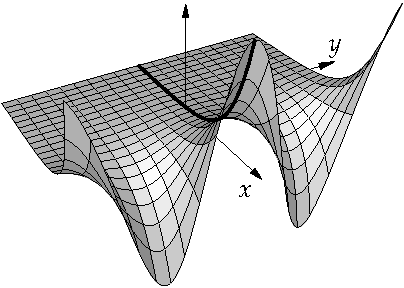
\includegraphics{figures/realexp}
\qquad
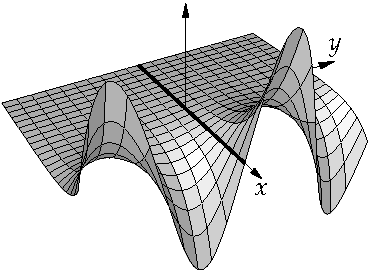
\includegraphics{figures/imagexp}
\caption{Graphs of the real part (left) and imaginary part (right)
of the complex exponential $e^z = e^{x+iy}$.
%The $x$-axis goes from $-4$ to $4$, the $y$-axis goes from $-6$ to $6$,
%and the vertical axis goes from $-e^{6} \approx -54.6$ to
%$e^{6} \approx 54.6$.
The plot of the real exponential ($y=0$)
is marked in a bold line.\label{fig:complexexpgraphs}}
\end{myfig}

This definition agrees with the standard definition for real numbers (when
$y=0$).  Furthermore,
\begin{equation*}
e^{\bar{z}} = 
e^{x-iy} =
e^x\cos y - i e^x \sin y  = \overline{e^{z}} ,
\end{equation*}
and
\begin{equation*}
\sabs{e^{z}} = 
\sabs{e^{x-iy}} =
e^x .
\end{equation*}
It is possible to not resort to the real exponentials, sines, and cosines
to define the complex exponential, and we will do so in due course.
But we want to have something to play around with now without waiting.

\begin{prop}
For any two complex numbers $z,w \in \C$,
\begin{equation*}
e^{z+w} = e^z e^w .
\end{equation*}
\end{prop}

\begin{exbox}
\begin{exercise}
Prove the proposition using the definition and trigonometric identities.
\end{exercise}
\end{exbox}

We remark that $e^z$ is the unique continuous
function on $\C$ that satisfies $e^{z+w} = e^z e^w$ and $e^0 = 1$.
But let us not worry about that.

For real $\theta$, the definition
of the exponential gives the so-called
\emph{\myindex{Euler's formula}}:
\begin{equation*}
e^{i\theta}
=
\cos \theta + i \sin \theta .
\end{equation*}
Using this formula we extend cosine and sine to the complex plane.
The formula says that for real $\theta$
\begin{equation*}
\cos \theta = \Re e^{i\theta} = \frac{e^{i\theta}+e^{-i\theta}}{2} ,
\qquad
\sin \theta = \Im e^{i\theta} = \frac{e^{i\theta}-e^{-i\theta}}{2i} .
\end{equation*}
We thus simply define cosine and sine for complex numbers by plugging
them into that formula, now that we know how to evaluate the exponential:
\begin{equation*}
\cos z \overset{\text{def}}{=} \frac{e^{iz}+e^{-iz}}{2} ,
\qquad
\sin z \overset{\text{def}}{=} \frac{e^{iz}-e^{-iz}}{2i} .
\end{equation*}


\subsection{Polar coordinates}

As complex numbers are just the plane, we can use polar coordinates
to represent complex numbers.
That is, $x = r \cos \theta$ and $y= r \sin \theta$.  We write this form as
\begin{equation*}
z = x+iy = r e^{i \theta} ,
\end{equation*}
where $r = \sabs{z} = \sqrt{x^2+y^2}$ is the \emph{\myindex{modulus}}, and 
$\theta$ is the angle that $x+iy$ makes with the real axis (the $x$-axis).
The $\theta$ is called the \emph{\myindex{argument}}.  See
\figureref{fig:polarcoords}.

\begin{myfig}
\subimport*{figures/}{polarcoords.pdf_t}
\caption{Polar coordinates.\label{fig:polarcoords}}
\end{myfig}

The reason for the notation is the
Euler's formula, so
\begin{equation*}
z = r e^{i\theta} = r\cos \theta + i r\sin \theta  = x+iy .
\end{equation*}

Polar form is particularly nice for multiplication of numbers and for powers.
Suppose $z = r e^{i\theta}$ and $w = s e^{i \psi}$, then
\begin{equation*}
zw =
r e^{i \theta} s e^{i \psi} = 
rs e^{i (\theta+ \psi)},
\qquad
\frac{1}{z} =
\frac{1}{r e^{i \theta}} =
\frac{1}{r} e^{-i \theta} ,
\qquad
z^n =
{\bigl(r e^{i \theta}\bigr)}^n =
r^n e^{i n\theta} .
\end{equation*}
In particular, again we see that multiplication by $i = e^{i \pi / 2}$ is
rotation counterclockwise by $90$ degrees.
The downside is that the polar form is particularly terrible for addition.
You win some, you lose some.

\begin{exbox}
\begin{exercise}
Let $z,w$ be two nonzero complex numbers and let
$\ell_z$ and $\ell_w$ be the lines through the origin and
$z$ and $w$ respectively.  Write $\theta$ for the angle between $\ell_z$ and
$\ell_w$.  Then prove that
$\Re z\bar{w} = \sabs{z} \sabs{w} \cos \theta$.
Note that $\Re z\bar{w}$ is the standard real dot product in $\R^2$, and so
this is the formula for the dot product from calculus.
\end{exercise}
\end{exbox}

\subsection{The argument}

We attempt to define the argument of $z = re^{i\theta}$ as
\glsadd{not:arg}%
\begin{equation*}
\arg z
\overset{\text{def?}}{=}
\theta ,
\end{equation*}
but we run up against the problem that if $\theta$ is an argument of $z$,
then so is $\theta+2\pi$ or $\theta + k 2\pi$ for any $k$.  In other words,
$\arg z$ is not a function in the classical sense, but a
\emph{\myindex{multivalued function}}%
\footnote{Non-complex analysts will sometimes claim that a multivalued
function is nonsense, but you can safely ignore them.}.  The correct
definition is
\glsadd{not:arg}%
\begin{equation*}
\arg z
\overset{\text{def}}{=}
\ldots,\theta - 4\pi,
\theta - 2\pi,
\theta ,
\theta + 2\pi,
\theta + 4\pi, \ldots
\end{equation*}
One more minor issue remains.  If $z=0$, then $z=0=0 e^{i\theta}$ for any
$\theta$ whatsoever.  Therefore, we only define the argument for nonzero
$z$.

It may at times be useful to nail down a particular number for the argument.
We define the \emph{\myindex{principal branch of $\arg$}} as
\glsadd{not:Arg}%
\begin{equation*}
\Arg z
\overset{\text{def}}{=}
\theta, \qquad \text{where } -\pi < \theta \leq \pi.
\end{equation*}
It may seem like a good solution to the multivaluedness of $\arg$, but
one's hopes are dashed by the cruel reality of $\Arg$ not being continuous
on the negative real axis.  See \figureref{fig:arggraph}.
The principal branch is somewhat less useful than one may think.
There is also the issue that not everyone agrees
on what ``principal branch'' means; some mathematicians sacrifice the
positive real axis and let $\theta$ be in the range $[0,2\pi)$.

\begin{myfig}
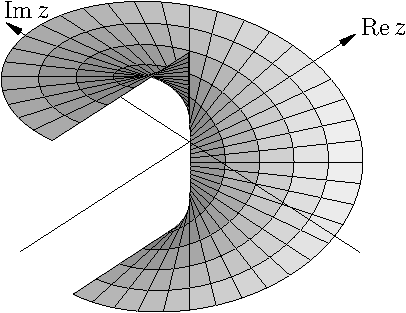
\includegraphics{figures/arggraph}
\caption{Graph of the principal branch of argument.\label{fig:arggraph}}
\end{myfig}

\begin{exbox}
\begin{exercise}
Show that $\Arg$ as defined above is not a continuous function on 
$\C \setminus \{ 0 \}$.
\end{exercise}
\end{exbox}

\subsection{Mapping properties of the exponential}

Let us consider what the exponential does to the complex plane.
The identity $e^{z+w} = e^z e^w$ implies that the exponential
is never zero (exercise).
From the known properties of polar coordinates
and the real exponential, it follows that the complex exponential is
onto $\C \setminus \{ 0 \}$.
The complex exponential is not one-to-one, it is 
infinitely-many-to-one.  For any integer $k$
\begin{equation*}
e^{z+ik2\pi} = 
e^{z} e^{ik2\pi} =
e^z .
\end{equation*}

\begin{exbox}
\begin{exercise}
Prove that the above are the only such identities by
showing that if $2k\pi < \Im z \leq 2(k+1)\pi$ and
$2k\pi < \Im w \leq 2(k+1)\pi$, then $e^z=e^w$ implies $z=w$.
\end{exercise}

\begin{exercise}
Use $e^{z+w} = e^z e^w$ and $e^0 = 1 \not= 0$ to show that $e^z \not=0$ for all
$z \in \C$.  In other words, if a function $f$ satisfies $f(z+w)=f(z)f(w)$
and $f(0) = 1$, then $f(z) \not= 0$ for all $z$.
\end{exercise}
\end{exbox}

Consider a vertical line given by $x=c$.  As
\begin{equation*}
e^{z} = 
e^{x+iy} =
e^x e^{iy} ,
\end{equation*}
and since $\sabs{e^{iy}} =1$, we find that the vertical line $x=c$ is taken to a
circle of radius $e^c$.  See \figureref{fig:expplotlines}.
Thus, the exponential takes the strip $a < x < b$ to the
annulus
\begin{equation*}
\bigl\{ z \in \C : e^a < \sabs{z} < e^b \bigr\} .
\end{equation*}

On the other hand, the horizontal line $y=c$
is taken to the ray from the origin to infinity where $\theta = c$ in polar
coordinates.  Again see \figureref{fig:expplotlines}.
Hence, the exponential takes the strip $a < y < b$ to the
sector
\begin{equation*}
\bigl\{ z \in \C : ``a < \arg z < b'' \bigr\} .
\end{equation*}
The reason for the quotation marks is that the inequality makes no
sense without interpreting it properly.  It means that one of the values
of $\arg z$ is between $a$ and $b$.

In particular, the exponential $e^z$ takes the set given by
$2k\pi < \Im z \leq 2(k+1)\pi$ in a one-to-one (see the exercise above)
way onto $\C \setminus \{ 0 \}$.

\begin{myfig}
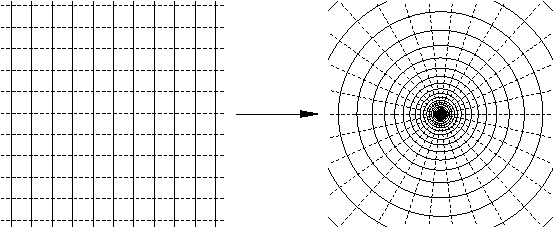
\includegraphics{figures/expplotlines}
\caption{Horizontal and vertical lines mapped by the exponential.  Note that
each horizontal line only goes to a ray from the
origin.\label{fig:expplotlines}}
\end{myfig}

%%%%%%%%%%%%%%%%%%%%%%%%%%%%%%%%%%%%%%%%%%%%%%%%%%%%%%%%%%%%%%%%%%%%%%%%%%%%%%

\section{The Riemann sphere}

It is sometimes useful to extend the real numbers by adding $\pm \infty$.
A similar concept exists for the complex plane, although
we only add one infinity.  We write
\glsadd{not:Cinfty}%
\glsadd{not:infty}%
\begin{equation*}
\C_{\infty} = \C \cup \{ \infty \} ,
\end{equation*}
and we call $\C_{\infty}$ the \emph{\myindex{Riemann sphere}}.
We want to define the topology of $\C_\infty$ to be the same as that of $\C$
when we are away from infinity.
We define the function $g \colon \C_\infty \to \C_\infty$ by
\begin{equation*}
g(z) =
\begin{cases}
\frac{1}{z} & \text{if } z \not= 0 \text{ and } z \not= \infty, \\
\infty & \text{if } z = 0, \\
0 & \text{if } z = \infty.
\end{cases}
\end{equation*}
The function $g$ is bijective (one-to-one and onto).
Any neighborhood of the origin in $\C$ is taken to a set that
includes infinity and we call those the neighborhoods of
$\infty$.  When talking about a neighborhood of
infinity in $\C_{\infty}$, then we really want to think of this map,
and think of the corresponding neighborhood of the origin.

More concretely, we can give $\C_{\infty}$ a metric space structure.
Let $S^2$ be the unit sphere in $\R^3$,
that is, the set described by $x^2 + y^2 + z^2 = 1$ if $(x,y,z)$ are the
coordinates.\footnote{This is possibly the only instance in this book where
$z$ is a real number.}  The plane $\R^2$ with coordinates $(x,y)$ can be
identified with $\C$ with coordinate $\xi$ by taking $x+iy = \xi$.
Given any point $p \in S^2$ that is not the north pole $(0,0,1) \in S^2$,
there is a unique line in $\R^3$ through the point $(0,0,1)$ and $p$.
It is not difficult to prove that this line is never parallel to the
$xy$-plane, that is, to $\C$, and hence it must intersect $\C$ in a unique
point $\xi \in \C$ (a plane and a line intersect at a unique point unless
the two are parallel).  We define:
\begin{equation*}
\Phi(p) = \xi.
\end{equation*}
We let $\Phi\bigl((0,0,1)\bigr) = \infty$ so that we have a map
$\Phi \colon S^2 \to \C_\infty$.  This map is called the 
\emph{\myindex{stereographic projection}}.  See
\figureref{fig:riemannsphere}.
The map is bijective (exercise below),
and so we define a metric in $\C_\infty$ by
using a metric on $S^2$, which we can just take to be the subspace
metric coming from the euclidean metric on $\R^3$ (another possibility
could be the great circle distance, \exampleref{ms:greatcircle}).

\begin{myfig}
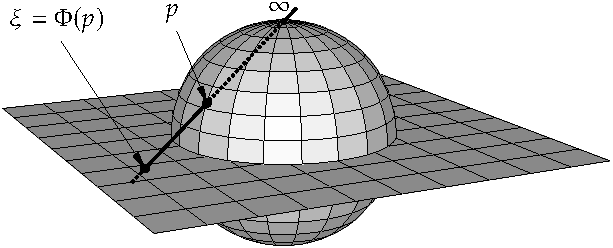
\includegraphics{figures/riemannsphere}
\caption{Stereographic projection of the Riemann sphere to the complex plane.\label{fig:riemannsphere}}
\end{myfig}

\begin{exbox}
\begin{exercise}
Show that $\Phi$ is bijective.
\end{exercise}

\begin{exercise}
Suppose $(\phi,\theta)$
are spherical coordinates on $S^2$, where $0 \leq \phi \leq \pi$ is the zenith (angle made
with the $z$-axis) and $-\pi < \theta \leq \pi$ the azimuth, and we write
points in $\C$ using polar coordinates $re^{\theta}$.  Then prove that $\Phi$ of
$(\phi,\theta)$ is $(\cot \nicefrac{\phi}{2})e^{i\theta}$.
\end{exercise}

\begin{exercise}
Show that the topology induced on $\C$ by the topology of $S^2$ using $\Phi$
as above is equivalent to the standard one.  That is, show that a set $U
\subset \C$
is open in the euclidean metric on $\C$ if and only if it is open using the
metric coming from $S^2$.
\end{exercise}
\end{exbox}

The point of the Riemann sphere is to give the value $\infty$ to certain
limits and to allow limits as $z$ tends to $\infty$.  For a
function $f \colon U \subset \C_\infty \to \C_\infty$, we define
\begin{equation*}
\lim_{z \to z_0} f(z) = L
\end{equation*}
as the metric space limit using the metric on the Riemann sphere, 
including
the cases when $z_0 = \infty$, $L = \infty$, or both.
Conveniently the Riemann sphere is compact.
Indeed, topologically, it is the same as the
``one-point compactification'' of $\C$.

\begin{exbox}
\begin{exercise}
Suppose that $L \in \C$ and $z_0 \in \C$.
Show that $\lim_{z\to z_0} f(z) = L$ in the sense of the Riemann sphere
if and only if $\lim_{z \to z_0} f(z) = L$ in the usual sense (the euclidean
metric on $\C$).
\end{exercise}

\begin{exercise}
Suppose that $L \in \C$.
Show that $\lim_{z\to \infty} f(z) = L$ in the sense of the Riemann sphere
if and only if, for every $\epsilon > 0$ there exists an $M$ such that
$\sabs{f(z)-L} < \epsilon$ whenever $\sabs{z} > M$.
\end{exercise}

\begin{exercise}
Suppose that $z_0 \in \C$.
Show that $\lim_{z\to \infty} f(z) = \infty$ in the sense of the Riemann sphere
if and only if, for every $M > 0$ there exists a $\delta > 0$ such that
$\sabs{f(z)} > M$ whenever $\sabs{z-z_0} < \delta$.
\end{exercise}

\begin{exercise}
Show that $\lim\limits_{z\to\infty} f(z) = L$ for some $L \in \C_\infty$ if and only if
$\lim\limits_{z \to 0} f(\nicefrac{1}{z}) = L$.
\end{exercise}

\begin{exercise}
Show that $\lim\limits_{z\to z_0} f(z) = \infty$ for some $z_0 \in \C_\infty$ if and only if
$\lim\limits_{z \to z_0} \frac{1}{f(z)} = 0$.
\end{exercise}
\end{exbox}

It then makes sense to talk about the value of $\frac{1}{z}$ at the origin
as $\infty$, and the value of $z$ at $\infty$ as $\infty$.
In fact, any nonconstant polynomial is $\infty$ at $\infty$.

\begin{exbox}
\begin{exercise} \label{exercise:polygoesinf}
Suppose $P(z) = a_d z^d + a_{d-1} z^{d-1} + \cdots + a_1 z + a_0$ be
a polynomial where $a_0,\ldots,a_d \in \C$.  Prove that if $d \geq 1$
and $a_d \not=0$ ($P$ is nonconstant),
then $\lim_{z \to \infty} P(z) = \infty$.
Hint: If $a_d = 1$, then using
$\abs{\frac{a_{d-1} z^{d-1} + \cdots + a_1 z + a_0}{z^d}}$, one finds
$\abs{P(z)} \geq \frac{1}{2} \sabs{z}^d$ for large $z$.
\end{exercise}
\end{exbox}

In calculus and in basic real analysis, you likely encountered
infinite limits in the sense of the extended reals.
Despite that the two types of infinite limits, either in the sense of the
extended reals or in the sense of the Riemann sphere,
look similar, and despite using essentially the same notation,
they are different.
For example,
\begin{equation*}
\lim_{x \to 0} \frac{1}{x} \quad \text{does not exist,} \qquad \text{but} \qquad
\lim_{z \to 0} \frac{1}{z} = \infty .
\end{equation*}
Here on the left hand side we tacitly use the extended real sense
($x$ is real, no?) and on the
right hand side we tacitly use the Riemann sphere sense ($z$ seems complex).
This could, obviously, cause confusion.
In this book, infinite limits are going to be in the Riemann sphere sense
unless either otherwise noted or obvious.

\medskip

The arithmetic that one can 
reasonably define with the Riemann sphere $\infty$ is quite different from
the $\infty$ of the extended reals.
No additions or subtractions make sense here.
Even something like
$\infty+\infty$ does not make sense, even though this is common for the
extended reals:  For example, if $f(z) = z$ and $g(z) = -z$,
then $\lim_{z \to \infty} f(z) = \infty$,
$\lim_{z \to \infty} g(z) = \infty$, but $\lim_{z \to \infty}
\bigl(f(z)+g(z)\bigr) = 0$.

On the other hand it is reasonable to define $\frac{c}{0} = \infty$ for
any $c \not= 0$, $\frac{c}{\infty} = 0$ for any $c \not= \infty$,
and $c \cdot \infty = \infty$ for any $c \not= 0$.
Just make sure to definitely avoid doing any additions and subtractions of
infinities!

%%%%%%%%%%%%%%%%%%%%%%%%%%%%%%%%%%%%%%%%%%%%%%%%%%%%%%%%%%%%%%%%%%%%%%%%%%%%%%

\section{Linear fractional transformations}

A convenient set of transformations of the complex plane or the Riemann
sphere are the \emph{\myindex{linear fractional transformations}} (LFT)\index{LFT}
(sometimes called the \emph{\myindex{M\"obius transformations}}).
A function
\begin{equation*}
f(z) = \frac{a z + b}{c z + d}
\end{equation*}
is a linear fractional transformation if $ad \not= bc$.  The requirement on
$a$, $b$, $c$, $d$ guarantees that the ratio does not simplify and that the
function is nonconstant.

If $c\not=0$,
the expression is normally defined only on
$\C \setminus \bigl\{ \frac{-d}{c} \bigr\}$,
however, as in the last section, we write
\begin{equation*}
f\left(\frac{-d}{c}\right) = \infty, \qquad \text{and} \qquad
f(\infty) = \frac{a}{c} .
\end{equation*}
If $c=0$, then set $f(\infty) = \infty$.  In either case, $f$ is a map of
the Riemann sphere to itself.

\begin{exbox}
\begin{exercise}
Prove that an LFT is a bijective mapping of the Riemann sphere to itself.
\end{exercise}

\begin{exercise}
Prove that an LFT extended to the Riemann sphere as above is continuous.
\end{exercise}
\end{exbox}

Any LFT is a composition of \emph{translations}\index{translation}
\begin{equation*}
T_a(z) = z + a ,
\end{equation*}
\emph{complex dilations}\index{complex dilation}
\begin{equation*}
D_a(z) = az ,
\end{equation*}
and \emph{inversions}\index{inversion}
\begin{equation*}
I(z) = \frac{1}{z}.
\end{equation*}
Suppose $f(z) = \frac{az+b}{cz+d}$ is an LFT.
Without loss of generality, we assume that either $c=1$ or $c=0$.
Suppose $c=1$ first,
\begin{equation*}
f(z)
=
\frac{a z + b}{z + d}
=
\frac{b-ad}{z+d}+a
=
T_a\biggr(D_{b-ad}\Bigr(I\bigl(T_d(z)\bigr)\Bigr)\biggr) .
\end{equation*}
If $c=0$, then we can also assume that $d=1$ and
so $f(z) = az + b$.
Then
\begin{equation*}
f(z) = az+b = T_b\bigl(D_a(z)\bigr) .
\end{equation*}

This sort of decomposition is quite useful in proving statements about
LFTs that are preserved under composition,
one only needs to prove it for $T_a$, $D_a$, and $I$.  This technique
will come in handy in just the next exercise.

Let us include straight lines in the set of circles.  After all, a straight
line is just a circle through infinity: Think about the circle of radius $r$
centered at $ir$ as $r \to \infty$.  Then an LFT takes circles to circles.
We leave this fact as an exercise.

\begin{exbox}
\begin{exercise}
Prove that if we include straight lines in the set of ``circles'', then
an LFT takes circles to circles.
\end{exercise}

\begin{exercise} \label{exercise:anycircletorealline}
Prove that given any circle or a straight line, there exists an LFT
that takes that circle or line to the real line.
\end{exercise}
\end{exbox}

One way to view an LFT is as a $2 \times 2$ complex matrix.  For this purpose
we need to view the Riemann sphere as the so-called one-dimensional
\emph{\myindex{projective space}}.
Define the equivalence relation $\sim$ on $\C^2 \setminus \{ 0 \}$ by
$u \sim v$ if and only if $u = \lambda v$ for some $\lambda \in \C$.
The \emph{\myindex{one-dimensional complex projective}}
space is then defined by
\glsadd{not:CP1}%
\begin{equation*}
\C \bP^1
\overset{\text{def}}{=}
\faktor{\C^2 \setminus \{ 0\}}{\sim} \ .
\end{equation*}
In other words, $\C \bP^1$ is the set of ``complex lines through the
origin'' in $\C^2$, or yet in other words,
it is the set of one-dimensional vector
subspaces of $\C^2$.

We identify $\C\bP^1$ with $\C_\infty$ in the following
way.  Denote by $[z:w] \in \C \bP^1$
the equivalence class of vectors in $\C^2$ under
$\sim$ that contains $(z,w) \in \C^2$.
Then define the map $\Phi \colon \C_\infty \to \C \bP^1$ as
\begin{equation*}
\Phi(z) =
\begin{cases}
[z:1] & \text{if } z \in \C , \\
[1:0] & \text{if } z=\infty .
\end{cases}
\end{equation*}

\begin{exbox}
\begin{exercise}
Prove that $\Phi$ above is bijective.
\end{exercise}
\end{exbox}

Let us check that an LFT
\begin{equation*}
f(z) = \frac{a z + b}{c z + d}
\end{equation*}
corresponds to an invertible linear map given by the matrix
\begin{equation*}
M =
\begin{bmatrix}
a & b \\
c & d
\end{bmatrix} .
\end{equation*}
An invertible $M$ takes one-dimensional subspaces to one-dimensional
subspaces, so it sounds plausible.

First, $\Phi \circ f$ for $z \in \C \setminus \bigl\{ \frac{-d}{c} \bigr\}$
is equal to
\begin{equation*}
\Phi \circ f(z) =
\left[\frac{a z + b}{c z + d}: 1 \right]
=
\left[a z + b: c z + d \right] ,
\end{equation*}
where the second inequality follows by definition of $\sim$.
When $z = \frac{-d}{c}$, then $cz+d = 0$, or $f(0) = \infty$
and $\Phi(\infty) = [1:0] = [az+b : cz+d]$ as well.

Let us consider $\Phi \circ f \circ \Phi^{-1}$.
If $w \not= 0$, then $[z:w] = \left[ \frac{z}{w}:1 \right]$.  So
\begin{equation*}
\Phi \circ f \circ \Phi^{-1} \bigl([z:w]\bigr) =
\Phi \circ f \left(\frac{z}{w}\right) =
\left[a \frac{z}{w} + b : c \frac{z}{w} + d \right] =
\left[a z + b w: c z + d w \right] .
\end{equation*}
And one checks that the same equality holds if $w=0$.
As
$M \left[ \begin{smallmatrix} z \\ w \end{smallmatrix} \right]
= \left[ \begin{smallmatrix} 
a z + b w \\ c z + d w
\end{smallmatrix} \right]$,
the function $f$ corresponds to the linear map $v \mapsto Mv$ on $\C^2$.
The requirement $ad \not= bc$ implies $\det M \not= 0$,
or in other words, $M$ is invertible.
So every LFT is represented by an invertible $2 \times 2$ matrix $M$
(not uniquely), and
conversely every invertible $2 \times 2$ matrix $M$ corresponds to an LFT.

An invertible $2 \times 2$ matrix $M$ gives a map from
$\C^2 \setminus \{ 0 \}$ to $\C^2 \setminus \{ 0 \}$.
Let $\pi \colon \C^2 \setminus \{ 0 \} \to \C \bP^1$ be the map\footnote{The
``quotient map'' or the ``natural projection.''}
$\pi \bigl( (z,w) \bigr) =
[z:w]$.  The following commutative diagram may
illustrate the entire situation better:
\begin{equation*}
\begin{tikzcd}
\C^2 \setminus \{ 0 \} \arrow[r,"M"] \arrow[d,"\pi"] &
\C^2 \setminus \{ 0 \} \arrow[d,"\pi"] \\
\C \bP^1 \arrow[r,"\Phi \circ f \circ \Phi^{-1}"] \arrow[d,shift left,"\Phi^{-1}"] &
\C \bP^1 \arrow[d,shift left,"\Phi^{-1}"]
\\
\C_\infty \arrow[r,"f"]\arrow[u,shift left,"\Phi"] &
\C_\infty \arrow[u,shift left,"\Phi"]
\end{tikzcd}
\end{equation*}

\medskip

A handy LFT is the
\emph{\myindex{Cayley map}}:
\begin{equation*}
C(z)
=
\frac{z - i}{z + i} .
\end{equation*}
The map is clearly an LFT, and it
takes the upper half-plane $\bH = \{ z \in \C : \Im z > 0 \}$ to the
unit disc $\D$.  Let us see why.  The map takes $z \in \C$ to the unit disc if
\begin{equation*}
1 > \abs{\frac{z - i}{z + i} }
=
\frac{\sabs{z - i}}{\sabs{z + i}} .
\end{equation*}
In other words, $\sabs{z+i} > \sabs{z - i}$: The distance of $z$
to $-i$ is larger than the distance of $z$ to $i$.  It is straightforward
plane geometry to see this means that $z \in \bH$.  See
\figureref{fig:cayleydisc}.

\begin{myfig}
\subimport*{figures/}{cayleydisc.pdf_t}
\caption{Why does the Cayley map take $\bH$ to $\D$.\label{fig:cayleydisc}}
\end{myfig}

Any LFT is bijective if thought of as a map from $\C_\infty$
to itself, so $C^{-1}$ exists, and it is also a useful map.  We leave
it as an exercise to figure out the inverse.

\begin{exbox}
\begin{exercise}
Figure out what $C^{-1}$ is.  Hint: Think of $\C_\infty$ as $\C \bP^1$
and $C$ as a matrix.  It is really easy to invert $2 \times 2$ matrices.
\end{exercise}

\begin{exercise}
For any LFT $f(z) = \frac{az+b}{cz+d}$ find $f^{-1}$.
Hint: Same hint as above.
\end{exercise}
\end{exbox}

In the exercises you have essentially just shown (or at least finished
showing) that LFTs form a group under composition,
called the \emph{\myindex{M\"obius group}}.
This group is generated by the elements
$T_a$, $D_a$, and $I$ for $a\in \C$.

%%%%%%%%%%%%%%%%%%%%%%%%%%%%%%%%%%%%%%%%%%%%%%%%%%%%%%%%%%%%%%%%%%%%%%%%%%%%%%

\section{Cross ratio *}

There is a certain quantity that is preserved by LFTs, the
\emph{\myindex{cross ratio}}:
\glsadd{not:crossratio}%
\begin{equation*}
(z_1,z_2;z_3,z_4)
=
\frac{(z_3-z_1)(z_4-z_2)}{(z_3-z_2)(z_4-z_1)}
=
\frac{z_3-z_1}{z_3-z_2} : 
\frac{z_4-z_1}{z_4-z_2} ,
\end{equation*}
where $z_1,z_2,z_3,z_4$ are complex numbers.  The cross ratio
was already described by the ancient Greeks and plays a key role in
projective geometry.
The definition is extended to when one of the numbers is $\infty$ by simply
erasing the affected terms from the ratios.  Pretend that say $z_3-\infty$
is really equal to $z_4-\infty$ and thus they cancel.
\begin{align*}
(\infty,z_2;z_3,z_4)
& =
\frac{z_4-z_2}{z_3-z_2}
,
&
(z_1,\infty;z_3,z_4)
& =
\frac{z_3-z_1}{z_4-z_1}
,
\\
(z_1,z_2;\infty,z_4)
& =
\frac{z_4-z_2}{z_4-z_1}
,
& 
(z_1,z_2;z_3,\infty)
& =
\frac{z_3-z_1}{z_3-z_2} .
\end{align*}

By ``preserved by LFTs'' we mean that if $f(z)$ is an LFT then
\begin{equation*}
(z_1,z_2;z_3,z_4) =
\bigl(f(z_1),f(z_2);f(z_3),f(z_4)\bigr) .
\end{equation*}

\begin{exbox}
\begin{exercise}
Prove the invariance of cross ratios under LFTs.
\end{exercise}

\begin{exercise}
Prove that four distinct points are on a line or a circle if and only if the cross
ratio is real.
Hint: The exercise above and \exerciseref{exercise:anycircletorealline}.
\end{exercise}
\end{exbox}

Cross ratios give a convenient way to describe LFTs.  For example, 
for three distinct numbers $z_2,z_3,z_4$, the
function
\begin{equation*}
f(z) =
(z,z_2;z_3,z_4)
\end{equation*}
is an LFT such that $f(z_2) = 1$, $f(z_3)=0$ and $f(z_4) = \infty$.
In other words,
$(z,z_2;z_3,z_4) = 
\bigl(f(z),1;0,\infty\bigr)$.

\begin{exbox}
\begin{exercise}
Given two sets of distinct points $z_1,z_2,z_3 \in \C_\infty$
and $w_1,w_2,w_3 \in \C_\infty$, explicitly find an LFT $f$,
such that
$f(z_1) = w_1$,
$f(z_2) = w_2$, and
$f(z_3) = w_3$.
\end{exercise}

\begin{exercise}
Given distinct points $z_1,z_2,z_3 \in \C$ and
using the cross ratio definition of an LFT, explicitly find
the equation of a circle (or the straight line) through the three points.
Hint: Inverse image of the real line is a circle or a straight line.
\end{exercise}
\end{exbox}


%%%%%%%%%%%%%%%%%%%%%%%%%%%%%%%%%%%%%%%%%%%%%%%%%%%%%%%%%%%%%%%%%%%%%%%%%%%%%%
%%%%%%%%%%%%%%%%%%%%%%%%%%%%%%%%%%%%%%%%%%%%%%%%%%%%%%%%%%%%%%%%%%%%%%%%%%%%%%
%%%%%%%%%%%%%%%%%%%%%%%%%%%%%%%%%%%%%%%%%%%%%%%%%%%%%%%%%%%%%%%%%%%%%%%%%%%%%%

\chapter{Holomorphic and Analytic Functions} \label{ch:holanal}

\begin{myquote}
If this is coffee, please bring me some tea; but if this is tea, please bring me some coffee.

---Abraham Lincoln
\end{myquote}

%%%%%%%%%%%%%%%%%%%%%%%%%%%%%%%%%%%%%%%%%%%%%%%%%%%%%%%%%%%%%%%%%%%%%%%%%%%%%%

\section{Holomorphic functions and Cauchy--Riemann}
\label{sec:holfuncs}

\subsection{Holomorphic functions}

The functions we wish to study are those that in some sense
generalize polynomials in $z \in \C$;  we wish to study functions
that,
at least locally, behave like $P(z) = a_n z^n + a_{n-1} z^{n-1} + \cdots +
a_1 z + a_0$.  Polynomials are easy to understand and easy to work
with.  Unfortunately there aren't that many of them.  For example, there is
no polynomial that solves the most basic of differential equations: $f' =
f$.  So we must enlarge our horizons a bit.

Consider a polynomial $P(z)$ and expand it near some $z_0 \in \C$:
\begin{equation*}
P(z) = c_0 + c_1 (z-z_0) + c_2 {(z-z_0)}^2 + \cdots + c_n {(z-z_0)}^n .
\end{equation*}
So $P(z_0+h) = c_0 + c_1 h + c_2 h^2 + \cdots + c_n h^n$.
Then
\begin{equation*}
\lim_{h \to 0} \frac{P(z_0+h) - P(z_0)}{h} =
\lim_{h \to 0} \frac{P(z_0+h) - c_0}{h} = c_1 .
\end{equation*}
So $P(z_0+h)$ is approximated (locally) by $c_0 + c_1 h$
up to an error that vanishes faster than $h$.
We should emphasize that the limits are as a complex $h$ goes to $0$.

Therefore, we wish to study functions that are
locally approximated by $c_0 + c_1 h$ in the same way.  More formally
we want functions such that
\begin{equation*}
f(z_0+h) = f(z_0) + \xi h + o(\sabs{h})
\end{equation*}
for some $\xi \in \C$, where $o(\sabs{h})$ means any function of $h$
that goes to zero faster than $\sabs{h}$.

\begin{defn}
Suppose $U \subset \C$ is open.
Given $f \colon U \to \C$ and $z_0 \in U$, we say 
$f$ is \emph{\myindex{complex differentiable}} at $z_0$ if
the limit
\glsadd{not:cplxder}%
\begin{equation} \label{eq:complexdiff}
f'(z_0) \overset{\text{def}}{=}
\lim_{h \to 0} \frac{f(z_0+h) - f(z_0)}{h} \qquad ( = \xi )
\end{equation}
exists.
We call $f'(z_0)$ the \emph{\myindex{complex derivative}} of $f$
at $z_0$.

A function $f \colon U \to \C$ is
\emph{\myindex{holomorphic}}
if it is complex differentiable at every point.  That is, if
\eqref{eq:complexdiff} exists for all $z_0 \in U$.
%We will write
%the set of holomorphic functions defined on $U$ as $\sO(U)$.
%FIXME: do we every really use $\sO(U)$
\end{defn}

Above, we proved the following proposition that justifies our motivation
for the complex derivative:

\begin{prop}
If $P(z)$ is a polynomial, then $P \colon \C \to \C$ is holomorphic.
\end{prop}

The most basic result about holomorphic functions is that they are
continuous.
This can be proved (exercise) either directly from the definition,
or using that a holomorphic function is
(real) differentiable as we will see shortly.

\begin{prop}
If $U \subset \C$ is open and $f \colon U \to \C$ is holomorphic, then $f$
is continuous.
\end{prop}

\begin{exbox}
\begin{exercise}
Directly from the definition of the complex derivative, show that a
holomorphic function is continuous (prove the proposition above).
\end{exercise}

\begin{exercise}
Show that $f(z) = \bar{z}$ is not complex differentiable at any point.
\end{exercise}

\begin{exercise}
Show that $f(z) = z \bar{z} = \sabs{z}^2$ is complex differentiable
at the origin, but nowhere else.
\end{exercise}
\end{exbox}

\subsection{Cauchy--Riemann equations}

Suppose $U \subset \C$ is open, and
let $f \colon U \to \C$ be a
differentiable (in the real sense
and as a function of two real variables,
see \sectionref{sec:derinsv} in the appendix) function.
If we think of $\C$ as $\R^2$,
then the real derivative of $f$ is a $2 \times 2$ real matrix $D f$.
That is, $f$ is (real) differentiable at $z_0$ if there exists
a $2 \times 2$ real matrix $Df|_{z_0}$ such that
\begin{equation*}
\lim_{h \to 0} \frac{\sabs{f(z_0+h) - f(z_0) - (Df|_{z_0}) h}}{\sabs{h}} = 0 .
\end{equation*}
We think of $h$ as a column vector in $\R^2$ 
to be able to apply it to the
$2 \times 2$ real matrix $Df|_{z_0}$.
A key point here is that the limit is being taken
as $h$ moves in $\C$ (or $\R^2$ if you wish).
So $f(z_0+h) - f(z_0) - (Df|_{z_0}) h$ is $o(\sabs{h})$ as needed.
The trick is to see when $(Df|_{z_0}) h$ corresponds to $\xi h$
for some $\xi \in \C$.

Write $f = u+iv$, that is, as a
mapping into $\R^2$ it is $f = (u,v)$.  Then
\begin{equation*}
Df|_{z_0} =
\begin{bmatrix}
\frac{\partial u}{\partial x}\big|_{z_0} & \frac{\partial u}{\partial
y}\big|_{z_0} \\[5pt]
\frac{\partial v}{\partial x}\big|_{z_0} & \frac{\partial v}{\partial y}\big|_{z_0}
\end{bmatrix} .
\end{equation*}
As we have seen in the last chapter, only a matrix of the form
$\left[ \begin{smallmatrix}
a & -b \\ b & a
\end{smallmatrix} \right]$ corresponds to multiplication a complex number $a+ib$.
So the derivative $Df|_{z_0}$ corresponds to multiplication by a
complex number only if it is of the form
$\left[ \begin{smallmatrix}
a & -b \\ b & a
\end{smallmatrix} \right]$, or in other words,
\begin{equation*}
\frac{\partial u}{\partial x}\Big|_{z_0} =
\frac{\partial v}{\partial y}\Big|_{z_0}
, \qquad
\frac{\partial v}{\partial x}\Big|_{z_0} =
-\frac{\partial u}{\partial y}\Big|_{z_0} .
\end{equation*}
In this case $Df|_{z_0}$ corresponds to multiplication by the number
$\xi = \frac{\partial u}{\partial x}\big|_{z_0} + i \frac{\partial v}{\partial
x}\big|_{z_0}$, which is equal to
$\frac{\partial v}{\partial y}\big|_{z_0} - i \frac{\partial u}{\partial
y}\big|_{z_0}$.
So we get that
\begin{equation*}
0 = \lim_{h \to 0} \frac{\sabs{f(z_0+h) - f(z_0) - \xi h}}{\sabs{h}} =
\lim_{h \to 0} \abs{\frac{f(z_0+h) - f(z_0)}{h} - \xi} ,
\end{equation*}
or in other words
\begin{equation*}
\lim_{h \to 0} \frac{f(z_0+h) - f(z_0)}{h} = \xi .
\end{equation*}
So $f$ is complex differentiable at $z_0$ and $f'(z_0) = \xi$.

We proved that if $f$ is differentiable at $z_0$ (in the real sense), then 
the complex derivative exists at $z_0$ if and only if 
$\frac{\partial u}{\partial x}\big|_{z_0} = \frac{\partial v}{\partial
y}\big|_{z_0}$ and $\frac{\partial v}{\partial x}\big|_{z_0} = -\frac{\partial
u}{\partial y}\big|_{z_0}$.
%We usually want to do this at all points, not just one.
By working backwards, it is immediate
that if $f$ is complex differentiable at $z_0$, then it is real
differentiable at $z_0$,
as the complex derivative $f'(z_0)$ gives the $Df|_{z_0}$.  Let us formalize
what we just proved.

\begin{prop}
Let $U \subset \C$ be open and $f = u+iv \colon U \to \C$ be a function.
Then
$f$ is complex differentiable at $z_0 \in U$
if and only if
$f$ (real) differentiable at $z_0 \in U$
with
$\frac{\partial u}{\partial x}\big|_{z_0} =
\frac{\partial v}{\partial y}\big|_{z_0}$
and
$\frac{\partial v}{\partial x}\big|_{z_0} =
-\frac{\partial u}{\partial y}\big|_{z_0}$ .
\end{prop}

If the partial derivatives exist and are continuous, then $f$ is
(real) differentiable (see \sectionref{sec:derinsv} again).
So we have the following, perhaps easier to apply, result.

\begin{cor}
Let $U \subset \C$ be open and let $f = u+iv \colon U \to \C$ be a function
such that $\frac{\partial u}{\partial x}$, $\frac{\partial u}{\partial y}$, $\frac{\partial
v}{\partial x}$, and $\frac{\partial v}{\partial y}$ exist and are continuous (that is,
$f$ is continuously differentiable).
Then
\begin{equation} \label{eq:CReqreal}
\frac{\partial u}{\partial x} = \frac{\partial v}{\partial y} , \qquad
\frac{\partial v}{\partial x} = -\frac{\partial u}{\partial y}
\end{equation}
if and only if $f$ is complex differentiable at all $z \in U$, or in
other words, if
\begin{equation*}
f'(z) =
\lim_{h \to 0} \frac{f(z+h) - f(z)}{h}
\qquad
\text{exists for all $z \in U$.}
\end{equation*}
\end{cor}

The equations \eqref{eq:CReqreal} are called the
\emph{\myindex{Cauchy--Riemann equations}}\footnote{Interestingly,
the equations first appeared in the work of d'Alembert, and
it was Euler who first connected them to analytic functions.
So perhaps they had better be called the French-guy--German-guy equations,
except that Euler was really Swiss, he only lived in Germany for a long time.}.
This book is dedicated to their
solutions.

So continuously differentiable functions that satisfy
Cauchy--Riemann equations are holomorphic.
On the other hand
a function that is complex differentiable everywhere (a holomorphic
function) is differentiable in the real sense,
and thus the partial derivatives exist and satisfy the Cauchy--Riemann
equations.  We will show later that holomorphic functions are
continuously differentiable and not just differentiable, and in fact they
are infinitely differentiable.

\begin{exbox}
\begin{exercise} \label{exercise:exponentialholomorphic}
Show that the complex exponential function, and hence also sine and cosine,
is holomorphic, and show that $\exp' = \exp$.
\end{exercise}

\begin{exercise}
Let $U \subset \C$ be a domain (open and connected),
and $f \colon U \to \R$ be a real-valued function that is holomorphic.
Prove that $f$ is constant.
\end{exercise}

\begin{exercise}
Let $U \subset \C$ be open and $f \colon U \to \C$ holomorphic.
Write $f = u+iv$.  Show that $u$ and $v$ are \emph{\myindex{harmonic}},
that is,
$\frac{\partial^2 u}{\partial x^2} +  \frac{\partial^2 u}{\partial y^2} = 0$
and
$\frac{\partial^2 v}{\partial x^2} +  \frac{\partial^2 v}{\partial y^2} = 0$.
Feel free to assume that both $u$ and $v$ are twice continuous
differentiable.
\end{exercise}

\begin{exercise}
Let $U \subset \C$ be open and $f \colon U \to \C$ holomorphic.
Write $f = u+iv$.  Show that whenever the second derivative test applies 
to $u$ or $v$, you get a saddle, that is, prove that
$\frac{\partial^2 u}{\partial x^2} \frac{\partial^2 u}{\partial y^2}
-{\left(\frac{\partial^2 u}{\partial x \partial y}\right)}^2 \leq 0$
and
$\frac{\partial^2 v}{\partial x^2} \frac{\partial^2 v}{\partial y^2}
-{\left(\frac{\partial^2 v}{\partial x \partial y}\right)}^2 \leq 0$.
Feel free to assume that both $u$ and $v$ are twice continuous
differentiable.
\end{exercise}

\begin{exercise}
\begin{exparts}
\item
Show that in polar coordinates $z=re^{i\theta}$,
the Cauchy--Riemann equations (outside the origin) on $f=u+iv$ are
\begin{equation*}
\frac{\partial u}{\partial r} = \frac{1}{r} \frac{\partial v}{\partial \theta},
\qquad
\frac{\partial v}{\partial r} = \frac{-1}{r} \frac{\partial u}{\partial \theta}.
\end{equation*}
\item
Use the computation to (locally) find the form of all solutions to 
the Cauchy--Riemann equations where $\Re f = u$ does not depend on the
argument $\theta$.  By locally we mean only in some neighborhood $U$ of a
point $p \not= 0$.
\end{exparts}
\end{exercise}
\end{exbox}


%%%%%%%%%%%%%%%%%%%%%%%%%%%%%%%%%%%%%%%%%%%%%%%%%%%%%%%%%%%%%%%%%%%%%%%%%%%%%%

\section{Basic properties of holomorphic functions}

\subsection{Elementary calculus}

First, let us solve a differential equation.  A common technique in analysis
to show an equality is to differentiate and then show that the derivative is
zero.

\begin{prop} \label{prop:zeroder}
Let $U \subset \C$ be a domain (open and connected),
and $f \colon U \to \C$ be holomorphic, and $f'(z) = 0$ for all $z \in U$.
Then $f$ is a constant.
\end{prop}

\begin{proof}
Follows from the standard real result,
see \thmref{thm:svzerodersol} in the appendix.
\end{proof}

\begin{prop}[Chain rule] \index{chain rule!complex derivative}
Let $U \subset \C$ and $V \subset \C$ be open, $f \colon U \to V$
complex differentiable at $z \in U$, and $g \colon V \to \C$ complex differentiable
at $f(z)$.  Then the composition $g \circ f$
is complex differentiable at $z$ and $(g \circ f)'(z) = g'\bigl(f(z)\bigr) f'(z)$.
\end{prop}

\begin{proof}
We offer two proofs.  The first works only for holomorphic
functions, and the second is generalizable to nonholomorphic functions
with the Wirtinger operators in the next section (an exercise).

Let $h \not= 0$, and let $k = f(z+h) -f(z)$.  Then
\begin{equation*}
\begin{split}
\frac{(g \circ f)(z+h) - (g \circ f)(z)}{h}
& =
\frac{g \bigl( f(z+h) \bigr) - g\bigl( f(z) \bigr)}{f(z+h)-f(z)}
\frac{f(z+h)-f(z)}{h}
\\
& =
\frac{g \bigl( f(z) + k \bigr) - g\bigl( f(z) \bigr)}{k}
\frac{f(z+h)-f(z)}{h} .
\end{split}
\end{equation*}
A differentiable function is continuous, so as $h \to 0$, then $k \to 0$.
The proof then follows by continuity of complex multiplication and taking
the limit as $h \to 0$.

Let's see the second proof.
Complex differentiable functions are real differentiable, so
the proof follows from the standard real chain rule (\thmref{thm:realchain}).
Let $w = f(z) \in V$.  Then
\begin{equation*}
D(g \circ f)|_z = Dg|_w Df|_z .
\end{equation*}
Each of the $2 \times 2$ matrices $Dg|_w$ and $Df|_z$ correspond to complex
numbers as $f$ and $g$ are both holomorphic.  A product $Dg|_w Df|_z$
of two such matrices again corresponds to a complex number.  So
$D(g \circ f)|_z$ corresponds to a complex number and so $g \circ f$
complex differentiable at $z$.
\end{proof}

We still get this simple statement of the chain rule
if we plug a real differentiable function of one variable
into a complex differentiable
one.  If $\gamma \colon (a,b)
\to \C$ is a (real) differentiable function, where
$\gamma = \alpha + i \beta$,
then write $\gamma' = \alpha' + i \beta'$.

\begin{prop}[Chain rule]
\index{chain rule!composition of real and complex derivative}%
\label{prop:chainrule2}%
Let $U \subset \C$ be open,
$\gamma \colon (a,b) \to U$ (real) differentiable at $t_0 \in (a,b)$,
and $f \colon U \to \C$ complex differentiable at $\gamma(t_0)$.
Then the composition $f \circ \gamma$ is (real) differentiable
at $t_0$ and $(f \circ \gamma)'(t_0) = f'\bigl(\gamma(t_0)\bigr) \gamma'(t_0)$.
\end{prop}

\begin{proof}
The first proof follows almost in the same way.  But it may be useful to see
how we think of it in terms of real derivatives.
Let $z = \gamma(t_0)$.  Then 
\begin{equation*}
D(f \circ \gamma)|_{t_0} =
Df|_z D\gamma|_{t_0} .
\end{equation*}
That is as an equation of real linear operators.  Now $Df|_z$ corresponds
to multiplication by the complex number $f'(z)$, and $D\gamma|_{t_0}$
is the $2 \times 1$ matrix (column vector) represented by $\gamma'(t_0)$.
The result follows.
%  Therefore
%the (real) derivative of $f \circ \gamma$ is represented via multiplication
%by the complex number $f'(z) \gamma'(t_0)$.
\end{proof}

\begin{prop} \label{prop:sumproddiv}
Let $U \subset \C$ be open, and $f \colon U \to \C$ and
$g \colon U \to \C$ holomorphic.
\begin{enumerate}[(i)]
\item
$f+g$ is holomorphic and $(f+g)'(z) = f'(z) + g'(z)$.
\item
$fg$ is holomorphic and $(fg)'(z) = f'(z)g(z) + f(z)g'(z)$.
\item
$\frac{1}{g}$ is holomorphic on $\bigl\{ z \in U : g(z) \not= 0 \bigr\}$ and
${\left(\frac{1}{g}\right)}'(z) = \frac{-g'(z)}{{\bigl(g(z)\bigr)}^2}$.
\end{enumerate}
\end{prop}

The proof is left as an exercise below.  There are again several ways
to do it.  One way is almost identical to the
proof for functions of one real variable.
Note that
a holomorphic function is continuous, and so the set
$\bigl\{ z \in U : g(z) \not= 0 \bigr\}$ is open.

\begin{prop}[Power rule] \label{prop:powerrule}
\leavevmode
\begin{enumerate}[(i)]
\item For nonzero integers $n$, the function $z \mapsto z^n$ is holomorphic
where defined (outside the origin if $n$ negative) and $(z^n)' = n z^{n-1}$.
\item
If $P(z) = \sum_{n=0}^d c_n z^n$ is a polynomial,
then
$P'(z) = \sum_{n=0}^{d-1} (n+1) c_{n+1} z^n$.
\item Rational functions $\frac{P(z)}{Q(z)}$
are holomorphic on the set where $Q$ is not zero.
\end{enumerate}
\end{prop}

The proof is again left as an exercise.

\begin{exbox}
\begin{exercise}
Prove \propref{prop:sumproddiv}.
Hint for product: 
$f(z+h)g(z+h) - f(z)g(z) =
f(z+h)g(z+h) - f(z)g(z+h) +
f(z)g(z+h) - f(z)g(z)$.
\end{exercise}

\begin{exercise}
Prove the first two items of \propref{prop:powerrule}.
Hint: For the power rule, first prove that $z$ is complex differentiable,
then prove $z^n$ is differentiable for positive $n$ (use product rule and
induction) and finally prove
that $z^n$ is differentiable for negative $n$.
Note: You are proving both that the complex derivative exists and
computing it.
\end{exercise}

\begin{exercise}
Prove the last two items of \propref{prop:powerrule}:
Polynonomials $P(z)$ are holomorphic on $\C$,
and rational functions
$\frac{P(z)}{Q(z)}$ is holomorphic on the set where $Q$ is nonzero.
\end{exercise}
\end{exbox}

Perhaps the reader may ask:
Is every solution to
the Cauchy--Riemann equations holomorphic?  Above, we saw that the answer
is affirmative for continuously differentiable functions, or at least
functions differentiable as functions of two variables.
In general, the answer is false%
\footnote{%
A good thorough account of this problem is:
J.\ D.\ Gray and  S.\ A.\ Morris,
\emph{When is a Function that Satisfies the Cauchy-Riemann Equations
Analytic?}  The American Mathematical Monthly, Vol.\ 85, No.\ 4 (Apr.,
1978), pp. 246--256.} if we only assume the existence of partial derivatives,
as the following exercise shows.

\begin{exbox}
\begin{exercise} \label{exercise:nonholCRsol}
Let $f(0) = 0$ and $f(z) = e^{-z^{-4}}$ for $z \not=0$.  Prove that partial
derivatives exist at every point (including the origin) and $f$
satisfies the Cauchy--Riemann equations at every point.
Then prove
that $f$ is not complex differentiable at the origin.  In fact, $f$ is not
even continuous.
\end{exercise}
\end{exbox}


\subsection{Wirtinger operators}

%Let us concentrate a bit more on the equations.
Suppose $z=x+iy$.
The so-called \emph{\myindex{Wirtinger operators}},
\begin{equation*}
\frac{\partial}{\partial z}
\overset{\text{def}}{=}
\frac{1}{2}
\left(
\frac{\partial}{\partial x} - i
\frac{\partial}{\partial y}
\right),
\qquad
\frac{\partial}{\partial \bar{z}}
\overset{\text{def}}{=}
\frac{1}{2}
\left(
\frac{\partial}{\partial x} + i
\frac{\partial}{\partial y}
\right)
,
\end{equation*}
provide a way to understand the
Cauchy--Riemann equations.\footnote{Despite the notation, these are
\emph{not} partial derivatives in $z$ and $\bar{z}$
(whatever that would mean).}
These operators are determined by insisting
\glsadd{not:wirt}%
\begin{equation*}
\frac{\partial}{\partial z} z = 1, \quad
\frac{\partial}{\partial z} \bar{z} = 0, \quad
\frac{\partial}{\partial \bar{z}} z = 0, \quad
\frac{\partial}{\partial \bar{z}} \bar{z} = 1.
\end{equation*}

The Cauchy--Riemann equations are then expressed as
\begin{equation} \label{eq:CReq}
\frac{\partial f}{\partial \bar{z}} = 0 .
\end{equation}
That seems a far nicer statement of the equations than \eqref{eq:CReqreal},
and it is just one complex equation.  
It says
a function is holomorphic if and only if it depends on $z$ but not on
$\bar{z}$.  That statement had better make no sense at first glance.
After all, the Wirtinger operators are not really derivatives with
respect to actual variables,
they are simply formal operators.
Also, and more importantly,
how could something possibly depend on $z$ but not on $\bar{z}$.

But let us humor ourselves and check what \eqref{eq:CReq} means:
\begin{equation*}
\frac{\partial f}{\partial \bar{z}} 
=
\frac{1}{2}
\left(
\frac{\partial f}{\partial x} + i
\frac{\partial f}{\partial y}
\right)
=
%\frac{1}{2}
%\left(
%\frac{\partial }{\partial x} (u + iv) + i
%\frac{\partial }{\partial y} (u + iv)
%\right)
%=
\frac{1}{2}
\left(
\frac{\partial u}{\partial x} 
+ i \frac{\partial v}{\partial x} 
+ i \frac{\partial u}{\partial y}
- \frac{\partial v}{\partial y}
\right) 
=
\frac{1}{2}
\left(
\frac{\partial u}{\partial x} 
- \frac{\partial v}{\partial y}
\right)
+
\frac{i}{2}
\left(
\frac{\partial v}{\partial x} 
+ \frac{\partial u}{\partial y}
\right) .
\end{equation*}
This expression is zero if and only if the real parts and the imaginary
parts are zero.  Namely,
\begin{equation*}
\frac{\partial u}{\partial x} 
- \frac{\partial v}{\partial y}
= 0,
\qquad
\text{and}
\qquad
\frac{\partial v}{\partial x} 
+ \frac{\partial u}{\partial y} = 0
.
\end{equation*}
That is, the Cauchy--Riemann equations are satisfied.  For emphasis,
we state this result as a proposition.

\begin{prop}
\label{prop:WirtCR}
Let $U \subset \C$ be open.  Then $f \colon U \to \C$ is
holomorphic if and only if
$f$ is (real) differentiable such that
\begin{equation*}
\frac{\partial f}{\partial \bar{z}} \equiv 0 .
\end{equation*}
\end{prop}


The Wirtinger derivative in $z$ computes the holomorphic derivative
if $f$ is holomorphic.  We can write
the $z$ derivative in two different ways:
\begin{equation*}
\begin{split}
\frac{\partial f}{\partial z} 
=
\frac{1}{2}
\left(
\frac{\partial u}{\partial x} 
+ \frac{\partial v}{\partial y}
\right)
+
\frac{i}{2}
\left( \frac{\partial v}{\partial x} - \frac{\partial u}{\partial y}
\right) 
& =
\frac{\partial u}{\partial x} 
+ i \frac{\partial v}{\partial x}
 =
\frac{\partial f}{\partial x}
\\
& =
\frac{1}{i} \left(
\frac{\partial u}{\partial y}
+ i
\frac{\partial v}{\partial y} 
\right)
 =
\frac{1}{i}
\frac{\partial f}{\partial y}
.
\end{split}
\end{equation*}
In the second form, we want to think of the derivative in
the imaginary direction as a derivative in $iy$ and not the partial
derivative in $y$.  That is why the $\frac{1}{i}$ is there.
If $f$ is complex differentiable, $h$ can
approach zero from any direction:
\begin{equation*}
f'(z) =
\lim_{\substack{h \to 0\\h\in\C}}
\frac{f(z+h)-f(z)}{h}
=
\lim_{\substack{t \to 0\\t\in\R}}
\frac{f(z+t)-f(z)}{t}
=
\frac{\partial u}{\partial x} \Big|_z
+ i \frac{\partial v}{\partial x}\Big|_z
 =
\frac{\partial f}{\partial x} \Big|_z ,
\end{equation*}
and
\begin{equation*}
f'(z) =
\lim_{\substack{h \to 0\\h\in\C}}
\frac{f(z+h)-f(z)}{h}
=
\lim_{\substack{t \to 0\\t\in\R}}
\frac{f(z+it)-f(z)}{it}
=
\frac{1}{i}
\left(
\frac{\partial u}{\partial y}  \Big|_z
+ i \frac{\partial v}{\partial y} \Big|_z
\right)
 =
\frac{1}{i}
\frac{\partial f}{\partial y} \Big|_z .
\end{equation*}
So for a holomorphic function
\begin{equation*}
f' =
\frac{\partial f}{\partial z} .
\end{equation*}

Even for real differentiable functions that are not holomorphic,
where the complex derivative does not exist, the Wirtinger operators still
make sense.  For example, take a polynomial in $x$ and $y$, or equivalently
in $z$ and $\bar{z}$.
The Wirtinger operators
work as if $z$ and $\bar{z}$ really were independent variables.  For example:
\begin{equation*}
\frac{\partial}{\partial z}
\left[ z^2 \bar{z}^3 + z^{10} \right]
=
2z \bar{z}^3 + 10 z^{9}
\qquad
\text{and}
\qquad
\frac{\partial}{\partial \bar{z}}
\left[ z^2 \bar{z}^3 + z^{10} \right]
=
z^2 ( 3 \bar{z}^2 ) + 0 .
\end{equation*}
In that sense (at least for polynomials) a holomorphic function is a
function not depending on $\bar{z}$.

\begin{exbox}
\begin{exercise}
Justify the statement about Wirtinger operators:  Consider
the function $z^m\bar{z}^n$ for any nonnegative integrers $m$ and $n$.
Compute
$\frac{\partial}{\partial z} \left[ z^m\bar{z}^n \right]$
and
$\frac{\partial}{\partial \bar{z}} \left[ z^m\bar{z}^n \right]$.
\end{exercise}

\begin{exercise}
Let $f \colon U \subset \C \to \C$ be real differentiable at $p \in U$.
The derivative $Df|_{p}$ can be represented by two numbers $\xi$ and
$\zeta$: it is the real linear map $h \mapsto \xi h + \zeta \bar{h}$
(see \exerciseref{exercise:reallinmap}).
Show that $\frac{\partial f}{\partial z} \big|_p = \xi$ and
$\frac{\partial f}{\partial \bar{z}} \big|_p = \zeta$.
\end{exercise}

\begin{exercise}
Prove that $ix^2 - 2xy -iy^2 + 3x + 3iy + i$ is a holomorphic function of
$z = x+iy$, not by
differentiating, but by writing as a polynomial in $z$ and not $\bar{z}$.
That is, write $x$ and $y$ in terms of $z$ and $\bar{z}$, and then show
that $\bar{z}$ cancels.
\end{exercise}

\begin{exercise} \label{exercise:wirtingerandbar}
Suppose $f \colon U \to \C$ is real differentiable and let $\bar{f}$
denote the complex conjugate of $f$.  Show that
\begin{equation*}
\overline{\left(\frac{\partial f}{\partial z}\right)} = 
\frac{\partial \bar{f}}{\partial \bar{z}}
\qquad \text{and} \qquad
\overline{\left(\frac{\partial f}{\partial \bar{z}}\right)} = 
\frac{\partial \bar{f}}{\partial z} .
\end{equation*}
\end{exercise}

\begin{exercise}
Suppose $f \colon U \to \C$ is such that both $f$ and its conjugate
$\bar{f}$ is holomorphic.  Show that $f$ is constant.
\end{exercise}

\begin{exercise} \label{exercise:wirtingerchain}
Prove a Wirtinger operator version of
the chain rule\index{chain rule!Wirtinger operators}
for real differentiable
functions:  Let $U \subset \C$ and $V \subset \C$ be open, and $f \colon U \to V$
(real) differentiable at $p \in U$, $g \colon V \to \C$ (real) differentiable
at $f(p) \in V$.  Write $\bar{f}$ for the function that is the complex conjugate
of $f$.  Then the composition $g \circ f$
is (real) differentiable at $p$ and
\begin{equation*}
\frac{\partial (g \circ f)}{\partial z}\Big|_p
=
\frac{\partial g}{\partial z}\Big|_{f(p)}
\frac{\partial f}{\partial z}\Big|_p
+
\frac{\partial g}{\partial \bar{z}}\Big|_{f(p)}
\frac{\partial \bar{f}}{\partial z}\Big|_p ,
\end{equation*}
and
\begin{equation*}
\frac{\partial (g \circ f)}{\partial \bar{z}}\Big|_p
=
\frac{\partial g}{\partial z}\Big|_{f(p)}
\frac{\partial f}{\partial \bar{z}}\Big|_p
+
\frac{\partial g}{\partial \bar{z}}\Big|_{f(p)}
\frac{\partial \bar{f}}{\partial \bar{z}}\Big|_p .
\end{equation*}
Remark: This almost makes it seem like a nonholomorphic function is a
function of not just $z$, but two ``independent'' variables $z$ and
$\bar{z}$.
\end{exercise}

\begin{exercise}
A function satisfying $\frac{\partial f}{\partial z} = 0$ is called
\emph{\myindex{antiholomorphic}}.
Suppose $U \subset \C$ is open and $f \colon U \to \C$.
Prove that if the following
limit exists
\begin{equation*}
g(z) = 
\lim_{h \to 0}
\frac{f(z+h)-f(z)}{\bar{h}}
\end{equation*}
for all $z \in U$ (note the bar on the $h$), then $f$ is real differentiable, and satisfies
\begin{equation*}
\frac{\partial f}{\partial z} \equiv 0, \qquad \text{and} \qquad
\frac{\partial f}{\partial \bar{z}}\Big|_{z} = g(z).
\end{equation*}
\end{exercise}

\begin{exercise}
\begin{exparts}
\item
Suppose $U \subset \C$ is open and $f \colon U \to \C$
is holomorphic.  Show that if $\frac{\partial f}{\partial z}$ is
continuous, then $\frac{\partial f}{\partial x}$ and
$\frac{\partial f}{\partial y}$ are continuous.
\item
Find an example of a function $f \colon \C \to \C$ for which 
$\frac{\partial f}{\partial x}$ and 
$\frac{\partial f}{\partial y}$ exist at all points,
$\frac{\partial f}{\partial z}$ is continuous, but
$\frac{\partial f}{\partial x}$ and
$\frac{\partial f}{\partial y}$ are discontinuous.
Hint: Consider the conjugate of the function from
\exerciseref{exercise:nonholCRsol}.
\end{exparts}
\end{exercise}
\end{exbox}

\subsection{Inverse function theorem and automorphisms}

To work with a new category of functions, one should always ask
what are the right changes of variables.

\begin{defn}
Let $U, V \subset \C$ be open sets.
A holomorphic function $f \colon U \to V$ that is bijective and
such that the inverse $f^{-1}$ is also holomorphic\footnote{%
Surprisingly, we will (later) show that this condition is superfluous.}
is called a
\emph{\myindex{biholomorphism}}.
If there exists a biholomorphism $f \colon U \to V$, we say that
$U$ and $V$ are \emph{\myindex{biholomorphic}}.
If $U = V$, then a biholomorphism $f$ is called an
\emph{\myindex{automorphism}}\footnote{%
The word automorphism is used in other contexts as well, it always means
that it is the right sort of equivalence in whatever context you are in.
In topology it may mean homeomorphism, in differential geometry a
diffeomorphism, in group theory it may mean a bijective homomorphism.}.
Let $\operatorname{Aut(U)}$ denote the set of all automorphisms of $U$.
Traditionally,
a biholomorphism
$f \colon U \to V$ is called a \emph{\myindex{conformal mapping}} and
then $U$ and $V$ are said to be
\emph{\myindex{conformally equivalent}}.\footnote{In one complex variable only!
In higher dimensions the definitions differ.}
\end{defn}

For example, the Cayley map
$C(z)
=
\frac{z - i}{z + i}$
takes the upper half-plane
$\bH = \{ z \in \C : \Im z > 0 \}$ to the unit disc $\D$,
in other words $C \colon \bH \to \D$ is a biholomorphism
making $\bH$ and $\D$ biholomorphic.

The reader can check that for any nonempty open $U \subset \C$, the set
$\operatorname{Aut}(U)$ is a group under
composition, although we will not be too worried about the group
structure.

\begin{exbox}
\begin{exercise}
Check that
$\operatorname{Aut(U)}$ is a group under composition:
Composition of two automorphisms is an automorphism,
there is an identity element,
composition is associative,
and there exists an inverse for every element.
\end{exercise}

\begin{exercise}
Show that for any constants $a,b \in \C$, $a \not= 0$, the function
$a z + b$ is an automorphism of $\C$.
\end{exercise}
\end{exbox}

A biholomorphism $f$ has the property that $f'(z) \not= 0$ for any $z$.  To
see this note that $f^{-1}\bigl(f(z)\bigr) = z$ and both $f$ and $f^{-1}$
are holomorphic.  Differentiate the equality using the chain rule to see
that $(f^{-1})' \bigl(f(z)\bigr) f'(z) = 1$.  So $f'(z)$ cannot be zero.
If $w = f(z)$, then
\begin{equation*}
(f^{-1})'(w) = \frac{1}{f'(z)}
\qquad \text{or} \qquad
f'(z) =
\frac{1}{(f^{-1})'(w)} .
\end{equation*}

Locally, the relationship between nonzero derivative and invertibility is
the inverse function theorem.  Consider a holomorphic function
$f = u+iv$ and its real derivative $Df$ and its complex derivative $f'$.
The real derivative as a matrix is
\begin{equation*}
Df =
\begin{bmatrix}
\frac{\partial u}{\partial x} & \frac{\partial u}{\partial y} \\[5pt]
\frac{\partial v}{\partial x} & \frac{\partial v}{\partial y}
\end{bmatrix} ,
\end{equation*}
so using the Cauchy--Riemann equations, we compute the Jacobian determinant,
\begin{equation*}
\det Df =
\frac{\partial u}{\partial x}
\frac{\partial v}{\partial y} -
\frac{\partial u}{\partial y} 
\frac{\partial v}{\partial x}
=
{\left(\frac{\partial u}{\partial x}\right)}^2
+
{\left(\frac{\partial v}{\partial x}\right)}^2
=
\abs{f'(z)}^2 .
\end{equation*}
The Jacobian determinant is nonzero (positive) and $Df$ is invertible
whenever $f'(z)$ is nonzero.
Among other things this computation
implies that the determinant of
$Df$ is always nonnegative, so a holomorphic function preserves orientation.

The real inverse function theorem (\thmref{thm:inverse})
for continuously differentiable
functions of $\R^2$ to $\R^2$
says that if $Df$ is invertible at some point $p$, then $f$ takes a
neighborhood $V$ of $p$ bijectively to a neighborhood $f(V)$
of $f(p)$ and the inverse on that neighborhood is continuously
differentiable with $D(f^{-1})|_{f(p)} = (Df|_p)^{-1}$.

An inverse of a $2 \times 2$ matrix that represents a complex number also
represents a complex number (the reciprocal).  So if $f$
satisfied the Cauchy--Riemann equations, so does the inverse.  We 
instantly obtain the holomorphic inverse function theorem.

\begin{thm}[Inverse function theorem for holomorphic functions]
\index{inverse function theorem!holomorphic functions}
\label{thm:inversehol}
Suppose $U \subset \C$ is open, $f \colon U \to \C$ is holomorphic,
$p \in U$, and $f'(p) \not= 0$.  Suppose further that $f$ is continuously
differentiable.
Then there exist open sets $V, W \subset \C$ such that
$p \in V \subset U$, $f(V) = W$, the restriction $f|_V$ is injective
(one-to-one),
and hence a $g \colon W \to V$ exists such that
$g(y) = (f|_V)^{-1}(y)$.
Furthermore, $g$ is holomorphic and
\begin{equation*}
g'(w) = \frac{1}{f'\bigl(g(w)\bigr)} \qquad \text{for all $w \in W$}.
\end{equation*}
\end{thm}

The hypothesis that $f$ is continuously differentiable is completely
superfluous.\footnote{Cauchy (early 1800s)
assumed continuity of the derivative for his work, it was
Goursat more than half a century later that showed that continuity of the
derivative came for free.}
Every holomorphic function is continuously
differentiable, although you will have to wait till around
\thmref{thm:holfuncinfder} for why that is true.

A holomorphic function whose derivative is nonzero
everywhere need not be globally invertible.  The exponential $e^z$
is never zero, and thus so is its derivative.  However, $e^{z} = e^{z+2\pi i}$,
so the
exponential is not injective.
The fact that the inverse of the
exponential, the logarithm,
has infinitely many values at each point is key to complex analysis.  So
much so that we've named a whole chapter after the logarithm.

Another interesting remark about biholomorphisms, is that generally
there are very few biholomorphisms for a specific $U$ and $V$.  We will
compute later the automorphism group of the disc and other sets and it is
in fact rather small.  For example for $\C$ it is simply the affine maps $a
z + b$.  On the other hand, at each point, there are a huge number of
holomorphic functions with nonzero derivative.  So there are lots of local
coordinate changes, but few global coordinate changes.

In the following couple of exercises, you may want to apply the inverse
function theorem to show that the inverse is holomorphic.

\begin{exbox}
\begin{exercise}
\begin{exparts}
\item
Find a biholomorphism from the horizontal strip
$S = \{ z \in \C : 0 < \Im z < \pi \}$ to
the upper half-plane $\bH = \{ z \in \C : \Im z > 0 \}$.
\item
Find a biholomorphism from the horizontal strip
$S$ to the unit disc $\D$.
\end{exparts}
\end{exercise}

\begin{exercise}
\pagebreak[2]
\begin{exparts}
\item
Show that $z^2$ is 2-to-1 on $\C \setminus \{ 0 \}$ while its
derivative is nonzero.
\item
Show that $z^2$ is a biholomorphism of the right half-plane
$\{ z \in \C : \Re z > 0 \}$
and the slit plane $\C \setminus (-\infty,0] = \{ z \in \C : \Im z \not= 0 \text{ or } \Re z > 0 \}$.
\end{exparts}
\end{exercise}

\begin{exercise} \label{exercise:segmentcomplement}
Consider $f(z) = z+ \frac{1}{z}$.  Show that $f$ takes $\C \setminus
\overline{\D}$ biholomorphically to $\C \setminus [-2,2]$, and it also takes
$\D \setminus \{ 0 \}$ biholomorphically to $\C \setminus [-2,2]$.
\end{exercise}

\begin{exercise}
Consider $\Delta_1$ a closed disc of radius 1 centered at $i$ and $\Delta_2$ a closed disc of radius 1 centered $-i$.
Find a biholomorphism of $\C \setminus (\Delta_1 \cup \Delta_2)$
onto the unit disc.
Hint: Figure out what $\frac{1}{z}$ does to the two circles.
\end{exercise}

\begin{exercise}
Let $f(z) = \frac{1-z^4}{1+z^4}$ and $g(z) = i {\left( \frac{1-z^2}{1+z^2}
\right)}^2$.  Let $S = \{ z \in \C : \sabs{z} < 1, \Re z > 0, \Im z > 0 \}$.
Find $f(S)$ and $g(S)$.  Then show that they are both biholomorphisms onto their
image.  Think about the functions as composition.
\end{exercise}

\begin{exercise}
\begin{exparts}
\item
Show that if $\Delta \subset \C$ is a disc such that $0 \notin \Delta$, then
there exist two distinct holomorphic functions $f \colon \Delta \to \C$ such that
${\bigl(f(z)\bigr)}^2 = z$.  In other words, $f(z) = \pm \sqrt{z}$ and the
square root and its negative is holomorphic on $\Delta$.
\item
Show that there does not exist a continuous $f \colon \C \setminus \{ 0 \} =
\C$ such that ${\bigl(f(z)\bigr)}^2 = z$.  That is, we cannot choose a
continuous square root in the punctured plane.  Hint: Just consider the unit
circle.
\end{exparts}
\end{exercise}

\begin{exercise}
\begin{exparts}
\item
Suppose $f$ is antiholomorphic, that is assume $f$ is real differentiable
and $\frac{\partial f}{\partial z} = 0$.  Show that
$\det Df\big|_p = - \babs{\frac{\partial f}{\partial \bar{z}}(p)}^2$.  In other words,
the Jacobian determinant is nonpositive, and $f$ flips orientation.
\item
More generally, if $f$ is (real) differentiable then
$\det Df\big|_p = \babs{\frac{\partial f}{\partial z}(p)}^2 -
\babs{\frac{\partial f}{\partial \bar{z}}(p)}^2$.
\end{exparts}
\end{exercise}
\end{exbox}

\subsection{Conformality *}

The actual definition of ``conformal mapping'' is 
a real differentiable bijective mapping $f \colon U \to V$ of open
$U, V \subset \R^2$ that preserves
a)~orientation, and b)~angles.
Both of these are taken in the infinitesimal sense, that is, they are
statements about $Df$.  Consider two continuously differentiable curves
$\gamma \colon (-\epsilon,\epsilon) \to \R^2$ and
$\alpha \colon (-\epsilon,\epsilon) \to \R^2$, such that
$\gamma(0)=\alpha(0) = p \in \R^2$.  By preserving angles, we
mean that the curves $f \circ \gamma$ and $f \circ \alpha$ meet at the same
angle at $f(p)$, see \figureref{fig:conform}.  In other words,
\begin{equation*}
\text{angle between } Df|_p \gamma'(0) \text{ and }
Df|_p \alpha'(0)
\quad = \quad
\text{angle between } \gamma'(0) \text{ and } \alpha'(0) .
\end{equation*}
Hence, we are really dealing with linear algebra.
We can take the angle to be the signed angle starting at one vector and
ending at the other vector, as we are preserving orientation.

\begin{myfig}
\subimport*{figures/}{conform.pdf_t}
\caption{Preserving angles (and orientation).\label{fig:conform}}
\end{myfig}

By preserving angles also mean that no vector can be taken to zero,
as zero does not make any well-defined angle with anything else.
Thus $Df$ must be invertible at every point for a conformal map.


\begin{prop}
A $2\times 2$ real matrix $M$
preserves orientation and angles
if and only if $M$ corresponds to the multiplication by a nonzero
complex number.
\end{prop}

\begin{proof}
Suppose that $M$ preserves orientation and angles.
As we said $M$ must be nonsingular.
Let $M =
\left[\begin{smallmatrix}a&b\\c&d\end{smallmatrix}\right]$.
If it preserves angles then this means that given any two vectors $v$ and
$w$ in $\R^2$, then the angle between $Mv$ and $Mw$ is the same as the angle
between $v$ and $w$.  For example, take the vectors
$v=\left[\begin{smallmatrix}1\\0\end{smallmatrix}\right]$ and
$w=\left[\begin{smallmatrix}0\\1\end{smallmatrix}\right]$.  These are
orthogonal and so $Mv$ and $Mw$ are orthogonal:
\begin{equation*}
0 = Mv \cdot Mw = 
\begin{bmatrix} a\\b \end{bmatrix}
\cdot
\begin{bmatrix} c\\d \end{bmatrix}
=
ac+bd .
\end{equation*}
As $M$ is nonsingular, then either $a$ or $b$ is nonzero.  In either case,
there must exist some nonzero $r \in \R$ such that
\begin{equation*}
M =
\begin{bmatrix}
a &-rc \\
c & ra
\end{bmatrix} .
\end{equation*}
A similar calculation using
$v=\left[\begin{smallmatrix}1\\1\end{smallmatrix}\right]$ and
$w=\left[\begin{smallmatrix}1\\-1\end{smallmatrix}\right]$ results in
$a^2+c^2 = b^2+d^2 = r^2(a^2+c^2)$.  Or in other words $r=\pm 1$.

We have not yet used that $M$ preserves orientation, that is, $\det M > 0$.
As $\det M = r(a^2+c^2)$ we find that $r=1$, and hence
\begin{equation*}
M =
\begin{bmatrix}
a & -c \\
c &  a
\end{bmatrix} .
\end{equation*}
In other words, $M$ corresponds to multiplication by the complex number
$a+ic$.

For the converse, assume $M$ is multiplication by the
nonzero complex number~$\xi$.
If $z = \sabs{z} e^{i\theta}$ and $w = \sabs{w} e^{i\psi}$ are two nonzero
complex numbers, then the angle between them, $\theta-\psi$, can be
computed using
\begin{equation*}
e^{i(\theta-\psi)}
=
\frac{z\bar{w}}{\sabs{z}\sabs{w}} .
\end{equation*}
Similarly the angle between 
$\xi z$ and $\xi w$ can be computed using
\begin{equation*}
\frac{\Re \xi z\overline{\xi w}}{\sabs{\xi z}\sabs{\xi w}} 
=
\frac{\sabs{\xi}^2 \Re z\overline{w}}{\sabs{\xi}^2 \sabs{z}\sabs{w}} 
=
\frac{\Re z\overline{w}}{\sabs{z}\sabs{w}} e^{i(\theta-\psi)}.
\end{equation*}
So the angle is the same.  We have already seen that $\det M =
\sabs{\xi}^2 > 0$, so $M$ preserves orientation.
\end{proof}

Applying the proposition to $Df$ we find:

\begin{cor}
Let $U \subset \C$ be open.
A real differentiable function $f \colon U \to \C$
preserves orientation and angles
if and only if $f$ is holomorphic and $f'$ never vanishes.
\end{cor}

In other words, conformal maps are holomorphic, and holomorphic
maps with nonzero derivative preserve angles and orientation.
Once we prove later that
holomorphic maps are continuously differentiable and we will be able to
apply the inverse function theorem we have just presented in the previous
subsection, then we will see that conformal maps are also biholomorphic.

\begin{exbox}
\begin{exercise}
Prove that a $2 \times 2$ matrix $M$ preserves angles and reverses
orientation if and only if $M$ corresponds to the mapping $h \mapsto \xi
\bar{h}$ for some $\xi \in \C$.
\end{exercise}

\begin{exercise}
Let $U \subset \C$ be open.
Prove that real differentiable function $f \colon U \to \C$ preserves angles
and reverses orientation if and only if the conjugate $\bar{f}$ is
holomorphic.
\end{exercise}
\end{exbox}

%%%%%%%%%%%%%%%%%%%%%%%%%%%%%%%%%%%%%%%%%%%%%%%%%%%%%%%%%%%%%%%%%%%%%%%%%%%%%%

\section{Power series}
\label{sec:powerser}

\subsection{The function \texorpdfstring{$z^n$}{z to the n}}

To understand holomorphic functions locally, 
it is sufficient to understand $z \mapsto z^n$.  We will prove that
holomorphic functions are just power series and so we can always factor
a $z^n$ for some $n$ out of a power series that vanishes at the origin,
which is, after all, just a sum of such terms.  This means that any holomorphic
function really behaves like $z^n$ behaves near the origin for some $n$.

A key point about the function $z \mapsto z^n$ is that it is $n$-to-$1$.
That is, there are $n$ distinct roots of any complex number except $0$,
which has in some sense also $n$ roots but they are all $0$.  For any nonzero
number write $w = re^{i\theta}$.  Then the $n$ roots are easily seen
(using the polar form) as
\begin{equation*}
r^{1/n} e^{i\theta/n}
, \quad
r^{1/n} e^{i\theta/n + 2\pi i /n}
, \quad \ldots, \quad
r^{1/n} e^{i\theta/n + 2\pi i (n-1)/n} .
\end{equation*}
Those are the $n$ different $z$s such that $z^n=w$.  They are equally
spaced out on a circle of radius $r^{1/n}$, see
\figureref{fig:roots}.  If the roots are of $w=1$, then they are
called \emph{\myindex{roots of unity}}.

\begin{myfig}
\subimport*{figures/}{roots.pdf_t}
\caption{The eight $8$\textsuperscript{th} roots of a positive number $r$:
$r^{1/8}$, $r^{1/8} e^{i \pi / 4}$,  $r^{1/8} e^{i \pi / 2}$,
etc.\label{fig:roots}}
\end{myfig}

Another important thing about $z^n$ is what it does to angles.
If $z = re^{i\theta}$, then
\begin{equation*}
z^n = r^n e^{i n\theta} .
\end{equation*}
So $z^2$ takes sectors with vertex at the origin and doubles their angle.
See \figureref{fig:zsqplot}.
It takes the first quadrant
$\{ z \in \C : \Re z \geq 0, \Im z \geq 0 \}$
to the closed upper half-plane $\{ z \in \C : \Im z \geq 0 \}$.
Similarly, it takes the second quadrant
$\{ z \in \C : \Re z \leq 0, \Im z \geq 0 \}$
to the closed lower half-plane $\{ z \in \C : \Im z \leq 0 \}$.

\begin{myfig}
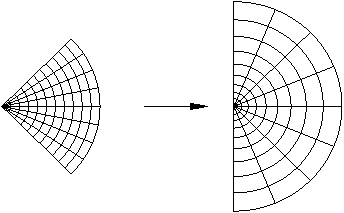
\includegraphics{figures/zsqplot}
\caption{What $z^2$ does to the sector
$\frac{-\pi}{2} \leq \operatorname{Arg} z \leq \frac{\pi}{2}$, $\sabs{z} <
1.1$.\label{fig:zsqplot}}
\end{myfig}

\begin{exbox}
\begin{exercise}
Prove that
\begin{exparts}
\item
If $\sabs{z}<1$, then $\lim\limits_{n\to \infty} z^n = 0$.
\item
If $\sabs{z}>1$, then $\lim\limits_{n\to \infty} z^n = \infty$.
\item
If $z \not= 1$ is such that $\sabs{z}=1$, then $z^n$ diverges as $n \to
\infty$.
\end{exparts}
\end{exercise}

\begin{exercise}[Easy]
On the unit circle parametrized by the angle $\theta$,
write $\sin(n\theta)$ and $\cos(n\theta)$ as a linear combination
of powers (including negative) of $z = e^{i\theta}$.
\end{exercise}
\end{exbox}

\subsection{Power series and radius of convergence}

A \emph{\myindex{power series}} around $p \in \C$ is simply the series
\begin{equation*}
\sum_{n=0}^\infty c_n {(z-p)}^n ,
\end{equation*}
where $c_n$ are some complex numbers.  Where it converges it defines a
function of $z$.  As the series clearly converges at $z=p$, we worry about
convergence at other points.  So we say the series is
\emph{convergent}\index{convergent power series}, if there is
some $z \not= p$ where the series converges.

The most important series, and in some sense the only one that we really
know how to sum, is the \emph{\myindex{geometric series}}.

\begin{prop}[Geometric series]
\leavevmode
\begin{enumerate}[(i)]
\item For $z \in \D$,
\begin{equation*}
\frac{1}{1-z} = \sum_{n=0}^\infty z^n .
\end{equation*}
\item For $z \not\in \D$,
\begin{equation*}
\sum_{n=0}^\infty z^n \quad \text{diverges.}
\end{equation*}
\item
Given $0 < r < 1$, then for all $z \in \overline{\Delta_r(0)}$
(that is, $\sabs{z} \leq r$)
\begin{equation*}
\abs{\frac{1}{1-z} - \sum_{n=0}^m z^n}
\leq \frac{r^{m+1}}{1-r} .
\end{equation*}
Consequently,
as $\frac{r^{m+1}}{1-r} \to 0$,
the geometric series converges uniformly
on $\overline{\Delta_r(0)}$.
\end{enumerate}
\end{prop}

\begin{proof}
All three items follow from
\begin{equation*}
1+z+z^2+\cdots+z^m = \frac{1-z^{m+1}}{1-z} ,
\end{equation*}
for all $z \not= 1$, which follows by summing 
$(1-z)(1+z+z^2+\cdots+z^m)$.  Details are left as an exercise.
\end{proof}

\begin{exbox}
\begin{exercise}
Fill in the details of the proof of the proposition above.  Do not forget
about the boundary of the disc.
\end{exercise}
\end{exbox}

A power series converges absolutely if the following series converges:
\begin{equation*}
\sum_{n=0}^\infty \sabs{c_n} \sabs{z-p}^n .
\end{equation*}
For $N < M$,
\begin{equation*}
\abs{\sum_{n=N+1}^M c_n {(z-p)}^n}
\leq
\sum_{n=N+1}^M \sabs{c_n} \sabs{z-p}^n.
\end{equation*}
Hence, if the sequence of partial sums of 
$\sum \sabs{c_n} \sabs{z-p}^n$ is Cauchy, so is the sequence
of partial sums of $\sum c_n {(z-p)}^n$.  Thus,
an absolutely convergent series
actually converges.

Let $r = \sabs{z-p}$, then we have the real series $\sum \sabs{c_n} r^n$.  Define
\begin{equation} \label{eq:rconvdef}
R = \frac{1}{\limsup\limits_{n \to \infty} \sqrt[n]{\sabs{c_n}}} ,
\end{equation}
where we interpret $\frac{1}{\infty} = 0$ and $\frac{1}{0} = \infty$,
so $R=\infty$ is allowed.

By the standard root test, the series $\sum \sabs{c_n} r^n$
converges if
\begin{equation*}
\limsup_{n \to \infty} \sqrt[n]{\sabs{c_n} r^n} = 
r \limsup_{n \to \infty} \sqrt[n]{\sabs{c_n}} = r \frac{1}{R} < 1 ,
\end{equation*}
and it diverges if $r \frac{1}{R} > 1$.  In other words,
the series converges if
$r < R$
and diverges if
$r > R$.  See \figureref{fig:radiusconvcomplex}.
We have proved the following proposition:

\begin{prop}[Cauchy--Hadamard theorem\footnote{%
Cauchy published this result in 1821, and Hadamard, despite also being
French, didn't know about it and published it in his thesis in 1888.}]
\index{Cauchy--Hadamard theorem}
A power series $\sum c_n {(z-p)}^n$ converges absolutely if
$\sabs{z-p} < R$ and diverges if
$\sabs{z-p} > R$, where $R$ is defined by \eqref{eq:rconvdef}.
\end{prop}

\begin{myfig}
\subimport*{figures/}{radiusconvcomplex.pdf_t}
\caption{Radius of convergence.\label{fig:radiusconvcomplex}}
\end{myfig}

The number $R$ is called the \emph{\myindex{radius of convergence}}.
The power series converges absolutely
in the disc $\Delta_R(p)$, and diverges
in the complement of the closure $\overline{\Delta_R(p)}$.
Convergence (or divergence) on the boundary circle $\partial \Delta_R(p)$
is a tricky matter.

A useful criterion for the radius of convergence is that the sequence
$\bigl\{ \sabs{c_n} r^n \bigr\}$ is
bounded whenever $0 < r < R$.

\begin{prop} \label{prop:cnrnbounded}
The series $\sum c_n {(z-p)}^n$ converges in $\Delta_{R}(p)$ for some
$R > 0$ if and only if
for every $r$ with
$0 < r < R$ there exists an $M > 0$ such that
\begin{equation*}
\sabs{c_n} \leq \frac{M}{r^n} \qquad \text{for all } n .
\end{equation*}
\end{prop}

It is not necessarily true that $\bigl\{ \sabs{c_n} R^n \bigr\}$
is bounded if $R$ is the radius of convergence.
For example, both $\sum z^n$ and $\sum n z^n$ have
radius of convergence 1 and the sequence of coefficients
is bounded in the first case and
not in the second.  However, $\{ n r^n \}$ is bounded for every $r < 1$.

\begin{proof}
Suppose the series converges in $\Delta_{R}(p)$ and
$0 < r < R$, then $\sum \sabs{c_n}r^n$ converges,
and the terms of that series are bounded.

Conversely, fix $r$, suppose 
$\sabs{c_n} r^n \leq M$ for all $n$, and suppose $0 < s < r$.
Then
\begin{equation*}
\sqrt[n]{\sabs{c_n} s^n}=
\frac{s}{r}\sqrt[n]{\sabs{c_n} r^n} \leq \frac{s}{r} \sqrt[n]{M} .
\end{equation*}
The limsup of the right hand side is strictly less than 1 as $\frac{s}{r} < 1$.
So the series converges absolutely in
$\overline{\Delta_s(p)}$.  As $s$ and $r$ with $0 < s < r < R$ were
arbitrary,
the series converges (absolutely) in $\Delta_R(p)$.
\end{proof}

The proof is farily typical for convergence results of power series.
Convergence in $\Delta_R(p)$, means boundedness of
$\{ \sabs{c_n} r^n \}$ in a smaller $\Delta_r(p)$, which only gets us convergence
in $\Delta_s(p)$.  See \figureref{fig:threediscs}.  But since $s$ and $r$
are arbitrary we get convergence everywhere.
\begin{myfig}
\subimport*{figures/}{threediscs.pdf_t}
\caption{The three discs from the convergence proof.\label{fig:threediscs}}
\end{myfig}

\begin{exbox}
\begin{exercise}
Prove the triangle inequality for series.  If $\sum_{n=0}^\infty c_n$
converges, then $\abs{\sum_{n=0}^\infty c_n} \leq \sum_{n=0}^\infty
\sabs{c_n}$ (possibly the right hand side is $\infty$).
\end{exercise}
\end{exbox}

The convergence inside the radius of convergence is even nicer than just absolute.
Let $K \subset \C$ be a set.
A power series $\sum c_n {(z-p)}^n$
\emph{\myindex{converges uniformly absolutely}}
\index{uniform absolute convergence}
for $z \in K$ when $\sum \sabs{c_n} \sabs{z-p}^n$
converges uniformly for $z \in K$.
Suppose a series converges uniformly absolutely.  It converges absolutely,
so it converges, and 
\begin{equation*}
\abs{
\sum_{n=0}^\infty c_n {(z-p)}^n
-
\sum_{n=0}^{m} c_n {(z-p)}^n
}
=
\abs{\sum_{n=m+1}^\infty c_n {(z-p)}^n} \leq
\sum_{n=m+1}^\infty \sabs{c_n} \sabs{z-p}^n .
\end{equation*}
The right hand side goes to zero uniformly in $z \in K$,
and so
a uniformly absolutely convergent series also converges
uniformly.  So the name fits the crime.

\begin{prop}
Let $\sum c_n {(z-p)}^n$ be a power series with radius of convergence $R
> 0$.  If $0 < r < R$, then the power series converges uniformly absolutely
in $\overline{\Delta_r(p)}$. Furthermore, let $U = \Delta_R(p)$ if $R < \infty$ and
$U = \C$ if $R=\infty$, and let $K \subset U$ be compact.
Then the series converges uniformly absolutely on $K$.
\end{prop}

In other words, power series converges uniformly (absolutely) on
compact subsets.

\begin{proof}
Without loss of generality suppose $R < \infty$.
Suppose $0 < r < R$.  As $\sum c_n {(z-p)}^n$ converges absolutely
on $\Delta_R(p)$, the series
$\sum \sabs{c_n} r^n$ converges (and in particular any tail of
that series converges).  Thus for $z \in \overline{\Delta_r(p)}$,
\begin{equation*}
\abs{
\sum_{n=0}^\infty \sabs{c_n} \sabs{z-p}^n
-
\sum_{n=0}^{m} \sabs{c_n} \sabs{z-p}^n
}
\leq
\sum_{n=m+1}^\infty \sabs{c_n} r^n .
\end{equation*}
The right hand side, which does not depend on $z$,
goes to zero as $m \to \infty$, and hence 
the series $\sum \sabs{c_n} \sabs{z-p}^n$ converges uniformly in $\overline{\Delta_r(p)}$.

If $K \subset \Delta_{R}(p)$ is compact, then there exists some $r <
R$ such that $K \subset \Delta_r(p)$ (consider an open cover of
$K$ by discs $\Delta_r(p)$ for all $r < R$).  The result follows.
\end{proof}

\begin{exbox}
\begin{exercise}
Show that the series $\sum_{n=1}^\infty \frac{1}{n^2} z^{n}$ has radius of
convergence $1$, and
show that it converges absolutely on the boundary of the unit disc.  Hence
it actually converges uniformly on the entire closed unit disc.
\end{exercise}

\begin{exercise}
Show that
$\sum_{n=0}^\infty n^n z^{n^n}$ has radius of convergence $1$,
while
$\sum_{n=0}^\infty n^n z^{n}$ is not convergent at all.
\end{exercise}

\begin{exercise}
Suppose
$\sum_{n=0}^\infty c_n z^{n}$ converges at $z=1$, but not absolutely.
Prove that the radius of convergence is 1.
\end{exercise}

\begin{exercise}
Suppose
$\sum_{n=0}^\infty a_n z^{n}$ and $\sum_{n=0}^\infty b_n z^{n}$
have a radius of convergence at least $r > 0$.  Show that
the sum series
$\sum_{n=0}^\infty (a_n+b_n) z^{n}$ has a radius of convergence at least
$r$ and converges to the sum of the two series.
\end{exercise}

\begin{exercise}
Given an $R > 1$, find two power series
$\sum_{n=0}^\infty a_n z^{n}$ and $\sum_{n=0}^\infty b_n z^{n}$,
such that both have radius of convergence exactly 1, but the 
sum
$\sum_{n=0}^\infty (a_n+b_n) z^{n}$ has a radius of convergence 
exactly $R$.  Hint: First figure out a series with radius of convergence
exactly $R$.
\end{exercise}

\begin{exercise}
Suppose
$\sum_{n=0}^\infty a_n z^{n}$ and $\sum_{n=0}^\infty b_n z^{n}$
have a radius of convergence at least $r > 0$.  Let 
$c_n = \sum_{k=0}^n a_{n-k}b_k$.  Show that
the series
$\sum_{n=0}^\infty c_n z^{n}$ has a radius of convergence at least
$r$ and converges to the product of the two series.
Hint: The key is to look at a point where both series converge absolutely,
then use the absolute convergence.
\end{exercise}
\end{exbox}

\begin{remark}
The last few exercises say that we can add and multiply series, however,
we won't need them later on as the two results are easy for holomorphic
functions, and we will show later that power series are
holomorphic and vice versa.  You should still try them, they are good
practice.
\end{remark}

%%%%%%%%%%%%%%%%%%%%%%%%%%%%%%%%%%%%%%%%%%%%%%%%%%%%%%%%%%%%%%%%%%%%%%%%%%%%%%

\section{Analytic functions}
\label{sec:analfuncs}

\subsection{Definition}

Functions that possess a convergent power series are called analytic.
From the beginnings of calculus until the 19\textsuperscript{th} century, 
when mathematicians considered a ``function'' they really meant
``analytic function'' (or something like it) in modern language.
One can talk about
both complex and real analytic functions depending on if the
variables are real or complex, and they may depend on one or several variables,
but we are interested in complex analytic functions of one variable. 
As there is little chance of confusion, we say just ``analytic'' instead of
``complex analytic.''

\begin{defn}
Let $U \subset \C$ be open.  A function $f \colon U \to \C$
is \emph{\myindex{analytic}}\index{complex analytic}
if for every $p \in U$, there exists 
an $r > 0$ and a
power series $\sum c_n {(z-p)}^n$ converging to $f$ on $\Delta_r(p) \subset
U \subset \C$.
\end{defn}

\begin{exbox}
\begin{exercise}[Easy]
Prove that polynomials $P(z)$ are analytic.
\end{exercise}

\begin{exercise}
Prove that $\frac{1}{z}$ is analytic in $\C \setminus \{ 0 \}$
by explicitly writing down 
a power series at any $p \in \C \setminus \{ 0 \}$
using the geometric series.
\end{exercise}
\end{exbox}

\subsection{Analytic functions are holomorphic}

Eventually, we will see that analytic functions and holomorphic functions are
one and the same.\footnote{%
For this reason, some authors define ``analytic'' to mean complex differentiable,
which is no problem eventually, but right now it would be.}
Let us start by proving that
analytic functions are holomorphic, that is, they are complex
differentiable.

\begin{prop}
Let $f \colon \Delta_R(p) \to \C$ be defined by
\begin{equation*}
f(z) = \sum_{n=0}^\infty c_n {(z-p)}^n ,
\end{equation*}
which converges in $\Delta_R(p)$.
Then $f$ is complex differentiable at every $z \in \Delta_R(p)$ and
\begin{equation*}
f'(z) = \sum_{n=1}^\infty n c_n {(z-p)}^{n-1} ,
\end{equation*}
which converges in $\Delta_R(p)$.
\end{prop}

\begin{proof}
Without loss of generality, let $p=0$.
Differentiate $z^n$ at $z_0$ by considering the difference
quotient
\begin{equation*}
\frac{z^n-z_0^n}{z-z_0}
=
\sum_{k=0}^{n-1}
z^k z_0^{n-1-k} ,
\end{equation*}
which goes to $n z_0^{n-1}$ as $z \to z_0$.
Apply the formula to $f$
term-wise.  If $z_0$ and $z$ are in $\Delta_R(0)$, then
\begin{equation*}
\frac{f(z) - f(z_0)}{z-z_0}
=
\sum_{n=1}^\infty c_n \frac{z^n-z_0^n}{z-z_0}
=
\sum_{n=1}^\infty c_n \sum_{k=0}^{n-1} z^k z_0^{n-1-k} .
\end{equation*}
The right hand side is defined even if $z_0 = z$.
We must show that the expression above is continuous as a function of $z$
at $z_0$.
It is continuous provided that the series above
%(the series whose terms are $c_n z_0^k z^{n-1-k}$)
converges uniformly for $z$ in a
neighborhood of $z_0$.

The setup will be just like in \figureref{fig:threediscs}.
Let $r$ and $s$ be such that $0 < s < r < R$ and suppose that $z_0$ and $z$ are
in $\Delta_s(0)$.
\begin{equation*}
%\abs{c_n \frac{z^n-z_0^n}{z-z_0}}
%=
\abs{c_n \sum_{k=0}^{n-1} z^k z_0^{n-1-k}}
\leq
\sum_{k=0}^{n-1} 
\sabs{c_n} s^{n-1}
=
n
\sabs{c_n} s^{n-1}
=
n
\sabs{c_n} r^{n-1} {\left(\frac{s}{r}\right)}^{n-1} .
\end{equation*}
The expression
$\sabs{c_n} r^{n-1}$ is bounded by some $M > 0$ because the series for $f$ converges
in $\Delta_R(0)$ and $r < R$.
As
\begin{equation*}
\sqrt[n]{
n \sabs{c_n} s^{n-1}
}
=
\sqrt[n]{
n \sabs{c_n} r^{n-1} {\left(\frac{s}{r}\right)}^{n-1}
}
\leq
\sqrt[n]{
n M {\left(\frac{s}{r}\right)}^{n-1}
}
\quad\underset{\text{as } n \to \infty}{\to}\quad
\frac{s}{r} < 1 ,
\end{equation*}
the root test shows that
%\begin{equation*}
%\sum_{n=1}^\infty n \sabs{c_n} r^{n-1} {\left(\frac{s}{r}\right)}^{n-1}
%\end{equation*}
$\sum n \sabs{c_n} s^{n-1}$
converges.
So the series for the difference quotient,
\begin{equation*}
\sum_{n=1}^\infty c_n \sum_{k=0}^{n-1} z^k z_0^{n-1-k} ,
\end{equation*}
converges uniformly in $z$ on $\Delta_s(p)$, and
we can swap the limit $z \to z_0$ with the series limit:
\begin{equation*}
\lim_{z \to z_0}
\frac{f(z)-f(z_0)}{z-z_0}
=
\sum_{n=1}^\infty c_n \sum_{k=0}^{n-1} z_0^k z_0^{n-1-k}
=
\sum_{n=1}^\infty n c_n z_0^{n-1} .
\end{equation*}
As $s$ and $r$ were arbitrary, the convergence happens in all of
$\Delta_R(0)$.
\end{proof}

The derivative is again given by a power series.
By induction, it follows that a power series is infinitely complex
differentiable.

\begin{cor} \label{cor:convpowserinfdif}
Let $f \colon \Delta_R(p) \to \C$ be defined by a convergent power series
\begin{equation*}
f(z) = \sum_{n=0}^\infty c_n {(z-p)}^n .
\end{equation*}
Then $f$ is infinitely complex differentiable in $\Delta_R(p)$,
and the $k$\textsuperscript{th} derivative is given by
\begin{equation*}
f^{(k)}(z) = \sum_{n=k}^\infty n(n-1)\cdots(n-k+1) c_n {(z-p)}^{n-k} ,
\end{equation*}
which converges in $\Delta_R(p)$.
Furthermore,
\begin{equation*}
c_n =
\frac{f^{(n)}(p)}{n!} .
\end{equation*}
\end{cor}

\begin{exbox}
\begin{exercise}
Fill in the details of the proof of the corollary.
\end{exercise}
\end{exbox}

An important consequence of this corollary that should be
emphasized is that if $f$ is given by the convergent power series in
$\Delta_R(p)$ as above, then the power series is unique.  This conclusion
follows from the formula for the coefficients $c_n$.  In fact, the
coefficients depend only on the values of $f$ in an arbitrarily small
neighborhood of $p$.

If we apply the corollary to analytic functions at every point,
we find that they are infinitely differentiable:

\begin{cor} \label{cor:analinfdif}
An analytic function is infinitely complex differentiable, and each
derivative is analytic.
\end{cor}

\begin{remark}
A subtle issue is that while we proved that analytic functions are
complex differentiable because they have a power series representation,
we did not yet prove that a convergent power series defines an analytic
function.  What is left is to prove that a power series convergent
in $\Delta_R(p)$ can be
expanded about a different point in $\Delta_R(p)$.  That will follow
once we prove that holomorphic functions are analytic.
\end{remark}

\begin{exbox}
\begin{exercise}
Suppose $f \colon \Delta_R(0) \to \C$ is given by a convergent power
series
$f(z) = \sum_{n=0}^\infty c_n z^n$.
Suppose that for some $\epsilon > 0$, $f(x) = 0$ for all $x \in
(-\epsilon,\epsilon)$ (an interval on the real line).
Using the corollary,
prove that $c_n = 0$ for all $n$ and hence $f$ is identically zero.
\end{exercise}

\begin{exercise} \label{exercise:antiderseries}
Suppose $f \colon \Delta_R(p) \to \C$ is given by a convergent power
series
$f(z) = \sum_{n=0}^\infty c_n {(z-p)}^n$.
Antidifferentiate:
Show that there exists a power series converging in $\Delta_R(p)$
whose complex derivative is $f(z)$.
\end{exercise}

\begin{exercise} 
Suppose $f \colon \Delta_R(0) \to \C$ is given by a convergent power
series
$f(z) = \sum_{n=0}^\infty c_n {z}^n$ and $R > 1$.
Show that there is an $M>0$ such that
$\sabs{f^{(n)}(0)} \leq n! M$ for all $n$.
\end{exercise}
\end{exbox}

\subsection{The exponential}

We met the complex exponential $e^z$ before
(\subsectionref{subsection:firstdefexp}), and we proved
that it is holomorphic and its own derivative
(\exerciseref{exercise:exponentialholomorphic}).  We can now see this fact
from a different vantage point.\footnote{%
That vantage point being the same as that dark place in your past
that is the undergraduate differential equations class when you covered
power series methods for solving ODEs.}
We claim we could have defined the exponential
using a power series.

\begin{prop}
The power series
\begin{equation*}
f(z) = \sum_{n=0}^\infty \frac{1}{n!} z^n ,
\end{equation*}
is the unique convergent power series at the origin
such that $f(0)=1$ and $f'=f$.
Moreover, the series converges on $\C$ and
$f(z) = e^z$.
\end{prop}

\begin{proof}
It is not hard to check directly (exercise)
that the series converges in all of $\C$.
And we now know that it is holomorphic and how to take its complex derivative.

Let $f$ be a convergent power series at the origin
\begin{equation*}
f(z) = \sum_{n=0}^\infty c_n z^n ,
\end{equation*}
and suppose $f(0)=1$ and $f'=f$.
Obviously, $f(0)=1$ implies that $c_0 = 1$.
The trick is to figure out the rest of the series.
We now know how to
differentiate such a series, we just do it term-by-term, ``formally.''
So
\begin{equation*}
f'(z) =
\sum_{n=1}^\infty n c_n z^{n-1} =
\sum_{n=0}^\infty (n+1) c_{n+1} z^{n} .
\end{equation*}
As the coefficients of the power series at zero are unique, we get
$c_n = (n+1) c_{n+1}$.  By induction we see that $c_n = \frac{1}{n!}$.

Let's prove that $f$ is the exponential.  Both functions are
holomorphic, the exponential is never zero, and both are equal to their
derivatives.  So,
\begin{equation*}
\frac{d}{dz} \left[ \frac{f(z)}{\exp(z)} \right]
=
\frac{f'(z)\exp(z) - f(z) \exp'(z)}{{\bigl(\exp(z)\bigr)}^2}
=
\frac{f(z)\exp(z) - f(z) \exp(z)}{{\bigl(\exp(z)\bigr)}^2}
= 0.
\end{equation*}
So, $f(z) = C \exp(z)$ for some constant (\propref{prop:zeroder}).
As $f(0) = \exp(0) = 1$,
we conclude $C=1$.
\end{proof}

\begin{exbox}
\begin{exercise}
Prove that the series for the exponential above converges by computing
the radius of convergence directly
(e.g. show that the series converges for every $z \in \C$).
\end{exercise}

\begin{exercise}
Compute the series for $\sin z$ and $\cos z$, then show that these satisfy
$f''(z) = -f(z)$.
\end{exercise}

\begin{exercise}
Show that there exists a holomorphic $f \colon \C \to \C$ that
solves $f'(z) + z f(z) = 0$ and such that $f(0) = 1$.  Hint: Solve formally
as a power series,
then see if you can guess the answer in ``closed form,'' that is, in terms
of the exponential.  Hint \#2: What is $f'(0)$?
\end{exercise}

\begin{exercise}
For any $a,b \in \C$, show that there exists a holomorphic $f \colon \C \to
\C$ such that $f''(z) = z f(z)$, and $f(0) = a$ and $f'(0) = b$.
Hint: Define formally and show convergence.
Note: These are the \emph{\myindex{Airy functions}}, and they have some
interesting behavior; on the real line they oscillate like sine and cosine
for negative $z$ and behave like an exponential for positive $z$.
\end{exercise}
\end{exbox}

\subsection{The identity theorem}

One of the main properties of analytic functions is that once you know them
in a neighborhood you know them everywhere.  In fact, a much more general
statement is true; you only need to know an analytic function on a set with
a limit point.

\begin{thm}[Identity]\index{identity theorem!holomorphic functions}%
\label{thm:identity}
Suppose $U \subset \C$ is a domain, 
and $f \colon U \to \C$ analytic.
If $Z_f = \bigl\{ z \in U : f(z) = 0 \bigr\}$
has a limit point in $U$, then $f$ is identically zero.
In other words, all points of $Z_f$ are isolated unless $f \equiv 0$.
\end{thm}

\begin{defn}
The points in the set $Z_f$ are called the \emph{zeros}\index{zero} of $f$.
\end{defn}

The first common application of this theorem is that the zeros of
nonconstant functions are isolated.  That is, if $f(p)=0$, but $f$ is not
identically zero, then there is a disc $\Delta_r(p)$ such that $f(z) \not=
0$ for all $z \in \Delta_r(p) \setminus \{ 0 \}$.

Another common application of the theorem is the following weaker statement:
``If the function is zero on a nonempty open subset, then $f \equiv 0$.''

\begin{proof}
Suppose $f$ is not identically zero.
The set $Z_f$ is closed as $f$ is continuous.  So we have to show
that points of $Z_f$ are isolated.
Without loss of generality suppose that $0 \in U$ and $0 \in Z_f$,
and suppose $0$ is not in the interior of $Z_f$.
Write $f$ near $0$ as
\begin{equation*}
f(z) = \sum_{n=0}^\infty c_n z^n .
\end{equation*}
As $f(0) = 0$, $c_0 =0$.  Let $k$ be the first $k$ such that $c_k \not=0$,
such a $k$ exists as otherwise $f$ would be identically zero near $0$
and we assumed $0$ is not in the interior of $Z_f$.  Then
\begin{equation*}
f(z) = z^k \sum_{n=k}^\infty c_n z^{n-k} = z^k g(z) .
\end{equation*}
The series $g(z)$ above is a convergent power series and $g(0) = c_k \not=
0$.  A power series is continuous, and hence $g(z) \not= 0$ near $0$.
As $z^k$ is only zero at $0$, we find that $0$ is an isolated zero of $f$.

So the only points of $Z_f$ that are not isolated are those that are in the
interior of $Z_f$.  Let $Z_f' \subset Z_f$ be the set of nonisolated points
of $Z_f$.  This set must be closed as $Z_f$ is closed, and no sequence
of points in $Z_f'$ can
got to an isolated point of $Z_f$.  We have proved above that nonisolated
points must be interior points of $Z_f$ (and hence of $Z_f'$).
So $Z_f'$ is both open and closed.  As $U$ is connected and 
that $Z_f' \not= U$, we conclude $Z_f' = \emptyset$.
Thus all points of $Z_f$ are isolated.
\end{proof}

\begin{exbox}
\begin{exercise}
Suppose $U \subset \C$ is a domain and $f \colon U \to \C$ and $g \colon U \to
\C$ are
analytic such that the set $\{ z \in U : f(z) = g(z) \}$ has a limit
point in $U$.  Prove that $f = g$ everywhere.
\end{exercise}

\begin{exercise}
Suppose $U \subset \C$ is a domain and $f \colon U \to \C$ and $g \colon U \to
\C$ are analytic such that $f(z)g(z) = 0$ for all $z \in U$.
Prove that either $f$ or $g$ is identically zero.
(In other words, the ring of holomorphic functions on $U$ is an integral
domain.)
\end{exercise}

\begin{exercise}
Suppose $U \subset \C$ is a domain and $f \colon U \to \C$ is
analytic and not constant.  Show that if $K \subset U$ is compact
then $Z_f \cap K$ is finite.
\end{exercise}
\end{exbox}

Think of the implications.  If $f \colon U \to \C$ is analytic, and we know
$f$ in a tiny disc $\Delta_r(p)$ for an arbitrarily small $r$, then
we know $f$ on all of $U$.

\begin{exbox}
\begin{exercise}
Suppose $U \subset \C$ is a domain and $f \colon U \to \C$ and $g \colon U \to
\C$ are analytic, and $p \in U$.  Suppose that $f^{(k)}(p) = g^{(k)}(p)$
for $k=0,1,2,\ldots$.  Prove that $f = g$ everywhere.
\end{exercise}

\begin{exercise}
Suppose $U \subset \C$ is a domain and $f \colon U \to \C$ is analytic.
Prove that if $f'(z) = 0$ for
all $z \in U$ in a neighborhood of some $z_0 \in U$, then $f$ is constant.
\end{exercise}

\begin{exercise}
Suppose $U \subset \C$ is a domain, $a, b, c \in \C$, $z_0 \in U$, show that
an analytic solution $f$ on $U$ to a linear equation $f'(z) = a f(z) + b$
given $f(z_0) = c$ is unique if it exists.
\end{exercise}
\end{exbox}

One of the downsides of analytic functions is that there are no compactly
supported analytic functions on $\C$.  The \emph{\myindex{support}}
of a function $f \colon U
\to \C$ is the closure (in $U$) of the set
$\bigl\{ z \in U : f(z) \not= 0 \bigr\}$, that is, 
the support is $\overline{U \setminus Z_f} \cap U$.

\begin{exbox}
\begin{exercise}
Let $U \subset \C$ be a domain and $f \colon U \to \C$ is analytic and
is not identically zero.
Show that the support of $f$ is $U$.
In particular, the support cannot be compact.
\end{exercise}
\end{exbox}



%%%%%%%%%%%%%%%%%%%%%%%%%%%%%%%%%%%%%%%%%%%%%%%%%%%%%%%%%%%%%%%%%%%%%%%%%%%%%%
%%%%%%%%%%%%%%%%%%%%%%%%%%%%%%%%%%%%%%%%%%%%%%%%%%%%%%%%%%%%%%%%%%%%%%%%%%%%%%
%%%%%%%%%%%%%%%%%%%%%%%%%%%%%%%%%%%%%%%%%%%%%%%%%%%%%%%%%%%%%%%%%%%%%%%%%%%%%%

\chapter{Line Integrals and Rudimentary Cauchy Theorems} \label{ch:cauchysimple}

\begin{myquote}
The Brain: Pinky, are you pondering what I am pondering?

Pinky:  Uh, I think so, Brain, but we'll never get a monkey to use dental floss.
\end{myquote}

%%%%%%%%%%%%%%%%%%%%%%%%%%%%%%%%%%%%%%%%%%%%%%%%%%%%%%%%%%%%%%%%%%%%%%%%%%%%%%

\section{Line integrals}
\label{sec:lineints}

\subsection{Paths}

\begin{defn}
\glsadd{not:contdifffuncs}%
A \emph{\myindex{piecewise $C^1$ path}} or a \emph{\myindex{path}} for short
is
a continuous complex-valued piecewise continuously
differentiable (piecewise $C^1$) function $\gamma \colon [a,b] \to \C$ 
such that $\gamma'(t)$ and all its one sided limits are never
0.\footnote{Some authors do not require the derivative not being zero, and
in fact in the way that we use the paths, the requirement is not crucial,
but leaving it off does lead to allowing some strange paths.}
\end{defn}

All of our paths will be piecewise $C^1$, so we may forget to mention it
sometime.
By ``piecewise $C^1$,''
we mean that there exist numbers $t_0 = a < t_1 < \cdots
< t_k = b$ for some $k$ such that $\gamma|_{[t_{\ell-1},t_\ell]}$ is
continuously differentiable ($C^1$) up to
the boundary for every $\ell$ and its derivative is never zero.
In other words, $\gamma$ is continuously differentiable inside all the
subintervals $(t_{\ell-1},t_\ell)$ and the one sided limits
\begin{equation*}
\lim_{t \uparrow t_\ell} \gamma'(t) \qquad
\lim_{t \downarrow t_\ell} \gamma'(t)
\end{equation*}
exist for all $\ell$ (except of course only one exists at $a$ or $b$),
and these limits are nonzero.
Another way to say it is that $\gamma'(t)$ extends to a nonzero
continuous function on each closed interval $[t_{\ell-1},t_{\ell}]$.
Allowing these ``corners'' makes working with path easier
as we can define them easily piece-wise, and finitely many corners like
this will make no difference on the calculations.
Do note also that we are saying that paths are continuous.  We will allow
discontinuities just a little later with ``chains.''

When we say that $\gamma$ is a path in $U \subset \C$\index{path in $U$},
we mean that
$\gamma \colon [a,b] \to U$ is a path.  Another common abuse of language we
will freely and shamelessly commit is that if we refer to $\gamma$
as if it were a set we mean the image $\gamma\bigl([a,b]\bigr)$.
Nowhere will we really use or need that $\gamma'$ is never zero,
but leaving that off would allow some paths that one would generally not
wish to call piecewise $C^1$,
as you will see in the exercises.

\begin{example}
The path $\gamma \colon [0,4] \to \C$, given by
\begin{equation*}
\gamma(t) =
\begin{cases}
t          & \text{if } t \in [0,1],\\
1 + i(t-1) & \text{if } t \in (1,2],\\
3-t + i    & \text{if } t \in (2,3],\\
i(4-t)     & \text{if } t \in (3,4],
\end{cases}
\end{equation*}
is a piecewise $C^1$ path traversing the sides unit square.
See \figureref{fig:squarepath}.  You should check that the
conditions are satisfied.  For example, 
on $t \in (0,1)$, $\gamma'(t) = 1$, and so
$\lim_{t \uparrow 1} \gamma'(t) = 1$.  Similarly
$\lim_{t \downarrow 1} \gamma'(t) = i$, and so on.
\begin{myfig}
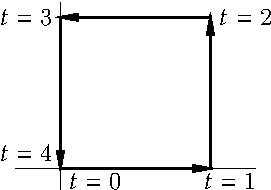
\includegraphics{figures/squarepath}
\caption{The path $\gamma$ traversing the unit square.\label{fig:squarepath}}
\end{myfig}
\end{example}

\subsection{The line integral}

\begin{defn}
Given a piecewise $C^1$ path $\gamma \colon [a,b] \to \C$ and a continuous
function $f$ defined on 
$\gamma$, 
we define the \emph{\myindex{line integral}}\footnote{%
This integral is also called
a \emph{\myindex{path integral}}, 
a \emph{\myindex{curve integral}}, or
a \emph{\myindex{contour integral}}.}
\glsadd{not:pathint}%
\begin{equation*}
\int_{\gamma} f(z) \, dz
\overset{\text{def}}{=}
\int_a^b f\bigl(\gamma(t)\bigr) \gamma'(t) \, dt .
\end{equation*}
\end{defn}

The definition makes sense despite $\gamma'(t)$ not existing at possibly
finitely many points.  The integrand is undefined
at finitely many points but is piecewise continuous, and this is enough
to be Riemann integrable: On each closed interval
$[t_{\ell-1},t_\ell]$, the integrand extends to a continuous
function of the whole closed integral.

Let us compute the most important example of a line integral.

\begin{example} \label{example:integralpowerz}
Let $\gamma \colon [0,2\pi] \to \C$ given by $\gamma(t) = r e^{it}$ be
the circle of radius $r$ oriented counterclockwise,
that is, $\partial \Delta_r(0)$.  See \figureref{fig:circlepath}.
For $n \in \Z$, we claim that
\begin{equation*}
\int_\gamma z^n \, dz
=
\begin{cases}
2\pi i & \text{if } n=-1, \\
0 & \text{otherwise.}
\end{cases}
\end{equation*}

\begin{myfig}
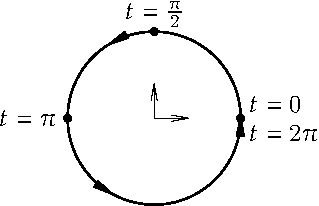
\includegraphics{figures/circlepath}
\caption{The path $\gamma$ traversing the circle.\label{fig:circlepath}}
\end{myfig}

First, $\gamma'(t) = i r e^{it}$.
To prove the claim we compute
\begin{equation*}
\int_\gamma z^n \, dz
=
\int_0^{2\pi}
r^n
e^{int} i r e^{it} \, dt
=
i r^{n+1}
\int_0^{2\pi}
e^{i(n+1)t} \, dt .
\end{equation*}
The result follows as the integral on the right hand side above is zero
(write it in terms of sines and cosines, exercise below) unless $n+1 = 0$,
in which case, the integral 
is $2\pi$ and $r^{n+1} = 1$.  Note in particular that the value of the
integral does not depend on $r$.
\end{example}

\begin{exbox}
\begin{exercise}
Prove that if $k\not= 0$ then $\int_0^{2\pi} e^{ik t} \, dt = 0$.
\end{exercise}

\begin{exercise}
Compute $\int_\gamma \bar{z}^n \, dz$ for all $n \in \Z$ and $\gamma$ as in
\exampleref{example:integralpowerz}.
\end{exercise}
\end{exbox}

Our line integral definition above is equivalent to the definition you
have seen in multivariable calculus.  Actually it is a special case of it.
Let $\gamma(t) = \bigl( x(t), y(t) \bigr)$, for $t \in [a,b]$, be a path,
and let $dz = dx + i\, dy$.
Then
\begin{equation*}
\begin{split}
\int_{\gamma} f(z) \, dz
& =
\int_{\gamma} f(z) \, (dx + i\, dy)
\\
& =
\int_{\gamma} f(z) \, dx + i f(z) \, dy
=
\int_a^b \bigl( f(z) x'(t) + i f(z) y'(t) \bigr) \, dt .
\end{split}
\end{equation*}
In the second line you should recognize the definition of a line integral
$\int_\gamma P\,dx + Q \, dy$ from calculus.  An arbitrary
line integral in the plane can be obtained if we also include $d\bar{z}$.  See the
exercise below.

\begin{exbox}
\begin{exercise} \label{exercise:realpathintegral}
\glsadd{not:dz}\glsadd{not:dzbar}%
Let $dz = dx + i \, dy$ and 
$d\bar{z} = dx - i \, dy$.  Show that for every (real- or complex-valued) continuous $P$ and $Q$,
there exist continuous (complex-valued) $F$ and $G$ such that
\begin{equation*}
\int_{\gamma} P \, dx + Q \, dy
=
\int_{\gamma} F \, dz + G \, d\bar{z} .
\end{equation*}
%Namely, the line integral we defined is just the $dz$ part of
%the general line integral in $\R^2$.
Then show that any path integral
can be computed if you only know how to compute integrals of the form $\int_\gamma f(z) \, dz$.
\end{exercise}
\end{exbox}

The value of the integral does not depend on how we parametrize the image of
the path, except it does depend on orientation.  It is easy to see why if
$\gamma \colon [a,b] \to \C$ is continuously differentiable and we have
an increasing continuously differentiable $h \colon [c,d] \to [a,b]$ such
that $h(c)=a$ and $h(d) = b$.  Then $\gamma \circ h$ is a new
smooth path that is a different parametrization of $\gamma$.
Change of variable $t=h(s)$ from calculus then says
\begin{equation*}
\begin{split}
\int_{\gamma} f(z) \, dz
& =
\int_a^b f\bigl( \gamma(t) \bigr) \gamma'(t) \, dt
\\
& =
\int_c^d f\Bigl( \gamma\bigl(h(s)\bigr) \Bigr) \gamma'\bigl(h(s)\bigr) h'(s) \, ds
=
\int_{\gamma \circ h} f(z) \, dz.
\end{split}
\end{equation*}
If, on the other hand, $h$ is decreasing and $h(c)=b$ and $h(d)=a$, then the
sign changes in the change of variables and
\begin{equation*}
\int_{\gamma} f(z) \, dz =
- \int_{\gamma \circ h} f(z) \, dz.
\end{equation*}

The general version of this result, a version of which we state below,
is a bit more difficult to prove.
As this result, while
morally important, is actually more of a technicality so that we only have
to refer to the image rather than the actual path parametrization, we will
leave its proof as an exercise.

\begin{prop}[Reparametrization]\index{reparametrization of paths}%
Suppose $\gamma \colon [a,b] \to \C$ and $\alpha \colon [c,d] \to \C$ are
piecewise $C^1$ paths such that
$\gamma\bigl([a,b]\bigr) = \alpha\bigl([c,d]\bigr)$.
Suppose either
\begin{enumerate}[(i)]
\item
$\gamma$ and $\alpha$ are injective, or
\item
$\gamma|_{(a,b]}$ and
$\alpha|_{(c,d]}$ are injective and 
$\gamma(a)=\alpha(c)=\gamma(b)=\alpha(d)$.
\end{enumerate}
Then there exists a strictly monotone continuous $h \colon [c,d] \to [a,b]$ such
that $\gamma\bigl(h(t)\bigr) = \alpha(t)$ for all $t \in [c,d]$.
\begin{enumerate}[(i)]
\item
If $h$ is increasing, then for every $f$ continuous on the path,
\begin{equation*}
\int_\gamma f(z) \, dz = \int_{\alpha} f(z) \, dz .
\end{equation*}
\item
If $h$ is decreasing, then for every $f$ continuous on the path,
\begin{equation*}
\int_\gamma f(z) \, dz = - \int_{\alpha} f(z) \, dz .
\end{equation*}
\end{enumerate}
\end{prop}

\begin{exbox}
\begin{exercise}
Prove the first case of the reparametrization proposition, that is,
suppose $\gamma$ and $\alpha$ are injective.
\begin{exparts}
\item
Prove the existence of $h$, its monotonicity, and continuity.
Hint: First prove $\gamma^{-1}$ is a continuous function on
$\gamma\bigl([a,b]\bigr)$ using that closed subsets of $[a,b]$
are compact.
\item
Prove in the case when $f=1$.
Hint: fundamental theorem of calculus.
\item
Prove the proposition for any continuous $f$.
Hint: Cut the path into small pieces where
you can approximate $f$ by a constant and apply the
last part.
\end{exparts}
\end{exercise}

\begin{exercise}
Prove the second case of thereparametrization for closed paths,
assuming only that $\gamma|_{(a,b]}$ and
$\alpha|_{(c,d]}$ are injective and
$\gamma(a)=\alpha(c)=\gamma(b)=\alpha(d)$.
\end{exercise}

\begin{exercise}
Any piecewise $C^1$ path $\gamma \colon [a,b] \to \C$
can be reparametrized to a $C^1$ ``path'' as long as the derivative
is allowed to vanish at some points.
That is, there exists a strictly increasing
continuous $h \colon [a,b] \to [a,b]$ such that
$\gamma \circ h$ is $C^1$.
Hint: Make the derivative at the ``corners'' zero.
\end{exercise}

\begin{exercise}[Tricky]
Consider infinitely many nested circles all touching at one point
and let that point be the origin: Suppose $r_n$ be the radius of the
$n$\textsuperscript{th}
circle and the $n$\textsuperscript{th} circle is given by $r_n e^{i(-1)^n\theta} - r_n$, for $0 \leq
\theta \leq 2\pi$ (they are traversed in alternating directions).
If $\sum r_n < \infty$, then you can find a continuous
$C^1$ function $\gamma \colon
[0,1] \to \C$ that traverses all the circles.  If $\sum r_n = \infty$, then
you can find a continuous $\gamma \colon [0,1] \to \C$ that is $C^1$ on
$(0,1]$, but necessarily $\lim_{t \to 0} \gamma'(t)$ does not exist.
\end{exercise}
\end{exbox}

\begin{remark}
The last two exercises show why we must morally
require that $\gamma'(t)$ never vanishes (including the one sided limits)
for piecewise $C^1$ paths.
We thinking of the path
as the set
$\gamma\bigl([a,b]\bigr)$,
not the parametrization, and where the path is $C^1$
we want it to not have ``corners.''
In practical terms, we won't really use that the derivative never vanishes,
but we lose nothing of real value by the extra requirement.
\end{remark}

Due to the reparametrization result above,
we often write down the ``boundary'' of a certain open set
(as long as that boundary is piecewise $C^1$ of course)
and consider any parametrization going counterclockwise
when integrating it, without explicitly giving the parametrization.
For example, given a disc $\Delta_r(p)$, we parametrize
the boundary $\partial \Delta_r(p)$ by
$\gamma  \colon [0,2\pi] \to \C$ given by $\gamma(t) = p +
re^{it}$, and then we write
\begin{equation*}
\int_{\partial \Delta_r(p)} f(z) \, dz
=
\int_{\gamma} f(z) \, dz .
\end{equation*}
This equality could be simply taken as a definition of integration over
$\partial \Delta_r(p)$.

A version of reparametrization is the following ``$u$-substitution'' type of
result.

\begin{prop} \label{prop:usubst}
Let $U,V \subset \C$ be open sets, $\gamma \colon [a,b] \to V$ be a piecewise
$C^1$ path, $h \colon V \to U$ be holomorphic, and $f \colon U \to \C$
is continuous.  Then $h \circ \gamma$ is a piecewise $C^1$ path in $V$ and
\begin{equation*}
\int_{\gamma} f\bigl(h(z)\bigr) h'(z) \, dz
=
\int_{h \circ \gamma} f(w) \, dw .
\end{equation*}
\end{prop}

\begin{proof}
That $h \circ \gamma$ is a piecewise $C^1$ path is obvious.  To prove the
equality we just parametrize and apply the chain rule, in particular
$(h \circ \gamma)'(t) = h'\bigl(\gamma(t)\bigr) \gamma'(t)$:
\begin{multline*}
\int_{\gamma} f\bigl(h(z)\bigr) h'(z) \, dz
=
\int_a^b
f\Bigl(h\bigl(\gamma(t)\bigr)\Bigr) h'\bigl(\gamma(t)\bigr) \gamma'(t) \, dt
\\
=
\int_a^b
f\bigl((h \circ \gamma)(t)\bigr) (h \circ \gamma)'(t) \, dt
=
\int_{h \circ \gamma} f(w) \, dw . \qedhere
\end{multline*}
\end{proof}

\begin{exbox}
\begin{exercise}
Let $f \colon \partial \D \to \C$ be a continuous function.  Prove that
\begin{equation*}
\int_{\partial \D} f(z) \, dz
=
\int_{\partial \D} \frac{f\bigl(\frac{1}{z}\bigr)}{z^2} \, dz
=
\int_{\partial \D} f(\bar{z}) \bar{z}^2 \, dz .
\end{equation*}
\end{exercise}
\end{exbox}

\subsection{Arclength integral}

We can also integrate with respect to arclength, the $ds$ from calculus.
We will write $ds$ as $\sabs{dz}$.  That is, for an $f$ continuous on
a piecewise $C^1$ path $\gamma \colon [a,b] \to \C$,
we define
\glsadd{not:arclength}
\begin{equation*}
\int_\gamma f(z) \, \sabs{dz}
\overset{\text{def}}{=}
\int_a^b f\bigl( \gamma(t) \bigr) \sabs{\gamma'(t)} \, dt .
\end{equation*}

With this definition we can do some estimates on line integrals.

\begin{prop}[Triangle inequality for line integrals]%
\index{triangle inequality!line integrals}
Suppose $\gamma \colon [a,b] \to \C$ is 
a piecewise $C^1$ path and $f$ is a continuous function on
$\gamma$.  Then
\begin{equation*}
\abs{\int_\gamma f(z) \, dz} \leq \int_\gamma \sabs{f(z)} \, \sabs{dz} .
\end{equation*}
In particular, if $\sabs{f(z)} \leq M$ on $\gamma$ and $\ell = \int_\gamma ds
= \int_{\gamma} \sabs{dz}$ is the length of $\gamma$, then
\begin{equation*}
\abs{\int_\gamma f(z) \, dz} \leq M \ell .
\end{equation*}
\end{prop} 

\begin{proof}
We estimate using \propref{prop:inttriangleineq},
\begin{equation*}
\abs{\int_\gamma f(z) \, dz}
=
\abs{\int_a^b f\bigl( \gamma(t) \bigr) \gamma'(t) \, dt}
\leq
\int_a^b \abs{ f\bigl( \gamma(t) \bigr) }  \sabs{ \gamma'(t) } \, dt
\leq
M
\int_a^b \sabs{ \gamma'(t) } \, dt .
\qedhere
\end{equation*}
\end{proof}

Arclength is not preserved under uniform convergence of the paths.
In other words, just because the images of two paths are very close to each
other, does not mean that the integrals over them will be the same.
So one has to be careful when saying that two paths are close to each other.  You
would need that the derivatives are close as well.

\begin{exbox}
\begin{exercise}
\begin{exparts}
\item
Find a sequence of piecewise $C^1$ paths $\gamma_n \colon [0,1] \to \C$
that uniformly converge to a constant function (one could say a path of
length zero), but such that $\int_{\gamma_n} \sabs{dz} \geq n$.
\item
Suppose a sequence of $C^1$ paths $\gamma_n \colon [0,1] \to \C$
converges uniformly to a $C^1$ path $\gamma \colon [0,1] \to \C$
such that $\gamma_n'$ converges uniformly to $\gamma'$, then
$\int_{\gamma_n} \sabs{dz} \to
\int_{\gamma} \sabs{dz}$.
\end{exparts}
\end{exercise}
\end{exbox}

\subsection{Chains}

It is useful to combine paths; to have a certain ``arithmetic'' of paths.
The resulting objects are called \emph{chains}, and they
are just formal combinations of paths.  For example, if $\gamma$
and $\alpha$ are piecewise $C^1$ paths, then the chain  $\gamma+\alpha$
is an object over which we can integrate functions that are continuous
on the image of both:
\begin{equation*}
\int_{\gamma + \alpha} f(z) \, dz
\overset{\text{def}}{=}
\int_{\gamma} f(z) \, dz +
\int_{\alpha} f(z) \, dz .
\end{equation*}

\begin{defn}
A \emph{\myindex{chain}} in $U \subset \C$ is an expression
\begin{equation*}
\Gamma = a_1 \gamma_1 + \cdots + a_n \gamma_n ,
\end{equation*}
where $a_1,\ldots,a_n \in \Z$ and $\gamma_1,\ldots,\gamma_n$
are piecewise $C^1$ paths in $U$.  We integrate over $\Gamma$ as
\begin{equation*}
\int_{\Gamma} f(z) \, dz
=
\int_{a_1 \gamma_1 + \cdots + a_n \gamma_n} f(z) \, dz
\overset{\text{def}}{=}
a_1 \int_{\gamma_1} f(z) \, dz +
\cdots
+
a_n \int_{\gamma_n} f(z) \, dz .
\end{equation*}
Two chains $\Gamma_1$ and $\Gamma_2$ in 
$U$ are
\emph{equivalent}\index{equivalent chains} if
\begin{equation*}
\int_{\Gamma_1} f(z) \, dz = 
\int_{\Gamma_2} f(z) \, dz ,
\end{equation*}
for all continuous functions $f \colon U \to \C$.
We define the \emph{\myindex{zero chain}} $0$ by defining 
$\int_0 f(z) \, dz = 0$ for all continuous $f \colon U \to \C$.
\end{defn}

The chain arithmetic is done in the obvious way as formal sums of paths:
If $\Gamma_1 = 2 \gamma_1 + \gamma_2$ and $\Gamma_2 = 3 \gamma_2 +
\gamma_3$, then $\Gamma_1 + \Gamma_2 = 2 \gamma_1 + 4 \gamma_2 + \gamma_3$.
Similarly for scalar multiplication: $3 \Gamma_1 = 6 \gamma_1 + 3 \gamma_2$.
We write $-\Gamma$ for $(-1)\Gamma$.
A chain $\Gamma$ is equivalent to the zero chain if
\begin{equation*}
\int_\Gamma f(z)\, dz = 0
\end{equation*}
for all continuous $f$, and
the chains $\Gamma_1$ and $\Gamma_2$ are equivalent if $\Gamma_1 - \Gamma_2 = 0$.
Chains in this book are always composed of piecewise $C^1$ paths,
although that is not the most general definition used in the literature.

\begin{remark}
For the equivalence,
the set where the continuous $f$ is defined is not a big deal.  We could
take $f$ to be continuous on $U$, $\C$, or just the images of
$\Gamma_1$ and $\Gamma_2$.
By Tietze's extension theorem (a theorem in any metric space),
any continuous function on a closed subset of
$\C$ (such as the images of $\Gamma_1$ and $\Gamma_2$) extends to a
continuous function on $\C$.
The way we defined things, we do not need Tietze.
\end{remark}

\begin{remark}
It is important that the definition of equivalence is for all continuous
functions.  We will show later that if $U$ is say the disc, then for
any closed $\Gamma$ in $U$, $\int_\Gamma f(z) \, dz = 0$ for all holomorphic $f$.
Clearly that should not imply that $\Gamma$ is equivalent to the zero
chain.
See also \exerciseref{exercise:nonconstantnonzerochain}.
\end{remark}

\begin{exbox}
\begin{exercise} \label{exercise:pathsum}
Let $\gamma_1 \colon [a,b] \to \C$ and $\gamma_2 \colon [b,c] \to \C$
be two piecewise $C^1$ paths and $\gamma_1(b)=\gamma_2(b)$.
Prove that the function $\gamma \colon [a,c] \to
\C$ defined by $\gamma(t) = \gamma_1(t)$ if $t \in [a,b]$ and $\gamma(t)
= \gamma_2(t)$ if $t \in [b,c]$ is a piecewise $C^1$ path and
for all $f$ continuous on the image of $\gamma$ we have
\begin{equation*}
\int_{\gamma} f(z)\,dz = \int_{\gamma_1 + \gamma_2} f(z) \, dz .
\end{equation*}
\end{exercise}

\begin{exercise}
Let $\partial \D$ denote the counterclockwise path around the unit disc.
Show that for any integer $n$, the chain $n \partial \D$ is equivalent to
the path $\gamma \colon [0,2\pi] \to \C$ given by $\gamma(t) = e^{int}$,
the path that goes $n$ times around the unit disc counterclockwise.
\end{exercise}

\begin{exercise} \label{exercise:nonconstantnonzerochain}
\begin{exparts}
\item
Suppose $U \subset \C$ is open and
$\gamma \colon [a,b] \to U$
is a piecewise $C^1$
path and $\gamma|_{[a,b)}$ is injective (possibly a closed path,
$\gamma(a)=\gamma(b)$,
but otherwise injective).  Show that as chains, $\gamma$ is not equivalent to the zero chain.
Note: Closed $\gamma$ is trickier.
\item
Find a piecewise $C^1$ path $\gamma \colon [a,b] \to \C$
that is equivalent to the zero chain.  Note that our definition of ``path''
prevents $\gamma$ being constant.
\end{exparts}
\end{exercise}
\end{exbox}

Using \exerciseref{exercise:pathsum} above,
we can assume that any chain that is put together
from connecting paths can be converted and integrated as a single path,
and so in the sequel we may do this procedure implicitly.

\begin{defn}
\glsadd{not:segment}%
Given two points $z,w \in \C$, the \emph{\myindex{segment}} $[z,w]$ is the path
$\gamma \colon [0,1] \to \C$ given by $\gamma(t) = (1-t)z + tw$.
For the purposes of chain arithmetic, $-[z,w] = [w,z]$.
A path is \emph{\myindex{polygonal}} if it can be written as
(is equivalent to) a chain
$[z_1,z_2] + [z_2,z_3] + \cdots + [z_{k-1},z_k]$ for some complex numbers
$z_1,\ldots,z_k$.
\end{defn}

As the following exercise shows, we can, if we want to, get by
with just polygonal path for most practical purposes.
The paths that come up in applications are often constructed out of
segments and arcs anyhow.

\begin{exbox}
\begin{exercise}[Tricky]
Suppose $U \subset \C$ is open, $\gamma \colon [a,b] \to U$ is a piecewise
$C^1$ path, and $f \colon U \to \C$ is continuous.  Then for every $\epsilon
> 0$, there exists a polygonal path (or chain) $\alpha$ in $U$ with the same
beginning and end point, such that
\begin{equation*}
\abs{\int_\alpha f(z)\, dz - \int_{\gamma} f(z) \, dz} < \epsilon .
\avoidbreak
\end{equation*}
Hint: Consider the Riemann sum.  Also $f$ is uniformly continuous on some
smaller $U$.
\end{exercise}
\end{exbox}

%%%%%%%%%%%%%%%%%%%%%%%%%%%%%%%%%%%%%%%%%%%%%%%%%%%%%%%%%%%%%%%%%%%%%%%%%%%%%%

\section{Starter versions of Cauchy}
\label{sec:simplecauchy}

\subsection{Primitives, cycles, and Cauchy for derivatives}

\begin{defn}
Let $U \subset \C$ be open and $f \colon U \to \C$
a function.  A holomorphic $F \colon U \to \C$ with $f = F'$
is called a (holomorphic)\footnote{%
We will usually say just ``primitive'' as it is generally clear that it must be
a holomorphic primitive, and besides, that is the only way that we will use
the word anyway.}
\emph{\myindex{primitive}}\index{holomorphic primitive} (or an \emph{\myindex{antiderivative}})
of $f$.
\end{defn}

Primitives do not always exist, but if they do exist, then they are unique up
to a constant.

\begin{prop} \label{prop:primunique}
Suppose $U \subset \C$ is a domain, and
holomorphic functions
$F \colon U \to \C$ and
$G \colon U \to \C$, such that $F' = G'$.  Then
there is a constant $C$ such that
$F(z) = G(z) + C$.
\end{prop}

\begin{exbox}
\begin{exercise}
Prove the proposition.
Make sure to use that $U$ is a domain (connected) somewhere.
\end{exercise}
\end{exbox}

We have antiderivatives.  We have integrals.  We are in need of a
fundamental theorem.

\begin{thm}[Fundamental theorem of calculus for line integrals]
\index{fundamental theorem of calculus!line integrals}%
Suppose $U \subset \C$ is open and $f \colon U \to \C$
is continuous with a primitive $F \colon U \to \C$ (so $F' = f$).
Let $\gamma \colon [a,b] \to U$ be a piecewise $C^1$ path.
Then
\begin{equation*}
\int_\gamma f(z) \, dz =
F\bigl( \gamma(b) \bigr) - F\bigl( \gamma(a)
\bigr) .
\end{equation*}
\end{thm}

\begin{proof}
We compute:
\begin{equation*}
\int_\gamma F'(z) \, dz
=
\int_a^b F'\bigl(\gamma(t)\bigr) \gamma'(t) \, dt 
=
\int_a^b \frac{d}{dt} \Bigl( F\bigl(\gamma(t)\bigr) \Bigr) \, dt 
=
F\bigl( \gamma(b) \bigr) - F\bigl( \gamma(a) \bigr) .
\end{equation*}
The computation uses the chain rule (\propref{prop:chainrule2})
and the fundamental theorem of calculus, where the
standard (real) fundamental theorem of calculus is applied to the real and imaginary parts
of the expression.
\end{proof}

\begin{remark}
The hypothesis that $f=F'$ is continuous is extraneous,
we will soon prove that a derivative of a holomorphic function is
holomorphic.  As that is not yet proved, we need $F'$ to be at least
continuous so that the integral makes sense.\footnote{%
A real derivative is only integrable
by a so-called gauge or Henstock--Kurzweil integral, Riemann or
even Lebesgue are not enough, so integrability is not an idle concern.
If the reader is willing to hunt ants with a sledgehammer, then
the statement and proof of the proposition is perfectly fine at this stage
if one uses the gauge integral even without any hypothesis on $f$.}
\end{remark}

\begin{defn}
A path $\gamma \colon [a,b] \to \C$ is \emph{closed}\index{closed path} if 
$\gamma(a) = \gamma(b)$.
A chain $\Gamma$ that is equivalent to
$a_1 \gamma_1 + \cdots + a_n \gamma_n$, where $\gamma_1, \ldots, \gamma_n$
are closed piecewise $C^1$ paths
and $a_1,\ldots,a_n \in \Z$,
is called a \emph{\myindex{cycle}}.
\end{defn}

The fundamental theorem has the following
immediate corollary.

\begin{cor}[Cauchy's theorem for derivatives] \label{cor:cauchyforders}
Suppose $U \subset \C$ is open and $f \colon U \to \C$
is continuous with a primitive
$F \colon U \to \C$.
Let $\Gamma$ be
%a closed piecewise $C^1$ path (or a cycle)
a cycle
in $U$.
Then
\begin{equation*}
\int_\Gamma f(z) \, dz = 0 .
\end{equation*}
\end{cor}

We will prove several versions of Cauchy's theorem, although this one is
somewhat different from the others.  Usually there will be a restriction on
the $U$ or perhaps the path or cycle $\Gamma$ rather
than on the function being integrated.
A version of Cauchy's theorem can be taken as an ``independence of path''
result saying that we can define a function at $z$ by a line integral
from some fixed point to $z$.  The result will be that such a function has a
primitive.  So the other versions of Cauchy's theorem will generally
either restrict which $\Gamma$ can be taken or
restrict to only those $U$ where every holomorphic function has a primitive.

The next corollary will be entirely
subsumed into the more general version of Cauchy we will prove later,
but right now it is rather appealing.

\begin{cor}[Cauchy's theorem for polynomials] \label{cor:cauchyforpoly}
Suppose $P(z)$ is a polynomial and $\Gamma$ is
%a closed piecewise $C^1$ path (or a cycle).
a cycle.
Then
\begin{equation*}
\int_\Gamma P(z) \, dz = 0 .
\end{equation*}
\end{cor}

\begin{exbox}
\begin{exercise}
Prove Cauchy's theorem for polynomials.
\end{exercise}

\begin{exercise}
Suppose $U \subset \C$ is open, $f \colon U \to \C$ holomorphic, and
$\Gamma$ is a cycle in $U$.  
For $p \in U$, find a holomorphic $g \colon U \to \C$ with $g(p) = 0$
and $g'(p) = 0$ such that $\int_\Gamma g(z)\, dz = \int_\Gamma f(z) \, dz$.
\end{exercise}

\begin{exercise}
Compute
\begin{equation*}
\int_\Gamma z^n \, dz
\avoidbreak
\end{equation*}
for any integer $n \not= -1$ and any cycle $\Gamma$ in
$\C \setminus \{ 0 \}$.
\end{exercise}

\begin{exercise}
Using \exampleref{example:integralpowerz}, argue that $\frac{1}{z}$ does
not have a primitive in $\C \setminus \{ 0 \}$.
\end{exercise}
\end{exbox}

\subsection{Cauchy--Goursat, the ``Cauchy for triangles''}

\begin{defn}
A set $X$ is \emph{\myindex{convex}} if the segment $[a,b] \subset X$ for all $a,b \in
X$.
Let $a,b,c \in C$ be distinct points in $\C$ that do not lie on a
straight line, a \emph{\myindex{triangle}} $T$
with vertices $a,b,c$ is the convex hull
of $\{ a,b,c \}$, that is
the set of all points
\begin{equation*}
t_1 a + t_2 b + t_3 c ,
\avoidbreak
\end{equation*}
where $t_1,t_2,t_3 \in [0,1]$ and $t_1+t_2+t_3 = 1$.
\end{defn}

Another way to define
the convex hull is the intersection of all convex sets containing $\{ a,b,c \}$.
In particular, $T$ is the smallest convex set containing the vertices.
Do note that we have defined a triangle as the solid triangle, including
the inside.

We order the vertices so that the boundary $\partial T$ has positive orientation;
as we travel from $a$ to $b$ to $c$ the inside of the triangle 
is on the left.  More precisely if we translate so that $a$ is
the origin and rotate so that $b$ is on the positive real line, then $c$
should have positive imaginary part.  See \figureref{fig:triang}.  We define the boundary chain (cycle)
of $T$ as
\begin{equation*}
\partial T = [a,b] + [b,c] + [c,a] .
\end{equation*}
\begin{myfig}
\subimport*{figures/}{triang.pdf_t}
\caption{Positively oriented triangle.%
\label{fig:triang}}
\end{myfig}

\begin{thm}[Cauchy--Goursat\footnote{%
What makes this the Goursat theorem
rather than just another statement of Cauchy's theorem
is that in the proof, we are only assuming that the complex derivative exists
and not that it is continuous, which is what Cauchy
assumed.}]\index{Cauchy--Goursat theorem}\label{thm:cauchygoursat}
Suppose $U \subset \C$ is open, $f \colon U \to \C$ is
holomorphic,
%complex differentiable everywhere (holomorphic),
and $T \subset U$ is a triangle.  Then
\begin{equation*}
\int_{\partial T} f(z) \, dz = 0 .
\end{equation*}
\end{thm}

It is important that $T \subset U$ means that the inside
of the triangle is in $U$, not just the boundary.  Otherwise the theorem
would not be true.

\begin{proof}
We proceed by contrapositive.
Suppose $f$ is at least continuous, and 
suppose there is a triangle $T$ over which the integral is not zero,
\begin{equation*}
\abs{\int_{\partial T} f(z) \, dz} = c \not= 0 .
\end{equation*}
We will find a point
where $f$ is not complex differentiable.

Cut $T$ into four subtriangles
$T_1$, $T_2$, $T_3$, $T_4$ by cutting each side of $T$ in half.  See
\figureref{fig:trianggoursat}.
\begin{myfig}
\subimport*{figures/}{trianggoursat.pdf_t}
\caption{Cutting a triangle into four triangles of half the size.%
\label{fig:trianggoursat}}
\end{myfig}

Each $T_k$ is positively oriented.
The sides of the inner $T_4$ triangle have the opposite
orientation as the inner sides of $T_1$ through $T_3$, and
so the line integral over these sides cancels.  Therefore,
\begin{equation*}
c = 
\abs{\int_{\partial T} f(z) \, dz }
=
\abs{\int_{\partial T_1} f(z) \, dz 
+
\int_{\partial T_2} f(z) \, dz 
+
\int_{\partial T_3} f(z) \, dz 
+
\int_{\partial T_4} f(z) \, dz } .
\end{equation*}
One of the four integrals, say that over $\partial T_j$,
must have modulus at least $\frac{c}{4}$.  Label
that triangle $T^1 = T_j$:
\begin{equation*}
\abs{\int_{\partial T^1} f(z) \, dz } \geq \frac{c}{4} .
\end{equation*}
Now cut $T^1$ into subtriangles
$T_1^1$, $T_2^1$, $T_3^1$, $T_4^1$ as above and repeat the procedure.  There
is one of these four whose integral is at least $\frac{c}{4^2}$ let that be
$T^2$.  Rinse and repeat.
All in all, for the $k$\textsuperscript{th} triangle $T^k$ we have
\begin{equation*}
\abs{\int_{\partial T^k} f(z) \, dz } \geq \frac{c}{4^k} .
\end{equation*}
We have $T^k \subset T^{k-1} \subset \cdots \subset T$.
The subtriangles are all similar triangles (same angles),
but of exactly half the size.
In particular,
the largest possible distance for two points in the triangle 
gets halved each iteration.
In more formal language:\footnote{%
Here $\operatorname{diam}(T)= \sup \{ \sabs{p-q} : p,q \in T \}$
means the maximum distance between two points in $T$.}
\begin{equation*}
\operatorname{diam}(T^k) =
\frac{1}{2} \operatorname{diam}(T^{k-1})
=
\frac{1}{2^k} \operatorname{diam}(T) .
\end{equation*}
As $T$ is compact, the nested intersection of the $T^k$ must be nonempty.
And as the diameter goes to zero, it must be a single point:
\begin{equation*}
\{ z_0 \} = \bigcap_{k=1}^\infty T^k .
\end{equation*}

Let us write
\begin{equation*}
f(z) = f(z_0) + \alpha (z-z_0) + g(z) ,
\end{equation*}
for some continuous $g(z)$.
If $f$ was differentiable, we could choose an $\alpha$ that would make 
$\frac{g(z)}{z-z_0}$ go to zero as $z \to z_0$.
Let us prove that it doesn't for any $\alpha$.  Fix $\alpha$
and thus $g$.  If $g(z_0) \not= 0$,
then we are done, so assume $g(z_0) = 0$.
\hyperref[cor:cauchyforpoly]{Cauchy's theorem for polynomials} says
\begin{equation*}
\int_{\partial T^k} f(z) \, dz =
\int_{\partial T^k} \bigl( f(z_0) + \alpha (z-z_0) + g(z) \bigr) \, dz =
\int_{\partial T^k} g(z) \, dz .
\end{equation*}
And so
\begin{equation*}
\frac{c}{4^k} \leq
\abs{
\int_{\partial T^k} f(z) \, dz
} =
\abs{
\int_{\partial T^k} g(z) \, dz 
}
\leq
\int_{\partial T^k} \sabs{g(z)} \, \sabs{dz} .
\end{equation*}
Let $\ell$ be the sum of the length of the sides of $T$.
The sum of the length of the sides of $T^k$ is
$\frac{\ell}{2^k}$, so
by mean value theorem for integrals\footnote{%
If $\varphi \colon [a,b] \to \R$ is continuous, then there is an $x \in [a,b]$
such that $\varphi(x) = \frac{1}{b-a} \int_a^b \varphi(t) \, dt$.},
there is a $z_k \in \partial T^k$ such that
\begin{equation*}
\sabs{g(z_k)} = 
\frac{2^k}{\ell}
\int_{\partial T^k} \sabs{g(z)} \, \sabs{dz} .
\end{equation*}
We have $z_k \not= z_0$ as $g(z_0)=0$.
Let $d = \operatorname{diam}(T)$.  Then
$\sabs{z_k-z_0} \leq \frac{d}{2^k}$ and
\begin{equation*}
\abs{\frac{g(z_k)}{z_k-z_0}}
\geq
\frac{2^k\sabs{g(z_k)}}{d}
=
\frac{4^k}{d \ell}
\int_{\partial T^k} \sabs{g(z)} \, \sabs{dz}
\geq
\frac{4^k}{d \ell}
\frac{c}{4^k} = \frac{c}{d \ell} .
\end{equation*}
As $z_k \to z_0$, we find that $\frac{g(z)}{z-z_0}$ does not 
go to zero as $z \to z_0$.  So $f$ is not complex differentiable at $z_0$.
\end{proof}

\begin{exbox}
\begin{exercise}
Suppose $T \subset \C$ is a triangle and $f \colon T \to \C$ a
continuous function whose restriction to the interior of $T$ is holomorphic.
Prove that $\int_{\partial T} f(z) \, dz = 0$.
\end{exercise}

\begin{exercise}
A closed rectangle $R \subset \C$ is a set
$\bigl\{ z \in \C : a \leq \Re z \leq b , c \leq \Im z \leq d \bigr\}$
for real numbers $a < b$, $c < d$.  The boundary
is again oriented counterclockwise.  Prove Cauchy--Goursat for rectangles
(replace $T$ in the theorem with $R$).
\end{exercise}

\begin{exercise}
Let $R$ be a rectangle with vertices
$-1-i$, $1-i$, $1+i$, and $-1+i$ and notice that $0$ is in the interior.
Compute $\int_{\partial R} \frac{1}{z} \, dz$,
notice that it is nonzero, and argue why it does not violate the
Cauchy--Goursat theorem for rectangles (see the previous exercise).
Hint: We do not yet have complex logarithm, so you can't use that,
but notice that for example:
$\frac{1}{t-i} = \frac{t}{t^2+1} + i \frac{1}{t^2+1}$.
\end{exercise}
\end{exbox}

A triangle is one type of a convex set, but as convex sets come up
often, let us give some basic properties of convex sets as exercises.
They may be good to do in order and possibly use previous ones in the next
ones.

\begin{exbox}
\begin{exercise}
Prove:
\begin{exparts}
\item
An arbitrary intersection of convex sets is convex.
\item
The interior of a convex set is convex.
\item
The closure of a convex set is convex.
\end{exparts}
\end{exercise}

\begin{exercise}
Let $X \subset \C$ be a convex set and $\xi \in \partial X$, then prove that
there exists a nonzero $w$ such that for all $z \in X$ we have
\begin{equation*}
\Re z\bar{w} \geq \Re \xi\bar{w} .
\end{equation*}
In other words, $X$ is in the closed half-plane
bounded by a straight line containing $\xi$ and
orthogonal to $w$.
Notice that $\Re z\bar{w}$ is the standard dot product from
vector calculus in $\R^2$.
\end{exercise}

\begin{exercise}
Let $X \subset \C$ be a closed convex set and $\xi \in \partial X$.
Prove that $X$ is an intersection of closed half-plane (see previous
exercise).
\end{exercise}

\begin{exercise}
Union of convex sets is normally not convex, but if $\{ X_j \}$ is a
sequence of convex sets such that $X_j \subset X_{j+1}$, then
prove that the union $\bigcup_j X_j$ is convex.
\end{exercise}
\end{exbox}

\subsection{Cauchy for star-like sets}

\begin{defn}
A set $U \subset \C$ is called \emph{\myindex{star-like}} (or more precisely
\emph{star-like with respect to $z_0$}) if there exists a
point $z_0 \in U$ such that the segment $[z_0,z] \subset U$ for every
$z \in U$.  See \figureref{fig:starshaped}.
\end{defn}

\begin{myfig}
\subimport*{figures/}{starshaped.pdf_t}
\caption{A domain that is star-like with respect to $z_0$.\label{fig:starshaped}}
\end{myfig}

A convex set is star-like, but not vice-versa.

\begin{exbox}
\begin{exercise} \label{exercise:triangleinstarlike}
Prove that if $U \subset \C$ is star-like with respect to $z_0$ and $[a,b]
\subset U$, then the triangle $T$ with vertices $z_0$, $a$, and $b$ is entirely
contained in $U$.
\end{exercise}

\begin{exercise}
Suppose $U \subset \C$ is open and star-like.  Prove that $U$ is connected.
\end{exercise}

\begin{exercise}
\begin{exparts}
\item
Prove that if $U_1,\ldots,U_n \subset \C$ are convex and $U_1 \cap 
\cap \cdots U_n \not= \emptyset$, then the union $U_1 \cup \cdots \cup U_n$
is star-like.
\item
Find an example of convex $U_1,U_2,U_3 \subset \C$ where
$U_1 \cap U_2 \not= \emptyset$,
$U_1 \cap U_3 \not= \emptyset$, and
$U_2 \cap U_3 \not= \emptyset$, but such that $U_1 \cup U_2 \cup U_3$
is not star-like.
\end{exparts}
\end{exercise}
\end{exbox}

\begin{prop} \label{prop:primitiveinstarlike1}
Suppose $U \subset \C$ is open and star-like,
and $f \colon U \to \C$ is continuous such that
\begin{equation*}
\int_{\partial T} f(z) \, dz = 0
\end{equation*}
for every triangle $T \subset U$.
Then $f$ has a primitive, that is,
there exists a holomorphic $F \colon U \to \C$
such that $F' = f$.
\end{prop}

\begin{proof}
Suppose $U$ is star-like with respect to $z_0 \in U$.
Define
\begin{equation*}
F(z) = \int_{[z_0,z]} f(\zeta) \, d\zeta .
\end{equation*}

Consider a small disc $\Delta_r(z) \subset U$.
If $\sabs{h} < r$, then
$z+h \in \Delta_r(z)$.
The line between $z$ and $z+h$ is in $U$, and
as $U$ is star-like with respect to $z_0$, 
the entire triangle with
vertices $z_0$, $z$, and $z+h$
is in $U$, see \figureref{fig:triangantidef}
(and \exerciseref{exercise:triangleinstarlike}).
\begin{myfig}
\subimport*{figures/}{triangantidef.pdf_t}
\caption{Star-like domain and the triangle with vertices
$z_0$, $z$, and $z+h$.\label{fig:triangantidef}}
\end{myfig}

The
hypothesis says
\begin{equation*}
\int_{[z_0,z]+[z,z+h]-[z_0,z+h]} f(\zeta) \, d\zeta = 0 .
\end{equation*}
So
\begin{equation*}
\begin{split}
\frac{F(z+h)-F(z)}{h} &=
\frac{1}{h}
\int_{[z_0,z+h]-[z_0,z]} f(\zeta) \, d\zeta
\\
& =
\frac{1}{h}
\int_{[z,z+h]} f(\zeta) \, d\zeta
=
\frac{1}{h}
\int_0^1 f(z+th) h \, dt
=
\int_0^1 f(z+th) \, dt .
\end{split}
\end{equation*}
In other words,
\begin{equation*}
\begin{split}
\abs{
\frac{F(z+h)-F(z)}{h} 
-
f(z)
}
& =
\abs{
\int_0^1 f(z+th) \, dt
-
\int_0^1 f(z) \, dt
}
\\
& \leq
\int_0^1 \abs{f(z+th)-f(z)} \, dt .
\end{split}
\end{equation*}
By continuity of $f$ at $z$,
\begin{equation*}
\lim_{h \to 0}
\frac{F(z+h)-F(z)}{h} 
=
f(z) . \qedhere
\end{equation*}
\end{proof}

Cauchy--Goursat (\thmref{thm:cauchygoursat}) says that the integral around
triangles is always zero if $f$ is holomorphic.  Thus we get
the following immediate corollary.

\begin{cor} \label{cor:primitiveinstarlike}
Suppose $U \subset \C$ is open and star-like
and $f \colon U \to \C$ is holomorphic.
Then $f$ has a primitive, that is,
there exists a holomorphic $F \colon U \to \C$
such that $F' = f$.
\end{cor}

We also get another corollary, which we will rather state
as a theorem, as it is one of the fundamental results.

\begin{thm}[Cauchy's theorem for star-like domains]
\index{Cauchy's theorem!star-like domains}%
Suppose $U \subset \C$ is open and star-like, $f \colon U \to \C$ is holomorphic,
and $\Gamma$ is
%a closed piecewise $C^1$ path (or a cycle)
a cycle
in $U$.  Then
\begin{equation*}
\int_{\Gamma} f(z) \, dz = 0 .
\end{equation*}
\end{thm}

\begin{proof}
\corref{cor:primitiveinstarlike} implies that there is
a primitive $F \colon U \to \C$, and
Cauchy's theorem for derivatives (\corref{cor:cauchyforders}) then implies that the integral is zero.
\end{proof}

\begin{exbox}
\begin{exercise}
Suppose $f \colon \C \setminus \{ 0 \} \to \C$ is a holomorphic function,
$\gamma \colon [a,b] \to \C \setminus \{ 0 \}$ is a closed piecewise $C^1$ path
such that $\Re \gamma(t) < \sabs{\gamma(t)}$ for all $t \in [a,b]$.
Show that $\int_\gamma f(z) \, dz = 0$.
\end{exercise}

\begin{exercise}
Let $\gamma$ be the upper semicircle of the unit circle oriented from $1$ to
$-1$.   Suppose $f \colon \C \to \C$ is holomorphic, and $\int_0^1 f(x^2) \,
dx = \pi$.  Compute $\int_\gamma f(z^2) \, dz$.
\end{exercise}

\begin{exercise}
Suppose $U_1, U_2 \subset \C$ are star-like domains such that $U_1 \cap U_2$
is connected.  Prove Cauchy's theorem for $U = U_1 \cup U_2$, that is,
if $f \colon U \to \C$ is holomorphic and $\Gamma$ is a cycle in $U$
then $\int_\Gamma f(z) \, dz = 0$.
\end{exercise}

\begin{exercise}
Suppose $U \subset \C$ is open and star-like and
$f \colon U \to \C$ is antiholomorphic, that is, it is the conjugate of a
holomorphic function.  Let $d\bar{z} = dx + i \, dy$ as before.  Suppose
$\Gamma$ is a cycle in $U$.  Prove that
$\int_\Gamma f(z) \, d\bar{z} = 0$.
\end{exercise}
\end{exbox}

\begin{remark}
A complex-valued function can be thought of as a vector-field on $\R^2$.
\corref{cor:primitiveinstarlike}
is in fact a special case of a theorem you have seen
in vector calculus:  \emph{In a star-like domain $U \subset \R^2$, if a
$C^1$ vector field $(u,v) \colon U \to \R^2$
satisfies $\frac{\partial u}{\partial y} = \frac{\partial v}{\partial x}$
(the vector field is \emph{irrotational}\index{irrotational vector field}),
then there exists a real-valued $f \colon \R^2 \to \R$ such that
$\nabla f = (u,v)$ (the vector field is conservative, a gradient).}
More concisely, \emph{an irrotational vector field
in a star-like domain is conservative.}  See the ``conservative vector
fields'' section of your favorite calculus textbook.  You can gain a lot of
intuition on the current material on holomorphic functions by reviewing the
vector calculus analogues.
\end{remark}

\begin{exbox}
\begin{exercise}
Use the result on irrotational vector fields above to prove 
\corref{cor:primitiveinstarlike}.
Assume you know that holomorphic functions are $C^1$.
\end{exercise}
\end{exbox}

\subsection{Cauchy's formula in a disc}

Perhaps the most fundamental theorem in complex analysis in one variable,
and the root cause of all the amazing properties of holomorphic functions
is the Cauchy integral formula.  Let us state it for a disc, and leave
more general statements for later.

\begin{thm}[Cauchy integral formula in a disc]
\index{Cauchy integral formula!disc}
Suppose $U \subset \C$ is open, $f \colon U \to \C$ is holomorphic,
$\overline{\Delta_r(p)} \subset U$.
Then for all $z \in \Delta_r(p)$,
\begin{equation*}
f(z)
=
\frac{1}{2\pi i}
\int_{\partial \Delta_r(p)}
\frac{f(\zeta)}{\zeta-z}
\,
d \zeta .
\end{equation*}
\end{thm}

What should be surprising about this theorem is that the values of a
holomorphic function inside the disc (a large set) are determined by their
values on the circle (a relatively small set).

\begin{proof}
Fix $z \in \Delta_r(p)$ and write
$\gamma$ for the boundary of $\Delta_r(p)$ oriented counterclockwise.
Let $\Delta_s(z)$ be a small disc with $\overline{\Delta_s(z)} \subset
\Delta_r(p)$, and write $\alpha$ for the boundary of $\Delta_s(z)$.

We connect $\alpha$ to $\gamma$
via two straight lines as in \figureref{fig:disccauchy}.
The two resulting regions between $\alpha$ and $\gamma$
give closed paths $c_1$ and $c_2$ with the counterclockwise
orientations marked in the figure.
\begin{myfig}
\subimport*{figures/}{disccauchy.pdf_t}
\caption{Connecting $\gamma$ and $\alpha$.%
\label{fig:disccauchy}}
\end{myfig}

As chains $c_1+c_2 = \gamma - \alpha$.  Each
$c_j$ lies in a star-like domain (some possibilities marked by dashed lines in the figure),
where $\frac{f(\zeta)}{\zeta-z}$ is holomorphic
as a function of $\zeta$ (since $z$ is outside each of these domains).
By Cauchy's theorem for star-like sets
\begin{equation*}
\int_{\gamma} \frac{f(\zeta)}{\zeta-z} \, d\zeta -
\int_{\alpha} \frac{f(\zeta)}{\zeta-z} \, d\zeta =
\int_{c_1} \frac{f(\zeta)}{\zeta-z} \, d\zeta + 
\int_{c_2} \frac{f(\zeta)}{\zeta-z} \, d\zeta = 0 .
\end{equation*}
So
\begin{equation*}
\frac{1}{2\pi i}
\int_{\gamma} \frac{f(\zeta)}{\zeta-z} \, d\zeta =
\frac{1}{2\pi i}
\int_{\alpha} \frac{f(\zeta)}{\zeta-z} \, d\zeta .
\end{equation*}

Let $\alpha(t) = z+s e^{i t}$ be the parametrization.
Then
\begin{equation*}
\frac{1}{2\pi i}
\int_{\alpha}
\frac{f(\zeta)}{\zeta-z}
\,
d \zeta
=
\frac{1}{2\pi i}
\int_0^{2\pi} \frac{f(z+se^{it})}{z + se^{it} - z} s i e^{it} \, dt
=
\frac{1}{2\pi}
\int_0^{2\pi} f(z+se^{it}) \, dt .
\end{equation*}
As the integral over $\gamma$ (which does not depend on $s$)
is equal to the integral over $\alpha$ for any $s > 0$ small enough,
we can take the limit as $s \to 0$.
By continuity of $f$ at $z$,
\begin{equation*}
\lim_{s \downarrow 0}
\frac{1}{2\pi i}
\int_{\alpha}
\frac{f(\zeta)}{\zeta-z}
\,
d \zeta
=
\lim_{s \downarrow 0}
\frac{1}{2\pi}
\int_0^{2\pi} f(z+se^{it}) \, dt
=
f(z) . \qedhere
\end{equation*}
\end{proof}

\begin{exbox}
\begin{exercise}
Make the construction of $c_1$ and $c_2$ and the two star-like domains
in the proof explicit.  That is, exactly describe the ``cut'' that makes
$c_1$ and $c_2$, and describe two starlike domains (you don't have to do the
two pictured).
\end{exercise}

\begin{exercise}
Show why the theorem should be surprising.  Given any $a,b \in \C$ and $z
\in \D$, construct a continuous 
$f \colon \C \to \C$ such that $\frac{1}{2\pi i}\int_{\partial \D}
\frac{f(\zeta)}{\zeta -z} \, d\zeta = a$ and $f(z) = b$.
\end{exercise}

\begin{exercise}
Suppose $f$ is holomorphic in a neighborhood of $\overline{\Delta_r(p)}$.
Show that $f$ at $p$ is the average of the values on $\partial \Delta_r(p)$.
That is, show
\begin{equation*}
f(p) = \frac{1}{2\pi} \int_0^{2\pi} f(p + r e^{it}) \, dt .
\end{equation*}
\end{exercise}

\begin{exercise}
Suppose $f$ is holomorphic in a neighborhood of $\overline{\Delta_r(p)}$.
Show that $f$ at $p$ is the average of the values on $\Delta_r(p)$.
That is, show
\begin{equation*}
f(p) = \frac{1}{\pi r^2} \int_{\Delta_r(p)} f(z) \, dA ,
\end{equation*}
\glsadd{not:dA}%
where $dA = dx \, dy = r \, dr \, d\theta$ is the area measure.
\end{exercise}

\begin{exercise}
Compute 
\begin{equation*}
\int_\gamma \frac{\cos ( z^2 ) +z}{z(z-\sqrt{\pi})} \, dz
\end{equation*}
if $\gamma$ is:
\begin{exparts}
\item
The circle of radius $1$ centered at the origin oriented
counterclockwise.
\item
The circle of radius $2$ centered at the origin oriented
counterclockwise.  Hint: partial fractions.
\item
The circle of radius 5 centered at $i+1$ oriented clockwise.
\end{exparts}
\end{exercise}

\begin{exercise} \label{exercise:cauchycont}
Strenghten the theorem:  Show that the conclusion holds if
we only assume that $f \colon \overline{\Delta_r(p)} \to \C$
is continuous and $f$ is holomorphic on $\Delta_r(p)$.
\end{exercise}
\end{exbox}

%%%%%%%%%%%%%%%%%%%%%%%%%%%%%%%%%%%%%%%%%%%%%%%%%%%%%%%%%%%%%%%%%%%%%%%%%%%%%%

\section{Consequences of Cauchy}
\label{sec:consequencescauchy}

\subsection{Holomorphic functions are analytic}

Perhaps the most profound consequence of Cauchy's formula is
that holomorphic functions are analytic.  We have already seen
that analytic functions are holomorphic, and now we prove the converse.

\begin{thm} \label{thm:holpower}
Let $U \subset \C$ be open, $f \colon U \to \C$ be
holomorphic, $p \in U$, and $\Delta_R(p) \subset U$.
Then there exists a power series $\sum c_n {(z-p)}^n$
such that for all $z \in \Delta_R(p)$,
\begin{equation*}
f(z) = \sum_{n=0}^\infty c_n {(z-p)}^n .
\end{equation*}
Moreover,
\begin{equation*}
c_n = 
\frac{1}{2\pi i}
\int_{\gamma}
\frac{f(z)}{{(z-p)}^{n+1}}
\,
dz  ,
\avoidbreak
\end{equation*}
where $\gamma$ is any circle of radius $r$, $0 < r < R$ centered at
$p$ oriented counterclockwise.
\end{thm}

\begin{proof}
First fix an $r$ such that $0 < r < R$.
In particular, $\overline{\Delta_r(p)} \subset U$,
the disc of radius $r$ (including the boundary) is in $U$.
Fix a $z \in \Delta_r(p)$.
For $\zeta \in \partial \Delta_r(p)$, 
\begin{equation*}
\abs{\frac{z-p}{\zeta-p}} =
\frac{\sabs{z-p}}{r} < 1 .
\end{equation*}
So
the geometric series
\begin{equation*}
\sum_{n=0}^\infty
{\left(\frac{z-p}{\zeta-p}\right)}^n
=
\frac{1}{1-\frac{z-p}{\zeta-p}}
=
\frac{\zeta-p}{\zeta-z}
\end{equation*}
converges uniformly absolutely for $\zeta \in \partial \Delta_r(p)$.

We write $f(z)$ using the Cauchy integral formula:
\begin{equation*}
\begin{split}
f(z)
& =
\frac{1}{2\pi i}
\int_{\partial \Delta_r(p)}
\frac{f(\zeta)}{\zeta-z}
\,
d \zeta 
\\
& =
\frac{1}{2\pi i}
\int_{\partial \Delta_r(p)}
\frac{f(\zeta)}{\zeta-p}
\frac{\zeta-p}{\zeta-z}
\,
d \zeta 
\\
& =
\frac{1}{2\pi i}
\int_{\partial \Delta_r(p)}
\frac{f(\zeta)}{\zeta-p}
\sum_{n=0}^\infty
{\left(\frac{z-p}{\zeta-p}\right)}^n
\,
d \zeta 
\\
& =
\sum_{n=0}^\infty
\underbrace{
\left(
\frac{1}{2\pi i}
\int_{\partial \Delta_r(p)}
\frac{f(\zeta)}{{(\zeta-p)}^{n+1}}
\,
d \zeta 
\right)
}_{c_n}
{(z-p)}^n .
\end{split}
\end{equation*}
In the last equality, we were allowed to 
interchange the limit on the sum with the integral
%either
%via Fubini's theorem or
via uniform convergence (uniform in the $\zeta \in \partial \Delta_r(p)$):
$z$ is fixed and if $M$ is the supremum of $\babs{\frac{f(\zeta)}{\zeta-p}} =
\frac{\sabs{f(\zeta)}}{r}$ on $\partial \Delta_r(p)$ (a compact set),
then
\begin{equation*}
\abs{
\frac{f(\zeta)}{\zeta-p}
{\left(\frac{z-p}{\zeta-p}\right)}^n
}
\leq
M 
{\left(\frac{\abs{z-p}}{r}\right)}^n,
\qquad \text{and} \qquad
\frac{\abs{z-p}}{r} < 1 .
\end{equation*}
Thus, $\sum 
\abs{
\frac{f(\zeta)}{\zeta-p}
{\left(\frac{z-p}{\zeta-p}\right)}^n
}$ converges uniformly in $\zeta \in \partial \Delta_r(p)$, and so
$\sum 
\frac{f(\zeta)}{\zeta-p}
{\left(\frac{z-p}{\zeta-p}\right)}^n$ converges uniformly absolutely
(and hence uniformly).

We proved convergence in $\Delta_r(p)$.
By the uniqueness of the power series (see \corref{cor:convpowserinfdif}),
the $c_n$ we compute are the same for every $r < R$, and hence
we get convergence in $\Delta_R(p)$.
\end{proof}

The key point in the proof is writing the \emph{\myindex{Cauchy kernel}}
$\frac{1}{\zeta-z}$ as
\begin{equation*}
\frac{1}{\zeta-z}
=
\frac{1}{\zeta-p}
\frac{\zeta-p}{\zeta-z}
\end{equation*}
and then using the geometric series.  This is a common technique, take a
feature of the kernel, in this case having a series, and proving that the
integral has that same feature.  So in this case the thing is to figure out
how to massage the kernel so that in the geometric series we get terms
that are something times ${(z-p)}^n$.

Not only have we proved
that $f$ has a power series, we computed
that the radius of convergence is at least $R$, where $R$ is the maximum $R$
such that $\Delta_R(p) \subset U$.  See \figureref{fig:largestr}.
That is a surprisingly powerful result.
Nothing like that is true for power series in real variable.
It allows for computation of the radius of convergence (or at least a lower
bound for it) just from knowing the 
domain of definition of a holomorphic function.

\begin{myfig}
\subimport*{figures/}{largestr.pdf_t}
\caption{Largest disc around $p$ that fits in $U$
is where the series at $p$
for a holomorphic $f \colon U \to \C$ converges.%
\label{fig:largestr}}
\end{myfig}

Let us state the main conclusion of this subsection once more.

\begin{cor}
Let $U \subset \C$ be an open set.  A function $f \colon U \to \C$
is holomorphic if and only if $f$ is analytic.
\end{cor}

As a corollary of this corollary we find that all the results that we proved
for analytic functions are true for holomorphic functions.  And it goes the
other way too.  For example, it is easy to show that the composition of
holomorphic functions is holomorphic (the chain rule).  It is much
harder to prove directly that composition of power series is again a
power series.  Similarly for product of power series.
And we have just proved what we postponed in a remark: A convergent power
series defines an analytic function.  We only proved before that it defines
a holomorphic function.

\begin{exbox}
\begin{exercise}
Consider $f(z) = \frac{\sin(z)}{z}$ defined on $\C \setminus \{ 0 \}$.
The theorem gives you that the power series at $z=1$ converges in a disc of
radius 1.  Prove that the radius of convergence is actually infinity.  Hint:
Write $\sin(z)$ as a power series at the origin first.
\end{exercise}

\begin{exercise}
Find the radius of convergence of the series at zero of the holomorphic
function $f(z) =
e^{z^7}\sin\left(\cos\left(\frac{e^z}{z^2-25}\right)\right)e^{\frac{z}{z+4}}$.
Hint: Showing that it is at least something is the easier part, showing it
can be no larger than what you think it is, that is the harder part.
\end{exercise}

\begin{exercise}
\pagebreak[2]
Show that for the so-called real-analytic functions, the radius of
convergence cannot be read-off from the domain.
Show that the function $f(x) = \frac{1}{1+x^2}$,
which is defined on the
entire real line, can be expressed as a real power series
$\sum_{n=0}^\infty c_n {(x-a)}^n$ for every $a \in \R$, but
this power series always has a finite radius of convergence.
Compute this radius of convergence for every $a$.  Hint: Consider
the holomorphic function $\frac{1}{1+z^2}$ and find its discontinuities.
\end{exercise}

\begin{exercise}
Suppose that $f \colon \D \to \C$ is holomorphic and suppose that
$f$ is expanded in a power series around some $p \in \D$.
\begin{exparts}
\item
Write the best lower estimate of the radius of convergence in terms of
$\sabs{p}$.
\item
Given a $p$, find a function $f$ whose radius of convergence is precisely
given by the formula you found above.
\end{exparts}
\end{exercise}

\begin{exercise}
Suppose $U \subset \C$ is a domain such that $\overline{\D} \subset U$,
the function $f \colon U \to \C$ is holomorphic, and
\begin{equation*}
\int_{\partial \D} f(z) \bar{z}^n \, dz = 0
\end{equation*}
for all $n \in \N$.  Prove that $f$ is identically zero.
\end{exercise}

\begin{exercise}
Suppose that $g(z)$ is such that
\begin{equation*}
\lim_{h \to 0}
\frac{g(z+h)-g(z)}{\bar{h}}
\end{equation*}
exists for all $z \in \D$ (note that conjugate on the $h$).
Prove that there exists
a sequence $\{ c_n \}$ such that for all $z \in \D$,
\begin{equation*}
g(z) = \sum_{n=0}^\infty c_n \bar{z}^n .
\end{equation*}
\end{exercise}
\end{exbox}

\subsection{Derivative is holomorphic and Morera}

Let us restate \corref{cor:analinfdif} in terms of
holomorphic functions, now that we know that holomorphic functions are
analytic.

\begin{thm} \label{thm:holfuncinfder}
Let $U \subset \C$ be open and $f \colon U \to \C$ holomorphic.  Then
$f$ is infinitely complex differentiable.  In particular, $f'$ is
holomorphic.
\end{thm}

The ``in particular'' is an important consequence.  It is also a somewhat
surprising consequence.
It says that if $f$ is differentiable in some way,
then so is the derivative.  Nothing like that is true for the real
derivative:
Any continuous function $g \colon (a,b) \to \R$ is a derivative
of a real differentiable function, e.g.\ $f(x) = \int_a^x g(t)\,dt$,
and continuous functions need not be differentiable anywhere.
Even worse, the real derivative could even be discontinuous.

\begin{exbox}
\begin{exercise}
Let $f \colon \R \to \R$ be defined by $f(0) = 0$ and $f(x) = x^2
\sin\bigl( \frac{1}{x} \bigr)$ for $x \not= 0$.
\begin{exparts}
\item
Show that $f$ is
differentiable everywhere (including at $0$), but $f'$ is not continuous.
\item
Modify $f$ so that it is still differentiable everywhere, but $f'$ is not
even bounded.
\end{exparts}
\end{exercise}
\end{exbox}

The derivatives of a holomorphic function can be computed by
integration\footnote{Complex analysis allows you to integrate to find the
derivative and to differentiate to find an integral.  Now tell that to your
calculus students.} via the Cauchy formula as well.  Yeah that does sound
weird.  It is definitely not something that you should expect for any old
functions.

\begin{thm}[Cauchy integral formula for derivatives]
\index{Cauchy integral formula!derivatives}
Suppose $U \subset \C$ is open, $f \colon U \to \C$ is holomorphic,
$\overline{\Delta_r(p)} \subset U$.
Then for all $z \in \Delta_r(p)$ and all $k \in \N$
\begin{equation*}
f^{(k)}(z)
=
\frac{k!}{2\pi i}
\int_{\partial \Delta_r(p)}
\frac{f(\zeta)}{(\zeta-z)^{k+1}}
\,
d \zeta .
\end{equation*}
\end{thm}

\begin{proof}
We know that $f$ is infinitely complex differentiable, and we can compute
the derivatives using the Wirtinger operator.
By induction, suppose the theorem holds for some $k$
(the standard formula says it is true for $k=0$).  Fix some $z \in
\Delta_r(p)$.
\begin{equation*}
\begin{split}
f^{(k+1)}(z)
=
\frac{\partial }{\partial z}
\bigl[ f^{(k)}(z) \bigr]
& =
\frac{\partial }{\partial z}
\left[
\frac{k!}{2\pi i}
\int_{\partial \Delta_r(p)}
\frac{f(\zeta)}{(\zeta-z)^{k+1}}
\,
d \zeta
\right]
\\
& = 
\frac{k!}{2\pi i}
\int_{\partial \Delta_r(p)}
f(\zeta)
\frac{\partial }{\partial z}
\left[
\frac{1}{(\zeta-z)^{k+1}}
\right]
\,
d \zeta
\\
& = 
\frac{(k+1)!}{2\pi i}
\int_{\partial \Delta_r(p)}
\frac{f(\zeta)}{(\zeta-z)^{k+2}}
\,
d \zeta .
\end{split}
\end{equation*}
Here, we are really passing the partial derivatives in the real and
imaginary parts (the $x$ and the $y$ if $z=x+iy$) under the integral,
which can be done by 
the Leibniz integral rule, \thmref{thm:Leibnizrule}, for example.
Actually it requires the simple generalization \exerciseref{exercise:severalvariableLiebniz}.
We have used that the
$x$ and $y$ partial derivatives of 
$\frac{f(\zeta)}{(\zeta-z)^{k+2}}$ are continuous
functions of $(z,\zeta) \in \Delta_r(p) \times \partial \Delta_r(p)$.
\end{proof}

We could have also used the difference quotient instead of the
Wirtinger operator.  That requires slightly more care, you have to show
uniform convergence of the right limit of functions, but this technique
would not have needed the result
that holomorphic functions are analytic.  In fact,
it could give an independent proof that holomorphic functions are infinitely
complex differentiable.
We leave it as an exercise.

\begin{exbox}
\begin{exercise}
Give a different proof of the formula above by using the difference
quotient.  First show the formula for $f'$, then again using the difference
quotient and the fact that the kernel (the function inside) is holomorphic
in $z$, show the formula for $f''$, etc.  For this to work it is
not necessary to assume that $f'$ is holomorphic, it will follow from your
work.
\end{exercise}

\begin{exercise} \label{exercise:partialderscont}
Suppose $f(z,t)$ is a continuous function of $(z,t) \in U \times (a,b)$,
where $U \subset \C$ is open, and for any fixed $t \in (a,b)$, the function
$z \mapsto f(z,t)$ is holomorphic.  Prove that
$\frac{\partial f}{\partial z}$ is a continuous function of $U \times
(a,b)$.  Then show that this means that
$\frac{\partial f}{\partial x}$
and
$\frac{\partial f}{\partial y}$ are continuous (where $z=x+iy$).
\end{exercise}

\begin{exercise}
The previous exercise may seem trivial, but the key is that we can prove
(using Cauchy's formula) that the partials are continuous as a function of
$U \times (a,b)$ by using continuity of $f$ on $U \times (a,b)$.  No such
result is true for nonholomorphic functions.  Prove that the function defined by
$f(x,t) = t \sin\bigl(\frac{x}{t}\bigr)$ for $t \not= 0$ and $f(x,0) =  0$,
is continuous as a function of $\R^2$, and for each fixed $t$, the function
$x \mapsto f(x,t)$ is differentiable (infinitely differentiable in fact)
but $\frac{\partial f}{\partial x}$ is not continuous as a function of both
$x$ and $t$.
\end{exercise}
\end{exbox}

The fact that $f'$ is holomorphic also surprisingly gives us a
certain converse to Cauchy.
Morera's theorem is quite a useful tool for showing
holomorphicity as it is often easier to integrate a continuous
function than to compute a derivative.

\begin{thm}[Morera]
\index{Morera's theorem}%
\label{thm:Morera}%
Let $U \subset \C$ be open and $f \colon U \to \C$ continuous.
Suppose that
\begin{equation*}
\int_{\partial T} f(z) \, dz = 0
\avoidbreak
\end{equation*}
for every triangle such that $T \subset U$.  Then $f$ is holomorphic.
\end{thm}

\begin{proof}
As holomorphicity is a local property we can assume that $U$ is a disc.
We then apply \propref{prop:primitiveinstarlike1} to show that $f$ has
a primitive $F$ in the disc $U$, and $f = F'$ is thus holomorphic.
\end{proof}

Let us remark that in the proof,
the reduction to a disc (or some other simpler set)
is important.  It is not true
that every function satisfying the hypotheses of Morera's theorem has a
primitive in $U$ for a general $U$.  For example, $\frac{1}{z}$ is
holomorphic in $U = \C \setminus \{ 0 \}$ and satisfies the hypotheses of
Morera's theorem, however, it does not have a primitive
in $\C \setminus \{ 0 \}$.  We will see much
more of its (nonexistent) primitive, the logarithm, shortly.

\begin{exbox}
\begin{exercise}
Show that if $f \colon \C \to \C$ is continuous and holomorphic on $\C
\setminus \R$, then $f$ is holomorphic everywhere.
\end{exercise}

\begin{exercise}
Let $U \subset \C$ be open and $f \colon U \to \C$ continuous.
Write $d\bar{z} = dx - i \, dy$.
Suppose that 
for every triangle such that $T \subset U$ we have
\begin{equation*}
\int_{\partial T} f(z) \, d\bar{z} = 0
\avoidbreak
\end{equation*}
Prove that $f$
is antiholomorphic, that is, the conjugate of $f$ is holomorphic.
\end{exercise}

\begin{exercise}
Let $U \subset \C$ be open and $f \colon U \to \C$ continuous.
Suppose that
\begin{equation*}
\int_{\partial T} \Re f(z) \, dz = 0
\qquad \text{and} \qquad
\int_{\partial T} \Im f(z) \, dz = 0
\avoidbreak
\end{equation*}
for every triangle such that $T \subset U$.  Then $f$ is constant.
\end{exercise}
\end{exbox}

\subsection{The maximum principle}

A simple and yet surprisingly useful consequence of Cauchy's formula is the
so-called maximum principle, which has several different versions.
We prove the one statement and leave other versions as exercises.
The main idea is that the modulus of a holomorphic function never
achieves a maximum.  So if we wish to bound $\sabs{f(z)}$, we only need to
get a bound near the boundary.
The basic idea of the proof is that Cauchy's integral formula tells us that
$f(z)$ is an average of the values of $f$ in a circle around $z$, and the
average can't be bigger than the numbers we're averaging.

\begin{thm}[Maximum principle]
\index{maximum principle!holomorphic functions}%
Suppose $U \subset \C$ is a domain and
$f \colon U \to \C$ is holomorphic.
If $\sabs{f(z)}$ achieves a local maximum on $U$, then $f$ is constant.
\end{thm}

\begin{proof}
Suppose $\sabs{f(z)}$ achieves a local maximum at $p \in U$.
Without loss of generality suppose $p = 0$.
By multiplying by some
$e^{i\theta}$, also assume that $f(0)$ is nonnegative and real.
We write\footnote{%
Perhaps you're thinking to yourself: Of course we write that $\xi$ is
nonnegative by writing $\xi \geq 0$.  But we mean that ``$\xi \geq 0$''
is a shortcut to ``$\xi \in \R$ and $\xi \geq 0$.''}
that as $f(0) \geq 0$.

Let $\gamma_r$ be a small circle of radius $r$ traversed counterclockwise
centered at $0$.  As $0$ is a local maximum, suppose that $r$ is small enough
so that
$\sabs{f(z)} \leq \sabs{f(0)} = f(0)$ whenever $\sabs{z} \leq r$.
%Suppose for contradiction that for some $z$ on the circle $\sabs{z} = r$
%we have $\sabs{f(z)} < \sabs{f(0)} = f(0)$.  By continuity,
%$\sabs{f(re^{it})} < \sabs{f(0)} = f(0)$ for $t$ in a small interval.
Cauchy's formula says
\begin{equation*}
\begin{split}
f(0) = \sabs{f(0)} =
\abs{\frac{1}{2\pi i}
\int_{\gamma_r}
\frac{f(z)}{z} \, dz
}
& =
\abs{
\frac{1}{2\pi i}
\int_0^{2\pi}
\frac{f(re^{it})}{re^{it}} \, ri e^{it} \, dt
}
\\
& \leq
\frac{1}{2\pi}
\int_0^{2\pi}
\sabs{f(re^{it})}\, dt
%\\
%&
\leq
\frac{1}{2\pi}
\int_0^{2\pi}
f(0)\, dt = f(0) .
\end{split}
\end{equation*}
So all the inequalities above are equalities.
In addition, $f(0)-\sabs{f(re^{it})} \geq 0$ and
\begin{equation*}
\int_0^{2\pi}\Bigl( f(0)-\sabs{f(re^{it})} \Bigr) \ dt = 0 ,
\end{equation*}
so $\sabs{f(re^{it})} = f(0)$ for all $t$.
By applying Cauchy's formula
again, we find
\begin{equation*}
\frac{1}{2\pi}
\int_0^{2\pi}
\sabs{f(re^{it})}\, dt
=
f(0)
=
\frac{1}{2\pi}
\int_0^{2\pi}
f(re^{it})\, dt
\end{equation*}
or
\begin{equation*}
0 =
\Re \int_0^{2\pi}
\Bigl(\sabs{f(re^{it})}-f(re^{it})\Bigr)\, dt
=
\int_0^{2\pi}
\Bigl(\sabs{f(re^{it})}-\Re f(re^{it})\Bigr)\, dt .
\end{equation*}
The inequality $\sabs{w} - \Re w \geq 0$ holds for any $w \in \C$,
so
$\sabs{f(re^{it})}-\Re f(re^{it}) \geq 0$ for all $t$ and hence
$\sabs{f(re^{it})}=\Re f(re^{it})$.  Thus $\Im f(re^{it}) = 0$
and 
$f(re^{it})=\sabs{f(re^{it})} = f(0)$ for all $t$.
This is all true for every small enough $r$, and consequently the set where
$f(z) = f(0)$ contains a small disc.  As holomorphic functions are analytic
the identity theorem (\thmref{thm:identity}) implies that $f$ is constant in
$U$.
\end{proof}

\begin{cor}[Maximum principle, part deux]
\index{maximum principle!holomorphic functions}%
Suppose $U \subset \C$ is nonempty, open, and bounded (so $\overline{U}$ is compact).
If $f \colon \overline{U} \to \C$ is continuous and the restriction $f|_{U}$
is holomorphic, then $\sabs{f(z)}$ achieves a maximum on $\partial U$.  In
other words,
\begin{equation*}
\sup_{z \in U} \sabs{f(z)} \leq
\sup_{z \in \partial U} \sabs{f(z)} .
\end{equation*}
\end{cor}

\begin{exbox}
\begin{exercise}
Prove the second version of the maximum principle above.
That is for a bounded $U$ a holomorphic $f$ continuous
on $\overline{U}$ achieves a maximum on $\partial U$.
\end{exercise}

\begin{exercise}[Minimum principle]\index{minimum principle}
Suppose $U \subset \C$ is a domain and
$f \colon U \to \C$ is holomorphic.
If $\sabs{f(z)}$ achieves a local minimum at $p \in U$ and $f(p) \not= 0$,
then $f$ is constant.  Also show by example that the hypothesis
$f(p) \not= 0$ is necessary.
\end{exercise}

\begin{exercise}[Maximum principle, part trois]
Suppose $U \subset \C$ is a domain, $f \colon U \to \C$ is a holomorphic
function, and $M > 0$ is a number such that
$\limsup_{z \to p} \sabs{f(z)} \leq M$ for all $p \in \partial U$,
and if $U$ is unbounded then also 
$\limsup_{z \to \infty} \sabs{f(z)} \leq M$.  Prove that
$\sabs{f(z)} \leq M$ for all $z \in U$.
Note: For a real-valued $g \colon U \to \R$,
by definition,
$\limsup\limits_{z\to p} g(z) = \inf\limits_{r > 0} \sup \bigl\{ g(z) : z \in U
\cap \Delta_r(p) \bigr\}$.
\end{exercise}

\begin{exercise}
Suppose $U \subset \C$ is a bounded domain,
$f \colon \overline{U} \to \C$ is continuous and the restriction $f|_{U}$
is holomorphic, and there is a constant $M$ such that $\sabs{f(z)} = M$
for all $z \in \partial U$.  Prove that $f$ is either constant or $f(z) = 0$
for some $z \in U$.
\end{exercise}

\begin{exercise}
Suppose $U \subset \C$ is an open set and $f \colon U \to \C$ be holomorphic.
Let $M > 0$ be fixed and
define $X = \bigl\{ z \in U : \sabs{f(z)} < M \bigr\}$.
Prove that $X$ is open and the closure of $X$ (in $U$, so $\overline{X} \cap U$) is the set
$\bigl\{ z \in U : \sabs{f(z)} \leq M \bigr\}$.
\end{exercise}

\begin{exercise}
Let $P(z)$ be a nonconstant polynomial.  Show that for each $c > 0$,
each component of the set $\bigl\{ z \in \C : \sabs{P(z)} < c \bigr\}$
contains at least one zero (root) of $P$.  Hint: Do the two previous
exercises first.
\end{exercise}

\begin{exercise}
Let $f \colon \Delta_R(p) \to \C$ be holomorphic and nonconstant.
Prove that $M(r) = \sup \bigl\{ \sabs{f(z)} : z \in \partial \Delta_r(p)
\bigr\}$ is a strictly increasing function of $r \in [0,R)$.
\end{exercise}
\end{exbox}


\subsection{Cauchy estimates, Liouville, and the fundamental theorem of
algebra}

It may seem we are cramming quite a bit into one subsection, but
we have the tools to make three fundamental results just pop out
with little work.  The triangle inequality on
the Cauchy integral formula obtains an estimate on the size of the
coefficients of the power series.  These estimates immediately give
Liouville's theorem on entire holomorphic functions, which at once gives the
fundamental theorem of algebra.

Some analysts like to make fun of algebraists at this stage, saying that the
standard proof of their fundamental theorem uses analysis.
One can take this even further.
It is not a theorem of algebra at all!
It is a theorem in
complex analysis.\footnote{There! It's ours now and you can't have it back.}

For a set $K$, denote the \emph{\myindex{supremum norm}} or
\emph{\myindex{uniform norm}}:
\glsadd{not:uniformnorm}%
\begin{equation*}
\snorm{f}_K
\overset{\text{def}}{=}
\sup_{z \in K} \sabs{f(z)} .
\end{equation*}

\begin{thm}[Cauchy estimates]\index{Cauchy estimates}
Let $U \subset \C$ be open, $f \colon U \to \C$ be
holomorphic, and $\overline{\Delta_r(p)} \subset U$
a closed disc.  Expand $f(z) = \sum c_n {(z-p)}^n$.
Then for all $n$,
\begin{equation*}
\sabs{c_n} =
\abs{\frac{f^{(n)}(p)}{n!}}
\leq
\frac{\snorm{f}_{\partial \Delta_r(p)}}{r^{n}} .
\end{equation*}
\end{thm}

In other words, the sequence $\bigl\{ \sabs{c_n} r^n \bigr\}$ is bounded by
$\snorm{f}_{\partial \Delta_r(p)}$.  Compare to \propref{prop:cnrnbounded}.

\begin{proof}
The proof is a brute force estimation:
\begin{equation*}
\sabs{c_n}  = 
\abs{
\frac{1}{2\pi i}
\int_{\partial \Delta_r(p)}
\frac{f(\zeta)}{{(\zeta-p)}^{n+1}}
\,
d \zeta 
}
\leq
\frac{1}{2\pi}
\int_{\partial \Delta_r(p)}
\frac{\snorm{f}_{\partial \Delta_r(p)}}{r^{n+1}}
\,
\sabs{d \zeta} 
=
\frac{\snorm{f}_{\partial \Delta_r(p)}}{r^{n}} .
\qedhere
\end{equation*}
\end{proof}

\begin{exbox}
\begin{exercise}
Suppose $f \colon \D \to \D$ is holomorphic.
\begin{exparts}
\item
Prove that $\sabs{f^{(n)}(0)}
\leq n!$ for all $n$.
\item
For every $n$, find an example $f \colon \D \to \D$ such that
$\sabs{f^{(n)}(0)} = n!$.
\end{exparts}
\end{exercise}

\begin{exercise}
Let $\bH = \{ z \in \C : \Im z > 0 \}$ be the upper half-plane
and $f \colon \bH \to \D$ holomorphic.  Prove
\begin{equation*}
\lim_{\substack{t \to \infty\\t \in \R, t > 0}} f'(it) = 0 .
\end{equation*}
\end{exercise}

\begin{exercise}
Prove by example that a better estimate of $\sabs{c_n}$ than Cauchy's
is impossible if we are only given
$\snorm{f}_{\partial \Delta_r(p)}$.  That is, given an $n$ and $r$ find
a function holomorphic on a neighborhood of $\overline{\Delta_r(p)}$
such that $\sabs{c_n} = \frac{\snorm{f}_{\partial \Delta_r(p)}}{r^n}$.
In fact, for each $n$ you can find a function that works for all $r$.
Hint: Think simple!
\end{exercise}
\end{exbox}

\begin{defn}
A holomorphic function $f \colon \C \to \C$ is called
an \emph{\myindex{entire holomorphic function}} or perhaps
just \emph{entire} for short.
\end{defn}

\begin{thm}[Liouville\footnote{%
Liouville proved a different (though similar) theorem.  This particular one
was proved by Cauchy (what a showoff).  But calling it Cauchy's theorem would be
unhelpful.}]
\index{Liouville's theorem}%
\label{thm:Liouville}%
A bounded entire holomorphic function is constant.
\end{thm}

\begin{proof}
Let $f$ be entire and suppose $\sabs{f(z)} \leq M$ for all $z \in \C$.
Expand $f$ at the origin.
\begin{equation*}
f(z) = \sum_{n=0}^\infty c_n z^n .
\end{equation*}
As $f$ converges in a disc of an arbitrary radius $r$, the Cauchy estimates
say
\begin{equation*}
\sabs{c_n} \leq \frac{\snorm{f}_{\partial \Delta_r(p)}}{r^n} \leq
\frac{M}{r^n} .
\end{equation*}
Letting $r \to \infty$ shows that $c_n = 0$ for $n \geq 1$.  In other
words, $f(z) = c_0$ for all $z$.
\end{proof}

\begin{exbox}
\begin{exercise}
Suppose $f$ is entire and $\sabs{f(z)} \leq e^{\Re z}$ for all $z \in
\C$.  Show that $f(z) = c e^z$ for all $z$.
\end{exercise}

\begin{exercise}
Suppose $f$ is entire, $n \in \N$, $M > 0$, and
$\sabs{f(z)} \leq M {(1+\sabs{z})}^n$ for all $z \in \C$.
Show that $f$ is a polynomial of degree at most $n$.
\end{exercise}

\begin{exercise}
Suppose $f$ is entire and $\Im f(z) > 0$ for all $z \in \C$.
Prove $f$ is constant.
\end{exercise}

\begin{exercise}
Suppose $f \colon \C \to \C$ is holomorphic and misses a segment,
that is, there exists a segment
$[a,b]$ such that $f(\C) \subset \C \setminus [a,b]$.
Show that $f$ is constant.  Hint: See the map from
\exerciseref{exercise:segmentcomplement}.
\end{exercise}
\end{exbox}

\begin{thm}[Fundamental theorem of algebra]\index{fundamental theorem of algebra}
If $P(z)$ is a nonconstant polynomial, then $P$ has a root.
\end{thm}

\begin{proof}
If $P(z)$ does not have a root, then $R(z) = \frac{1}{P(z)}$ is
an entire holomorphic function.
If $P(z)$ is constant, $R(z)$ is bounded.
If $P(z)$ is nonconstant, then
in \exerciseref{exercise:polygoesinf} you proved that
$\lim_{z \to \infty} P(z) = \infty$ and so
$\lim_{z \to \infty} R(z) = 0$.  In other words, $R(z)$ is bounded.
Liouville says that $R(z)$ and therefore $P(z)$ must be constant.
\end{proof}

\begin{exbox}
\begin{exercise}
Prove that a polynomial $P(z)$ of degree $d$ can be written as
\begin{equation*}
P(z) = a \prod_{j=1}^d (z-z_j) ,
\end{equation*}
for some $a \in \C$ and $z_1,\ldots,z_d \in \C$.
Hint: Prove that $P(z_0) = 0$ implies $P(z) = Q(z) (z-z_0)$ for some
polynomial $Q$ of degree $d-1$.
\end{exercise}

\begin{exercise}[Easy]
Prove the one-dimensional version of the Jacobian conjecture:
Suppose that $P(z)$ is a polynomial and $P'(z)$ is nonzero for all $z$,
then $P$ is an automorphism of $\C$, that is $P(z) = az+b$ and $a \not= 0$.
\end{exercise}

\begin{exercise}[Easy]
Let $P \colon \C \to \C$ be a nonconstant polynomial.  Show that $P$ is
onto.
\end{exercise}

\begin{exercise}
Suppose $f$ is entire and is never zero.  For any $M > 0$ let
$X_M = \bigl\{ z \in \C : \sabs{f(z)} = M \bigr\}$ (Note that $X_M$
is closed).
\begin{exparts}
\item Show that $X_M$ is nonempty for any $M > 0$.
\item Show that for any $M$, the set $X_M$ has no bounded topological components.
\end{exparts}
Hint: See the exercises for the maximum principle.
\end{exercise}
\end{exbox}

%%%%%%%%%%%%%%%%%%%%%%%%%%%%%%%%%%%%%%%%%%%%%%%%%%%%%%%%%%%%%%%%%%%%%%%%%%%%%%

\section{The Cauchy transform and convergence}

\subsection{Holomorphic functions via integrals}

It is common to define functions using line integrals, for example,
the Cauchy integral itself (usually called the Cauchy transform).
%First, a general lemma about holomorphicity of functions defined by integrals.

\begin{lemma} \label{lemma:holfuncbyintegral}
Suppose $U \subset \C$ is open, and
$\psi \colon U \times [0,1] \to \C$ is a continuous function such that
for each fixed $t \in [0,1]$, the function $z \mapsto \psi(z,t)$ is
holomorphic.  Then
\begin{equation*}
h(z) =
\int_0^1 \psi(z,t) \, dt
\avoidbreak
\end{equation*}
is a holomorphic function on $U$.
\end{lemma}

This kind of lemma has two common proofs,
and as they are both useful in other places, let us do both of them.

\begin{proof}[Proof A]
One proof is to use Morera's theorem (\thmref{thm:Morera}) and Fubini's theorem.
Let $T \subset U$ be a triangle.  Then
\begin{equation*}
\int_{\partial T}
h(z)
\, dz
=
\int_{\partial T}
\int_0^1 \psi(z,t) \, dt
\, dz
=
\int_0^1
\int_{\partial T}
\psi(z,t)
\, dz
\, dt
= \int_0^1 0 \, dt = 0.
\end{equation*}
We used Fubini's theorem to swap the integrals:
The integral over $\partial T$ is an integral over a compact interval,
$[0,1]$ is also compact,
the integrand is continuous, and hence bounded, so Fubini applies.
Morera's theorem now says that $h(z)$ is
holomorphic.
\end{proof}

\begin{proof}[Proof B]
The second proof\footnote{%
For no good rational reason, this is the one I have seen more often,
possibly because complex analysts are often PDE
people and they rather differentiate than integrate.}
is to apply Wirtinger derivatives and differentiate under the integral:
\begin{equation*}
\frac{\partial}{\partial \bar{z}}
\bigl[
h(z)
\bigr]
=
\frac{\partial}{\partial \bar{z}}
\int_0^1 \psi(z,t) \, dt
=
\int_0^1
\frac{\partial}{\partial \bar{z}}
\bigl[
\psi(z,t)
\bigr]
\, dt
= \int_0^1 0 \, dt = 0.
\end{equation*}
As once before, we are really passing the partial derivatives in $x$
and $y$ under the integral via the Leibniz integral rule,
\thmref{thm:Leibnizrule} (or again really
\exerciseref{exercise:severalvariableLiebniz}).
Leibniz rule applies because 
\exerciseref{exercise:partialderscont} says that the partial
derivatives are continuous as functions of both variables.
Leibniz also implies that $h$ is continuously (real) differentiable,
and thus
the Cauchy--Riemann equations
(\propref{prop:WirtCR}) now
say that $h(z)$ is holomorphic.
\end{proof}

In either case, the idea is to swap some limits, which is not always true,
and the two techniques above are the two kinds of swaps that come up most
often (Fubini, and differentiating under the integral).  By writing each
path in a chain as an integral of one real variable we obtain the following
corollary.

\begin{cor} \label{cor:holfuncbyintegral}
Suppose $U \subset \C$ is open, $\Gamma$ is a 
%piecewise $C^1$ path (or a chain),
chain,
and
$\psi \colon U \times \Gamma \to \C$ is a continuous function such that
for each fixed $w \in \Gamma$, the function $z \mapsto \psi(z,w)$ is
holomorphic.  Then
\begin{equation*}
h(z) =
\int_\Gamma \psi(z,w) \, dw
\avoidbreak
\end{equation*}
is a holomorphic function $U$.
\end{cor}

For a continuous $u \colon \partial \Delta_r(p) \to \C$, define
the \emph{\myindex{Cauchy transform}} $Cu \colon \Delta_r(p) \to \C$ by
\glsadd{not:Cauchytransform}%
\begin{equation*}
Cu(z)
\overset{\text{def}}{=}
\frac{1}{2\pi i}
\int_{\partial \Delta_r(p)}
\frac{u(\zeta)}{\zeta-z}\, d\zeta .
\end{equation*}

\begin{cor}
For a continuous $u \colon \partial \Delta_r(p) \to \C$,
the Cauchy transform $Cu \colon \Delta_r(p) \to \C$ is holomorphic.
\end{cor}

The corollary gives a converse to Cauchy's formula.
If $f \colon \overline{\Delta_r(p)} \to \C$ is continuous and
\begin{equation*}
f(z) =
\frac{1}{2\pi i}
\int_{\partial \Delta_r(p)} \frac{f(\zeta)}{\zeta-z} \, d\zeta
\qquad \text{for all } z \in \Delta_r(p),
\avoidbreak
\end{equation*}
then $f|_{\Delta_r(p)}$ is holomorphic.

It is not necessarily true that $Cu$ tends to $u$ as we approach the
boundary of the disc unless $u$ came from 
a holomorphic function to begin with.  That is, $Cu$ might have limits at
the boundary of the disc, but they need not be equal to what $u$ is.


\begin{exbox}
\begin{exercise}
Explicitly compute
the Cauchy transform $Cu$ on $\D$ for $u \colon \partial \D \to \C$
given by $u(z) = \bar{z}$.  Then note that $Cu$ does not tend to $u$
as $z$ goes to $\partial \D$.
Hint: $\bar{\zeta} = \frac{1}{\zeta}$ for
$\zeta \in \partial \D$
and $\frac{1/\zeta}{\zeta-z} = \frac{1}{z(\zeta-z)} - \frac{1}{z \zeta}$.
%see also \exerciseref{exercise:cauchycont}.
\end{exercise}

\begin{exercise}
Suppose $g \colon U \times [a,b] \to \C$ is continuous, 
for each fixed $t \in [a,b]$, $z\mapsto g(z,t)$ is holomorphic,
and $\sabs{g(z,t)} \leq M$ for all $(z,t) \in U \times
[a,b]$.  Prove that
\begin{equation*}
f(z) = \int_a^b g(z,t)  \, dt
\avoidbreak
\end{equation*}
is a holomorphic function on $U$
such that $\sabs{f(z)} \leq M(b-a)$ for all $z \in U$.
\end{exercise}

\begin{exercise}
Suppose $g \colon [-1,1] \to \C$ is continuous and define
\begin{equation*}
f(z) = \int_{-1}^1 \frac{g(t)}{t-z} \, dt .
\avoidbreak
\end{equation*}
Show that $f$ is holomorphic in $\C \setminus [-1,1]$ and
$\lim_{z \to \infty} f(z) = 0$.
\end{exercise}
\end{exbox}

\subsection{Convergence of sequences holomorphic functions}

When dealing with a class of functions, any analyst worth their
salt will ask\footnote{Apparently the salt thing
comes from Roman times, soldiers were
paid partly with salt to preserve their meats.  So if you didn't ask,
your meats will not be salty.} about the right topology for this class of
functions.
Another consequence of Cauchy's formula is that the right topology for
holomorphic functions is the same as that for continuous functions: uniform
convergence on compact subsets.  In fact, that's the convergence that we
used for the convergence of power series.

\begin{defn}
A sequence of functions $f_n \colon U \to \C$ converges
\emph{\myindex{uniformly on compact subsets}}%
\index{convergence!uniformly on compact subsets}
to $f \colon U \to \C$ if for every compact $K \subset U$,
$f_n|_K$ converges uniformly to $f|_K$.
\end{defn}

What do we mean by ``the right topology'' for a class of functions?
Well, we mean the most natural
topology that preserves the class (limits in that topology are still in that
class).  
Results from introductory analysis
(see \thmref{thm:uniformlimitcont} and \corref{cor:uniformkptlimitcont})
say that a uniform limit of a continuous functions is continuous.
By concentrating on a compact neighborhood such as $\overline{\Delta_r(p)}$
we can see that uniform convergence on compact sets is enough.
In other words, uniform convergence on compact subsets is the right topology
for continuous functions.

It is rather surprising that this is the right topology for holomorphic
functions.  For real
differentiable functions nothing like that holds: $\sabs{x}^{1+1/n}$
is $C^1$ on $\R$ and converges uniformly on compact subsets to $\sabs{x}$,
which is not differentiable.
%So the following result should be surprising.

\begin{thm} \label{thm:unifoncompact}
Suppose $U \subset \C$ is open and $f_n \colon U \to \C$ is a sequence
of holomorphic functions converging uniformly on compact subsets to
$f \colon U \to \C$.  Then $f$ is holomorphic.
Furthermore, for any $\ell$, the $\ell$\textsuperscript{th} derivative
$f_n^{(\ell)}$ converges uniformly on compact subsets to $f^{(\ell)}$.
\end{thm}

\begin{proof}
Let $p \in U$ be fixed.  Take closed disc $\overline{\Delta_r(p)} \subset
U$.  For any $z \in \Delta_r(p)$,
\begin{equation*}
f_n(z) = \frac{1}{2\pi i}
\int_{\partial \Delta_r(p)} \frac{f_n(\zeta)}{\zeta-z} \, d\zeta .
\end{equation*}
The set $\partial \Delta_r(p)$ is compact.  If the distance of $z$ to
$\partial \Delta_r(p)$ is $\delta > 0$, then for $\zeta \in \partial
\Delta_r(p)$
\begin{equation*}
\abs{\frac{f_n(\zeta)}{\zeta-z}
-
\frac{f(\zeta)}{\zeta-z}
}
\leq
\frac{\sabs{f_n(\zeta)-f(\zeta)}}{\sabs{\zeta-z}}
\leq
\frac{1}{\delta}
\sabs{f_n(\zeta)-f(\zeta)} .
\end{equation*}
In other words,
$\zeta \mapsto \frac{f_n(\zeta)}{\zeta-z}$ converges uniformly to 
$\zeta \mapsto \frac{f(\zeta)}{\zeta-z}$ on $\partial \Delta_r(p)$.
We can, therefore, take the limit as $n \to \infty$ underneath the integral
to obtain
\begin{equation*}
f(z) = \frac{1}{2\pi i}
\int_{\partial \Delta_r(p)} \frac{f(\zeta)}{\zeta-z} \, d\zeta .
\end{equation*}
This formula holds for all $z \in \Delta_r(p)$.
The function $f|_{\partial \Delta_r(p)}$ is continuous by uniform
convergence, and $f$ on $\Delta_r(p)$ is equal to
the Cauchy transform
$C[f|_{\partial \Delta_r(p)}]$, which is holomorphic.  In other words,
$f$ is holomorphic.

Suppose $K \subset U$ is compact.  If $U \not= \C$, then the distance of
$K$ and $\partial U$ is positive, say $d > 0$.  If $U=\C$, then take $d$ to be any positive number.  Consider 
\begin{equation*}
K' = \bigcup_{z \in K} \overline{\Delta_{d/2}(z)} .
\end{equation*}
Clearly $K \subset K' \subset U$.
See \figureref{fig:kkprime}.

\begin{myfig}
\subimport*{figures/}{kkprime.pdf_t}
\caption{Enlarging the set $K$ by half the distance to the boundary.  One of
the closed discs $\overline{\Delta_{d/2}(p)}$ is marked in dashed line.\label{fig:kkprime}}
\end{myfig}

The set $K'$ is also compact: It is clearly
bounded, let us show it is closed.  Suppose that $p$ is not in $K'$.
By compactness of $K$, there is a $q \in K$ such that $\sabs{p-q}$
is the distance of $p$ to $K$.  As $p \not\in K'$,
$\sabs{p-q} > \frac{d}{2}$.
So every point in $\Delta_{\sabs{p-q}-d/2}(p)$
is also further than $\frac{d}{2}$ from $K$, so
complement of $K'$ is open.

As $\{ f_n \}$ converges uniformly on compact subsets, it converges uniformly
on $K'$.  Given an $\epsilon > 0$, find an $N$ such that 
$\sabs{f(z)-f_n(z)} < \epsilon$ for all $z \in K'$ and
all $n \geq N$.
For any $p \in K$, use the Cauchy estimates in a $\frac{d}{2}$ disc
on $f(z)-f_n(z)$:
\begin{equation*}
\abs{
f_n^{(\ell)}(p)
-
f^{(\ell)}(p)
}
\leq
\frac{\ell! \, \snorm{f-f_n}_{\partial \Delta_{d/2}(p)}}{{(d/2)}^{\ell}}
\leq
\frac{\ell!2^\ell}{d^\ell}\epsilon .
\end{equation*}
Thus $\bigl\{ f_n^{(\ell)} \bigr\}$ converges uniformly to $f^{(\ell)}$ on $K$.
\end{proof}

It is the fact that we can write all the derivatives as
integrals of the function, and hence obtain Cauchy estimates,
allows us to use a far weaker topology than one would think.
Integration is a far nicer operation than differentiation, and for
holomorphic functions, we can differentiate by integrating.

\begin{exbox}
\begin{exercise}
Let $U \subset \C$ be open, $K \subset U$ be compact, $r > 0$, and
$K' = \bigcup_{z\in K} \overline{\Delta_r(z)}$
is such that $K' \subset U$.  If $f \colon U \to \C$ is holomorphic,
prove that for any nonnegative integer $\ell$
\begin{equation*}
\snorm{f^{(\ell)}}_{K}
\leq
\frac{\ell!}{r^\ell}
\snorm{f}_{K'} .
\end{equation*}
\end{exercise}

\begin{exercise} \label{exercise:convergeboundary}
Suppose $U \subset \C$ is a bounded domain, and $f_n \colon \overline{U} \to
\C$ continuous functions that are holomorphic on $U$, and such that
the restrictions $f_n|_{\partial U}$ converge uniformly.  Prove that
$f_n$ converge uniformly on $\overline{U}$ to a continuous
function $f \colon \overline{U} \to \C$ that is holomorphic in $U$.
Hint: First use the maximum principle to show that the sequence
$\{ f_n \}$
is Cauchy at each point (actually uniformly Cauchy).  Feel free to use the
fact that uniform limit of continuous functions is continuous.
\end{exercise}

\begin{exercise}
Consider the functions $f_n(z) = \frac{\sin(nz)}{n}$.  Note that $f_n|_{\R}$ converge
uniformly to the zero function.
\begin{exparts}
\item
Show that for no $a < b$ is there a $\delta > 0$ such that
$f_n$ converges uniformly on the rectangle $R = \bigl\{ z \in \C : a \leq \Re z
\leq b , -\delta \leq \Im z \leq \delta \bigr\}$.
\item
In any $[a,b] \subset \R$, find 
an $x$ such that $f_n'(x)$ does not converge.
\end{exparts}
\end{exercise}

\begin{exercise} \label{exercise:weiercircle}
\pagebreak[2]
Weierstrass approximation theorem says that any continuous function on an
interval $[a,b] \subset \R$ can be uniformly approximated (on $[a,b]$) by
polynomials $P(z)$.  Prove why such a theorem cannot be proved
on a closed curve such as the unit circle $\partial \D$.  That is,
find a continuous function $f \colon \partial \D \to \C$ that is
not the uniform limit of a sequence polynomials $P_n(z)$ on $\partial \D$.
\end{exercise}

\begin{exercise}\label{exercise:polylimits}
\pagebreak[2]
Show that
\begin{exparts}
\item
For every holomorphic $f \colon \D \to \C$ there
is a sequence of polynomials $P_n(z)$ that converges uniformly on compact
subsets of $\D$ to $f$.
\item
For every holomorphic $f \colon \bH \to \C$
($\bH$ is the upper half-plane) there
is a sequence of polynomials $P_n(z)$ that converges uniformly on compact
subsets of $\bH$ to $f$.
\end{exparts}
\end{exercise}

\begin{exercise}
\pagebreak[2]
Suppose $f \colon [0,\infty) \to \R$ is a continuous function such that
there is some $c > 0$ and some $M > 0$ and some $T > 0$ such that 
$\sabs{f(t)} \leq M e^{-ct}$ for all $t \geq T$ ($f$ is of
\emph{\myindex{exponential order}}.  Let $U = \{ z \in \C : \Re z > c \}$.  Prove that the Laplace transform
exists on $U$ and is holomorphic, that is, prove that
\begin{equation*}
F(z) = \int_0^\infty f(t) e^{-zt} \, dt = \lim_{r \to \infty} \int_0^r f(t)
e^{-zt} \, dt
\end{equation*}
converges uniformly on compact subsets to a holomorphic function on $U$.
Note: To use our setup, take every sequence $\{ r_n \}$
of real numbers converging to $+\infty$.
\end{exercise}
\end{exbox}

%%%%%%%%%%%%%%%%%%%%%%%%%%%%%%%%%%%%%%%%%%%%%%%%%%%%%%%%%%%%%%%%%%%%%%%%%%%%%%

\section{Schwarz's lemma and automorphisms of the disc}
\label{sec:schwarz}

\subsection{Schwarz's lemma}

Recall $\D = \Delta_1(0)$ is the unit disc.  The following statement may
seem technical and specialized, but surprisingly it is incredibly
powerful.\footnote{In graduate school, on an exam in complex
analysis, I solved all the problems with a combination of
Schwarz's lemma and the Riemann
mapping theorem (which we will see later).
My advisor
felt compelled to remind me that there do exist other theorems in complex
analysis.}
Any disc can be translated and rescaled to $\D$, and any
bounded function can be rescaled to be valued in $\D$.

\begin{lemma}[Schwarz's lemma]\index{Schwarz's lemma}
Suppose $f \colon \D \to \D$ is holomorphic and $f(0) = 0$,
then 
\begin{enumerate}[(i)]
\item $\sabs{f(z)} \leq \sabs{z}$, and
\item $\sabs{f'(0)} \leq 1$.
\end{enumerate}
Furthermore, if $\sabs{f(z_0)} = \sabs{z_0}$ for some $z_0 \in \D \setminus
\{ 0 \}$
or $\sabs{f'(0)} = 1$, then
there is a $\theta \in \R$ such that $f(z) =
e^{i\theta} z$ for all $z \in \D$.
\end{lemma}

\begin{proof}
As $f(0) = 0$, the constant term is zero when $f$ is expanded at $0$, and hence
\begin{equation*}
f(z) = \sum_{n=1}^\infty c_n z^n = z \sum_{n=1}^\infty c_n z^{n-1} = z g(z) ,
\end{equation*}
where $g(z)$ is a holomorphic function of $\D$.  For
$z \in \partial \Delta_r(0)$
where $r < 1$, we have
\begin{equation*}
\sabs{g(z)} = \frac{\sabs{f(z)}}{\sabs{z}} \leq \frac{1}{r} .
\end{equation*}
The maximum principle says that the inequality
$r \sabs{f(z)} \leq \sabs{z}$
holds for all $z \in \Delta_r(0)$.
Fix $z \in \D$ and take limit as $r \uparrow 1$. 
You find $\sabs{f(z)} \leq \sabs{z}$ or
$\sabs{g(z)} \leq 1$ for all $z
\in \D$.  Then
\begin{equation*}
\abs{f'(0)}
=
\abs{\lim_{z \to 0} \frac{f(z)}{z}} = \sabs{g(0)} \leq 1 .
\end{equation*}

If $\sabs{f(z_0)} = \sabs{z_0}$ for some $z_0 \in \D \setminus \{ 0 \}$,
then $g$ attains a maximum inside $\D$ and hence is constant.
It must be that $f(z) = e^{i \theta} z$.
As $g(0) = f'(0)$, the same conclusion, for the same reason,
holds if $\sabs{f'(0)} = 1$.
\end{proof}

It is good to notice what the theorem says about $f(z) = z^n$
for an integer $n > 1$.  The function $f$ takes the disc to the disc
and $f(0) = 0$.  For $z \in z \in \D \setminus \{ 0 \}$,
\begin{equation*}
\sabs{z^n} =
\sabs{z}^n < \sabs{z} .
\end{equation*}
As $f'(z) = n z^{n-1}$ we get
$\sabs{f'(0)} = 0 < 1$, but notice that a bound on the derivative
does not hold at other points:
By picking the right $z$ and $n$,
we can make $\sabs{f'(z)}$ as large as we want.
We can also make $\sabs{z^n}$ arbitrarily small for $z \in \D$ by picking
large enough $n$, though we cannot make it bigger than $\sabs{z}$.  What is
interesting is that Schwarz's lemma says that all holomorphic functions
behave this way, not just $z^n$.

\begin{exbox}
\begin{exercise}
State and prove a version of Schwarz's lemma for a holomorphic
function $f \colon \Delta_r(p) \to \Delta_R(q)$ with $f(p)=q$.
\end{exercise}

\begin{exercise}
Let $\bH = \{ z \in \C : \Im z > 0 \}$ be the upper half-plane.
Prove that if $f \colon \bH \to \bH$ holomorphic such that $f(i) = i$, then
\begin{equation*}
\abs{\frac{f(z)-i}{\overline{f(z)}-i}} \leq
\abs{\frac{z-i}{\bar{z}-i}} 
\qquad
\text{and}
\qquad
\abs{f'(i)} \leq 1 .
\end{equation*}
\end{exercise}

\begin{exercise}[Tricky]
Prove a certain generalization of Schwarz's lemma.  Suppose $U \subset \C$
is bounded, $p \in U$, and $f \colon U \to U$ is holomorphic, and $f(p)=p$.
\begin{exparts}
\item
Show $\abs{f'(p)} \leq 1$.
\item
Show that if $f'(p) = 1$ then $f(z) = z$ for all $z \in U$.
\item
Find counterexamples to both statements for some unbounded $U$.
\end{exparts}
Hint: Normalize to have $p=0$.  Consider the power series
expansions of
$f^{\ell}$, the $\ell$\textsuperscript{th} composition of $f$ with itself,
$f(f(f(\cdots f(z) \cdots)))$.
For a), consider the linear term of $f^{\ell}$ when $\abs{f'(p)}
> 1$.  For b), consider the first term other
than the linear term that is nonzero, and compute it for $f^{\ell}$ in terms
of the one for $f$.  Then apply Cauchy estimates.
\end{exercise}
\end{exbox}

\subsection{Automorphisms of the disc}

Let us compute the automorphism group of the disc using
Schwarz's lemma.
We start with certain specific automorphisms of the disc.
For $a \in \D$, define\footnote{%
Careful when reading literature, some authors use $\frac{a-z}{1-\bar{a}z}$ as the definition.}
\glsadd{not:varphia}%
\begin{equation*}
\varphi_a(z) \overset{\text{def}}{=} \frac{z-a}{1-\bar{a}z}.
\end{equation*}

\begin{prop}
For every $a \in \D$,
\begin{enumerate}[(i)]
\item
$\varphi_a(a) = 0$, \enspace
$\varphi_a(0) = -a$, \enspace
$\varphi_a'(0) = 1 - \sabs{a}^2$, \enspace
$\varphi_a'(a) = \frac{1}{1 - \sabs{a}^2}$,
\item
$\varphi_a(\partial \D) = \partial \D$,
and
$\varphi_a(\D) = \D$
\item
$\varphi_a$ restricted to the disc is an automorphism of the disc and
\begin{equation*}
\varphi_a^{-1} = \varphi_{-a} .
\end{equation*}
\end{enumerate}
\end{prop}

\begin{exbox}
\begin{exercise}
Prove the proposition.
Hint: (i) is a direct computation, for (ii)
remember that
$\varphi_a$ is an LFT and what an LFT does to circles,
and (iii) is a direct computation.
\end{exercise}
\end{exbox}

See \figureref{fig:varphiplot} for an example of what $\varphi_a$ does to the disc.
Next, we prove that up to a rotation, all automorphisms of $\D$ are
$\varphi_a$.
\begin{myfig}
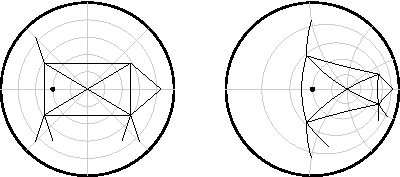
\includegraphics{figures/varphiplot}
\caption{What $\varphi_a$ does to the unit disc.   In this case,
$a=-0.4$ and the position of $a$ and $\varphi_a(a)=0$ is marked with a dot.%
\label{fig:varphiplot}}
\end{myfig}

\begin{prop}
If $f \in \operatorname{Aut}(\D)$, then there exists an $a \in \D$
and $\theta \in \R$ such that
\begin{equation*}
f(z) = e^{i\theta} \frac{z-a}{1-\bar{a}z} = e^{i\theta} \varphi_a(z).
\end{equation*}
\end{prop}

\begin{proof}
Suppose $f(0) = a$.
Consider $g = \varphi_a \circ f$, which is a biholomorphism
and $g(0) = 0$ as
$\varphi_a(a) = 0$.
As in the proof of Schwarz's lemma, we find a holomorphic $h(z)$
such that $g(z) = z h(z)$.  By
Schwarz's lemma, if $z \in \D \setminus \{ 0 \}$, then
\begin{equation*}
\sabs{h(z)} = \frac{\sabs{g(z)}}{\sabs{z}} \leq 1 .
\end{equation*}
Consequently, $h$ is a map of the disc to the closed disc.

But $h$ can have no zeros:
$h(z) = \frac{g(z)}{z}$ cannot be zero for $z \not= 0$ as $g$ is injective
and its one allowed zero is at $z=0$,
and $h(0) = g'(0) \not= 0$.  As $g$ is a biholomorphism, $g^{-1}$ is
continuous. So $g^{-1}(K)$ is compact for any compact $K \subset \D$.
In other words, $\sabs{g(z)}$ must approach $1$ as $z$
approaches the boundary $\partial \D$.
Then so must $\sabs{h(z)}$.
The function
$\sabs{h(z)}$ must, therefore, attain a minimum inside $\D$, or in other
words $\babs{\frac{1}{h(z)}}$ must attain a maximum inside $\D$.  So $h(z)$
is a constant, and $g(z) = \alpha z$ for some constant $\alpha$.
Clearly, 
$\sabs{\alpha} = 1$ or $\alpha = e^{i\theta}$.  Applying
$\varphi_{-a}$ to both sides of $e^{i\theta} z = \varphi_a \circ f$
we obtain
$f(z) = \varphi_{-a}(ze^{i\theta})
= e^{i \theta} \varphi_{-ae^{-i\theta}}(z)$.
\end{proof}

\begin{exbox}
\begin{exercise}
Justify the claim in the proof.  If a continuous
$g \colon \D \to \D$ is is such that $g^{-1}(K)$ is compact
for every compact $K \subset \D$, then if $\{ z_n \}$ is a sequence
in $\D$ such that $\sabs{z_n} \to 1$ then
$\sabs{g(z_n)} \to 1$.
\end{exercise}

\begin{exercise}
Given two distinct $a,b \in \D$, show that there exists a unique 
$f \in \Aut(\D)$
such that $f(a) = b$ and $f(b) = a$.
\end{exercise}

\begin{exercise}
Prove that if $\bH = \{ z \in \C : \Im z > 0 \}$ is the upper half-plane
and $f \colon \bH \to \bH$ is an automorphism of $\bH$, then
\begin{equation*}
f(z) = \frac{a z +b}{c z + d}
\avoidbreak
\end{equation*}
for real numbers $a,b,c,d$ such that $ad-bc \not= 0$.
\end{exercise}

\begin{exercise}
Suppose $U \subset \C$ is open, $\overline{\D} \subset U$,
and $f \colon U \to \C$ is holomorphic.
Suppose $\sabs{f(z)}=1$ whenever $\sabs{z}=1$,
that is, $f(\partial \D) \subset \partial \D$.
Find a formula for $f$.  Use the following outline:
\begin{exparts}
\item
Show that $f$ must have finitely many zeros in $\D$.  That is, $f(z) = 0$
for at most finitely many $z \in \D$.
\item
Suppose that $f$ has no zeros in $\D$.  Prove that $f$ is constant
(and what sort of constant).
\item
If $f(a) = 0$, then prove that
$z \mapsto \frac{f(z)}{\phi_a(z)}$ is still holomorphic in $U$ and
still takes the circle to the circle.
\item
Now find a general formula for $f$.
\end{exparts}
\end{exercise}

\begin{exercise}
Prove the \emph{\myindex{Schwarz--Pick lemma}}:
If $f \colon \D \to \D$ is holomorphic, then
\begin{equation*}
\abs{
\frac{f(z)-f(\zeta)}{1-\overline{f(\zeta)}f(z)}
}
\leq
\abs{
\frac{z-\zeta}{1-\widebar{\zeta}z} 
}
\qquad
\text{and}
\qquad
\frac{\abs{f'(z)}}{1-\abs{f(z)}^2} \leq
\frac{1}{1-\abs{z}^2}
\end{equation*}
for all $z,\zeta \in \D$.
If equality holds in one of the 
inequalities for some $z \not= \zeta$,
then $f$ is an automorphism of $\D$.
Conversely if $f$ is an automorphism of $\D$
then equality holds in both inequalities for
all $z,\zeta \in \D$.
\end{exercise}
\end{exbox}

\pagebreak[0]
In particular, the Schwarz--Pick lemma gives a bound on the derivative
at all points.  If
$f \colon \D \to \D$ is holomorphic, nonconstant, and $f(a) = b$,
then
\begin{equation*}
\sabs{f'(a)} \leq
\frac{1-\sabs{b}^2}{1-\sabs{a}^2} .
\end{equation*}
If equality holds, then $f(z) = \varphi_{-b}\bigl( e^{i\theta} \varphi_a(z)
\bigr)$ for some $\theta \in \R$.

%%%%%%%%%%%%%%%%%%%%%%%%%%%%%%%%%%%%%%%%%%%%%%%%%%%%%%%%%%%%%%%%%%%%%%%%%%%%%%
%%%%%%%%%%%%%%%%%%%%%%%%%%%%%%%%%%%%%%%%%%%%%%%%%%%%%%%%%%%%%%%%%%%%%%%%%%%%%%
%%%%%%%%%%%%%%%%%%%%%%%%%%%%%%%%%%%%%%%%%%%%%%%%%%%%%%%%%%%%%%%%%%%%%%%%%%%%%%

\chapter{The Logarithm and Cauchy} \label{ch:log}

\begin{myquote}
Never doubt the courage of the French. They were the ones who discovered that snails are edible.

---Doug Larson
\end{myquote}

%%%%%%%%%%%%%%%%%%%%%%%%%%%%%%%%%%%%%%%%%%%%%%%%%%%%%%%%%%%%%%%%%%%%%%%%%%%%%%

\section{The logarithm and the winding number}
\label{sec:log}

\subsection{The logarithm}

Let us look at the function $z^n$ for $n \in \Z$.\footnote{It appears,
doesn't it, that elementary complex analysis is the study of $z^n$.}
When $n \geq 0$, 
then $z^n$ is defined in the entire plane, and a primitive is
simply $\frac{z^{n+1}}{n+1}$.  If $n < -1$, then $z^n$ is defined
in the punctured plane $\C \setminus \{0\}$, but again
a primitive is $\frac{z^{n+1}}{n+1}$.  What about $z^{-1} =
\frac{1}{z}$?  It has a primitive, but never defined in
the entire punctured plane.

We proved that in any star-like domain, a holomorphic function has a
primitive.  Consider the so-called \emph{\myindex{slit plane}}
\begin{equation*}
U = \C \setminus (-\infty,0] = \C \setminus \bigl\{ z \in \C : \Re z \leq 0 , \Im z = 0 \bigr\}.
\end{equation*}
It is a star-like domain and
so there exists a
primitive for $\frac{1}{z}$ in $U$.
If we
require that this primitive is $0$ at $z=1$,
we get a function
\glsadd{not:Log}%
\begin{equation*}
\operatorname{Log} \colon U \to \C ,
\end{equation*}
called the \emph{\myindex{principal branch}} of the logarithm.
We had another thing before called the ``principal branch,'' 
the principal branch of the argument.  Let us show that
\begin{equation*}
\Log z = \log \sabs{z} + i \Arg z ,
\end{equation*}
where $\log \sabs{z}$ is just the standard real logarithm.  Let
$L(z) = \log \sabs{z} + i \Arg z$ and let us show that $L = \Log$.  We see
\begin{equation*}
e^{L(z)}
=
e^{\log \sabs{z}} e^{i \Arg z}
=
\sabs{z} e^{i \Arg z} = z .
\end{equation*}
So $L$ is the inverse of the exponential, at least for $z \in U$.
This means in particular that $L$ is holomorphic by the inverse function
theorem.
Take the derivative of both sides of $z = e^{L(z)}$,
\begin{equation*}
1 = L'(z) e^{L(z)} = L'(z) z .
\end{equation*}
Et voil\`a!\footnote{Cauchy was French, n'est pas?}
We have $L'(z) = \frac{1}{z}$, so $L = \Log$.

We could have used any branch of the argument.  We 
make the definition
\glsadd{not:log}%
\begin{equation*}
\log z \overset{\text{def}}{=} \log \sabs{z} + i \arg z .
\end{equation*}
This definition is totally bonkers at first glance.  First, the $\log$ on the
left, is a different $\log$ than the $\log$ on the right.  On the right, it is the
standard real $\log$, that is, $\log \colon (0,\infty) \to \R$,
where $\log 0 = 1$.
But the $\log$ on the left
is now not even a function, it has infinitely many values for every $z$,
since the $\arg$ on the right hand side has infinitely many values.
The value of $\log (-1)$ is $\pi i$, but also $-\pi i$, $3\pi i$,
or $(\pi + 2\pi k)i$ for any $k \in \Z$.  So $\log$ is a function just as much
as $\arg$ is a function.  See \figureref{fig:loggraph}.

\begin{myfig}
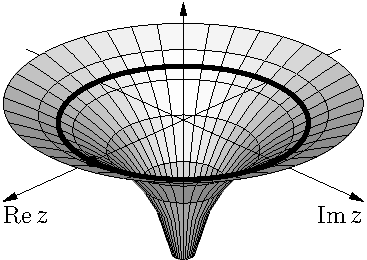
\includegraphics{figures/logrealgraph}
\qquad
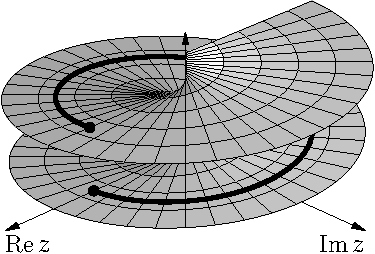
\includegraphics{figures/arggraph2}
\caption{``Graphs'' of the real part (left) and imaginary part (right)
of the complex logarithm $\log z = \log \sabs{z} + i \arg z$.  The imaginary
part is an infinite spiral, only two turns are pictured.  A path on the
graph around the unit circle is marked.\label{fig:loggraph}}
\end{myfig}

The double duty of ``$\log$'' is a small price to pay.  It is almost never a
problem and it is generally clear which $\log$ one is talking about based on
what sort of things are being plugged into it.

While $\log$ is not really a function---it is a multivalued
function\footnote{%
%Countless insufferable smartypants on the internet will try to convince
%you that a ``multivalued function'' isn't a thing.  So better not ask about
%it there.
Cauchy: Quel Malheur!  Je d{\'e}teste le logarithme! Je veux devenir plombier.}---it is really
the definition that we want.
The principal branch, while 
useful when one wants to get some actual numbers, is not always what we
want.  It is not as useful as one would think.
And beware that computers like to give back the principal branch even 
when it doesn't make any sense.

So how do we use $\log$?  Well it comes up in line integrals, which are used
to count and classify zeros and/or singularities of functions, or vice
versa---zeros and singularities are used to compute line integrals.
Let us compute the integral of $\frac{1}{z}$ around the unit
circle $\partial \D$, oriented counterclockwise as usual (parametrized
by $e^{it}$).  Suppose we start and end the integration at 
$z=1$:
\begin{equation*}
\int_{\partial \D} \frac{1}{z} \, dz
= \log 1 - \log 1 = 2\pi i.
\end{equation*}
That makes no sense, no?  Well, it should really only be done
with quotation marks:
\begin{equation*}
\int_{\partial \D} \frac{1}{z} \, dz
\enspace
\text{``$=$''}
\enspace
\log 1 - \log 1
\enspace
\text{``$=$''}
\enspace
2\pi i.
\end{equation*}
That's a lot better,
no?\footnote{Non! Je veux aussi devenir plombier maintenant!}
The equalities are only true morally.
Interpreted correctly, it is exactly what is happening.  You really do subtract
one of the values of $\log 1$ from another value of $\log 1$.  To figure
out which from which, start with say $\log 1 = 0$, and follow the
function along the circle slowly and notice that $i \arg z$ grows from $0$ to
$2\pi i$.  So the $\log 1$ at the end is $2 \pi i$.  See the path
marked on \figureref{fig:loggraph}, the jump in the imaginary part between
the beginning and the end is precisely that $2\pi i$.

To make working with $\log$ easier we usually talk about a
\emph{\myindex{branch of the logarithm}}.  So $L \colon U \to \C$ is a branch
of the logarithm if $L$ is holomorphic, $L'(z) = \frac{1}{z}$, and $L(z)$ is equal
to some value of $\log z$ for every $z \in U$.  It is not possible to define
a branch of the logarithm in every $U$, but for example we can do it in every
star-like $U$ where $0 \notin U$.  In general, one can define a branch of
the logarithm in every simply connected domain, that is, a domain without holes,
that does not contain zero.
More on this later.  Similarly we can define branches of $\log (z-p)$,
a primitive of $\frac{1}{z-p}$, in which case the domain
should not contain $p$.

We may also talk about branches more loosely, and talk
about following them along a path.  That doesn't mean that we really define
a single branch, it means that we define a branch in some small open set,
follow its values for a while, then switch to another branch that 
happens to agree with the first branch at least at the point where we are
at.  See \figureref{fig:followbranch}.  This is really what we did in the
``computation'' above.  We followed $\log$ from $1$ along the circle until we
ended up at $1$ again, and our branches that we followed ended up $2\pi i$
off.  We will see an example of this briefly.

\begin{myfig}
\subimport*{figures/}{followbranch.pdf_t}
\caption{Following a branch.
The branches are defined in the discs
(they do not have to be discs).
Points where the branches are supposed to equal
are marked.\label{fig:followbranch}}
\end{myfig}

\begin{exbox}
\begin{exercise}
Suppose $a \in \C$ is a nonzero complex number, and
$R_a = \{ \lambda a \in \C : \lambda \geq 0 \}$
is the ray from the origin through $a$.  Prove
that there exists a branch of the $\log$ in $\C \setminus R_a$.
\end{exercise}

\begin{exercise}
For $n \in \N$ let $\gamma \colon [0,2\pi] \to \C$ be $\gamma(t) = e^{int}$,
the unit circle traversed $n$ times counterclockwise.  Compute
$\int_\gamma \frac{1}{z} \, dz$.  Try to argue by splitting up the integral
into pieces and using branches of the $\log$.
\end{exercise}

\begin{exercise}
Suppose
$U \subset \C$ is an open set with
$\partial \D \subset U$,
$f \colon U \to \C$ is a holomorphic
function,
such that
$f(z)$ is never negative real or zero.
Compute
$\int_{\partial \D} \frac{f'(z)}{f(z)} \, dz$.
\end{exercise}

\begin{exercise}
Suppose $\gamma \colon [a,b] \to \C \setminus \{ 0 \}$ is a piecewise $C^1$
path such that $\gamma(a) = \gamma(b) = -1$, but $\gamma(t)$ is never
negative real for any $t \in (a,b)$.  Using the principal branch of the
$\log$, prove that
\begin{equation*}
\int_\gamma \frac{1}{z} \, dz = -2\pi i, 0, \text{ or } 2\pi i.
\avoidbreak
\end{equation*}
Find an explicit $\gamma$ that achieves each of these possibilities.
\end{exercise}
\end{exbox}

\subsection{Winding numbers}

OK.  Let's get more rigorous.
%In the following, it is enough
%to consider closed paths, although everything automatically works
%also for cycles (chains that can be written as sums of closed paths,
%or in other words, chains with empty boundary).

\begin{defn}
Let $\Gamma$ be
%a closed piecewise $C^1$ path, or more generally
a cycle,
and $p \notin \Gamma$.  Then
\glsadd{not:windnum}%
\begin{equation*}
n(\Gamma;p)
\overset{\text{def}}{=}
\frac{1}{2\pi i} \int_\Gamma \frac{1}{z-p} \, dz
\end{equation*}
is called the
\emph{\myindex{winding number}} of $\Gamma$ around $p$, or
the 
\emph{\myindex{index}} of $\Gamma$ with respect to $p$.
\end{defn}

Intuitively, the winding number is the number of times that $\Gamma$ winds
around $p$.  This intuition is confirmed by trying to integrate
$\frac{1}{z}$ for the path $e^{it}$ for $t \in [0,2\pi]$, that gets you 
a winding number $1$, as it goes once counterclockwise direction around zero.  If we do
the integral with $e^{2it}$, we go around zero twice in the
counterclockwise direction, and the winding number really is $2$.  Similarly
if we use $e^{-it}$, then we go around zero once in the
clockwise direction, and the winding number is $-1$.

The first thing to prove is to show that the winding number is an integer.

\begin{prop} \label{prop:indexinteger}
Suppose $\Gamma$ is
%a closed piecewise $C^1$ path (or a cycle)
a cycle
and $p \notin \Gamma$.  Then
\begin{equation*}
n(\Gamma;p) = \frac{1}{2\pi i} \int_\Gamma \frac{1}{z-p} \, dz
\avoidbreak
\end{equation*}
is an integer.
\end{prop}

Intuitively, the proof is to take a closed path $\gamma$
and to follow a branch of $\log$ around $\gamma$, and
see by how much it changes.  See \figureref{fig:followbranch}, and we
go all the way around a loop.  Since we really just follow the argument
and we have gone some number of times around $p$ along $\gamma$, the
argument has changed by some multiple of $2\pi$.

\begin{proof}
As a cycle is (equivalent to) a linear combination (over the integers) of closed paths,
then we only need to prove the result for closed piecewise $C^1$ paths.
Let $\gamma \colon [0,1] \to \C$ be the path.
The path $\gamma$ as a set is compact.  It can be covered by finitely many
discs $D_1,\ldots,D_n$, none of which contain $p$, and such that there is a
partition $0 = t_0 < t_1 < t_2 < \cdots < t_n = 1$ such that
$\gamma\bigl([t_{j-1},t_j]\bigr) \subset D_j$.  Each $D_j$ is star-like and
does not contain $p$,
so in each one there exists a branch of $\log (z-p)$, call it $L_j$,
such that $L_j\bigl(\gamma(t_j)\bigr) = L_{j+1}\bigl(\gamma(t_j)\bigr)$
(pick $L_1$ arbitrarily, then pick $L_2,\ldots,L_n$ accordingly).
Call $z_0 = \gamma(0) = \gamma(1)$.  So
\begin{multline*}
n(\gamma;p)
=
\frac{1}{2\pi i} \int_\gamma \frac{1}{z-p} \, dz
=
\frac{1}{2\pi i} \int_0^1 \frac{\gamma'(t)}{\gamma(t)-p} \, dt
=
\frac{1}{2\pi i} \sum_{j=1}^n \int_{t_{j-1}}^{t_j} \frac{\gamma'(t)}{\gamma(t)-p} \, dt
\\
=
\frac{1}{2\pi i} \sum_{j=1}^n L_j\bigl(\gamma(t_j)\bigr) -
L_j\bigl(\gamma(t_{j-1})\bigr)
=
\frac{1}{2\pi i} \bigl( L_n(z_0) - L_1(z_0) \bigr) .
\end{multline*}
As $L_n$ and $L_1$ are both branches of $\log$, their difference is
$2\pi k i$ for some $k \in \Z$, as each is $\log\sabs{z_0} + i \arg z_0$ for some value of
$\arg$.
\end{proof}

\begin{exbox}
\begin{exercise}
Fill in the details in the existence of the partition.  That is, once you
cover $\gamma$ by finitely many discs that do not contain $p$ show that
the partition $t_0,\ldots,t_n$ exists.
\end{exercise}
\end{exbox}

The second thing to notice is that $n(\Gamma;z)$ is constant as long as we
do not cross $\Gamma$.

\begin{prop}
Given
%a piecewise $C^1$ path (or a cycle)
a cycle
$\Gamma$ then
the function $z \mapsto n(\Gamma;z)$ is constant on the
topological components of $\C \setminus \Gamma$.
Furthermore, $n(\Gamma;z) = 0$ for $z$ on the unbounded component
of $\C \setminus \Gamma$.
\end{prop}

As $\Gamma$ is compact, there must be a unique unbounded component
of the complement $\C \setminus \Gamma$, and possibly several bounded
components.
See \figureref{fig:indexconstant} for example.

\begin{myfig}
\subimport*{figures/}{indexconstant.pdf_t}
\caption{Components of $\C \setminus \Gamma$ with the 
winding number around points in those components
marked.\label{fig:indexconstant}}
\end{myfig}

\begin{proof}
Consider the function
\begin{equation*}
p \mapsto n(\Gamma;p) = \frac{1}{2\pi i} \int_\Gamma \frac{1}{z-p} \, dz .
\end{equation*}
Let us show that this function is continuous on $\C \setminus \Gamma$.
Fix $p_0 \in \C \setminus \Gamma$, and let $d = d(p_0,\Gamma)$ be the
distance from 
$p_0$ to $\Gamma$, namely
$d = \inf \bigl\{ \sabs{z-p_0} : z \in \Gamma \bigr\}$.
As $\Gamma$ is compact, $d > 0$.  
For any $p \in \Delta_{d/2}(p_0)$, we have $\sabs{z-p} \geq
\frac{d}{2}$ for every $z \in \Gamma$.  Let $\ell$ be the length of
$\Gamma$, that is $\ell = \int_\Gamma \sabs{dz}$.  Then,
\begin{equation*}
\begin{split}
\abs{n(\Gamma;p_0)-n(\Gamma;p)}
=
\abs{\frac{1}{2\pi i} \int_\Gamma \frac{p_0-p}{(z-p_0)(z-p)} \, dz}
& \leq
\frac{1}{2\pi} \int_\Gamma \frac{\sabs{p_0-p}}{\sabs{z-p_0}\sabs{z-p}} \, \sabs{dz}
\\
& \leq 
\frac{\ell}{\pi {d}^2} \sabs{p_0-p} .
\end{split}
\end{equation*}
So, $n(\Gamma;p)$ is a continuous function of $p$.
As it is continuous
and integer valued, it is constant on any connected component of
$\C \setminus \Gamma$ (the set where it is defined).

Next, for any $p \in \C \setminus \Gamma$,
\begin{equation*}
\sabs{n(\Gamma;p)} \leq \frac{1}{2\pi} \int_\Gamma \frac{1}{\sabs{z-p}} \,
\sabs{dz} \leq \frac{1}{2\pi} \frac{\ell}{d(p,\Gamma)} .
\end{equation*}
On the unbounded component---as $\Gamma$ is compact---we can find $p$
with $d(p,\Gamma)$ arbitrarily large, meaning $n(\Gamma;p)$ is arbitrarily small
on this component, and as it is constant, it must be zero.
\end{proof}

\begin{exbox}
\begin{exercise} \label{exercise:windingcircle}
%FIXME: mark needed/used exercises
%Let $\partial \Delta_r(p)$ be the path oriented counterclockwise.
Show that $n\bigl(\partial \Delta_r(p);z\bigr) = 0$ if $z \notin
\overline{\Delta_r(p)}$ and 
$n\bigl(\partial \Delta_r(p);z\bigr) = 1$ if $z \in \Delta_r(p)$.
\end{exercise}

\begin{exercise}
Let $n \in \Z$ and $\gamma \colon [0,2\pi] \to \C$, where
$\gamma(t) = p + re^{in t}$ be a path, a path that goes $n$ times
counterclockwise around $\partial \Delta_r(p)$.
Prove that
$n\bigl(\gamma;z\bigr) = n$ if $z \in \Delta_r(p)$.
\end{exercise}

\begin{exercise} \label{exercise:windingcircles}
Suppose $0 < r_1 < r_2 < \infty$.
Let $\Gamma = \partial \Delta_{r_2}(p) - \partial \Delta_{r_1} (p)$
(that is, the outside circles goes counterclockwise, the inside circle goes
clockwise).
Prove that if $z \in \C$ is such that $\sabs{z-p} < r_1$ then
$n(\Gamma;z) = 0$.  If $r_1 < \sabs{z-p} < r_2$, then
$n(\Gamma;z) = 1$.  If $r_2 < \sabs{z-p}$, then
$n(\Gamma;z) = 0$.
\end{exercise}

\begin{exercise}
Suppose $\gamma \colon [a,b] \to \C$ be a closed $C^1$ path such that
$\gamma(a) = \gamma(b)$ is some real negative number.  Suppose
that $\gamma(t)$ is real and negative for only $k$ distinct $t$ (and it
includes $a$ and $b$), and whenever $\gamma(t)$ is real and negative,
then $\Im \gamma'(t) < 0$.  Prove that $n(\gamma;0) = k-1$.  Hint: Use
the principal branch.
\end{exercise}
\end{exbox}


%%%%%%%%%%%%%%%%%%%%%%%%%%%%%%%%%%%%%%%%%%%%%%%%%%%%%%%%%%%%%%%%%%%%%%%%%%%%%%

\section{Homology versions of Cauchy}

\begin{defn}
Let $U \subset \C$ be a domain and $\Gamma$
a cycle
%closed piecewise $C^1$ path (or a cycle)
in $U$
such that $n(\Gamma;p) = 0$ for all $p \in \C \setminus U$,
 then we
say $\Gamma$ is \emph{\myindex{homologous to zero} in $U$}.
\end{defn}

What homologous to zero means is that $\Gamma$ does not wind around any
point in the complement of $U$.
Do note that ``homologous to zero'' in no way means ``equivalent to zero.''
For example, if $U = \C$ then every $\Gamma$ is homologous to zero trivially.
Also note the dependence on $U$.  The unit circle is homologous to zero in
$U = \C$, but it is not homologous to zero in $U = \C \setminus \{ 0 \}$.

\begin{thm}[Cauchy integral formula (homology version)]
\index{Cauchy integral formula!homology}
\label{thm:CIFhomology}
Suppose $U \subset \C$ is open, $f \colon U \to \C$ is holomorphic, and
$\Gamma$ is
a cycle
%a closed piecewise $C^1$ path (or a cycle)
in $U$
homologous to zero in $U$.
%such that $n(\Gamma;p) = 0$ for all $p \in \C \setminus U$.
Then for $z \in U \setminus \Gamma$,
\begin{equation*}
n(\Gamma;z)
f(z)
=
\frac{1}{2\pi i}
\int_{\Gamma}
\frac{f(\zeta)}{\zeta-z}
\,
d \zeta .
\end{equation*}
\end{thm}

Before we prove the theorem let us remark
that in the proof, rather strangely, we will define an entire
function (even though $U$ may be small) and then we will use
Liouville's theorem (\thmref{thm:Liouville}).

\begin{proof}
%[Proof of \thmref{thm:CIFhomology}]
%We begin with a expression you have probably seen in the development of the real
%derivative, so it is not a surprise it appears in the development of
%holomorphic functions.
Define $g \colon U \times U \to \C$ by
\begin{equation*}
g(\zeta,z) =
\begin{cases}
\frac{f(\zeta)-f(z)}{\zeta-z} & \text{if } \zeta \not= z , \\
f'(\zeta)                 & \text{if } \zeta = z .
\end{cases}
\end{equation*}

\begin{exbox}
\begin{exercise}
Prove that $g(\zeta,z)$ is continuous in $U \times U$, and that
the function $z \mapsto g(\zeta,z)$ is holomorphic for every fixed $\zeta \in U$.
Hint: The only mildly tricky piece of this proof is showing that $z \mapsto
g(\zeta,z)$ is
holomorphic at $z=\zeta$.
\end{exercise}
\end{exbox}

Let
\begin{equation*}
h(z) = 
\begin{cases}
\int_\Gamma g(\zeta,z) \, d\zeta & \text{if } z \in U , \\
\int_\Gamma \frac{f(\zeta)}{\zeta-z} \, d\zeta & \text{if } z \not \in
\Gamma \text{ and } n(\Gamma;z) = 0 .
\end{cases}
\end{equation*}
As $n(\Gamma;z) = 0$ for all $z \in \C \setminus U$
($\Gamma$ is homologous to zero)
the function $h(z)$ is defined for every $z \in \C$.
Unfortunately, at some points
we have two definitions.
To show that $h(z)$ is well-defined, we must show that if
$n(\Gamma;z) = 0$ and $z \in U$, that we get the same number.
Suppose
we have such a $z$ (in particular $z \notin \Gamma$).  Then,
\begin{equation*}
\int_\Gamma g(\zeta,z) \, d\zeta
=
\int_\Gamma \frac{f(\zeta)-f(z)}{\zeta-z} \, d\zeta
=
\int_\Gamma \frac{f(\zeta)}{\zeta-z} \, d\zeta
-
f(z) n(\Gamma;z)
=
\int_\Gamma \frac{f(\zeta)}{\zeta-z} \, d\zeta .
\end{equation*}
So $h \colon \C \to \C$ is well-defined.

Next we show that $h$ is
holomorphic.
Holomorphicity is a local property, so we only need to prove it 
in a neighborhood of any point.
The set where $n(\Gamma;z) = 0$ is open as it is a
union of topological components of $\C \setminus \Gamma$.
So each point has a neighborhood where $h$ is defined
entirely by one or the other expression above.  Given any point,
take a neighborhood where one of the expressions defines
$h$ and apply \corref{cor:holfuncbyintegral}.

The unbounded component of $\C \setminus \Gamma$ is contained in the
set where $n(\Gamma;z) = 0$, so on this component, $h$ is defined by the
second expression.  Take such a $z$.
Suppose $\sabs{f(\zeta)} \leq M$ for $\zeta \in \Gamma$, let $\ell$ be the length of
$\Gamma$, and let $d(z,\Gamma)$ be the distance of $z$ to $\Gamma$.
\begin{equation*}
\sabs{h(z)}
=
\abs{
\int_\Gamma \frac{f(\zeta)}{\zeta-z} \, d\zeta
}
\leq
\int_\Gamma \abs{\frac{f(\zeta)}{\zeta-z}} \, \sabs{d\zeta}
%\leq
%\int_\Gamma \frac{M}{\sabs{\zeta-z}} \, \sabs{d\zeta}
\leq
\frac{M \ell}{d(z,\Gamma)} .
\end{equation*}
As $z \to \infty$, so does $d(z,\Gamma) \to \infty$, and so $h(z) \to 0$.
In particular, $h$ is an entire bounded function and
Liouville says that $h$ is constant, and that constant must be zero.
So suppose that $z \in U \setminus \Gamma$.  Then
\begin{equation*}
0 = h(z) =
\int_\Gamma \frac{f(\zeta)-f(z)}{\zeta-z} \, d\zeta
=
\int_\Gamma \frac{f(\zeta)}{\zeta-z} \, d\zeta
-
f(z) n(\Gamma;z) . \qedhere
\end{equation*}
\end{proof}

Cauchy's theorem actually follows immediately using the integral formula.

\begin{thm}[Cauchy's theorem (homology version)]
\index{Cauchy's theorem!homology}%
\label{thm:CThomology}%
Suppose $U \subset \C$ is open,
$f \colon U \to \C$ is holomorphic,
and $\Gamma$ is
a cycle
%closed piecewise $C^1$ path (or a cycle)
in $U$
homologous to zero in $U$.
%such that $n(\Gamma;p) = 0$ for
%every $p \in \C \setminus U$,
Then
\begin{equation*}
\int_\Gamma f(z) \, dz = 0 .
\end{equation*}
\end{thm}

\begin{proof}
Fix $z \in U \setminus \Gamma$.  Apply 
the Cauchy integral formula for the function $\zeta \mapsto
(\zeta-z)f(\zeta)$ at $\zeta=z$:
\begin{equation*}
0 = n(\Gamma;z) (z-z)f(z) =
\frac{1}{2\pi i} \int_\Gamma \frac{(\zeta-z)f(\zeta)}{\zeta-z} \, d\zeta
=
\frac{1}{2\pi i} \int_\Gamma f(\zeta) \, d\zeta . \qedhere
\end{equation*}
\end{proof}

\begin{defn}
Two
cycles
%closed piecewise $C^1$ paths (or cycles)
$\Gamma_0$ and $\Gamma_1$ in $U
\subset \C$ are \emph{\myindex{homologous}} in $U$
if $n(\Gamma_0;p) = n(\Gamma_1;p)$ for all $p \in \C \setminus U$.
\end{defn}

Equivalently, $\Gamma_0$ and $\Gamma_1$ are homologous in $U$ if
$n(\Gamma_0 - \Gamma_1;p) = 0$ for all $p \in \C \setminus U$,
that is, $\Gamma_0-\Gamma_1$ is homologous to zero in $U$.

\begin{cor} \label{cor:homologoussameint}
Let $U \subset \C$ be open and $f \colon U \to \C$ holomorphic.
If two
cycles
%closed piecewise $C^1$ paths (or cycles)
$\Gamma_0$ and $\Gamma_1$ in $U$
are homologous in $U$, then
\begin{equation*}
\int_{\Gamma_0} f(z)\, dz = 
\int_{\Gamma_1} f(z)\, dz .
\end{equation*}
\end{cor}

The proof is immediate by applying Cauchy's theorem to $\Gamma_0-\Gamma_1$.

\begin{exbox}
\begin{exercise}
Suppose that $\Gamma$ is
a cycle in $\C \setminus \{ 0 \}$.
Prove that $\Gamma$ is homologous in $\C \setminus \{ 0 \}$
to $n \partial \D$ for some $n \in \Z$.
\end{exercise}

\begin{exercise} \label{exercise:H1U}
\begin{exparts}
\item
Show that being homologous in $U$ is an equivalence relation on cycles.
\item
Prove that the addition of cycles makes the set of equivelence classes
into an abelian group, the
first \emph{\myindex{homology group}}\index{first homology group} of $U$,
usually written $H_1(U)$.
\item
Compute $H_1(\C \setminus \{ 0 \})$ (that is,
find what group is it isomorphic to).
\end{exparts}
\end{exercise}

\begin{exercise}
Suppose that $\Gamma$ is
a cycle
%a closed piecewise $C^1$ path (or cycle)
such that
$n(\Gamma;0) = k$.  Compute
\begin{equation*}
\int_{\Gamma} \frac{1}{z} \, dz .
\end{equation*}
\end{exercise}

\begin{exercise}
Prove that the two theorems
(the homology versions of Cauchy's theorem and the Cauchy integral formula)
are equivalent logically, that is, one follows
from the other.  We have already proved that the Cauchy integral formula
implies Cauchy's theorem.  So prove that
Cauchy's theorem implies the Cauchy integral formula.
\end{exercise}

\begin{exercise}
Suppose $U \subset \C$ is open and $\Gamma$ 
is
%a closed piecewise $C^1$ path (or cycle)
a cycle
in $U$
homologous to zero in $U$.
%such that
%$n(\Gamma;p) = 0$ for all $p \in \C \setminus U$.
Suppose that $n(\Gamma;z_1) = k_1$ and  $n(\Gamma;z_2) = k_2$ for
some two distinct $z_1,z_2 \in U \setminus \Gamma$.
Suppose $f \colon U \setminus \{z_1,z_2\} \to \C$ is
holomorphic.
Suppose $0< \epsilon < \sabs{z_1-z_2}$ is small enough that
$\overline{\Delta_\epsilon(z_j)} \subset U$ for $j=1,2$,
and suppose that
$\int_{\partial \Delta_\epsilon(z_1)} f(z) \, dz = A$ and 
$\int_{\partial \Delta_\epsilon(z_2)} f(z) \, dz = B$.
Compute
\begin{equation*}
\int_{\Gamma} f(z) \, dz
\end{equation*}
in terms of $k_1$, $k_2$, $A$, and $B$.
\end{exercise}
\end{exbox}


%%%%%%%%%%%%%%%%%%%%%%%%%%%%%%%%%%%%%%%%%%%%%%%%%%%%%%%%%%%%%%%%%%%%%%%%%%%%%%

\section{Simply connected domains}

A simply connected domain\footnote{%
There is no agreement among various mathematicians (I've asked a few) if
a disconnected set can be ``simply connected.''
To avoid heated arguments with topologists of various stripes,
it's best to just not define the term for (path-)disconnected sets.
Hence, we only define it for domains.}
is one without any holes.  The following is
perhaps not the standard definition, but for domains of $\C$
(connected open sets)
it is sufficient.  We will define the term ``properly'' once we get 
to homotopy.  We may sometimes say ``simply connected in the sense of
homology'' to emphasize that we are using this definition, but in this book,
a ``simply connected domain'' is this particular definition.

\begin{defn} \label{defn:simplyconnected:homology}
A domain $U \subset \C$ is \emph{\myindex{simply connected}}
if every cycle in $U$
is homologous to zero in $U$.
\end{defn}

In other words, $U$ is simply connected
if for every cycle $\Gamma$, we have $n(\Gamma;p) = 0$
every $p \in \C \setminus U$.
So in a simply connected domain, no cycle in $U$ can wind around any piece of $\C \setminus U$.


\begin{exbox}
\begin{exercise}
Prove that $\C$ and $\D$ are simply connected, and $\C \setminus \{ 0 \}$
is not simply connected.
\end{exercise}

\begin{exercise}
Prove that $U \subset \C$ is simply connected if and only if
the first homology group
$H_1(U)$ is isomorphic to the trivial group $\{ 0 \}$.
See \exerciseref{exercise:H1U}.
\end{exercise}

\begin{exercise}
Prove that any star-like domain in $\C$ is simply connected.
\end{exercise}
\end{exbox}

A special (but common) case of the homology version of Cauchy,
\thmref{thm:CThomology}, can be stated as the simply connected case of Cauchy.

\begin{thm}[Cauchy's theorem (simply connected version)]
\index{Cauchy's theorem!simply connected}%
Let $U \subset \C$ be a simply connected domain and $f \colon U \to \C$
holomorphic.  If $\Gamma$ is
a cycle
%a closed piecewise $C^1$ path (or a cycle)
in $U$, then
\begin{equation*}
\int_\Gamma f(z) \, dz = 0 .
\end{equation*}
\end{thm}

The proof follows at once from \thmref{thm:CThomology},
since if $U$ is simply connected, then
every $\Gamma$ in $U$ is homologous to zero in $U$.
%$n(\Gamma;p) = 0$ for every cycle $\Gamma$ in $U$.
Having Cauchy's theorem in simply connected
domains for all cycles,
we have primitives (antiderivatives) in simply connected
domains.

\begin{thm}
Let $U \subset \C$ be a simply connected domain and
let $f \colon U \to \C$ be holomorphic.  Then $f$ has a
primitive in $U$.
\end{thm}

\begin{proof}
Fix some $p \in U$. As $U$ is path connected, for every $z \in U$, pick
some piecewise $C^1$ path $\gamma$ from $p$ to $z$
and define
\begin{equation*}
F(z) = \int_\gamma f(\zeta) \, d\zeta .
\end{equation*}
A priory, the function $F(z)$ depends on $\gamma$, but Cauchy's
theorem says that if $\alpha$ is another path from $p$ to $z$, then
\begin{equation*}
\int_\gamma f(\zeta) \, d\zeta -
\int_\alpha f(\zeta) \, d\zeta 
=
\int_{\gamma-\alpha} f(\zeta) \, d\zeta  =  0 .
\end{equation*}
So $F$ is well-defined without specifying the path.

The rest of the proof can be done analogously to the proof for star-like
domains (\propref{prop:primitiveinstarlike1} and
\corref{cor:primitiveinstarlike}) .  Let us just reduce it to that case.
Let $q \in U$ be a point and consider a disc $\Delta_r(q) \subset U$
(which is star-like with respect to $q$ in particular).
We take $\gamma$ to be the path from $p$ to $q$.
As $F$ does not depend on the path taken, then for $z \in \Delta_r(q)$,
\begin{equation*}
F(z) =
\int_{\gamma+[q,\zeta]} f(\zeta) \, d\zeta
=
\int_{\gamma} f(\zeta) \, d\zeta
+
\int_{[q,\zeta]} f(\zeta) \, d\zeta .
\end{equation*}
The first term in the sum is a constant, and the second term is precisely
the primitive of $f$ for star-like domains, that is, the primitive in
$\Delta_r(q)$.
See \figureref{fig:anyantidef}.
\end{proof}

\begin{myfig}
\subimport*{figures/}{anyantidef.pdf_t}
\caption{Existence of primitive in a simply connected
domain with the disc $\Delta_r(q)$ marked.\label{fig:anyantidef}}
\end{myfig}

\begin{cor}
Let $U \subset \C$ be a simply connected domain and
let $f \colon U \to \C$ be a nowhere zero holomorphic
function.  Then there exists a holomorphic $g \colon U \to \C$
such that
\begin{equation*}
e^{g(z)} = f(z) .
\end{equation*}
\end{cor}

In particular, using $f(z) = z$ we find that if
$U \subset \C \setminus \{ 0 \}$ is a simply connected domain, then
there exists a branch of the logarithm, that is,
a holomorphic $L \colon U \to \C$ such that
\begin{equation*}
e^{L(z)} = z .
\end{equation*}

\begin{proof}
The function $\frac{f'(z)}{f(z)}$ is holomorphic on $U$.
Find a primitive $g(z)$.  Compute
\begin{equation*}
\frac{d}{dz} \left[ \frac{e^{g(z)}}{f(z)} \right] =
\frac{ e^{g(z)} g'(z) f(z) - e^{g(z)} f'(z) }{{\bigl(f(z)\bigr)}^2}
=
\frac{ e^{g(z)} f'(z) - e^{g(z)} f'(z) }{{\bigl(f(z)\bigr)}^2}
=
0 .
\end{equation*}
Thus, $\frac{e^{g(z)}}{f(z)}$ is constant
(\propref{prop:zeroder}).  It follows that
there is a $C \in \C$ such that
\begin{equation*}
e^{g(z) + C} = f(z) .
\qedhere
\end{equation*}
\end{proof}

If we have the logarithm, we can take roots.

\begin{cor}
Let $U \subset \C$ be a simply connected domain,
let $f \colon U \to \C$ be a nowhere zero holomorphic
function, and let $k \in \N$.
Then there exists a holomorphic $g \colon U \to \C$
such that
\begin{equation*}
{\bigl(g(z)\bigr)}^k = f(z) .
\end{equation*}
\end{cor}

\begin{proof}
Find a $\psi \colon U \to \C$ such that $e^{\psi(z)} = f(z)$.  Let
$g(z) = e^{\frac{1}{k} \psi(z)}$.  Check:
\begin{equation*}
{\bigl(g(z)\bigr)}^k
=
{\left( e^{\frac{1}{k} \psi(z)} \right)}^k
e^{\psi(z)} = f(z) . \qedhere
\end{equation*}
\end{proof}

On the other hand, the existence of primitives or
Cauchy's theorem without restriction on $\Gamma$ guarantees
simply-connectedness.  In particular, we have the following set of equivalent
versions of simply-connectedness for domains.

\begin{prop}
Let $U \subset \C$ be a domain.  The following are equivalent:
\begin{enumerate}[(i)]
\item \label{thm:simplyconnected:i}
$U$ is simply connected (in the homology sense).
\item \label{thm:simplyconnected:ii}
Every holomorphic $f \colon U \to \C$ has a primitive.
\item \label{thm:simplyconnected:iii}
$\frac{1}{z-p}$ has a primitive in $U$ for every $p \in \C \setminus U$.
\item \label{thm:simplyconnected:iv}
For every holomorphic $f \colon U \to \C$ and every
cycle
%closed piecewise $C^1$ path (or a cycle)
$\Gamma$ in $U$, we have
\begin{equation*}
\int_\Gamma f(z) \, dz = 0 .
\end{equation*}
\item \label{thm:simplyconnected:v}
For every $p \in \C \setminus U$ and every
cycle
%closed piecewise $C^1$ path (or a cycle)
$\Gamma$ in $U$, we have
\begin{equation*}
\int_\Gamma \frac{1}{z-p} \, dz = 0 .
\end{equation*}
\end{enumerate}
\end{prop}

\begin{proof}
The logic of the proof is the following diagram:
\begin{equation*}
\begin{tikzcd}[cramped, row sep=small]
& \text{\ref{thm:simplyconnected:ii}} \arrow[d, Rightarrow] \arrow[dr, Rightarrow] & \\
\text{\ref{thm:simplyconnected:i}} \arrow[ur, Rightarrow] & 
\text{\ref{thm:simplyconnected:iv}} \arrow[d, Rightarrow] &
\text{\ref{thm:simplyconnected:iii}} \arrow[dl, Rightarrow] \\
& \text{\ref{thm:simplyconnected:v}} \arrow[ul, Leftrightarrow] &
\end{tikzcd}
\end{equation*}
We proved
\ref{thm:simplyconnected:i} $\Rightarrow$
\ref{thm:simplyconnected:ii} above,
and
\ref{thm:simplyconnected:ii} $\Rightarrow$
\ref{thm:simplyconnected:iii} is immediate.
Using Cauchy's theorem for derivatives (\corref{cor:cauchyforders}),
\ref{thm:simplyconnected:iii} implies
\begin{equation*}
\int_\Gamma \frac{1}{z-p} \, dz = 0 
\end{equation*}
for every $p \in \C \setminus U$,
and hence 
\ref{thm:simplyconnected:v} is true.
As 
\begin{equation*}
n(\Gamma;p) = 
\frac{1}{2\pi i}
\int_\Gamma \frac{1}{z-p} \, dz ,
\end{equation*}
\ref{thm:simplyconnected:v} is simply a restatement of
\ref{thm:simplyconnected:i}.
Again by Cauchy's theorem for derivatives,
\ref{thm:simplyconnected:ii} $\Rightarrow$
\ref{thm:simplyconnected:iv}.
And finally, \ref{thm:simplyconnected:iv} $\Rightarrow$
\ref{thm:simplyconnected:v} is immediate.
\end{proof}

There is a simple topological criterion for
simply-connectedness of domains in the complex plane.
The theorem is actually an ``if and only if,'' but the other
direction is more difficult and so let's just prove the easy direction
at this point.
The other direction will be much easier to prove once we have the Riemann
mapping theorem, see \subsectionref{subsec:patharoundK}, so we will
prove it there.

\begin{prop} \label{prop:scbycomplementeasy}
Let $U \subset \C$ be a domain.  If
$\C_\infty \setminus U$ is connected, then $U$ is simply connected.
\end{prop}

\begin{proof}
Take $S = \C_\infty \setminus U$ and let $\Gamma$ be a cycle in $U$.
The function $\varphi(z)= n(\Gamma;z)$ is continuous on 
$\C \setminus \Gamma$,
therefore $\varphi$ is a continuous function on $S \setminus \{
\infty \}$.  On the unbounded component of $\C \setminus \Gamma$ the
function is zero, and so $\varphi$ is zero in a neighborhood of $\infty$ and so
if we set $\varphi(\infty) = 0$, the function is continuous
on $\C_\infty \setminus \Gamma$.  As $S$ is connected
it is contained in
a single component of $\C_\infty \setminus \Gamma$ so $\varphi$ is
constant on $S$.  As $\varphi(\infty) = 0$, $\varphi|_S \equiv 0$.  In
other words, $U$ is simply connected.
\end{proof}

It is important to use $\C_\infty$ and not $\C$ in the proposition
above.  If $U = \C \setminus \{ 0 \}$ is the punctured plane then
$\C \setminus U = \{ 0 \}$ which is connected, but 
$\C_\infty \setminus U = \{ 0, \infty \}$ is not connected.

\begin{exbox}
\begin{exercise}
Suppose $U \subset \C$ is a domain, $\partial \Delta_r(p) \subset U$,
but there is a $z \in \Delta_r(p)$ such that $z \notin U$.
Prove that $U$ is not simply connected.
\end{exercise}

\begin{exercise}
Let $K \subset \C$ be nonempty and compact.
Prove that the unbounded component of $\C \setminus K$ is not a
simply connected domain.
\end{exercise}

\begin{exercise}
Let $U_1,U_2 \subset \C$ be two simply connected domains such that $U_1 \cap
U_2$ is nonempty and connected.
Prove that $U = U_1 \cup U_2$ is a simply connected domain.
\end{exercise}

\begin{exercise}
Let $U_1,U_2 \subset \C$ be two simply connected domains such that $U_1 \cap
U_2$ is nonempty and connected.
Prove that $U = U_1 \cap U_2$ is a simply connected domain.
Note: This is true in the plane but it is no longer true in the Riemann
sphere, or any more general topological space.
\end{exercise}

\begin{exercise}
Find two nonempty simply connected domains
$U_1,U_2 \subset \C$ such that $U_1 \cap U_2$ is nonempty and both
\begin{exnumparts}
\item
$U_1 \cup U_2$ is not a simply connected domain.
\item
$U_1 \cap U_2$ is not a simply connected domain (emphasis on domain).
\end{exnumparts}
\end{exercise}

\begin{exercise}
Suppose $U \subset \C$ is a simply connected domain such that $0 \notin U$,
there exist some positive real numbers in $U$, and that $r \in \R$.
Show that there exists a holomorphic $f \colon U \to \C$ such
that $f(x) = x^r$ for all $x > 0$ in $U$.
\end{exercise}

\begin{exercise}
Find a simply connected domain $U \subset \C$ such that $\C \setminus U$
has infinitely many components ($\C_\infty \setminus U$ is still going to
have just one component).
\end{exercise}
\end{exbox}

%%%%%%%%%%%%%%%%%%%%%%%%%%%%%%%%%%%%%%%%%%%%%%%%%%%%%%%%%%%%%%%%%%%%%%%%%%%%%%

\section{Laurent series}

One can also define a series for a holomorphic function around a hole, or a singularity.

\begin{defn}
Given $0 \leq r_1 < r_2 \leq \infty$ and $p \in \C$, define
\glsadd{not:annulus}%
\begin{equation*}
\ann(p;r_1,r_2)
\overset{\text{def}}{=}
\{ z \in \C : r_1 < \sabs{z - p} < r_2 \} .
\end{equation*}
When $0 < r_1 < r_2 < \infty$ we call this set an
\emph{\myindex{annulus}}\footnote{%
Q: What do you call a banana with a hole?
A: A banannulus.}.
\end{defn}

A common case we see often is when $r_1 = 0$, that is,
the punctured disc
\begin{equation*}
\ann(p;0,r) = \Delta_r(p) \setminus \{ p \} .
\end{equation*}
When $r_2 = \infty$ on the other hand,
$\ann(p;r,\infty) = \C \setminus \overline{\Delta_{r}(p)}$ (if $r > 0$).  We will,
however, avoid temptation calling $\ann(p;r,\infty)$ an ``annulus.''%
\footnote{``Holey plane'' perhaps?  A punctured disc also ought not to be
called an ``annulus'', and calling $\ann(0;0,\infty) = \C \setminus
\{ 0 \}$ an ``annulus'' is right out!}

\begin{thm}[\myindex{Existence of Laurent series}]
\index{Laurent series!existence}%
\label{thm:laurent}%
Suppose that $0 \leq r_1 < r_2 \leq \infty$ and
$f \colon \ann(p;r_1,r_2) \to \C$ is holomorphic.
Then there exist unique numbers $c_n \in \C$ for $n \in \Z$ such that
\begin{equation*}
f(z) = \sum_{n=-\infty}^{\infty} c_n {(z-p)}^n ,
\end{equation*}
where the convergence is uniformly absolute on every compact subset of
$\ann(p;r_1,r_2)$.  The numbers $c_n$ are given by
\begin{equation*}
c_n = 
\frac{1}{2\pi i}
\int_{\gamma}
\frac{f(z)}{{(z-p)}^{n+1}}
\,
dz  ,
\end{equation*}
where $\gamma$ is any circle of radius $s$, $r_1 < s < r_2$, centered at
$p$ oriented counterclockwise.
\end{thm}

Recall that convergence of a double series such as
\begin{equation*}
\sum_{n=-\infty}^{\infty} a_n
\end{equation*}
means
\begin{equation*}
\sum_{n=-\infty}^{\infty} a_n
=
\lim_{N\to -\infty}
\sum_{n=N}^{-1} a_n
+
\lim_{M\to \infty}
\sum_{n=0}^{M} a_n .
\end{equation*}
That is, the limits are taken independently.  However, for the series we
are interested in, we are generally talking
about absolute convergence, so the limit may be taken in any way, and in any order.
When working with Laurent series in particular we know even more.
Write a Laurent series as 
\begin{multline*}
\sum_{n=-\infty}^{\infty} c_n {(z-p)}^n
=
\sum_{n=0}^{\infty} c_n {(z-p)}^n
+
\sum_{n=-\infty}^{-1} c_n {(z-p)}^n
\\
=
\sum_{n=0}^{\infty} c_n {(z-p)}^n
+
\sum_{n=1}^{\infty} c_{-n} {\left(\frac{1}{z-p}\right)}^n .
\end{multline*}
So the Laurent series behaves like two power series: one in $z-p$ and one
in $\frac{1}{z-p}$.  You can therefore apply what you know about power
series.

\begin{proof}[Proof of the theorem]
Choose two numbers $s_1$ and $s_2$ such that $r_1 < s_1 < s_2 < r_2$.
Define the cycle
\begin{equation*}
\Gamma = \partial \Delta_{s_2}(p) - \partial \Delta_{s_1}(p) .
\end{equation*}
That is, $\Gamma$ goes around the larger ($s_2$) circle counterclockwise and
around the smaller ($s_1$) circle clockwise.

If $q \in \C \setminus \ann(p;r_1,r_2)$, then $n(\Gamma;q) = 0$:
If $q$ is in the ``hole'' of the annulus, then
$n\bigl(\partial \Delta_{s_j}(p);q\bigr) = 1$ for both $j=1,2$, and 
if $q$ is outside the annulus altogether then
$n\bigl(\partial \Delta_{s_j}(p);q\bigr) = -1$ for both $j=1,2$,
see \exerciseref{exercise:windingcircle} or.
\exerciseref{exercise:windingcircles}.
So $\Gamma$ is homologous to zero in the annulus.
On the other hand if $q$ is in the (smaller) annulus $\ann(p;s_1,s_2)$,
then for similar reasons, $n(\Gamma;q) = 1$.

Via Cauchy's theorem (\thmref{thm:CThomology}), for every $z \in \ann(p;s_1,s_2)$,
\begin{equation*}
f(z) = 
\frac{1}{2\pi i}
\int_{\Gamma} \frac{f(\zeta)}{\zeta-z} \, d\zeta 
=
\frac{1}{2\pi i}
\int_{\partial \Delta_{s_2}(p)} \frac{f(\zeta)}{\zeta-z} \, d\zeta 
-
\frac{1}{2\pi i}
\int_{\partial \Delta_{s_1}(p)} \frac{f(\zeta)}{\zeta-z} \, d\zeta  .
\end{equation*}
See \figureref{fig:twoannuli}.


\begin{myfig}
\subimport*{figures/}{twoannuli.pdf_t}
\caption{The two annuli, the smaller annulus is shaded darker.  The two
pieces of $\Gamma$ are noted with the circular arrows.\label{fig:twoannuli}}
\end{myfig}


Let us expand the two bits separately.  First
if $\zeta \in \partial \Delta_{s_2}$, then
$\babs{\frac{z-p}{\zeta-p}} = \frac{\sabs{z-p}}{s_2} < 1$ and so
we follow the logic of \thmref{thm:holpower}.  The reason that we can
swap the integral and the series limit is the same as in that theorem.
\begin{equation*}
\begin{split}
\frac{1}{2\pi i}
\int_{\partial \Delta_{s_2}(p)} \frac{f(\zeta)}{\zeta-z} \, d\zeta 
& =
\frac{1}{2\pi i}
\int_{\partial \Delta_{s_2}(p)} \frac{f(\zeta)}{\zeta-p}
\frac{1}{1-\frac{z-p}{\zeta-p}} \, d\zeta
\\
& =
\frac{1}{2\pi i}
\int_{\partial \Delta_{s_2}(p)} \frac{f(\zeta)}{\zeta-p}
\sum_{n=0}^\infty
{\left(\frac{z-p}{\zeta-p}\right)}^n \, d\zeta
\\
& =
\sum_{n=0}^\infty
\underbrace{
\left(
\frac{1}{2\pi i}
\int_{\partial \Delta_{s_2}(p)} \frac{f(\zeta)}{{(\zeta-p)}^{n+1}}
 \, d\zeta
\right)
}_{c_n}
{(z-p)}^n .
\end{split}
\end{equation*}

Similarly, 
if $\zeta \in \partial \Delta_{s_1}$, then
$\babs{\frac{\zeta-p}{z-p}} = \frac{s_1}{\sabs{z-p}} < 1$ and so
\begin{equation*}
\begin{split}
-\frac{1}{2\pi i}
\int_{\partial \Delta_{s_1}(p)} \frac{f(\zeta)}{\zeta-z} \, d\zeta 
& = 
\frac{1}{2\pi i}
\int_{\partial \Delta_{s_1}(p)} \frac{f(\zeta)}{z-p}
\frac{1}{1-\frac{\zeta-p}{z-p}} \, d\zeta
\\
& =
\frac{1}{2\pi i}
\int_{\partial \Delta_{s_1}(p)} \frac{f(\zeta)}{z-p}
\sum_{m=0}^\infty
{\left(\frac{\zeta-p}{z-p}\right)}^m \, d\zeta
\\
& =
\sum_{m=0}^\infty
\left(
\frac{1}{2\pi i}
\int_{\partial \Delta_{s_1}(p)} f(\zeta){(\zeta-p)}^{m}
 \, d\zeta
\right)
{(z-p)}^{-m-1} .
\\
& =
\sum_{n=-\infty}^{-1}
\underbrace{
\left(
\frac{1}{2\pi i}
\int_{\partial \Delta_{s_1}(p)} \frac{f(\zeta)}{{(\zeta-p)}^{n+1}}
 \, d\zeta
\right)
}_{c_n}
{(z-p)}^{n} .
\end{split}
\end{equation*}
Adding these together we have the right thing, except the formula for $c_n$
is not quite right.  Given any $s$ such that
$r_1 < s < r_2$,
the cycle
$\partial \Delta_{s}(p) - \partial \Delta_{s_1}(p)$ is homologous to zero in
$\ann(p;r_1,r_2)$, and 
$z \mapsto \frac{f(z)}{{(z-p)}^{n+1}}$ is holomorphic in 
$\ann(p;r_1,r_2)$.  Cauchy's theorem (\thmref{thm:CThomology}) thus says
\begin{equation*}
0 = \int_{\partial \Delta_{s}(p) - \partial \Delta_{s_1}(p)}
\frac{f(\zeta)}{{(\zeta-p)}^{n+1}} \, d\zeta
=
\int_{\partial \Delta_{s}(p)}
\frac{f(\zeta)}{{(\zeta-p)}^{n+1}} \, d\zeta
-
\int_{\partial \Delta_{s_1}(p)}
\frac{f(\zeta)}{{(\zeta-p)}^{n+1}} \, d\zeta .
\end{equation*}
Similarly for $s_2$, and hence
\begin{equation*}
c_n = \frac{1}{2\pi i}
\int_{\partial \Delta_{s}(p)} \frac{f(\zeta)}{{(\zeta-p)}^{n+1}}
 \, d\zeta .
\end{equation*}
So we get the same $c_n$ no matter which $s$ we pick.

Next, convergence.
For any $\epsilon > 0$,
the geometric series used for the first part converges uniformly
absolutely when $\babs{\frac{z-p}{\zeta-p}} = \frac{\sabs{z-p}}{s_2} \leq
1-\epsilon$.  In other words, the series converges uniformly absolutely
on compact subsets of $\Delta_{s_2}(p)$ (when $\sabs{z-p} < s_2$).
%
The geometric series used for the second part converges uniformly
absolutely when $\babs{\frac{\zeta-p}{z-p}} = \frac{s_1}{\sabs{z-p}} \leq
1-\epsilon$.  In other words, the series converges uniformly absolutely
on compact subsets of $\C \setminus \Delta_{s_1}(p)$ (when $\sabs{z-p} > s_1$).
%
Hence both parts (and so the entire series) 
converge uniformly absolutely on compact
subsets of $\ann(p;s_1,s_2)$.  As $s_1$ and $s_2$ were arbitrary such that
$r_1 < s_1 < s_2 < r_2$, we get that the series
converges uniformly absolutely on compact subsets of $\ann(p;r_1,r_2)$.

Finally, uniqueness of $c_n$.  Suppose $\{ d_n \}$ is another sequence such
that
\begin{equation*}
f(z)
=
\sum_{n=-\infty}^{\infty} d_n {(z-p)}^{n} 
\end{equation*}
with uniform absolute convergence on compact subsets of $\ann(p;r_1,r_2)$.
Then
\begin{equation*}
\begin{split}
c_m = \frac{1}{2\pi i}
\int_{\partial \Delta_{s}(p)} \frac{f(\zeta)}{{(\zeta-p)}^{m+1}}
 \, d\zeta 
& =
\frac{1}{2\pi i}
\int_{\partial \Delta_{s}(p)}
\left(\sum_{n=-\infty}^{\infty} d_n {(\zeta-p)}^{n} \right)
\frac{1}{{(\zeta-p)}^{m+1}}
 \, d\zeta 
\\
& =
\frac{1}{2\pi i}
\sum_{n=-\infty}^{\infty}
d_n
\int_{\partial \Delta_{s}(p)}
{(\zeta-p)}^{n-m-1}
 \, d\zeta 
\\
& =
d_m ,
\end{split}
\end{equation*}
as the only $n$ for which
$\int_{\partial \Delta_{s}(p)}
{(\zeta-p)}^{n-m-1}
 \, d\zeta$ is nonzero is when $n=m$, that is when we are integrating
${(\zeta-p)}^{-1}$, in which case we get $2 \pi i$.
\end{proof}

Similarly to the power series, due to the uniqueness of the Laurent series,
it does not matter how we obtain it.  For example, the function $e^{1/z}$
has the Laurent series
\begin{equation*}
e^{1/z}
=
\sum_{n=0}^{\infty} \frac{1}{n!} {\left(\frac{1}{z}\right)}^n
=
\sum_{n=-\infty}^0 \frac{1}{(-n)!} z^n ,
\end{equation*}
which converges uniformly absolutely on compact subsets of
$\C \setminus \{ 0 \}$.

The rational function $\frac{1}{1-z}$ that leads to the geometric series can
be expanded in a slightly different way if we want its Laurent series
expansion in $\ann(0;1,\infty) = \C \setminus \overline{\D}$:
\begin{equation*}
\frac{1}{1-z}
=
\frac{-1}{z}
\frac{1}{1-\frac{1}{z}}
=
\frac{-1}{z}
\sum_{n=0}^\infty
{\left(\frac{1}{z}\right)}^n
=
\sum_{n=-\infty}^{-1}
- z^{n} ,
\end{equation*}
which converges in $\ann(0;1,\infty)$.

Finally, while in general a Laurent series is not a power series,
it could very well be when all the $c_n$ for negative $n$ are zero.

\begin{exbox}
\begin{exercise}[Easy]
Suppose $f \colon \Delta_r(p) \to \C$ is holomorphic, and suppose you expand
$f$ in a Laurent series in $\ann(p;r_1,r_2)$ for $0 \leq r_1 < r_2 \leq r$.
Prove that $c_n = 0$ for all negative $n$ and that $c_n$ for nonnegative $n$
are the coefficients of the power series of $f$ at $p$.
\end{exercise}

\begin{exercise}[Easy]
Suppose $f$ and $g$ are holomorphic functions defined on
$\ann(p;r_1,r_2)$.  Let $a_n$ be the coefficients in the Laurent series for
$f$ and $b_n$ be the coefficients in the Laurent series for $g$.  Suppose
that $\alpha,\beta \in \C$.  Show that the Laurent series for the function
$\alpha f + \beta g$ has coefficients $\alpha a_n + \beta b_n$.
\end{exercise}

\begin{exercise}[Easy]
Suppose $\sum_{n=-\infty}^m c_n {(z-p)}^n$ is a Laurent series with only
finitely many positive terms.  Show that either the series converges
nowhere, or there exists a number $r \geq 0$ such that the series
converges uniformly and absolutely on compact subsets of
$\ann(p;r,\infty)$.
\end{exercise}

\begin{exercise}
Expand the function $\frac{1}{(z-1)(z-2)}$ using Laurent (or power) series in 
\begin{exparts}
\item $\ann(0;0,1) = \D \setminus \{ 0 \}$,
\item $\ann(0;1,2)$,
\item $\ann(0;2,\infty)$.
\end{exparts}
\end{exercise}

\begin{exercise}
Suppose $U = \ann(p;r_1,r_2)$ and $r_1 < r < r_2$.
Show that every cycle $\Gamma$ in $U$ is homologous in $U$
to $n \partial \Delta_r(p)$ for some integer $n$.
\end{exercise}

\begin{exercise}
Suppose $f \colon \ann(p;r_1,r_2) \to \C$ is holomorphic,
$r_1 < s < r_2$, and
\begin{equation*}
\int_{\partial \Delta_{s}(p)} f(z){(z-p)}^n
 \, dz = 0
\end{equation*}
for all nonnegative integers $n$.  Prove that $f$ extends through the hole:
There exists a holomorphic $g \colon \Delta_{r_2}(p) \to \C$ such that 
$f = g$ on $\ann(p;r_1,r_2)$.
\end{exercise}

\begin{exercise}
Suppose $f$ is a holomorphic function defined in a domain that contains
the unit circle $\partial \D$, such that
\begin{equation*}
\int_{\partial \D} f(z)\bar{z}^n
 \, dz = 0
\end{equation*}
for all integers $n \in \Z$.  Prove that $f \equiv 0$.
\end{exercise}

\begin{exercise}
Show that for a Laurent series it is again enough to show convergence
somewhere.  Suppose $\sum_{n=-\infty}^\infty c_n {(z-p)}^n$ is a Laurent
series that converges at $z_1$ and $z_2$ where
$0 < \sabs{z_1} < \sabs{z_2} < \infty$.
Prove that the series converges uniformly absolutely on compact subsets
of $\ann(p;\sabs{z_1},\sabs{z_2})$.
\end{exercise}
\end{exbox}

%%%%%%%%%%%%%%%%%%%%%%%%%%%%%%%%%%%%%%%%%%%%%%%%%%%%%%%%%%%%%%%%%%%%%%%%%%%%%%

\section{Homotopy version of Cauchy *}

\subsection{Homotopy}

We wish to make precise the notion of slowly deforming one path into
another.  This notion is usually called \emph{\myindex{homotopy}}.
First, let us define this concept for closed paths.

\begin{defn}
Let $U \subset \C$ be open.
Two closed piecewise $C^1$ paths\footnote{This definition
works for any continuous functions $\gamma_0$ and $\gamma_1$ such that
$\gamma_j(a)=\gamma_j(b)$, but we only need it for paths.}
$\gamma_0 \colon [a,b] \to U$ and
$\gamma_1 \colon [a,b] \to U$ are \emph{\myindex{homotopic}} in $U$
(or relative to $U$) if there exists a continuous function
$H \colon [a,b] \times [0,1] \to U$ such that
for all $s$ and $t$
\begin{equation*}
H(t,0) = \gamma_0(t), \qquad
H(t,1) = \gamma_1(t), \qquad \text{and} \qquad
H(a,s) = H(b,s) .
\end{equation*}
\end{defn}

\begin{exbox}
\begin{exercise}
Show that homotopy is an equivalence relation on continuous functions
$\gamma \colon [a,b] \to \C$ with $\gamma(a)=\gamma(b)$.
\end{exercise}
\end{exbox}

\begin{example} \label{example:homotopydiscsc}
Let $\gamma \colon [a,b] \to \D$ be a continuous function.  Define
$H \colon [a,b] \times [0,1] \to \D$ by
\begin{equation*}
H(t,s) = (1-s) \gamma(t) .
\end{equation*}
This is clearly a homotopy in $U$, $H(t,0) = \gamma(t)$
and $H(t,1) = 0$, so $\gamma$ is homotopic to the zero function.
\end{example}

What we want to do is to prove that if $\gamma_0$ is homotopic to $\gamma_1$
in $U$ and $f \colon U \to \C$ is holomorphic, then
$\int_{\gamma_0} f(z)\,dz = \int_{\gamma_1} f(z)\, dz$.
Well what we could do is to define $\gamma_s(t) = H(t,s)$.
The $\gamma_s$ is very close to
$\gamma_{s+\epsilon}$ and so it should not be hard to prove that their
winding number around various points is the same.
Everything is going swimmingly until we realize that $\int_{\gamma_s} f(z)
\, dz$ makes no sense whatsoever.  The problem is that $\gamma_s$ is only
continuous and not a piecewise $C^1$ path.  So in particular we can't
even define $n(\gamma_s;z)$ using our prior definition.
OK, so first we need to define $n(\gamma_s;z)$ in a way that makes sense for
any continuous closed path.

\begin{lemma} \label{lemma:existenceoftheta}
Suppose $\gamma \colon [a,b] \to \C$ is continuous and $p \notin
\gamma$.  Given any $\theta_0$ such that
$\gamma(a)-p = \sabs{\gamma(a)-p} e^{i\theta_0}$, that is $\theta_0$ is
an argument of $\gamma(a)-p$.
Then there exists a continuous function
$\theta \colon [a,b] \to \R$ with $\theta(a) = \theta_0$ such that
\begin{equation*}
\gamma(t)-p = \sabs{\gamma(t)-p} e^{i\theta(t)}
\end{equation*}
for all $t \in [a,b]$, that is $\theta(t)$ is an argument of $\gamma(t)-p$.

Furthermore, if $\gamma$ is a piecewise $C^1$ path, then
\begin{equation*}
\frac{1}{2\pi i} \int_\gamma \frac{1}{z-p} \, dz =
\frac{\theta(b)-\theta(a)}{2\pi} 
- i \frac{\log \sabs{\gamma(b)} - \log \sabs{\gamma(a)}}{2\pi} .
\end{equation*}
\end{lemma}

Again, what we'll do is follow $\log$ (or $\arg$) around $\gamma$ and see
how much it changes.  The proof follows the same logic as in
\propref{prop:indexinteger}.

\begin{proof}
The image $\gamma\bigl([a,b]\bigr)$ is compact, so it can be covered by finitely many
discs $D_1,\ldots,D_n$, none of which contain $p$, and such that there is a
partition $a = t_0 < t_1 < t_2 < \cdots < t_n = b$ such that
$\gamma\bigl([t_{j-1},t_j]\bigr) \subset D_j$.  Each $D_j$ is star-like and
does not contain $p$,
so in each one there exists a branch of $\log (z-p)$, call it $L_j$,
such that $L_j\bigl(\gamma(t_j)\bigr) = L_{j+1}\bigl(\gamma(t_j)\bigr)$.
We can also make sure that $\Im L_1\bigl(\gamma(a)\bigr) = \theta_0$.
On each $[t_{j-1},t_j]$ define
\begin{equation*}
\theta(t)
=
\Im L_j\bigl(\gamma(t)\bigr) .
\end{equation*}
On $[t_{j-1},t_j]$ the function is continuous as $L_j$ is continuous on 
$\gamma\bigl([t_{j-1},t_j]\bigr)$, the definitions match up at $t_{j-1}$
and $t_{j}$ with $L_{j-1}$ and $L_{j+1}$ respectively.  Thus
$\theta$ is a continuous function on $[a,b]$.
The formula follows $\gamma(t)-p = \sabs{\gamma(t)-p} e^{i\theta(t)}$ by
definition of $L_j$.

The furthermore follows as before:
\begin{multline*}
\frac{1}{2\pi i} \int_\gamma \frac{1}{z-p} \, dz
=
%\frac{1}{2\pi i} \int_a^b \frac{\gamma'(t)}{\gamma(t)-p} \, dt
%=
\frac{1}{2\pi i} \sum_{j=1}^n \int_{t_{j-1}}^{t_j} \frac{\gamma'(t)}{\gamma(t)-p} \, dt
=
\frac{1}{2\pi i} \sum_{j=1}^n L_j\bigl(\gamma(t_j)\bigr) -
L_j\bigl(\gamma(t_{j-1})\bigr)
\\
=
\frac{1}{2\pi i} \Bigl( L_n\bigl(\gamma(b)\bigr) - L_1\bigl(\gamma(a)\bigr) \Bigr) 
=
\frac{\theta(b)-\theta(a)}{2\pi}
- i \frac{\log \sabs{\gamma(b)} - \log \sabs{\gamma(a)}}{2\pi} .
\qedhere
\end{multline*}
\end{proof}

The lemma allows us to define the winding number for continuous closed paths
by simply using $\theta$ from the lemma above.  The ``Furthermore'' part of the
lemma makes sure that the following definition agrees with our previous
definition.

\begin{defn}
Let $\gamma \colon [a,b] \to \C$ be continuous, $\gamma(a) = \gamma(b)$, and
$p \notin \gamma\bigl([a,b]\bigr)$.  Let $\theta$ be as in
\lemmaref{lemma:existenceoftheta}.  Define the
\emph{\myindex{winding number}} of $\gamma$ around $p$ or
the \emph{\myindex{index}} of $\gamma$ with respect to $p$
as
\glsadd{not:windnum}%
\begin{equation*}
n(\gamma;p)
\overset{\text{def}}{=}
\frac{\theta(b)-\theta(a)}{2\pi}.
\end{equation*}
\end{defn}

For a closed $\gamma$, as two different arguments of a complex number differ by
a multiple of $2 \pi$, we see that $n(\gamma;p)$ is always an integer.
Next let us see how the $\theta$, and therefore $n(\gamma;p)$, changes 
as $\gamma$ is changed a little bit (for example in a homotopy).

\begin{lemma} \label{lemma:changeintheta}
Suppose $\gamma \colon [a,b] \to \C$ and $\theta \colon [a,b] \to \C$
are continuous, $p \notin \gamma$,
and $\gamma(t)-p = \sabs{\gamma(t)-p} e^{i\theta(t)}$ for all $t$.
For every $\epsilon > 0$ there is a $\delta > 0$ such that
if $\widetilde{\gamma} \colon [a,b] \to \C$ is continuous,
$p \notin \widetilde{\gamma}$, and
$\sabs{\gamma(t)-\widetilde{\gamma}(t)} < \delta$ for all $t \in [a,b]$,
there exists a $\widetilde{\theta} \colon [a,b] \to \R$ such that
$\sabs{\theta(t)-\widetilde{\theta}(t)} < \epsilon$ for all $t \in [a,b]$
and $\widetilde{\gamma}(t)-p = \sabs{\widetilde{\gamma}(t)-p}
e^{i\widetilde{\theta}(t)}$.
\end{lemma}

\begin{proof}
Let $t_j$, $D_j$, $L_j$ be the same as in \lemmaref{lemma:existenceoftheta},
and fix some $\epsilon > 0$.
Let $\delta > 0$ be small enough so that if $\sabs{z-\zeta}
< \delta$ and $z,\zeta \in D_j$, then $\sabs{L_j(z)-L_j(\zeta)} < \epsilon$.
This can be done because $D_j$ could be picked slightly smaller if needed
to make sure that $p \not\in \overline{D_j}$ and so that each $L_j$
is uniformly continuous on $\overline{D_j}$ and therefore on $D_j$.

Next make $\delta > 0$ possibly even smaller so that a $\delta$ neighborhood of each
$\gamma\bigl([t_{j-1},t_j]\bigr)$ is within $D_j$.  Then
for $\widetilde{\gamma}$ that is uniformly within $\delta$ of $\gamma$ we
get
$\widetilde{\gamma}\bigl([t_{j-1},t_j]\bigr) \subset D_j$.
The $L_j$ and $L_{j-1}$ agree at one point of $D_{j-1} \cap D_j$ (at
$\gamma(t_{j-1})$) and since they are both branches of $\log (z-p)$, they
agree in the entire connected set $D_{j-1} \cap D_j$.  Thus they also
agree at $\widetilde{\gamma}(t_{j-1})$.
Thus
\begin{equation*}
\widetilde{\theta}(t)
=
\Im L_j\bigl(\gamma(t)\bigr)
\end{equation*}
is the function from \lemmaref{lemma:existenceoftheta}, as long as we make
$\widetilde{\theta}_0 = \Im L_1\bigl(\gamma(a)\bigr)$.
So
\begin{equation*}
\babs{\theta(t) - \widetilde{\theta}(t)}
\leq
\babs{
L_j\bigl(\gamma(t)\bigr)
-
L_j\bigl(\widetilde{\gamma}(t)\bigr)
}
< \epsilon. \qedhere
\end{equation*}
\end{proof}

We can now check how $n(\gamma;p)$ changes, or not, by a homotopy.

\begin{prop} \label{prop:homotopicmeanshomologous}
Suppose $U \subset \C$ is open and suppose $\gamma_0$ and $\gamma_1$ are closed
piecewise $C^1$ paths in $U$ that are homotopic in $U$.  Then
\begin{equation*}
n(\gamma_0;p) = n(\gamma_1;p) \qquad \text{for all } p \in \C \setminus U .
\end{equation*}
\end{prop}

\begin{proof}
Let $\gamma_s(t) = H(t,s)$ be the maps from the homotopy.
\lemmaref{lemma:changeintheta} says that $s \mapsto n(\gamma_s;p)$ is a
continuous function.  As $s \mapsto n(\gamma_s;p)$ is integer-valued it must
be constant.
\end{proof}

In particular, we've proved that $\gamma_0$ and $\gamma_1$ are homologous if
they are homotopic.  The converse is not true.  Let us just mention that 
the path in \figureref{fig:homologousnothomotopic} 
is not homotopic to a constant but it is homologous to the zero chain.

\begin{myfig}
\subimport*{figures/}{homologousnothomotopic.pdf_t}
\caption{A path that is homologous to the zero chain in $\C \setminus \{
-1,1\}$ but not homotopic to a constant in
$\C \setminus \{ -1,1 \}$.\label{fig:homologousnothomotopic}}
\end{myfig}

The following corollary is an immediate consequence
of \corref{cor:homologoussameint} and
\propref{prop:homotopicmeanshomologous}.

\begin{cor}
Suppose $U \subset \C$ is open, $f \colon U \to \C$ is holomorphic,
and suppose $\gamma_0$ and $\gamma_1$ are closed
piecewise $C^1$ paths in $U$ that are homotopic in $U$.  Then
\begin{equation*}
\int_{\gamma_0} f(z) \, dz = \int_{\gamma_1} f(z) \, dz .
\end{equation*}
\end{cor}

A corollary of the corollary is the homotopy version of Cauchy's theorem.
While a constant is not technically a path in the way that we defined
``path,'' the integral can easily be defined on it (it is zero), and the integral of any
function over it is zero.  The following version of Cauchy
is then just a special case of the corollary above.

\begin{thm}[Cauchy's theorem (homotopy version)]
\label{thm:cauchyhomotopy}%
\index{Cauchy's theorem!homotopy}%
Suppose $U \subset \C$ is open, $f \colon U \to \C$ is holomorphic,
and $\gamma$ is a piecewise $C^1$ path in $U$ that is homotopic in $U$ to a
constant.  Then
\begin{equation*}
\int_{\gamma} f(z) \, dz = 0 .
\end{equation*}
\end{thm}

\begin{exbox}
\begin{exercise}
Let $U \subset \C$ be open and let $\gamma \colon [a,b] \to U$ is continuous
and $\gamma(a)=\gamma(b)$.  Prove that $\gamma$ is homotopic in $U$
to a closed piecewise $C^1$ path $\alpha$ in $U$.
Hint: Make $\alpha$ a polygonal path.
\end{exercise}

\begin{exercise}
We could take a different approach to solving our issues with homotopy.  Let
$U \subset \C$ be open and let $\gamma_0$ and $\gamma_1$ be closed
piecewise $C^1$ paths in $U$ that are homotopic in $U$.
Show that there exists a homotopy (possibly different one) such that
each $\gamma_s(t) = H(t,s)$ is a closed piecewise $C^1$ path.
Hint: See previous exercise.
\end{exercise}

\begin{exercise}
\pagebreak[2]
Let $\gamma$ be a closed piecewise $C^1$ path in $\C \setminus \{ 0 \}$.
\begin{exparts}
\item
Show that $\gamma$ is homotopic in $\C \setminus \{ 0 \}$ to a
a piecewise $C^1$ path whose image is in $\partial \D$.
The tricky bit is to make sure that the derivative is never zero.
\item
Now show that any $\gamma$ is in fact homotopic to a path
$\alpha \colon [0,2\pi] \to \C$ given by $\alpha(t) = e^{int}$ for some
$n \in \Z$.
\end{exparts}
\end{exercise}
\end{exbox}

\subsection{The real definition of simply connected}

Let us give the real definition of simply connected.
For domains in $\C$ it
turns out that both definitions we give are equivalent.
We will prove one direction of this equivalence in this section,
and we will wait with the other direction until we prove the Riemann
mapping theorem in \sectionref{sec:RMT},
because that theorem makes the other direction trivial, see
\corref{cor:simplyconnhard}.

\begin{defn}
A domain $U \subset \C$ is
\emph{\myindex{simply connected in the sense of homotopy}}
if every continuous $\gamma \colon [a,b] \to U$ such that $\gamma(a) =
\gamma(b)$ is homotopic to a constant function.
\end{defn}

Without further ado, here is the simple direction of the equivalence.

\begin{prop} \label{prop:simplyconneasy}
If a domain $U \subset \C$ is simply connected in the sense of homotopy,
then it is simply connected in the sense
of \defnref{defn:simplyconnected:homology}.
\end{prop}

\begin{proof}
Let $\gamma$ be a closed piecewise $C^1$ path.  We need to show
that $n(\gamma;p) = 0$ for all $p \in \C \setminus U$.
We know that $\gamma$ is homotopic to a constant $C \in U$, and it is
trivial to see that $n(C;p) = 0$ (the $\theta$
is a constant, also notice that $p \not= C$).
Thus $n(\gamma;p) = 0$.
\end{proof}

\begin{example}
In lieu of a proof of the other direction, let us simply note that
$\C$, $\D$, or the upper half-plane $\bH$ are simply connected in the 
sense of homotopy.  For $\C$ and $\D$ we employ the homotopy of
example \exampleref{example:homotopydiscsc}.  For the half-plane,
we modify the homotopy of to $H(t,s) = (1-s)\gamma(t) + si$ to
get $\gamma$ homotopic to the constant $i$.
\end{example}

A consequence of the proposition is that
the simply connected version of Cauchy's theorem holds in the same
sense if we define simply-connectedness in terms of homotopy.  For
completeness, let us state the theorem again in the context of this section.

\begin{thm}[Cauchy's theorem (simply connected version)]
\index{Cauchy's theorem!simply connected}%
Suppose $U \subset \C$ is a simply connected domain (in the sense of
homotopy), $f \colon U \to \C$ is holomorphic,
and $\gamma$ is a piecewise $C^1$ path in $U$.  Then
\begin{equation*}
\int_{\gamma} f(z) \, dz = 0 .
\end{equation*}
\end{thm}

\begin{exbox}
\begin{exercise}
Prove that a star-like domain is simply connected in the sense of homotopy.
\end{exercise}

\begin{exercise}
Let $U,V \subset \C$ be domains such 
there exists a homeomorphism
$f \colon U \to V$, that is, $f$ is bijective, and $f$ and $f^{-1}$ are
continuous.  Prove that $U$ is simply connected in the sense of homotopy if
and only if $V$ is simply connected in the sense of homotopy.
\end{exercise}
\end{exbox}

%FIXME: Fixed endpoint homotopy?

%%%%%%%%%%%%%%%%%%%%%%%%%%%%%%%%%%%%%%%%%%%%%%%%%%%%%%%%%%%%%%%%%%%%%%%%%%%%%%

\section{Cauchy via Green's *}

\subsection{Green's theorem in the complex plane}

Cauchy's theorem and Cauchy's integral formula can be obtained via 
Green's theorem.
Let us review Green's theorem first.
We write $dz = dx + i\, dy$ and $d\bar{z} = dx + i \, dy$ as before.
Given a piecewise $C^1$ path $\gamma \colon [a,b] \to \C$, we define
\begin{align*}
& \int_\gamma
F(z) \, dz + G(z) \, d\bar{z}
\overset{\text{def}}{=}
\int_a^b 
\Bigl(F\bigl(\gamma(t)\bigr) \gamma'(t) + G\bigl(\gamma(t)\bigr)
\overline{\gamma'(t)} \Bigr) \, dt ,
\\
& \int_\gamma
P(z) \, dx + Q(z) \, dy
\overset{\text{def}}{=}
\int_a^b 
\Bigl(P\bigl(\gamma(t)\bigr) \Re \gamma'(t) + Q\bigl(\gamma(t)\bigr) \Im
\gamma'(t) \Bigr) \, dt .
\end{align*}
Actually we only need to define one and then get the other via a simple
computation, see \exerciseref{exercise:realpathintegral}.

Let us state a version of Green's theorem without proof.
The hypotheses on the domain $U$ and the $f$ are given variously in the literature,
so if the reader is working off of a different version of Green's, then the
hypotheses of its corollaries in this section must be modified to suit.
We're using a version that is simplest to state in our context, and we
state it without proof.

\begin{thm}[Green's theorem]\index{Green's theorem} \label{thm:greens}
Let $\Gamma$ be a cycle
such that $n(\Gamma;z) = 1$ or $0$ for all $z \in \C$ and let $U = \{ z \in \C : n(z;\Gamma) = 1 \}$.
Suppose 
$P,Q$ are continuously differentiable functions defined in a neighborhood
of $\overline{U}$.
Then
\begin{equation*}
\int_{\Gamma} P(z) \, dx + Q(z) \, dy
=
\int_{U}
\left(
\frac{\partial Q}{\partial x}(z)
-
\frac{\partial P}{\partial y}(z)
\right)
\, dA .
\end{equation*}
Suppose $F,G$ are continuously differentiable functions defined in a neighborhood
of $\overline{U}$.
In terms of the Wirtinger derivatives, $dz$, and $d \bar{z}$,
\begin{equation*}
\int_{\Gamma} F(z) \, dz + G(z) \, d\bar{z}
=
(-2i)
\int_{U}
\left(
\frac{\partial G}{\partial z}(z)
-
\frac{\partial F}{\partial \bar{z}}(z)
\right)
\, dA .
\end{equation*}
\end{thm}

\begin{exbox}
\begin{exercise}
Show that the second form of Green's theorem in terms of the Wirtinger
derivatives (the second equation in the theorem) is equivalent to the first
form.
\end{exercise}

\begin{exercise}
Show that to prove Green's it would be sufficient to prove
\begin{equation*}
\int_{\Gamma} F(z) \, dz
=
2i
\int_{U}
\frac{\partial F}{\partial \bar{z}}(z)
\, dA .
\end{equation*}
\end{exercise}
\end{exbox}

Cauchy's theorem is an immediate corollary of Green's theorem: Simply let
$G=0$, $F$ be holomorphic, and apply the Wirtinger version of the formula.

\begin{cor}\label{thm:cauchybygreen}
Let $\Gamma$ be a cycle
such that $n(\Gamma;z) = 1$ or $0$ for all $z \in \C$ and let $U = \{ z \in \C : n(z;\Gamma) = 1 \}$.
Suppose $f$ is a holomorphic function defined in a neighborhood of $\overline{U}$.
\begin{equation*}
\int_{\Gamma} f(z) \, dz  = 0.
\end{equation*}
\end{cor}

\subsection{Generalized Cauchy integral formula}

Let us prove a more general version of Cauchy's formula for all functions,
not just holomorphic functions.
This version is called the \emph{\myindex{Cauchy--Pompeiu integral formula}}.

\begin{thm}[Cauchy--Pompeiu] \label{thm:generalizedcauchy}
Let $\Gamma$ be a cycle
such that $n(\Gamma;z) = 1$ or $0$ for all $z \in \C$ and let $U = \{ z \in \C : n(z;\Gamma) = 1 \}$.
Suppose $f$ is a continuously differentiable function defined in a neighborhood
of $\overline{U}$.
Then for $z \in U$:
\begin{equation*}
f(z) =
\frac{1}{2\pi i}
\int_{\Gamma}
\frac{f(\zeta)}{\zeta-z}
\,
d \zeta
-
\frac{1}{\pi}
\int_{U}
\frac{\frac{\partial f}{\partial \bar{z}}(\zeta)}{\zeta-z}
\,
dA .
\end{equation*}
\end{thm}

If $f$ is holomorphic, then the second term is zero, and we
obtain the standard Cauchy formula.  Note that we have cheated above.  The
integral on the right hand side is not an integral of a continuous function.
There is a singularity, but it turns out that it is still integrable.  That
is, we write the improper integral
\begin{equation*}
\int_{U}
\frac{\frac{\partial f}{\partial \bar{z}}(\zeta)}{\zeta-z}
\,
dA 
=
\lim_{r \downarrow 0}
\int_{U \setminus \Delta_r(z)}
\frac{\frac{\partial f}{\partial \bar{z}}(\zeta)}{\zeta-z}
\,
dA .
\end{equation*}
That the integral exists is left as an exercise.

\begin{exbox}
\begin{exercise}
Observe the singularity in the second term of the Cauchy--Pompeiu formula,
and prove that the integral still makes
sense (the function is integrable).  Hint: polar coordinates.
\end{exercise}

\begin{exercise}
The reader may be tempted to
differentiate in $\bar{z}$ under the second integral in the 
Cauchy--Pompeiu formula.  Why is this not possible?
Notice that it would lead to an impossible result.
\end{exercise}
\end{exbox}

\begin{proof}
Fix $z \in U$.  We wish to apply Green's theorem,
but the integrand is not smooth at $z$.
Let $\Delta_r(z)$ be a small disc such that
$\overline{\Delta_r(z)} \subset U$.  Green's now applies on $U \setminus \Delta_r(z)$.  See
\figureref{fig:cauchypompeiu}.
\begin{myfig}
\subimport*{figures/}{cauchy-pompeiu.pdf_t}
\caption{Proof of Cauchy--Pompeiu.\label{fig:cauchypompeiu}}
\end{myfig}
We compute
\begin{equation*}
\int_{\Gamma} \frac{f(\zeta)}{\zeta-z}\,  d\zeta - 
\int_{\partial \Delta_r(z)} \frac{f(\zeta)}{\zeta-z}\,  d\zeta
=
2i
\int_{U \setminus \Delta_r(z)} \frac{\partial}{\partial \bar{\zeta}} \left(
\frac{f(\zeta)}{\zeta-z} \right) \, dA
=
2i
\int_{U \setminus \Delta_r(z)}  
\frac{\frac{\partial f}{\partial \bar{\zeta}}(\zeta)}{\zeta-z} \, dA .
\end{equation*}
The second equality follows because the denominator is holomorphic in
$\zeta$.
We now wish to let the radius $r$ go to zero.
%Via the exercise above,
%$\frac{\frac{\partial f}{\partial \bar{\zeta}}(\zeta)}{\zeta-z} \, d\bar{\zeta} \wedge d\zeta$
%is integrable over all of $U$.
The integral over $U$ is computed as the improper integral
\begin{equation*}
\int_{U} \frac{\frac{\partial f}{\partial
\bar{\zeta}}(\zeta)}{\zeta-z} \, dA
=
\lim_{r \downarrow 0}
\int_{U \setminus \Delta_r(z)} \frac{\frac{\partial f}{\partial
\bar{\zeta}}(\zeta)}{\zeta-z} \, dA
=
\frac{1}{2i}
\int_{\Gamma} \frac{f(\zeta)}{\zeta-z}\,  d\zeta
- 
\lim_{r \downarrow 0}
\frac{1}{2i}
\int_{\partial \Delta_r(z)} \frac{f(\zeta)}{\zeta-z}\,  d\zeta .
\end{equation*}
By continuity of $f$,
\begin{equation*}
\lim_{r \downarrow 0}
\frac{1}{2\pi i}
\int_{\partial \Delta_r(z)} \frac{f(\zeta)}{\zeta-z}\,  d\zeta
=
\lim_{r \downarrow 0}
\frac{1}{2\pi}
\int_0^{2\pi} f(z + r e^{i\theta})\, d\theta
=
f(z) .
\end{equation*}
The theorem follows.
\end{proof}

\begin{exbox}
\begin{exercise}
Let $U \subset \C$, $\Gamma$, and $f$ be as in the theorem, but let $z \notin
\overline{U}$.  Show that
\begin{equation*}
\frac{1}{2\pi i}
\int_{\Gamma}
\frac{f(\zeta)}{\zeta-z}
\,
d \zeta
-
\frac{1}{\pi}
\int_{U}
\frac{\frac{\partial f}{\partial \bar{z}}(\zeta)}{\zeta-z}
\,
dA
= 0 .
\end{equation*}
\end{exercise}
\end{exbox}


%%%%%%%%%%%%%%%%%%%%%%%%%%%%%%%%%%%%%%%%%%%%%%%%%%%%%%%%%%%%%%%%%%%%%%%%%%%%%%
%%%%%%%%%%%%%%%%%%%%%%%%%%%%%%%%%%%%%%%%%%%%%%%%%%%%%%%%%%%%%%%%%%%%%%%%%%%%%%
%%%%%%%%%%%%%%%%%%%%%%%%%%%%%%%%%%%%%%%%%%%%%%%%%%%%%%%%%%%%%%%%%%%%%%%%%%%%%%

\chapter{Counting Zeros and Singularities} \label{ch:counting}

\begin{myquote}
The people who cast the votes don't decide an election, the people who count
the votes do.

---Joseph Stalin
\end{myquote}

%%%%%%%%%%%%%%%%%%%%%%%%%%%%%%%%%%%%%%%%%%%%%%%%%%%%%%%%%%%%%%%%%%%%%%%%%%%%%%

\section{Zeros of holomorphic functions}

By the identity theorem, we know that zeros of holomorphic functions are
isolated (or the function is identically zero).  Let us expand on how a
function behaves near a zero.
Several times before, we have used parts of the following rather simple
lemma.  We can now give a more complete statement.  

\begin{lemma}
Let $U \subset \C$ be open, $f \colon U \to \C$ be holomorphic, $p \in U$,
and $f$ has an isolated zero at $p$.
Then there exists a unique $k \in \N$ and a holomorphic $g \colon U
\to \C$ such that
\begin{equation*}
f(z) = {(z-p)}^k g(z)
\end{equation*}
and $g(p) \not= 0$.
Furthermore, $k$ is the smallest integer such that the $k$\textsuperscript{th}
derivative $f^{(k)}(p) \not= 0$.
\end{lemma}

\begin{defn}
We call a point $p$ such that $f(p) = 0$ a \emph{\myindex{zero}} of
$f$.
The $k$ from the lemma is called the \emph{order}\index{order of a zero}
of the zero at $p$.
If the order is $1$, we say $p$ is a \emph{\myindex{simple zero}}.
We will also call the order, for reasons that will be obvious very soon,
the \emph{multiplicity}\index{multiplicity of a zero}\footnote{%
To be anally retentive: $f$ is of order $k$ at $p$,
and $p$ is a zero of $f$ of multiplicity $k$.  Potayto, potahto.}
of the zero at $p$.
\end{defn}

Another way\footnote{Which is really the standard way of defining order of a
zero for nonholomorphic functions.}
of saying that a zero of $f$ has order $k$ at $p$ is to say that
$k$ is the largest integer such that $\frac{f(z)}{{(z-p)}^{k}}$ is bounded
near $p$.  That these possible definitions are equivalent
follows immediately from the lemma.

For completeness, the conclusion of the lemma holds also when $f(p) \not= 0$,
in which case
$k=0$ and $g = f$.  So we can say that when $f(p) \not= 0$, then $p$ is
a zero of order $0$, which sounds somewhat idiotic, but it all fits a general
picture, and we will see negative orders in just a little while.

Another remark (which is hidden in the lemma)
that may be good to emphasize is that if $f^{(k)}(p) = 0$
for all $k$, then all coefficients of the power series of $f$ at $p$ are
zero and $f$ is identically zero.  In other words, \emph{every isolated
zero of a holomorphic function is of finite order}.
In yet other words, \emph{a zero of a holomorphic function of
infinite order means that function is identically zero}.
No such
thing is true for real differentiable functions (see the exercises).

\begin{proof}[Proof of the lemma]
On $U \setminus \{ p \}$ the function $g(z) = \frac{f(z)}{{(z-p)}^k}$ is
holomorphic for any $k$, so the trick is only near $p$.  We expand $f$ at
$p$,
that is, for $z$ in some disc $\Delta_r(p)$,
\begin{equation*}
f(z) =
\sum_{n=0}^\infty c_n {(z-p)}^n =
\sum_{n=k}^\infty c_n {(z-p)}^n 
= {(z-p)}^k
\sum_{n=0}^\infty c_{n+k} {(z-p)}^{n} ,
\end{equation*}
where $k$ is the smallest $n$ such that $c_n \not= 0$ (Hence the ``Furthermore'').
Clearly $k > 0$.
The series $\sum_{n=0}^\infty c_{n+k}{(z-p)}^n$
is equal to $\frac{f(z)}{{(z-p)}^k}$ on
the punctured disc $\Delta_r(p)\setminus \{ p \}$, where the series
converged.
So it can define $g$ near $p$.  Uniqueness follows rather easily:
If ${(z-p)}^{k_1} g_1(z) = {(z-p)}^{k_2} g_2(z)$, where without loss of generality
$k_1 \leq k_2$ and $g_1(p) \not= 0$ and $g_2(p) \not= 0$, then 
$g_1(z) = {(z-p)}^{k_2-k_1} g_2(z)$.  Plug in $z=p$ to see that $k_2 =
k_1$.
\end{proof}

Next, near a zero of order $k$, a holomorphic function really acts like the
function $z^k$ acts near the origin.

\begin{thm}
Suppose $U \subset \C$ is open and $f \colon U \to \C$ is holomorphic.
Suppose $p \in U$ is a zero\footnote{In this theorem, do note
that $k \in \N$, in particular $k > 0$, and so this really is an actual zero
of $f$.} of $f$ of order $k \in \N$.  Then there exists a neighborhood $V$
of $p$ and a holomorphic $g \colon V \to \C$ such that
\begin{equation*}
f(z) = {\bigl( g(z) \bigr)}^k,
\end{equation*}
where $g(p) = 0$ and $g'(p) \not= 0$.
\end{thm}

In more fancy language, $g$ is a local biholomorphic change of variables near
$p$ (see \thmref{thm:inversehol})
that makes $p$ into the origin, and makes $f$ into $z^k$.

\begin{proof}
Let $V = \Delta_r(p)$ be a disc such that $f(z) \not= 0$ for any $z \in
\Delta_r(p) \setminus \{ p \}$.  Use the lemma to get a function $h$ holomorphic
on $\Delta_r(p)$ such that $h(p) \not= 0$ and $f(z) = {(z-p)}^k h(z)$.  In particular,
$h(z) \not= 0$ for any $z \in \Delta_r(p)$.
Now $h$ is nowhere zero on $\Delta_r(p)$, which is simply connected,
and so there exists a holomorphic function $\varphi$ on $\Delta_r(p)$ such that
$\varphi^k = h$.  Then let $g(z) = (z-p)\varphi(z)$.  As
$g'(z) = (z-p) \varphi'(z) + \varphi(z)$, we have $g'(p) = \varphi(p) \not= 0$.
\end{proof}

\begin{exbox}
\begin{exercise}
Suppose $U \subset \C$ is open and
$f \colon U \to \C$ holomorphic.
Show that $f$ has a zero of order $k$ at $p \in U$
if and only if
there is a disc $\Delta_r(p) \subset U$ and some $C_1 > 0$ and $C_2 > 0$
such that for
all $z \in \Delta_r(p)$,
\begin{equation*}
C_1 {\sabs{z-p}}^k
\leq
\sabs{f(z)}
\leq
C_2 {\sabs{z-p}}^k .
\end{equation*}
\end{exercise}

\begin{exercise}[Easy]
Suppose $U \subset \C$ is a domain and $f$ 
has zeros at $z_1, z_2, \ldots, z_n$ of
orders $k_1, k_2, \ldots, k_n$ and no other zeros.
Then there exists a holomorphic
$g \colon U \to \C$ that is never zero
such that $f(z) = {(z-z_1)}^{k_1}{(z-z_2)}^{k_2}\cdots{(z-z_n)}^{k_n} g(z).$
\end{exercise}

\begin{exercise}[Easy]
Strengthen the statement of the theorem.
Suppose $U \subset \C$ is simply connected and $f \colon U \to \C$
is holomorphic.
\begin{exparts}
\item
Suppose $f$ has a zero at $p$ of
order $k$ and no other zeros.
Then there exists a holomorphic
$g \colon U \to \C$ with $g(p) = 0$, $g'(p) \not= 0$
such that $f(z) = {\bigl( g(z) \bigr)}^k$.
\item
Suppose $f$ has a zero at $p$
of order $k$,
and it also has zeros at $z_1, z_2, \ldots, z_n$ of
orders $k_1, k_2, \ldots, k_n$ and no other zeros.
Then there exists a holomorphic
$g \colon U \to \C$ with $g(p) = 0$, $g'(p) \not= 0$
such that $f(z) = {(z-z_1)}^{k_1}{(z-z_2)}^{k_2}\cdots{(z-z_n)}^{k_n} {\bigl( g(z) \bigr)}^k$.
\end{exparts}
\end{exercise}

\begin{exercise}
The zero set of $\Re f$ looks like $\Re z^k$:
Show that if $f \colon U \to \C$ has a zero of order $k \in \N$ at $p \in
U$, then there exists $k$  $C^1$ curves
$\gamma_j \colon (-\epsilon, \epsilon) \to \C$ for
$j=1,\ldots,k$ with $\gamma_j(0) = p$
and $\gamma_j'(0) \not= 0$, such that the curves only intersect
one another
at $p$, and such that $\Re f\bigl( \gamma_j(t) \bigr) = 0$ for
all $t \in (-\epsilon,\epsilon)$.
\end{exercise}

\begin{exercise}
Suppose $f$ is holomorphic in a neighborhood of a point $p$
and suppose $\Re f$ has a critical point at $p$ (derivative is zero).
Prove that $p$ is a saddle point (neither a local minimum nor a local maximum).
Hint: Apply the theorem and show that $k \geq 2$.  Note that $\Re z^k$ has a
saddle point at the origin.
\end{exercise}

\begin{exercise}
\begin{exparts}
\item
For $x \in \R$, let $f(x) = e^{-1/x^2}$ if $x \not=0$ and $f(0) = 0$.
Prove that $f$ is infinitely (real) differentiable, the origin is
an isolated zero (the only zero in fact), and $f^{(k)}(0) = 0$ for
all $k=0,1,2,\ldots$.  That is, the origin is a zero of infinite order.
\item
Prove that for $z \in \C \setminus \{ 0 \}$,
if we define $f(z) = e^{-1/z^2}$, then the function (while holomorphic in
all of $\C \setminus \{ 0 \}$) cannot be even
continuous at the origin, no matter how we'd try to define $f(0)$.
\end{exparts}
\end{exercise}
\end{exbox}

%%%%%%%%%%%%%%%%%%%%%%%%%%%%%%%%%%%%%%%%%%%%%%%%%%%%%%%%%%%%%%%%%%%%%%%%%%%%%%

\section{Isolated singularities}

\subsection{Types of singularities and Riemann extension}

\begin{defn}
Suppose $U \subset \C$ is open and $p \in U$.
A holomorphic function $f \colon U \setminus \{ p \} \to \C$ is said to have
an \emph{\myindex{isolated singularity}} at $p$.
An isolated singularity is \emph{removable}\index{removable singularity}
if there exists a holomorphic $F \colon U \to \C$
such that $f(z) = F(z)$ for all $z \in U \setminus \{ p \}$.
An isolated singularity $p$ is a \emph{\myindex{pole}} if 
\begin{equation*}
\lim_{z \to p} f(z) = \infty.
\end{equation*}
An isolated singularity that is neither removable nor a pole is 
an \emph{\myindex{essential singularity}}.
\end{defn}

In other words, $f$ has an isolated singularity at $p$ if it is defined
and holomorphic in a punctured neighborhood
$\Delta_r(p) \setminus \{ p \}$.  It is removable if the function extends
across, a pole if $f$ goes to infinity, and essential otherwise.

A holomorphic function must blow up in some way if a singularity is not
removable.  That is a rather surprising property of holomorphic functions
with a rather surprisingly simple proof.

\begin{thm}[\emph{\myindex{Riemann extension theorem}}]
\label{prop:riemannext}
Suppose $U \subset \C$ is open, $p \in U$,
and $f \colon U \setminus \{p\} \to \C$ holomorphic.
If $f$ is bounded (near $p$ is enough), then $p$ is a removable singularity.
\end{thm}

\begin{proof}
Define
$g(z) = {(z-p)}^2 f(z)$ for $z \not= p$ near $p$ and $g(p) = 0$.
The function $g$ is clearly holomorphic for $z \not= p$.  Consider the 
difference quotient
$\frac{g(z)-g(p)}{z-p} = (z-p) f(z)$.
As $f$ is bounded,
\begin{equation*}
\lim_{z\to p} \frac{g(z)-g(p)}{z-p} = \lim_{z\to p} (z-p) f(z) = 0 .
\end{equation*}
So $g$ is also complex differentiable at $p$ and so holomorphic on $U$.
The order $k$ of the zero of $g$ at $p$ is at least $2$.  Write
$g(z) = {(z-p)}^k h(z)$ where $h$ is holomorphic near $p$,
then $f(z) = {(z-p)}^{k-2}h(z)$, or in other words, $p$ is a removable 
singularity.
\end{proof}

\begin{exbox}
\begin{exercise}
Suppose that $S \subset \C$ is a closed discrete set (each point is isolated),
$f \colon \C \setminus S \to \C$ is holomorphic,
and $f(\C \setminus S) \subset \D$.
Show that $f$ is constant.
\end{exercise}

\begin{exercise}
Prove that if $f \colon \D \setminus \{ 0 \} \to \D \setminus \{ 0 \}$
is an automorphism then $f(z) = e^{i\theta} z$ for some $\theta$.
\end{exercise}

\begin{exercise}
Prove that if
$f \colon \D \setminus \bigl\{ 0, \frac{1}{2} \bigr\} \to \D \setminus
\bigl\{ 0 , \frac{1}{2} \bigr\}$
is an automorphism then $f(z) = z$ or $f(z) = \frac{1-2z}{2-z}$.
\end{exercise}

\begin{exercise}
Suppose $U \subset \C$ is open, and
$\{ z_n \}$ a sequence in $U$ converging to $p \in U$.
Let $S = \{ z_n : n \in \N \} \cup \{ p \}$ and let
$f \colon U \setminus S \to \C$ be a bounded holomorphic function.
Prove that $f$ extends through $S$:  There exists a holomorphic
$F \colon U \to \C$ such that $F|_{U \setminus S} = f$.
\end{exercise}

\begin{exercise}
The Riemann extension theorem is (of course) not true for functions that are
not holomorphic.  Prove that $\frac{xy}{x^2+y^2}$ is a bounded infinitely 
(real) differentiable function
on $\R^2 \setminus \{ (0,0) \}$ with an isolated singularity, and this
function does not
extend through the singularity even continuously.
\end{exercise}

\begin{exercise}
Suppose that $f$ is an entire holomorphic function such that
$\sabs{f(z)} \leq e^{\sabs{\Im z}}$ for all $z$ and such that
$f'(0) =1$ and $f(n\pi) = 0$ for all integers $n$.
Prove that $f(z) = \sin z$.
\end{exercise}

\begin{exercise}
Suppose that $f$ and $g$ are entire functions and $\sabs{f} \leq \sabs{g}$
everywhere.  Show that $f = c g$ for some $c \in \C$.
Hint: Liouville.  Make sure to handle the zeros of $f$ and $g$.
\end{exercise}

\begin{exercise}
Prove that there does \emph{not} exist a nonzero holomorphic
$f \colon \Delta_r(0) \to \C$ (for any $r > 0$)
such that
$f(z) e^{1/z}$ is bounded in $\Delta_r(0) \setminus \{ 0 \}$.
\end{exercise}
\end{exbox}

Using the Riemann extension, we find a criterion for poles, and classify
poles according to order just like zeros.  That is,
at nonessential isolated singularities
the function blows up to a finite integral order.

\begin{cor}
\pagebreak[2]
Suppose $U \subset \C$ is open, $p \in U$,
and $f \colon U \setminus \{p\} \to \C$ holomorphic.
\begin{enumerate}[(i)]
\item
If $p$ is a pole, then there exists a $k \in \N$ such that
\begin{equation*}
g(z) = {(z-p)}^k f(z)
\avoidbreak
\end{equation*}
is bounded near $p$ and hence $g$ has a removable singularity at $p$.
\item
Conversely, if there exists a $k \in \N$ such that
$g(z) = {(z-p)}^k f(z)$ has a removable singularity at $p$,
then $f(z)$ has a pole or a
removable singularity at $p$
\end{enumerate}
\end{cor}

\begin{proof}
We start with the first item.
The function $f$ cannot be zero in some
punctured neighborhood $\Delta_r(p) \setminus \{p\}$ as it goes to infinity.
In fact, as $f$ goes to infinity,
$\frac{1}{f}$ goes to zero, and so it is bounded in some $\Delta_r(p)
\setminus \{p\}$.
Thus, it has a removable singularity at $p$ by Riemann extension.
Let $h$ be holomorphic in $\Delta_r(p)$
such that $h(z) = \frac{1}{f(z)}$ for $z \not= p$.  By continuity $h(p) =
0$.  Hence $h(z) = {(z-p)}^k q(z)$ for some holomorphic $q$ and $k \in \N$,
where $q(p) \not= 0$.  By continuity, $q$ is nonzero near $p$.
So for $z \not= p$ near $p$,
\begin{equation*}
{(z-p)}^k f(z)
=
{(z-p)}^k \frac{1}{{(z-p)}^k q(z)}
=
\frac{1}{q(z)} .
\end{equation*}

The converse statement follows by noting that if $g(z)$ has a removable
singularity, then we can write $g(z) = {(z-p)}^\ell \varphi(z)$ where
$\varphi(p) \not= 0$.
Then
\begin{equation*}
f(z) = {(z-p)}^{\ell-k} \varphi(z) ,
\end{equation*}
and this either goes to $\infty$ if $k > \ell$ ($f$ has a pole) or is
bounded if $k \leq \ell$ ($f$ has a removable singularity).
\end{proof}

\begin{defn}
Given a holomorphic function $f$ with a pole, the smallest $k \in \N$
such that ${(z-p)}^k f(z)$ is bounded is called the
\emph{order}\index{order of a pole} of the pole.
A pole of order $1$ is called a \emph{\myindex{simple pole}}.
\end{defn}

As can be seen from the proof of the proposition,
there is a symmetry between zeros and poles:
If $f$ has a zero of order $k$ at $p$, then $\frac{1}{f}$ has a pole of
order $k$ at $p$.
If $f$ has a pole of order $k$ at $p$, then $\frac{1}{f}$
has a removable singularity, and the extended function has a zero of order
$k$ at $p$.
In other words, if $f$ has a pole or a removable singularity we can write
$f(z) = {(z-k)}^\ell g(z)$ for some $\ell$ and some holomorphic $g$ such
that $g(p) \not= 0$.  The point is going to a zero of order $\ell$ if $\ell
> 0$, and it is going to be a pole of order $-\ell$ if $\ell < 0$.

\begin{exbox}
\begin{exercise}
Suppose $f$ has a pole of order $k \in \N$ at $p$.
Show that there exists a holomorphic function $g$ defined near $p$
such that $g(p) = 0$ and $g'(p) \not= 0$ and such that near $p$
\begin{equation*}
f(z) = \frac{1}{{\bigl(g(z)\bigr)}^k} .
\end{equation*}
\end{exercise}

\begin{exercise}
Suppose $f$ is holomorphic in $U \setminus \{0\}$ where $\overline{\D}
\subset U$.  Suppose $f$ has a simple pole at $0$.  Prove that for all $z
\in \D \setminus \{ 0 \}$
\begin{equation*}
f(z) =
\frac{1}{2\pi i} \int_{\partial \D}
\frac{f(\zeta)}{\zeta-z} \, d\zeta
+
\frac{1}{z}
\frac{1}{2\pi i} \int_{\partial \D}
f(\zeta) \, d\zeta .
\end{equation*}
\end{exercise}

\begin{exercise}
Suppose $f$ has an isolated singularity at $p$.  Suppose that
$\{ z_n \}$ and $\{ \zeta_n \}$ are two sequences such that
$\lim z_n = \lim \zeta_n = p$ and $\lim f(z_n) \not= \lim f(\zeta_n)$
(both limits exist).
Show that $f$ has an essential singularity at $p$.
\end{exercise}

\begin{exercise}
Suppose $f \colon \D \setminus \{0\} \to \C$ is holomorphic and
$f$ has infinitely many zeros in $\Delta_{1/2}(0) \setminus \{ 0 \}$.
Prove that $f$ has an essential singularity at $0$.
\end{exercise}
\end{exbox}

\subsection{Singularities and the Laurent series}

A way of classifying a singularity is in terms of the Laurent series.

\begin{prop}
Suppose $f \colon \Delta_r(p) \setminus \{p\} \to \C$ is holomorphic,
and
\begin{equation*}
f(z) = \sum_{n=-\infty}^\infty c_n {(z-p)}^n ,
\end{equation*}
is the corresponding Laurent series.
The singularity at $p$ is
\begin{enumerate}[(i)]
\item \emph{removable} if and only if $c_n = 0$ for all $n < 0$.
\item \emph{pole} of order $k \in \N$ if and only if $c_n = 0$ for all $n < -k$ and
$c_{-k}
\not= 0$.
\item \emph{essential} if and only if $c_n \not= 0$ for infinitely many negative $n$.
\end{enumerate}
\end{prop}

The key point is that a Laurent series in a punctured
disc $\Delta_r(p) \setminus \{p\}$ is unique,
so if the singularity is removable, the power
series for the extended function must equal the Laurent series.

\begin{exbox}
\begin{exercise}
Prove the proposition.
\end{exercise}
\end{exbox}

\begin{defn}
Given an isolated singularity, the negative part of the series
\begin{equation*}
\sum_{n=-\infty}^{-1} c_n {(z-p)}^n 
\end{equation*}
is called the \emph{\myindex{principal part}}.
\end{defn}

So a singularity is
removable if the principal part is zero, it is a pole if the principle part
is a finite series, and it is essential if the principal part is infinite.
For example,
\begin{equation*}
e^{1/z}
=
\sum_{n=-\infty}^0 \frac{1}{(-n)!} z^n .
\end{equation*}
so the principal part is infinite and $e^{1/z}$ has an essential
singularity at $0$.  In fact, this is the first example anyone ever thinks of
if asked for an example of an essential singularity.

Suppose $P(z)$ is the principal part of $f(z)$ at an isolated singularity.
It is sometimes useful to consider $f(z)-P(z)$, which then has a removable
singularity, as it is defined by a power series.

\medskip

For entire functions, we can talk about the ``singularity at infinity.''
If we think of $\C \subset \C_\infty$, then this makes perfect sense.
The mapping $z \mapsto \frac{1}{z}$ is a self-mapping of the Riemann
sphere $\C_\infty$ that takes infinity to zero.  Given $f \colon \C \to
\C$, the function $z \mapsto f\bigl( \frac{1}{z} \bigr)$ has an isolated
singularity at the origin, and that is the singularity at infinity
of $f$.  That's exactly what happened with $e^{1/z}$ above.  The function
$e^z$ has an essential singularity at infinity.

\begin{exbox}
\begin{exercise}
Prove that if $f$ has a pole at the origin and $g$ has an essential
singularity at the origin, then $f+g$ has an essential singularity at the
origin.
\end{exercise}

\begin{exercise}
Find an example two holomorphic functions $f$ and $g$ with an essential
singularity at the origin such that a)~$fg$ has a removable singularity.
Find different $f$ and $g$ such that b)~$f+g$ has a removable singularity.
\end{exercise}

\begin{exercise}
Suppose $f$ is a nonconstant holomorphic function defined in a neighborhood of the
origin such that $f(0)=0$ and $g$ is holomorphic function with
an isolated singularity at the origin.  Write $g \circ f$ for the
composition where it is defined.  Show that $g \circ f$ has an isolated
singularity of the same type (removable, pole, essential) as $g$.
Moreover, if $f'(0) \not= 0$ and $g$ has a pole of order $k$, then $g \circ f$ has a
pole of order $k$.
\end{exercise}

\begin{exercise}
If $f$ has a pole at $p$, then $e^{f(z)}$ has an essential singularity at
$p$.  Hint: First do it for a simple pole.
\end{exercise}

\begin{exercise}
Show that an entire holomorphic $f \colon \C \to \C$ has a pole at infinity
if and only if it is a nonconstant polynomial.
The order of the pole is the degree of the polynomial.
\end{exercise}

\begin{exercise}
Show that if $f \colon \C \to \C$ is an automorphism then
$f(z) = az + b$ for
some constants $a \not= 0$ and $b$.  Hint: Show that $f$ has a simple pole at
infinity.
\end{exercise}
\end{exbox}

\subsection{Wild world of essential singularities, Casorati--Weierstrass}

Functions near an essential singularity achieve essentially every value
arbitrarily close to the singularity.  The function is very wild (and
getting wilder and wilder) as it gets close to an essential singularity.

\begin{thm}[Casorati--Weierstrass\footnote{%
Some people say it should be called Casorati--Sokhotskii(--Weierstrass) theorem as
Casorati and Sokhotskii both published it in 1868, (Casorati in Italian
and Sokhotskii in Russian) while Weierstrass published it in 1876 (in
German).  But really it first appeared in a book by Briot and Bouquet in
1859 (in French), so really it should be called the Briot--Bouquet theorem,
no?  If we still all published in Latin, we wouldn't be in this
mess.}]\index{Casorati--Weierstrass theorem}
\pagebreak[2]
Suppose $U \subset \C$ is open and $f \colon U \setminus \{ p \} \to \C$ is holomorphic and has
an essential singularity at $p \in U$.  Then for every punctured disc
$\Delta_r(p) \setminus \{ p \} \subset U$, the image
\begin{equation*}
f\bigl(\Delta_r(p) \setminus \{ p \} \bigr)
=
\bigl\{ w \in \C : w = f(z), z \in \Delta_r(p) \setminus \{ p \} \bigr\}
\end{equation*}
is dense in $\C$.
\end{thm}

There is a stronger version
of this theorem called the Picard theorem saying that the function in any
punctured neighborhood achieves all values with at most one exception.
That is,
$f\bigl(\Delta_r(p) \setminus \{ p \} \bigr) = \C$ or 
$f\bigl(\Delta_r(p) \setminus \{ p \} \bigr) = \C \setminus \{ z_0 \}$ for
some $z_0$.

\begin{proof}
Suppose $f \colon U \setminus \{ p \} \to \C$ is holomorphic,
$\Delta_r(p) \setminus \{ p \} \subset U$,
and that
there is a $q \in \C$ such that $\Delta_s(q) \subset \C
\setminus 
f\bigl(\Delta_r(p) \setminus \{ p \} \bigr)$.
Consider $g \colon \Delta_r(p) \setminus \{p\} \to \C$ defined by
\begin{equation*}
g(z) = \frac{1}{f(z) - q} .
\end{equation*}
By assumption, $\sabs{f(z)-q} \geq s$ for $z \in \Delta_r(p) \setminus
\{p\}$.
Hence $g(z)$ is bounded by $\frac{1}{s}$, and $g$ has a removable
singularity at $p$.  So
assume that $g$ is defined and holomorphic on all of
$\Delta_r(p)$.  But for $z \in \Delta_r(p) \setminus \{ p \}$,
\begin{equation*}
f(z) = \frac{1}{g(z)} + q .
\end{equation*}
If $g$ has a zero at $p$, then $f$ has a pole at $p$.  If $g$ does not
have a zero at $p$, then $f$ has a removable singularity.  In any case,
$f$ does not have an essential singularity at $p$.
\end{proof}

\begin{exbox}
\begin{exercise}
\begin{exparts}
\item
Prove a ``Picard for modulus'' theorem.
Suppose $f \colon U \setminus \{ p \} \to \C$ has an essential singularity
at $p \in U$.
Prove that
for every 
$\Delta_r(p) \setminus \{ p \} \subset U$, the set
of all moduli of all the values of $f$ on $\Delta_r(p) \setminus \{ p \}$,
that is,
\begin{equation*}
\abs{f\bigl(\Delta_r(p) \setminus \{ p \} \bigr)}
=
\bigl\{ \sabs{w} \in \R : w = f(z), z \in \Delta_r(p) \setminus \{ p \}
\bigr\}
\end{equation*}
is $(0,\infty)$ or $[0,\infty)$.
\item
Show by example that both $(0,\infty)$ and $[0,\infty)$ are possible.
\end{exparts}
\end{exercise}

\begin{exercise}
Suppose $f \colon \C \to \C$ is holomorphic and nonconstant.
Prove that $f(\C)$ is dense in $\C$.
Note that the so-called ``little Picard theorem'' says that $f(\C)$
is actually everything minus possibly one point,
but that is much harder to prove.
\end{exercise}

\begin{exercise}
Suppose $U \subset \C$ is open and $f \colon U \setminus \{ p \} \to \C$ is
holomorphic and has
an essential singularity at $p \in U$.  Then for every punctured disc
$\Delta_r(p) \setminus \{ p \} \subset U$ and every segment $[a,b] \subset
\C$, we have
$f\bigl(\Delta_r(p) \setminus \{ p \} \bigr) \cap [a,b] \not= \emptyset$.
Hint: See the map from
\exerciseref{exercise:segmentcomplement}.
\end{exercise}
\end{exbox}

%%%%%%%%%%%%%%%%%%%%%%%%%%%%%%%%%%%%%%%%%%%%%%%%%%%%%%%%%%%%%%%%%%%%%%%%%%%%%%

\subsection{Meromorphic functions}
\label{subsec:meromorphic}

\begin{defn}
A holomorphic function $f \colon U \setminus S \to \C$ with poles on a
discrete set $S \subset U$ is said to be \emph{\myindex{meromorphic}}.
\end{defn}

A meromorphic function can be extended to a function
\begin{equation*}
f \colon U \to \C_{\infty}
\end{equation*}
by simply setting $f(p) = \infty$ at all the poles.
By the definition of a pole, the extended function is then continuous.
In fact, a way to define
a meromorphic function is as a ``holomorphic function
$f \colon U \to \C_{\infty}$.''  Holomorphicity at a pole can be
rephrased as holomorphicity of a function $\frac{1}{f(z)}$ at $p$.
There is a small technicality: Should one consider the function
that is constantly $\infty$ as a meromorphic function or not.
We will take the view that it is not a meromorphic function.

So from now on, when we say that $f$ is
meromorphic, we mean that it is a holomorphic function with possible
poles in $U$, where we set the value as $\infty$ at the poles, and
we will write this as $f \colon U \to \C_\infty$.  That is, even though we
could just say $f \colon U \to \C_\infty$ is holomorphic, we will say
for emphasis ``$f \colon U \to \C_\infty$ is meromorphic.''

Similarly, we can define a function on subsets of $\C_\infty$, just as
we did with LFTs.
We define holomorphicity at $\infty$ when $U \subset
\C_\infty$ by saying that $f$ is \emph{\myindex{holomorphic at $\infty$}}
if $f\bigl(\frac{1}{z}\bigr)$ is holomorphic at $0$.
So with this terminology, an LFT is a biholomorphic mapping $f \colon
\C_\infty \to \C_\infty$.  It is left as an exercise that
these are the only biholomorphisms of the Riemann sphere and so
$\Aut(\C_\infty)$ consists of all the LFTs.

\begin{exbox}
\begin{exercise}
Show that a holomorphic $f \colon \C_\infty \to \C_\infty$ has
at most finitely many poles and finitely many zeros.
\end{exercise}

\begin{exercise}
Show that a holomorphic $f \colon \C_\infty \to \C_\infty$ is
either constant or onto.
\end{exercise}

\begin{exercise}
Show that a holomorphic $f \colon \C_\infty \to \C_\infty$ is a
rational function (a polynomial divided by a polynomial).
\end{exercise}

\begin{exercise}
Show that if $f \colon \C_\infty \to \C_\infty$ is holomorphic and
injective, then it is an LFT.
\end{exercise}
\end{exbox}

%%%%%%%%%%%%%%%%%%%%%%%%%%%%%%%%%%%%%%%%%%%%%%%%%%%%%%%%%%%%%%%%%%%%%%%%%%%%%%

\section{Residue theorem}

If $f$ has an isolated singularity at $p$,
we expand
$f$ in the Laurent series on $\Delta_r(p) \setminus \{ p \}$:
\begin{equation*}
f(z) = \sum_{n=-\infty}^\infty c_n {(z-p)}^n .
\end{equation*}
The only power ${(z-p)}^n$ that does not have a primitive in
$\Delta_r(p) \setminus \{ p \}$ is ${(z-p)}^{-1}$.  This is the only power
that a line integral of $f$ around $p$ ``sees,'' or in other words, it is
what's left, or the ``residue'' of integrating $f(z)$ around a closed path.
With this in mind\footnote{%
Q: Why did the mathematician name their dog Cauchy?
A: Because it left a residue at every pole.},
we make the following definition.

\begin{defn}
Let $f$ be a holomorphic function
with an isolated singularity at $p$.
The \emph{\myindex{residue}} of $f$ at $p$ is the number
\glsadd{not:Res}%
\begin{equation*}
\operatorname{Res}(f;p) = c_{-1} ,
\end{equation*}
where $c_{-1}$ is the coefficient of ${(z-p)}^{-1}$ in the Laurent series
expansion as above in a punctured disc $\Delta_r(p) \setminus \{ p \}$.
\end{defn}

We know how to compute $c_{-1}$: for any small enough $s > 0$,
\begin{equation*}
\operatorname{Res}(f;p) 
=
\frac{1}{2\pi i} \int_{\partial \Delta_{s}(p)} f(z) \, dz .
\end{equation*}

In fact, using Cauchy's theorem we can relate any integral around
a cycle to the residues that lie inside the cycle.

\begin{thm}[Residue theorem]\index{residue theorem}\label{thm:residue}
Suppose $U \subset \C$ is an open set, $S \subset U$ is a finite subset,
and $\Gamma$ is
%a closed piecewise $C^1$ path (or cycle)
a cycle
in $U \setminus S$
homologous to zero in $U$.\footnote{As usual, $n(\Gamma;z) = 0$ for all $z
\in \C \setminus U$.}
Suppose $f \colon U \setminus S \to \C$ is a holomorphic function (with isolated
singularities on $S$).
Then
\begin{equation*}
\frac{1}{2\pi i} \int_{\Gamma} f(z) \, dz = \sum_{p \in S} n(\Gamma;p) \operatorname{Res}(f;p) .
\end{equation*}
\end{thm}

\begin{proof}
Let $w_1,\ldots,w_\ell$ denote the elements of $S$.
Let $r_1,\ldots,r_\ell$ be positive numbers such that
the closed discs
$\overline{\Delta_{r_1}(w_1)},\ldots, \overline{\Delta_{r_\ell}(w_\ell)}$
are mutually disjoint (no pair of them intersects),
$\overline{\Delta_{r_j}(w_j)} \subset U$ for all $j$.
See \figureref{fig:residues}.
%, and
%$\overline{\Delta_{r_j}(w_j)} \cap \Gamma = \emptyset$ for all $j$.

\begin{myfig}
\subimport*{figures/}{residues.pdf_t}
\caption{Proof of residue theorem by putting small discs around all
singularities.  Note that $n(\Gamma;w_1) = 1$, $n(\Gamma;w_2)=0$, and
$n(\Gamma;w_3) = 2$.\label{fig:residues}}
\end{myfig}

Define the cycle
\begin{equation*}
\Lambda = \Gamma \,
- \, n(\Gamma;w_1) \, \partial \Delta_{r_1} (w_1)
\, -
\cdots
- \, n(\Gamma;w_\ell) \, \partial \Delta_{r_\ell} (w_\ell) .
\end{equation*}
We claim that
\begin{equation*}
n(\Lambda;p) = 0
\end{equation*}
for all $p \notin U \setminus S$.
The winding number is defined by an integral and so
\begin{equation*}
n(\Lambda;p) = n(\Gamma;p)
- n(\Gamma;w_1) \, n(\partial \Delta_{r_1} (w_1) ; p)
-
\cdots
- n(\Gamma;w_\ell) \, n(\partial \Delta_{r_\ell} (w_\ell) ; p) .
\end{equation*}
If $p \notin U$, then $n(\Gamma;p) = 0$ as $\Gamma$ is homologous to zero in
$U$,
and as 
$\overline{\Delta_{r_j}(w_j)} \subset U$ for all $j$, we get
$n( \partial \Delta_{r_j}(w_j) ; p) = 0$, and the claim follows.
If $p = w_k \in S$, then 
$n( \partial \Delta_{r_j}(w_j) ; p) = 0$ if $j \not= k$,
and
$n( \partial \Delta_{r_k}(w_k) ; p) = 1$.  The claim follows in this case as
well.

By the homology version of the Cauchy theorem, \thmref{thm:CThomology}, we find
\begin{equation*}
0 = 
\frac{1}{2 \pi i}
\int_\Lambda f(z) \, dz
=
\frac{1}{2 \pi i}
\int_\Gamma f(z) \, dz
-
\sum_{j=1}^\ell
n(\Gamma;w_j)
\frac{1}{2 \pi i}
\int_{\partial \Delta_{r_j}(w_j)} f(z) \, dz .
\end{equation*}
We recognize the formula for the $c_{-1}$ term of the Laurent series at
$w_j$, that is,
\begin{equation*}
\frac{1}{2 \pi i}
\int_{\partial \Delta_{r_j}(w_j)} f(z) \, dz
= \operatorname{Res}(f;w_j) .  \qedhere
\end{equation*}
\end{proof}

The residue theorem is supposed to be useful in computing line integrals.
But at first glance it seems ridiculous.  How does one compute $c_{-1}$?  By
an integral.  Well how does that help then?  It helps because there are
easier ways to compute $c_{-1}$ then by the line integral.  The first one is
almost criminally trivial, but it may be good to emphasize all of them
by making them propositions.

\begin{prop}
Suppose $f$ is holomorphic in a neighborhood of $p$ and $g$ is holomorphic
with an isolated singularity at $p$, then
$\operatorname{Res}(f+g;p) = \operatorname{Res}(g;p)$.
\end{prop}

\begin{proof}
For a small enough $\epsilon > 0$,
\begin{equation*}
\begin{split}
\operatorname{Res}(f+g;p)
& =
\frac{1}{2\pi i}
\int_{\partial \Delta_{\epsilon}(p)}
\bigl(f(z)+g(z)\bigr) \, dz
\\
& =
\cancelto{0}{
\frac{1}{2\pi i}
\int_{\partial \Delta_{\epsilon}(p)}
f(z) \, dz
}
+
\frac{1}{2\pi i}
\int_{\partial \Delta_{\epsilon}(p)}
g(z) \, dz
%=
%\frac{1}{2\pi i}
%\int_{\partial \Delta_{\epsilon}(p)}
%g(z) \, dz
=
\operatorname{Res}(g;p) . \qedhere
\end{split}
\end{equation*}
\end{proof}

If $f$ has a pole, and if we have a nice formula for $f$,
the next proposition makes it easy to compute residues.

\begin{prop}
Suppose $f$ has a pole at $p$.
If $p$ is a simple pole of $f$, then
\begin{equation*}
\operatorname{Res}(f;p) = \lim_{z\to p} (z-p) f(z) .
\end{equation*}
More generally, if $p$ is a pole of $f$ of order $k$, then
\begin{equation*}
\operatorname{Res}(f;p) = \frac{1}{(k-1)!} \lim_{z\to p}
\frac{d^{k-1}}{dz^{k-1}}\bigl[ (z-p)^{k} f(z) \bigr] .
\end{equation*}
\end{prop}

\begin{exbox}
\begin{exercise}
Prove the proposition.
\end{exercise}
\end{exbox}

A related and simpler rule for rational functions with simple poles is
the following.

\begin{prop} \label{prop:residuesimpleratio}
Suppose $f(z) = \frac{h(z)}{g(z)}$ where $h$ and $g$ are holomorphic
at $p$ and $g$ has a simple zero at $p$ (so $f$ has a simple pole at $p$).
Then
\begin{equation*}
\operatorname{Res}(f;p) = \frac{h(p)}{g'(p)} .
\end{equation*}
\end{prop}

\begin{exbox}
\begin{exercise}
Prove the proposition.
\end{exercise}
\end{exbox}

A common application of the residue theorem is to compute certain real
integrals that are difficult by classical calculus.  Let us compute
a couple of examples.  They will also show you how one often computes
residues.

\begin{example}
\begin{equation*}
\int_{-\infty}^\infty \frac{1}{1+x^2} \, dx .
\end{equation*}
OK, this one is easy to compute by classical calculus, but let us ignore
that fact for the sake of the simplicity of the example.

Define the cycle $\Gamma_r = [-r,r] + \gamma_r$, where $\gamma_r(t) =
re^{it}$ for $t \in [0,\pi]$, that is, $\gamma_r$ is the upper semi-circle
of the circle of radius $r$ centered at the origin oriented counterclockwise.
See \figureref{fig:rhalfcircle}.

\begin{myfig}
\subimport*{figures/}{rhalfcircle.pdf_t}
\caption{The cycle $\Gamma_r$.\label{fig:rhalfcircle}}
\end{myfig}

We ``complexify''\index{complexify}
$\frac{1}{1+x^2}$ to make it $\frac{1}{1+z^2}$.  Really
that's just a fancy way of saying we are going to plug in complex numbers
into a real formula that happens to also work for complex numbers.
By partial fractions we find
\begin{equation*}
\frac{1}{1+z^2} = \frac{1}{(z+i)(z-i)} =
\frac{i}{2} \frac{1}{z+i} - 
\frac{i}{2} \frac{1}{z-i} .
\end{equation*}
There are isolated singularities at $\pm i$.  Our cycle
$\Gamma_r$ goes around $i$, once so $n(\Gamma_r;i) = 1$,
but not around $-i$, that is, $n(\Gamma_r;-i) = 0$.
So we only need to compute
the residue around $i$.  We can use any one of the techniques:
\begin{equation*}
\operatorname{Res}\left(\frac{1}{1+z^2};i\right) =
\operatorname{Res}\left(
\frac{-i}{2} \frac{1}{z-i};
i\right) = \frac{-i}{2} ,
\qquad
\operatorname{Res}\left(\frac{1}{1+z^2};i\right) =
\lim_{z \to i} \frac{z-i}{1+z^2}
=
\frac{1}{2i} = \frac{-i}{2}.
\end{equation*}

We compute,
\begin{equation*}
\pi 
=
2 \pi i \operatorname{Res}\left(\frac{1}{1+z^2};i\right) =
\int_{\Gamma_r} \frac{1}{1+z^2} \, dz
=
\int_{-r}^r \frac{1}{1+x^2} \, dx
+
\int_{\gamma_r} \frac{1}{1+z^2} \, dz .
%\int_0^{\pi} \frac{1}{1+{(re^{it})}^2} r i e^{it} \, dt
\end{equation*}
Let us find the limit as $r \to \infty$ of the second term
via the triangle inequality.  The length of $\gamma_r$ is $r\pi$,
and on $\gamma_r$ (for large enough $r$),
$\sabs{1+z^2} \geq r^2-1$.  So
\begin{equation*}
\abs{
\int_{\gamma_r} \frac{1}{1+z^2} \, dz 
}
\leq
r \pi \frac{1}{r^2-1}
\quad\underset{\text{as } r \to \infty}{\to}\quad 0 .
\end{equation*}
Hence,
\begin{equation*}
\int_{-\infty}^\infty
\frac{1}{1+x^2} \, dx
=
\lim_{r\to \infty} \int_{-r}^r 
\frac{1}{1+x^2} \, dx
= \pi .
\end{equation*}
It is left to the reader why taking the symmetric limit is sufficient to
compute the double improper integral here.  After all, usually one has to
take two independent limits.
\end{example}

\begin{exbox}
\begin{exercise}
Rigorously prove that in the example above
$n(\Gamma_r;i) = 1$ and
$n(\Gamma_r;i) = 0$.
\end{exercise}
\end{exbox}

Another application to real integrals is to simply recognize 
a path integral.  For example integrals of trigonometric functions
are often integrals over the unit circle.  On the unit
circle, $\bar{z} = \frac{1}{z}$.  So if $z=e^{i\theta}$,
$\cos \theta = \Re z = \frac{z+1/z}{2}$ and
$\sin \theta = \Im z = \frac{z-1/z}{2i}$.

\begin{example}
If $c > 1$, then
\begin{equation*}
\int_0^{2\pi} \frac{1}{c+\cos \theta} \, d\theta 
=
\int_{\partial \D} \frac{1}{c+\frac{z+1/z}{2}} \frac{1}{iz} \, dz
=
-2i
\int_{\partial \D} \frac{1}{z^2 + 2cz + 1} \, dz
.
\end{equation*}
The function $\frac{1}{z^2 + 2cz + 1}$ has two poles $-c \pm \sqrt{c^2-1}$,
one inside and one outside the unit circle.  Thus
\begin{equation*}
\int_0^{2\pi} \frac{1}{c+\cos \theta} \, d\theta 
=
(-2i)
(2 \pi i)
\operatorname{Res}
\left(\frac{1}{z^2 + 2cz + 1}; -c+\sqrt{c^2-1}\right)
=
\frac{2\pi}{\sqrt{c^2-1}}
.
\end{equation*}
\end{example}

\begin{exbox}
\begin{exercise}
For all integers $n \in \Z$, compute
\begin{equation*}
\int_{\partial \D} z^n e^{1/z} \, dz .
\end{equation*}
\end{exercise}

\begin{exercise}
Compute
\smallskip
\begin{expartshor}
\item
$\displaystyle \int_{-\infty}^\infty \frac{1}{{(x^2+1)}^2} \, dx$,
\item
$\displaystyle \int_{-\infty}^\infty \frac{\cos(3x)}{x^4+1} \, dx$.
\end{expartshor}
\end{exercise}

\begin{exercise}[Inverse Laplace transform]
\index{inverse Laplace transform}
A common integral computed via the Residue theorem is
the inverse Laplace transform via \emph{\myindex{Mellin's inversion
formula}}. Given $F(s)$,
\begin{equation*}
f(t) = \sL^{-1}\bigl[F(s)\bigr] =
\frac{1}{2 \pi i }
\lim_{r \to \infty}
\int_{c-ir}^{c+ir}
e^{st}F(s) \, ds
\end{equation*}
for some $c \in \R$ (usually $c \geq 0$) is the inverse.  Compute
\smallskip
\begin{expartshor}
\item
$\sL^{-1}\left[ \frac{1}{s(s+1)} \right]$,
\item
$\sL^{-1}\left[ \frac{s^2}{(s+2)^2(s^2+1)} \right]$.
\end{expartshor}
\smallskip
Hint: Pick the correct vertical line (pick a $c$) and an arc that goes
around all the poles.
\end{exercise}

\begin{exercise}
\pagebreak[2]
Compute
\smallskip
\begin{expartshor}
\item
$\displaystyle \int_0^{2\pi} \frac{\cos \theta}{2+\cos \theta} \, d\theta$,
\item
$\displaystyle \int_0^{\pi} \frac{\sin^2 \theta}{2+\cos \theta} \, d\theta$.
\end{expartshor}
\end{exercise}

\begin{exercise}
Suppose that $r > 1$ and $f \colon \Delta_r(0) \setminus \{ 1 \} \to \C$ is
holomorphic, and suppose $f$ has a simple pole with $\operatorname{Res}(f;1) = 1$.
If the power series for $f$ at 0 is $\sum_{n=0}^\infty c_n z^n$, show that
$\lim_{n\to \infty} c_n$ exists and compute what it is.  Hint: Try
subtracting the pole away.
\end{exercise}

\begin{exercise}
Use the function $f(z) = \frac{e^{-z^2/2}}{1-e^{-\sqrt{\pi}(1+i)z}}$ and
the rectangular path with vertices $-r$, $r$, $r+i\sqrt{\pi}$,
and $-r+i\sqrt{\pi}$
to compute the integral $\int_{-\infty}^\infty e^{-x^2/2} \, dx$.
\end{exercise}
\end{exbox}

%%%%%%%%%%%%%%%%%%%%%%%%%%%%%%%%%%%%%%%%%%%%%%%%%%%%%%%%%%%%%%%%%%%%%%%%%%%%%%

\section{Counting zeros and poles}

\subsection{The argument principle}

As integration picks out singularities, we can use it to count zeros and
poles of a function.
By \emph{\myindex{zeros counted with multiplicity}} we mean that for
example $f(z) = z^2{(z-1)}^3$ has the zeros $z_1,z_2,z_3,z_4,z_5 = 0,0,1,1,1$.
Same with poles.

\begin{thm}[Argument principle]\index{argument principle}\label{thm:argprinc}
Suppose $U \subset \C$ is open, and $\Gamma$ is
a cycle
%a closed piecewise $C^1$ path (or a cycle)
in $U$
homologous to zero in $U$.
%such that $n(\Gamma;z) = 0$ for all $z \in \C \setminus U$.
Suppose $f \colon U \to \C_\infty$ is a meromorphic function with no zeros
or poles on $\Gamma$,
such that
$z_1,\ldots,z_n$ are the 
zeros of $f$ counted with multiplicity,
and $p_1,\ldots,p_\ell$ are the poles of $f$ counted with multiplicity.
Then
\begin{equation*}
\frac{1}{2\pi i}
\int_\Gamma \frac{f'(z)}{f(z)} \, dz
=
\sum_{j=1}^n n(\Gamma;z_j)
\quad
-
\quad
\sum_{j=1}^\ell n(\Gamma;p_j) .
\end{equation*}
Furthermore, if $h \colon U \to \C$ is holomorphic, then
\begin{equation*}
\frac{1}{2\pi i}
\int_\Gamma h(z) \frac{f'(z)}{f(z)} \, dz
=
\sum_{j=1}^n n(\Gamma;z_j)h(z_j) 
\quad
-
\quad
\sum_{j=1}^\ell n(\Gamma;p_j)h(p_j) .
\end{equation*}
\end{thm}

The number of zeros or poles inside an open set is always countable (unless
$f$ is identically zero in that open set).  But there are only ever finitely
many zeros or poles for which 
$n(\Gamma;z) \not= 0$ (see exercises below), as long as $\Gamma$ is
homologous to zero.  So there is always a slightly smaller $U$ that only
includes finitely many zeros and poles and $\Gamma$ is still homologous to
zero.

The reason for saying that this counts the number of zeros and poles,
suppose that $\Gamma$ only goes around every point in $z \in U$ at most once
in the positive direction or not at all.  That is,
$n(\Gamma;z) = 1$ or $0$ for all $z \in U$.  We think of the ``inside of
$\Gamma$'' as the points where $n(\Gamma;z)=1$.  Suppose that there are
$n$ zeros and $\ell$ poles (counting multiplicity) inside $\Gamma$.  Then
\begin{equation*}
\frac{1}{2\pi i}
\int_\Gamma \frac{f'(z)}{f(z)} \, dz
= n - \ell .
\end{equation*}

The name ``argument principle'' comes from the fact that for a path
$\gamma$,
the integral
$\int_{\gamma} \frac{f'(z)}{f(z)} \, dz$
computes $i$ times the change in argument of $f$ as we traverse $\gamma$.
That is, the antiderivative of
$\frac{f'(z)}{f(z)}$
is $\log f(z)$.  So
we take some value of $\log f(z) = \log \sabs{f(z)} + i \arg f(z)$
at the beginning of $\gamma$, we follow it
around $\gamma$, and subtract the value of $\log f(z)$ at the end.
Another way to look at the integral is to write
\begin{equation*}
\frac{1}{2\pi i}
\int_{\gamma} \frac{f'(z)}{f(z)} \, dz = 
\frac{1}{2\pi i}
\int_{f \circ \gamma} \frac{1}{\zeta} \, d\zeta 
=
n(f \circ \gamma ; 0 )
.
\end{equation*}
The
argument principle counts the number of times 
$f \circ \gamma$ winds around zero.

\begin{proof}[Proof of the argument principle]
We prove the ``Furthermore'' as that proves the rest of the theorem by
simply considering the constant $h(z) = 1$.

The function $h(z) \frac{f'(z)}{f(z)}$ has isolated singularities
at the zeros and poles of $f$.  We apply the residue theorem to find
\begin{multline*}
\frac{1}{2\pi i}
\int_\Gamma h(z) \frac{f'(z)}{f(z)} \, dz
\\
=
\sum_{j=1}^n n(\Gamma;z_j)\operatorname{Res}\left(h(z)
\frac{f'(z)}{f(z)};z_j\right)
-
\sum_{j=1}^\ell n(\Gamma;p_j)\operatorname{Res}\left(h(z)
\frac{f'(z)}{f(z)};p_j\right) .
\end{multline*}
We simply need to compute the residues.
Consider a zero of $f$ of multiplicity $k$ or a pole of order $-k$, and
without loss of generality suppose that it is at the origin.
Write $f(z)  = z^k F(z)$ where $F(0) \not=0$
and $h(z) = h(0) + z H(z)$.
Then $f'(z) = k z^{k-1} F(z) + z^k F'(z)$, and so
\begin{multline*}
h(z) \frac{f'(z)}{f(z)}
=
\bigl( h(0) + z H(z) \bigr)
\frac{k z^{k-1} F(z) + z^k F'(z)}{z^k F(z)}
%=
%\bigl( h(0) + z H(z) \bigr)
%\frac{k F(z) + z F'(z)}{z F(z)}
\\
=
k\, h(0) 
\frac{1}{z}
+
h(0) 
\frac{F'(z)}{F(z)}
+
H(z)
\frac{k F(z) + z F'(z)}{F(z)} .
\end{multline*}
Everything except $k\, h(0) \frac{1}{z}$ is holomorphic.
%Consider a zero of $f$ of
%multiplicity $k$, and
%without loss of generality suppose that it is at the origin,
%that is, $f(z) = c_k z^k + c_{k+1} z^{k+1} + \cdots$ for $c_k \not= 0$, and 
%$f'(z) = k c_k z^{k-1} + (k+1)c_{k+1} z^{k} + \cdots$.
%Write also $h(z) = a_0 + a_1 z + \cdots$.  Then
%\begin{equation*}
%h(z)
%\frac{f'(z)}{f(z)}
%=
%\bigl(
%a_0 + a_1 z + \cdots
%\bigr)
%\frac{k c_k z^{k-1} + \cdots}{c_k z^k + \cdots}
%=
%a_0 k \frac{1}{z} \bigl( 1 + O(\sabs{z}) \bigr) ,
%\end{equation*}
%where $O(\sabs{z})$ is something that vanishes as $z \to 0$.
In other words, $\operatorname{Res}\left(h(z)
\frac{f'(z)}{f(z)};0\right) = k\, h(0)$.
%Same exact computation carries through when $0$ is a pole of $f$
%of multiplicity $-k$ (that is, just let $k$ be negative).
The theorem follows.
\end{proof}

Besides all the theoretical implications we will see,
the argument principle can be used to locate zeros of polynomials
(or holomorphic functions more generally)
by numerical computations.  If we numerically estimate the integral to
within a precision of at least $0.5$ (so no need to be extremely precise),
then we know the number of zeros 
of the polynomial enclosed by the cycle.

Another interesting application is computing the power sums of the zeros of
polynomials.  Given a polynomial $f(z)$ and a cycle $\Gamma$ going at most
once around a certain region, such that $z_1,\ldots,z_n$ are the zeros of $f$
inside $\Gamma$, then
\begin{equation*}
\frac{1}{2\pi i}
\int_\Gamma z^k \frac{f'(z)}{f(z)} \, dz
=
z_1^k + \cdots + z_n^k .
\end{equation*}
So for example, if there is at most one simple zero $z_0$ of
$f$ enclosed within $\Gamma$, then
\begin{equation*}
\frac{1}{2\pi i}
\int_\Gamma z \frac{f'(z)}{f(z)} \, dz
=
z_0 .
\end{equation*}

\begin{exbox}
\begin{exercise}
Suppose $U \subset \C$ is open, $\Gamma$ is a cycle in $U$
homologous to zero in $U$,
%such that $n(\Gamma;z) = 0$ for all $z \in \C \setminus U$,
and $f \colon U \to \C_\infty$ is meromorphic and
has no zeros or poles on $\Gamma$.
Show that there are only finitely many zeros and poles of $f$
such that $n(\Gamma;z) \not= 0$.
\end{exercise}

\begin{exercise}
Suppose $U \subset \C$ is open, $\Gamma$ is a cycle in $U$
homologous to zero in $U$,
%such that $n(\Gamma;z) = 0$ for all $z \in \C \setminus U$,
and $f \colon U \to \C_\infty$ is meromorphic and
has no zeros or poles on $\Gamma$.
Show that there exists an open $U' \subset U$ such that
the only zeros or poles of the restriction $f|_{U'}$
are such that $n(\Gamma;z) \not= 0$.
\end{exercise}

\begin{exercise}
Compute $\int_{\partial \D} \frac{z^2}{2 z^2+1} \, dz$ using the argument
principle.  Hint: $\frac{z^2}{2 z^2+1}=\frac{z}{4} \frac{4z}{2z^2+1}$.
\end{exercise}

\begin{exercise}
Suppose $f$ is meromorphic function on a neighborhood of $\overline{\D}$
that has no pole or zero on $\partial \D$.  Suppose $\Re f(z) >
0$ for all $z \in \partial \D$, and $f(0) = 0$.  Prove that $f$ has a pole
in $\D$.
\end{exercise}

\begin{exercise}
Suppose $f(z)$ a degree 3 polynomial, $f(0)=1$, and
\begin{equation*}
\int_{\partial \Delta_2(2i)} z \frac{f'(z)}{f(z)} \, dz = 2i+1 ,
\quad
\int_{\partial \Delta_2(-2i)} z \frac{f'(z)}{f(z)} \, dz = -i ,
\quad
\int_{\partial \Delta_1(5)} z \frac{f'(z)}{f(z)} \, dz = 5 .
\end{equation*}
Find $f$.  You may assume $f$ has no zeros on those 3 circles (the
integrals exist after all).
\end{exercise}

\begin{exercise}
Let $P_t(z) = z^n + c_{n-1}(t) z^{n-1} + \cdots + c_1(t) z + c_0(t)$
be a polynomial where all the coefficients $c_j$ are continuous functions
of $[a,b]$.  Prove that the power sums of the zeros of $P_t$ are
continuous functions of $t \in [a,b]$.
\end{exercise}
\end{exbox}

\subsection{Rouch\`e's theorem}

The next theorem allows us to count zeros (or poles) of a function that is
close to another function.  In rough terms,
\emph{the number of zeros minus the
number of poles (up to multiplicity) inside a curve does not change
if the function does not change much on the curve}.
For example, the functions $z^2$ and $(z-\epsilon)(z+\epsilon)$
are close on $\partial \D$, and they have the same number of
zeros in the disc.
A nonzero point might ``split'' into a zero and a
pole, that is $\frac{z-\epsilon}{z+\epsilon}$ is very close to the function
$1$ on $\partial \D$.  So poles are allowed to ``cancel'' zeros, but this
balance is always maintained.  Furthermore if we do not allow any poles
whatsoever, then the theorem says that the number of zeros does not change.

\begin{thm}[Rouch\`e\footnote{%
The stronger version we state was actually proved by Estermann in 1962.}]\index{Rouch\`e's theorem}\label{thm:rouche}
\pagebreak[2]
Suppose $U \subset \C$ is open, and $\Gamma$ is
%a closed piecewise $C^1$ path (or cycle)
a cycle
in $U$ homologous to zero in $U$,
%such that $n(\Gamma;z) = 0$ for all $z \in \C \setminus U$
and $n(\Gamma;z)$ is either $1$ or $0$ for $z \in U$.
Let $V = \bigl\{ z \in U : n(\Gamma;z) = 1 \bigr\}$.
Suppose that $f \colon U \to \C_\infty$ and $g \colon U \to \C_\infty$
are meromorphic functions with no zeros or poles on
$\Gamma$ such that
\begin{equation*}
\sabs{f(z)-g(z)} < \sabs{f(z)}+\sabs{g(z)}
\end{equation*}
for all $z \in \Gamma$.  Let $N_f$, $N_g$ be the number of zeros in $V$
and $P_f$, $P_g$ the number of poles in $V$ (both up to multiplicity)
of $f$ and $g$ respectively.
Then
\begin{equation*}
N_f - P_f = 
N_g - P_g.
\end{equation*}
\end{thm}

The condition on $\Gamma$ means that the
cycle is simple in the sense
that only goes around any particular point either once or not at all.
We then want to count the number of zeros and poles inside $\Gamma$.

Often the theorem is only applied for holomorphic functions, that is,
functions without poles.

\begin{cor}[Rouch\`e]\label{thm:rouche2}
Let $U$, $\Gamma$ and $V$ be as in \thmref{thm:rouche}.
Suppose $f \colon U \to \C$ and $g \colon U \to \C$
are holomorphic such that
$\sabs{f(z)-g(z)} < \sabs{f(z)}+\sabs{g(z)}$
for all $z \in \Gamma$.  Then $f$ and $g$ have the same number of zeros (up
to multiplicity) in $V$.
\end{cor}

Observe that for holomorphic functions,
the inequality precludes any zeros of $f$ or
$g$ on $\Gamma$.  This observation is actually quite convenient in the
applications as it avoids having to show some technicalities.

The classical statement of the theorem uses the
inequality
\begin{equation*}
\sabs{f(z)-g(z)} < \sabs{f(z)}
\end{equation*}
as hypothesis.
This weaker statement of the theorem is enough for vast majority of
applications, and has a simpler geometric meaning.  The number of zeros (or
poles) of $f$
inside $\Gamma$ corresponds to the number times $f(z)$ winds around zero
as $z$ traverses $\Gamma$.  The theorem says that if $f$ is modified a
little this does not change.  The classical visual ``proof'' is a dog on a leash
with the master going around a tree.  The master is at $f(z)$, the tree is
at the origin, and the dog is at $g(z)$, so the length of the leash is
$\sabs{f(z)-g(z)}$ and the distance of the master from the tree is
$\sabs{f(z)}$.  So the ``proof'' of the theorem is to observe that if the
master walks around a tree $k$ times, and the dog is never further from the
master than the distance of the master to the tree, then the dog also walked
around the tree $k$ times.  See \figureref{fig:dogandtree}.

\begin{myfig}
\subimport*{figures/}{dogandtree.pdf_t}
\caption{Dog and tree proof of Rouch\`e's theorem.\label{fig:dogandtree}}
\end{myfig}

Let us get to the rigorous proof of the symmetric version of the
theorem.

\begin{proof}[Proof of Rouch\`e]
Write the inequality as
\begin{equation*}
\abs{\frac{f(z)}{g(z)} + 1} <
\abs{\frac{f(z)}{g(z)}} + 1 .
\end{equation*}
This inequality precludes $\frac{f(z)}{g(z)}$ ever being positive on
$\Gamma$, and hence in a neighborhood of $\Gamma$.  Let $L$ be a branch of
the logarithm defined on the set $\C \setminus [0,\infty)$.
Let $\varphi(z) = \frac{f(z)}{g(z)}$.
The function
$\frac{\varphi'}{\varphi}$ has a well-defined antiderivative
$L \circ \varphi$ on a neighborhood of $\Gamma$.
Cauchy's theorem for derivatives (\corref{cor:cauchyforders}) implies
\begin{equation*}
0
= \frac{1}{2\pi i} \int_{\Gamma} \frac{\varphi'(z)}{\varphi(z)} \, dz
= \frac{1}{2\pi i} \int_{\Gamma}
\left( \frac{f'(z)}{f(z)} - \frac{g'(z)}{g(z)} \right) \, dz .
\end{equation*}
The argument principle finishes the proof.
\end{proof}

\begin{example}
A typical application of Rouch\`e is to approximately locate zeros of
polynomials.  Consider $P(z) = z^n - 1$.  We can explicitly find the roots,
but let us forget we can do so,
and show using Rouch\`e that they are all on the unit circle.

First
consider $\Gamma$ to be the circle of radius $1-\epsilon$ ($\epsilon > 0$)
around the origin.  On $\Gamma$,
\begin{equation*}
\abs{P(z) - 1} = \abs{z}^n < 1 = \sabs{1}.
\end{equation*}
By Rouch\`e ($P(z)$ is the dog and $1$ is the master), $P(z)$
has the same number of zeros as the constant $1$ (that is, no zeros) in
$\Delta_{1-\epsilon}(0)$.

Similarly, take $z^n$ instead of $1$, and make $\Gamma$ be the circle of
radius $1+\epsilon$ around the origin.  Then on $\Gamma$,
\begin{equation*}
\abs{P(z) - z^n} = 1 < \abs{z^n} .
\end{equation*}
By Rouch\`e, $P(z)$ and $z^n$ have the same number of zeros in
$\Delta_{1+\epsilon}(0)$, that is, $n$ zeros.  As $\epsilon$ was arbitrary,
all the zeros of $P(z)$ must be on the unit circle.
\end{example}

\begin{example}
As a more complicated example, consider $P(z) = z^4+12z^3+24z^2+4z+6$.
Then when $\sabs{z}=1$,
\begin{multline*}
\abs{P(z)-(z^4+24z^2)} =
\abs{12z^3+4z+6} \leq
\abs{12z^3}+\abs{4z}+\abs{6} \\
= 22 < 23 = \abs{\sabs{24 z^2} - \sabs{z^4}}
\leq \sabs{z^4+24z^2} .
\end{multline*}
It is easy to see that $z^4+24z^2$ has zeros at $\pm \sqrt{24} i$ (outside
the unit circle), and two zeros at the origin (inside the unit circle).
Thus, $P(z)$ also has two zeros in $\D$.

On the other hand, if $\sabs{z} > 46$ then
\begin{equation*}
\abs{P(z)-z^4} = \abs{12z^3+24z^2+4z+6}
\leq 46 \sabs{z}^3 < {\sabs{z}}^4 = \abs{z^4}.
\end{equation*}
So $P$ has all four zeros in a disc $\Delta_{46+\epsilon}(0)$ for any
$\epsilon > 0$,
in other words, all zeros of $P$ satisfy $\sabs{z} \leq 46$.
These are not the ideal estimates (largest zero of $P$ has modulus less than
10), but they are explicit and they were easy to come by.
\end{example}

\begin{exbox}
\begin{exercise}
Count the number of zeros of $z^7-4z^3-11$ in $\ann(p;1,2)$.
\end{exercise}

\begin{exercise}
Suppose that
$P(z) = z^n + a_{n-1} z^{n-1} + \cdots + a_0$
is a monic polynomial that has no zeros on the unit circle and $k \leq n$ zeros
(counting multiplicity)
in the unit disc.  Show that there exists an $\epsilon > 0$ such that
if $\sabs{b_j-a_j} < \epsilon$ for $j=0,\ldots,n-1$, then
$Q(z) = z^n + b_{n-1} z^{n-1} + \cdots + b_0$ has
exactly $k$ zeros (counting multiplicity) in $\D$.
\end{exercise}

\begin{exercise}
Suppose that
$P(z) = z^n + a_{n-1} z^{n-1} + \cdots + a_0$
is a monic polynomial.  Prove that all the zeros of $P$ are
in the closed disc $\overline{\Delta_M(0)}$ where $M =
\max\left\{ 1, \sum_{j=0}^{n-1} \sabs{a_j} \right\}$.
\end{exercise}

\begin{exercise}
Suppose that $U \subset \C$ is open, $\overline{\D} \subset U$,
and $f \colon U \to \C$ is a holomorphic function with no zeros on
$\overline{\D}$.  Prove that there exists a $z \in \partial \D$
such that $\sabs{f(z)-z} \geq 1$.
\end{exercise}

\begin{exercise}
Suppose that $U \subset \C$ is open, $\overline{\D} \subset U$,
and $f \colon U \to \C$ is a holomorphic function such
that $\sabs{f(z)} \geq 1$ whenever $z \in \partial \D$,
and such that for at least one $p \in \D$ we have $f(p) \in \D$.
Prove that $\D \subset f(\D)$.
\end{exercise}
\end{exbox}

\subsection{Hurwitz's theorem}

Let us see how the number of zeros can change under limits of functions.
That is, if we know the number of zeros of functions in a sequence,
what can one tell about the number of zeros of the limit.  Alternatively,
if we have a limit function with $k$ zeros, then what can
we say about the number of zeros of the functions in the sequence.
Recall that if a sequence of holomorphic
functions converge uniformly on compact sets, the limit is holomorphic
(see \thmref{thm:unifoncompact}).

\begin{thm}[Hurwitz]\index{Hurwitz's theorem}
Let $U \subset \C$ be open and $f_n \colon U \to \C$ a sequence of
holomorphic functions converging uniformly on compact subsets
to a holomorphic $f \colon U \to \C$.  Suppose $\Gamma$ is
a cycle
%a piecewise $C^1$ path (or cycle)
in $U$ homologous to zero in $U$,
such that $n(\Gamma;z)$ is $0$ or $1$ for all $z \in U$.
%and $n(\Gamma;z) = 0$ for all $z \in \C \setminus U$.
Let
$V = \bigl\{ z \in U : n(\Gamma;z) = 1 \bigr\}$.
Suppose $f$ has no zeros on $\Gamma$ and $k$ zeros (counting
multiplicity) in $V$.
Then there is an $N$ such that for all $n \geq N$,
$f_n$ has $k$ zeros (counting multiplicity) in $V$.
\end{thm}

\begin{proof}
As a set, $\Gamma$ is compact, and so
there is a $\delta > 0$ such that $\delta < \sabs{f(z)}$
for all $z \in \Gamma$.
The functions $f_n$
converge uniformly to $f$ on $\Gamma$.
So for all $n$ large enough,
\begin{equation*}
\sabs{f(z)-f_n(z)} < \delta < \sabs{f(z)}
\end{equation*}
for all $z \in \Gamma$.  By \hyperref[thm:rouche2]{Rouch\`e's theorem},
$f$ and $f_n$ have the same number of zeros in $V$.
\end{proof}

Note that it is necessary for $f$
to not be zero on $\Gamma$.  If $f(z) = z-1$, then it is zero on
the unit circle but not in the unit disc.
The sequences of functions $z-(1-\nicefrac{1}{n})$ and 
$z-(1+\nicefrac{1}{n})$ both converge uniformly to $z-1$, but
$z-(1-\nicefrac{1}{n})$ has one zero in the unit disc
and $z-(1+\nicefrac{1}{n})$ does not.

\begin{example}
For every $r > 0$, there is an $N$ such that
the polynomial
\begin{equation*}
P_d(z) = \sum_{n=0}^d \frac{z^n}{n!}
\end{equation*}
has no zeros in $\Delta_r(0)$ for all $d \geq N$.
This claim follows as $e^z$ has no zeros in the complex plane and the
polynomials $P_d$ are the partial sums of the power series of the
exponential, thus $P_d$ converges uniformly on compact subsets to $e^z$.
\end{example}

The $\Gamma$ in the theorem is there for defining the region
$V$, a compact set with interior and nice boundary.
Often the theorem is applied or stated with $\Gamma$ being a small disc:
That is, suppose $\{ f_n \}$ is a sequence of holomorphic
functions converging uniformly
on compact sets to $f$ on some open $U$.  Suppose $z_0$ is a zero of
$f$ of order $k$.  Then for a small enough disc $\Delta_r(z_0)$,
there exists an $N$ such that
for all $n \geq N$, $f_n$ has $k$ zeros up to multiplicity in
$\Delta_r(z_0)$.

\begin{example}
Hurwitz theorem does not work for real functions.  Let $f(x) =
x^2$ a function on $\R$.  Then $f$ has a zero (actually a zero of order 2)
at the $x=0$.  The functions $f_n(x) = x^2+\nicefrac{1}{n}$ converge uniformly
to $f$, but $f_n$ has no zero for any $x$.

On the other hand, consider $f(z) = z^2$ as a function of $\C$, and let
$f_n(z) = z^2+\nicefrac{1}{n}$.  Again $f_n$ goes to $f$ uniformly.  Now for
any $\epsilon > 0$, $z^2+\nicefrac{1}{n}$ has
two zeros in $\Delta_\epsilon(0)$ for large enough $n$.  In this case we can even compute
them: $\pm \nicefrac{i}{\sqrt{n}}$.
\end{example}

An interesting application of Hurwitz's theorem is that the limit of
injective functions is either injective or constant.
Injective holomorphic
functions are sometimes called \emph{\myindex{univalent}}.

\begin{cor} \label{cor:univalentlimit}
Suppose $U \subset \C$ is a domain and $f_n \colon U \to \C$ are
injective holomorphic functions that converge uniformly on compact sets
to $f \colon U \to \C$.  Then $f$ is either injective or constant.
\end{cor}

\begin{proof}
Suppose $f$ is nonconstant.
Suppose there exist distinct $z_1$ and $z_2$ in $U$ such that $f(z_1) =
f(z_2) = w$.  Consider $f-w$, which has isolated zeros at $z_1$ and $z_2$.
Consider two small discs $\Delta_r(z_1)$ and $\Delta_r(z_2)$ contained in
$U$, whose closures are disjoint,
and such that $f-w$ is not zero on
$\overline{\Delta_r(z_1)} \setminus \{ z_1 \}$ or
$\overline{\Delta_r(z_2)} \setminus \{ z_2 \}$.
For a large enough $n$, Hurwitz says that $f_n-w$ has the same number of
zeros in $\Delta_r(z_1)$ as $f-w$ and the same for $\Delta_r(z_2)$.
So there is $z_1' \in \Delta_r(z_1)$ and
$z_2' \in \Delta_r(z_2)$ such that $f_n(z_1')=f_n(z_2')=w$, in particular
$f_n$ is not injective.
\end{proof}

\begin{exbox}
\begin{exercise}
Suppose $U \subset \C$ is a domain,
$f_n \colon U \to \C$ are holomorphic and nowhere zero
and converge uniformly on compact subsets to $f \colon U \to \C$.
Show that either $f$ is nowhere zero, or $f$ is identically zero.
Give examples of both possible conclusions.
\end{exercise}

\begin{exercise}
Suppose $U \subset \C$ is open,
$f_n \colon U \to \C$ holomorphic
converging uniformly on compact subsets to $f \colon U \to \C$,
and $f(z_0) = w_0$ for some $z_0, w_0$.  
Prove that there exists a sequence $\{ z_n \}$ in $U$ such that
$\lim z_n = z_0$ and $f_n(z_n) = w_0$ for all large enough $n$.
\end{exercise}

\begin{exercise}
\begin{exparts}
\item
Find an example sequence of automorphisms of $\D$ converging
uniformly on compact subsets of $\D$ to a constant.
\item
Automorphisms of $\D$ extend to be continuous on
$\overline{\D}$.  Prove that if a sequence
of automorphisms converges uniformly on $\overline{\D}$, then
the limit is an automorphism.
\end{exparts}
\end{exercise}

\begin{exercise}
\begin{exparts}
\item
Suppose $f_n \colon \D \to \C$ is a sequence converging
to $f \colon \D \to \C$ uniformly on compact sets such that
for each $0 < r < 1$ the number of zeros (up to multiplicity)
of $f_n$ in $\Delta_r(0)$ goes to infinity as $n \to \infty$.
Prove that $f \equiv 0$.
\item
Find an example sequence of such maps such that $f_n(\D) = \D$.
\end{exparts}
\end{exercise}

\begin{exercise}
Suppose $P_t(z) = z^n + \sum_{k=0}^{n-1} a_k(t) z^k$ is a polynomial
with continuous coefficients $a_k \colon [0,1] \to \C$.  Suppose $P_t$ has
no zeros on $\partial \D$ for all $t \in [0,1]$.  Then the number of zeros
of $P_t$ (up to multiplicity) in $\D$ is constant in $t$.
\end{exercise}
\end{exbox}

%%%%%%%%%%%%%%%%%%%%%%%%%%%%%%%%%%%%%%%%%%%%%%%%%%%%%%%%%%%%%%%%%%%%%%%%%%%%%%

\section{The open mapping theorem}

A continuous function from a domain $U \subset \R^2$ to $\R^2$ can do all
sorts of things to the topology.  The map $(x,y) \mapsto (x,xy)$, which
is surprisingly famous\footnote{%
It is called a ``blow-up'' and it is used in obtaining a Fields medal.
Unfortunately, the medal has already been obtained by Hironaka, and you
have to find your own map if you want your own medal.},
takes all of $\R^2$, which is both an open and a closed set, to the
set $\bigl\{ (x,y) : x \not= 0 \text{ or } y=0 \bigr\}$, which is neither open nor
closed.

Holomorphic functions are always nice to your topology.
Remember that for a continuous map, $f^{-1}(V)$ is open whenever
$V$ is open.  Nonconstant holomorphic functions have this property also in
reverse.  So while not every holomorphic function is invertible, at least it
behaves as if it were as far as the topology is concerned.


\begin{thm}[Open mapping]\index{open mapping theorem}\label{thm:OMT}
Let $U \subset \C$ be a domain and $f \colon U \to \C$ be
holomorphic and nonconstant.  Then $f(V)$ is an open set for every open set
$V \subset U$.
\end{thm}

\begin{proof}
Suppose $f$ is not constant.  As $U$ is a connected, $f$ is not constant
near every point.
Let $V \subset U$ be open and $p \in V$.
Take 
a closed disc $\overline{\Delta_r(p)} \subset V$ small enough such that
$f(z) \not= f(p)$ for $z \in \partial \Delta_r(p)$, which we can do as $f$
is not constant near $p$.  There is a $\delta > 0$ such
that $\abs{f(z)-f(p)} > \delta$ for all $z \in \partial \Delta_r(p)$.
The function $z \mapsto f(z)-f(p)$ has at least one zero in $\Delta_r(p)$
(at $p$).  Take any $w \in \Delta_{\delta}\bigl(f(p)\bigr)$.  Then for
all $z \in \partial \Delta_r(p)$,
\begin{equation*}
\abs{\bigl( f(z)-w \bigr) - \bigl( f(z)-f(p) \bigr)} = \abs{f(p)-w} <
\delta < \abs{f(z)-f(p)} .
\end{equation*}
By \hyperref[thm:rouche2]{Rouch\`e}, $z \mapsto f(z)-w$ has at least one zero in $\Delta_r(p)$.
In other words,
\begin{equation*}
\Delta_{\delta}\bigl(f(p)\bigr) \subset
f\bigl(\Delta_r(p)\bigr) \subset f(V) .  \qedhere
\end{equation*}
\end{proof}

The open mapping theorem is really a stronger version of the maximum
principle.
If for any $p$,
$f(p)$ is always in the interior of $f(V)$ for any neighborhood $V$ of
$p$, then $\sabs{f(z)}$ cannot achieve a maximum at $p$.
Notice also that the proof says something stronger than the theorem statement.  It
gives an explicit bound.  It says that if 
$\abs{f(z)-f(p)} > \delta$ for $z \in \partial \Delta_r(p)$,
then
$\Delta_{\delta}\bigl(f(p)\bigr) \subset f\bigl(\Delta_r(p)\bigr)$.

\begin{exbox}
\begin{exercise}[Easy]
Suppose $U,V \subset \C$ are open and $f \colon U \to \C$ is holomorphic
and bijective.  Prove that $f^{-1} \colon V \to U$ is continuous.
\end{exercise}

\begin{exercise}[Easy]
Let $U \subset \C$ be a domain and let $f \colon U \to \C$ be holomorphic
and let $f(U) \subset V$ for some closed set $V$.
Suppose $f(z) \in \partial V$
for some $z \in U$.  Prove $f$ is constant.
\end{exercise}

\begin{exercise}
Let $U \subset \C$ be a domain and let $f \colon U \to \C$ be holomorphic.
Prove that if $\abs{\Re f(z)}^2 + \abs{\Im f(z)}^2 = 1$ for all $z \in U$,
then $f$ is constant.
\end{exercise}

\begin{exercise}
Let $U \subset \C$ be a domain and let $f \colon U \to \C$ be holomorphic.
Suppose $\abs{f''(z)} \leq M$ for all $z \in U$ for some $M > 0$.
Suppose $p \in U$ where $f'(p) \not= 0$ and $r > 0$ is such that
$\frac{M}{2}r < \abs{f'(p)}$ and $\overline{\Delta_r(p)} \subset U$.
Let $\delta = \abs{f'(p)}r - \frac{M}{2} r^2
= r\left(\abs{f'(p)} - \frac{M}{2} r\right) > 0$.  Prove that
$\Delta_{\delta}\bigl(f(p)\bigr) \subset f\bigl( \Delta_r(p) \bigr)$.
\end{exercise}

\begin{exercise}
Let $U \subset \C$ be a nonempty bounded domain and
let $f \colon U \to \C$ be holomorphic.
Suppose that $f$ is nonconstant and for every $p \in \partial U$,
\begin{equation*}
\lim_{z \to p} \abs{f(z)}=1 .
\end{equation*}
Prove that $f(U) = \D$.
\end{exercise}

\begin{exercise}
Let $f \colon \C \to \C$ be an entire holomorphic function 
that is real-valued on the unit circle $\partial \D$.  Show that $f$ is
constant.  What if $\partial \D$ is replaced by the real line?
\end{exercise}
\end{exbox}



%%%%%%%%%%%%%%%%%%%%%%%%%%%%%%%%%%%%%%%%%%%%%%%%%%%%%%%%%%%%%%%%%%%%%%%%%%%%%%

\section{Inverses of holomorphic functions} \label{sec:inverses}

The standard local relationship between derivative and injectivity of a
function is the inverse function theorem (\thmref{thm:inversehol}).
It says that if $f'(z)$ is nonzero somewhere, then locally $f$ is
injective and has an inverse $g$ such that
\begin{equation*}
g'(w) = \frac{1}{f'\bigl(g(w)\bigr)} .
\end{equation*}

You now have enough machinery to give a simple proof
of the inverse function theorem for holomorphic functions
without needing the real inverse function.

\begin{exbox}
\begin{exercise}
Prove the inverse function theorem \thmref{thm:inversehol}
using the following outline, without appealing to the real inverse function
theorem.
\begin{exparts}
\item Show that for some neighborhood $V$ of $p$, $f|_V$ is injective.
Hint: $f(z)-f(p)$ has a simple zero at $p$.
\item Show that $f(V) = W$ is open and the inverse $g \colon W \to V$ is
continuous.
\item By looking directly at the difference quotient $\frac{g(w)-g(w_0)}{w-w_0}$
show that $g$ is complex differentiable at all $w_0 \in W$.
\end{exparts}
\end{exercise}
\end{exbox}

So far, nothing really new for holomorphic functions.
It is the next
result that is surprising: being injective
implies that the derivative is nonzero.
A priory this should make no sense at all and it is not true for real functions.
A function $f \colon \R \to \R$ such as $f(x) = x^3$
is injective, but its derivative is zero at $x=0$, and $f^{-1}(x) =
\sqrt[3]{x}$ is not differentiable at $x=0$.
Intuitively the way to think about it is that a holomorphic function is
locally like $z^k$ for some $k$, and the only way that $z^k$ is injective
for complex $z$ is
if $k=1$, in which case the derivative is nonzero.
You can make that
argument into a proof as well, but it is a bit more complicated.

\begin{lemma} \label{lemma:dernonzero}
If $U \subset \C$ is open and $f \colon U \to \C$ is injective, then
$f'$ is never zero.
\end{lemma}

\begin{proof}
We will prove the contrapositive.
Suppose that $f'(p) = 0$ for some $p$
and suppose $f$ is nonconstant (near $p$).
So $f'$ has
an isolated zero at $p$.
Let $\overline{\Delta_r(p)} \subset U$
be small enough so that $f'(z) \not= 0$ for all $z \in \Delta_r(p) \setminus \{ p \}$,
and such that $\sabs{f(z)-f(p)} > \delta > 0$ for all $z \in \partial
\Delta_r(p)$.
The function $z \mapsto f(z) - f(p)$ has a zero of multiplicity at least
two.
For $w \in \Delta_{\delta}\bigl(f(p)\bigr) \setminus \bigl\{ f(p) \bigr\}$,
we have that
$z \mapsto f(z)-w$ has at least two zeros counting multiplicity via
\hyperref[thm:rouche2]{Rouch\`e} as
before.  As derivative of $f(z)$, hence also of $f(z)-w$, is nonzero in
the punctured disc, all these zeros are of multiplicity one.  Ergo, $f(z)-w$
has more than one distinct zero, and consequently, $f$ is not injective.
\end{proof}

\begin{lemma} \label{lemma:inverseasintegral}
If $f \colon U \to \C$ is holomorphic and injective, and
$\overline{\Delta_r(p)} \subset U$.  Then for all $w \in
f\bigl(\Delta_r(p)\bigr)$,
\begin{equation*}
f^{-1}(w) = \frac{1}{2\pi i} \int_{\partial \Delta_r(p)}
\frac{f'(z)z}{f(z)-w} \, dz .
\end{equation*}
\end{lemma}

\begin{proof}
Fix $w \in f\bigl(\Delta_r(p)\bigr)$ and suppose $\zeta \in \Delta_r(p)$
is such that $f(\zeta) = w$.
The derivative of $f$ is never zero, and so $z \mapsto f(z)-w$ has a simple
zero at $z=\zeta$.  By the residue theorem and
\propref{prop:residuesimpleratio},
\begin{equation*}
\frac{1}{2\pi i} \int_{\partial \Delta_r(p)}
\frac{f'(z)z}{f(z)-w} \, dz
=
\operatorname{Res}\left(\frac{f'(z)z}{f(z)-w};\zeta\right)
=
\frac{f'(\zeta)\zeta}{f'(\zeta)} = \zeta = f^{-1}(w) .
\qedhere
\end{equation*}
\end{proof}

Let us put the two lemmas together to get the main result of this section.

\begin{thm}
If $U \subset \C$ is open and $f \colon U \to \C$ is holomorphic and
injective, then $f(U)$ is open, $f'$ is never zero on $U$, and $f^{-1}
\colon f(U) \to U$ is holomorphic.
\end{thm}

\begin{proof}
If $f$ is injective, then it is not constant, and so $f(U)$ is open by
the open mapping theorem.  By \lemmaref{lemma:dernonzero} $f'$ is never zero
on $U$, and by \lemmaref{lemma:inverseasintegral} and
\lemmaref{lemma:holfuncbyintegral} (functions defined by integration against
something holomorphic are holomorphic)
we have that $f^{-1}$ is holomorphic.
\end{proof}

\begin{exbox}
\begin{exercise}
Suppose $f$ is holomorphic in a neighborhood of the closed unit disc
$\overline{\D}$ such that for every $z_0 \in \D$,
\begin{equation*}
\int_{\partial \D}
\frac{f'(z)}{f(z)-f(z_0)}
\, dz = 2\pi i .
\end{equation*}
Prove that $f|_{\D}$ is a biholomorphism of $\D$ and $f(\D)$.
\end{exercise}

\begin{exercise}
Suppose $U,V \subset \C$ are domains.
Suppose $f_n \colon U \to V$ are bijective holomorphic mappings
that converge uniformly on compact subsets to a nonconstant
holomorphic $f$ (which is injective by \corref{cor:univalentlimit}).
Show that $f(U) = V$ and that $\bigl\{ f_n^{-1} \bigr\}$ converges uniformly on
compact subsets to $f^{-1}$.
\end{exercise}
\end{exbox}


%%%%%%%%%%%%%%%%%%%%%%%%%%%%%%%%%%%%%%%%%%%%%%%%%%%%%%%%%%%%%%%%%%%%%%%%%%%%%%
%%%%%%%%%%%%%%%%%%%%%%%%%%%%%%%%%%%%%%%%%%%%%%%%%%%%%%%%%%%%%%%%%%%%%%%%%%%%%%
%%%%%%%%%%%%%%%%%%%%%%%%%%%%%%%%%%%%%%%%%%%%%%%%%%%%%%%%%%%%%%%%%%%%%%%%%%%%%%

\chapter{Montel and Riemann} \label{ch:montelriemann}

\begin{myquote}
A round man cannot be expected to fit in a square hole right away. He must
have time to modify his shape.

---Mark Twain
\end{myquote}

%%%%%%%%%%%%%%%%%%%%%%%%%%%%%%%%%%%%%%%%%%%%%%%%%%%%%%%%%%%%%%%%%%%%%%%%%%%%%%

\section{Equicontinuity and the Arzel\`a--Ascoli theorem}
\label{sec:arzelaascoli}

\subsection{Convergence of subsequences}

The point of Montel's theorem will be a way to easily classify the
relatively compact subsets of the set of holomorphic functions.  That is,
we will try to figure out when does a sequence of holomorphic functions
contain a convergent subsequence.  We would really like something like the
Bolzano--Weierstrass for sequences of numbers:  \emph{If $\{ z_n \}$ is a
bounded sequence, then it has a convergent subsequence.}
Interestingly, Montel provides just that kind of theorem.
However, before we get to Montel, we must find a weaker result
of this kind for continuous functions, the Arzel\`a--Ascoli theorem.
For continuous functions we will need something more than just bounded,
we need some sort of uniformity in the continuity.
Let us start with some definitions.

\begin{defn}
Let $X$ be any set.
Consider a sequence of functions $f_n \colon X \to \C$.  We say that
$\{ f_n \}$
is \emph{\myindex{pointwise bounded}} if for every $x \in X$, there is an $M_x \in \R$
such that
\begin{equation*}
\sabs{f_n(x)} \leq M_x \qquad \text{for all } n \in \N .
\end{equation*}
We say that
$\{ f_n \}$
is \emph{\myindex{uniformly bounded}} if there is an $M \in \R$
such that
\begin{equation*}
\sabs{f_n(x)} \leq M \qquad \text{for all } n \in \N \text{ and all } x \in X.
\end{equation*}
\end{defn}

A sequence of uniformly bounded functions may
not contain any subsequence that converges even pointwise.
For example, $\sin(nx)$ on the real line is one such example.
Below we will show that there must always exist
a subsequence converging at countably
many points, but $\R$ (or any interval) is uncountable.

On the other hand the functions $x^n$ are uniformly bounded
and even converge to a function on the unit interval $[0,1]$, but the limit
is discontinuous.

Let us prove that for a countable domain, given a bounded (pointwise)
sequence of functions, we can always find a subsequence
that converges pointwise via a diagonalization argument.

\begin{prop} \label{prop:subsequenceoncountableX}
Let $X$ be a countable set and $f_n \colon X \to \C$ give a pointwise bounded
sequence of functions.  Then $\{ f_n \}$ has a subsequence that converges
pointwise.
\end{prop}

\begin{proof}
Let $\{ x_n \}_{n=1}^{\infty}$ be an enumeration of the elements of $X$.
The sequence $\{ f_n(x_1) \}_{n=1}^\infty$ is bounded and hence
we have a subsequence of $\{ f_n \}_{n=1}^{\infty}$, which we denote by
$\{ f_{1,k} \}_{k=1}^\infty$
such that
$\{ f_{1,k}(x_1) \}_{k=1}^\infty$ converges.
Next $\{ f_{1,k}(x_2) \}_{k=1}^\infty$ is bounded and so 
$\{ f_{1,k} \}_{k=1}^\infty$ has a subsequence
$\{ f_{2,k} \}_{k=1}^\infty$ such that
$\{ f_{2,k}(x_2) \}_{k=1}^\infty$ converges.  Note that
$\{ f_{2,k}(x_1) \}_{k=1}^\infty$ is still convergent.

In general, we have a sequence $\{ f_{m,k}
\}_{k=1}^\infty$
that makes $\{ f_{m,k}(x_j) \}_{k=1}^\infty$ converge for all $j \leq m$ and we 
let $\{ f_{m+1,k} \}_{k=1}^\infty$ be the subsequence of $\{ f_{m,k}
\}_{k=1}^\infty$
such that
$\{ f_{m+1,k}(x_{m+1}) \}_{k=1}^\infty$ converges (and hence it converges for all
$x_j$ for $j=1,2,\ldots,m+1$) and we rinse and repeat.

If $X$ is finite, we are done as the process stops at some point.
If $X$ is countably infinite,
we pick the sequence
$\{ f_{k,k} \}_{k=1}^\infty$.
This is a subsequence of the original sequence $\{ f_n \}_{n=1}^\infty$.
For any $m$ the tail $\{ f_{k,k} \}_{k=m}^\infty$ is a subsequence of $\{ f_{m,k}
\}_{k=1}^\infty$
and hence for any $m$ the sequence $\{ f_{k,k}(x_m) \}_{k=1}^\infty$ converges.
\end{proof}

\subsection{Equicontinuity}

For larger than countable sets,
we need the functions of the sequence to be related.  We look at
continuous functions, and the concept we need is equicontinuity.

\begin{defn}
Let $X$ be a metric space.
A set $S$ of functions
$f \colon X \to \C$ is said to be
\emph{\myindex{equicontinuous}} at $x \in X$
if for every $\epsilon > 0$, there is a $\delta > 0$
such that if $y \in X$ with $d(x,y) < \delta$ we have
\begin{equation*}
\sabs{f(x)-f(y)} < \epsilon \qquad \text{for all } f \in S .
\end{equation*}
We say $S$ is equicontinuous if it is equicontinuous at every $x \in X$.

The set $S$ is 
\emph{\myindex{uniformly equicontinuous}}
if for every $\epsilon > 0$, there is a $\delta > 0$
such that if $x,y \in X$ with $d(x,y) < \delta$ we have
\begin{equation*}
\sabs{f(x)-f(y)} < \epsilon \qquad \text{for all } f \in S .
\end{equation*}
\end{defn}

For finite sets $S$ this is the same as continuity or uniform continuity.  The
key is what happens to infinite sets.

\begin{exbox}
\begin{exercise}
Prove that a finite set of functions continuous at $x$ is
equicontinus at $x$, and
a finite set of uniformly functions is uniformly equicontinuous.
\end{exercise}
\end{exbox}

\begin{prop}
Let $(X,d)$ be a compact metric space and
$f_n \colon X \to \C$ an equicontinuous sequence of functions.
Then the sequence $\{ f_n \}$ is uniformly equicontinuous.
\end{prop}

\begin{proof}
Argue by contrapositive.  Suppose that $\{ f_n \}$ is not
uniformly equicontinuous.  Then there exists an $\epsilon > 0$
such that for every $k \in \N$, there
is an $x_k,y_k \in X$ with $d(x_k,y_k) < \frac{1}{k}$
such that $\sabs{f_{n_k}(x_k)-f_{n_k}(y_k)} \geq \epsilon$ for some $n_k$.

By compactness $\{x_k\}$ and $\{ y_k\}$ have convergent subsequences, so
without loss of generality suppose that they converge, in which case
they have to converge to the same point $x \in X$.
For any $\delta > 0$, take $k$ such that $\frac{1}{k} < \delta$ and
such that $d(x,x_k) < \delta$ and
$d(x,y_k) < \delta$.  Then
\begin{equation*}
\epsilon \leq 
\abs{f_{n_k}(x_k)-f_{n_k}(y_k)}
\leq
\abs{f_{n_k}(x_k)-f_{n_k}(x)} + \abs{f(x)-f_{n_k}(y_k)} .
\end{equation*}
So either 
$\abs{f_{n_k}(x_k)-f_{n_k}(x)}$ or $\abs{f(x)-f_{n_k}(y_k)}$ is
bigger than or equal to the fixed $\epsilon$, no matter how small $\delta$
was.  So $\{ f_n \}$ is not equicontinuous at $x$.
\end{proof}

\begin{exbox}
\begin{exercise}
Suppose $(X,d)$ is a compact metric space,
and a sequence of continuous functions $f_n \colon X \to \C$
converges uniformly. Prove that $\{ f_n \}$ is uniformly equicontinuous.
\end{exercise}
\end{exbox}

\subsection{Arzel\`a--Ascoli}

Let us now prove
the Arzel\`a--Ascoli theorem for compact metric spaces.  First,
we start with a lemma, showing that we can always find a countable
set in a compact metric space.  We will then be able to apply our
result about countable sets.

\begin{prop}
A compact metric space $X$ contains a countable dense subset,
that is, there exists a countable $D \subset X$ such that $\widebar{D} = X$.
\end{prop}

We will be applying this Arezl\`a--Ascoli for subsets of $\C$, and
it is rather simple to find a countable dense subset in such sets:
The set of all $a+ib$ for rational $a$ and $b$ is dense in $\C$.  So if you 
are impatient, feel free to skip to the main theorem below.

Denote by $B(x,\delta) = \{ y \in X : d(x,y) < \delta \}$ the ball of radius
$\delta$.

\begin{proof}
For each $n \in \N$ there are finitely many
balls of radius $\frac{1}{n}$ that cover $X$ (as $X$ is compact). That is,
for every $n$, there exists
a finite set of points $x_{n,1},x_{n,2},\ldots,x_{n,k_n}$ such that
\begin{equation*}
X= \bigcup_{j=1}^{k_n} B(x_{n,j},\nicefrac{1}{n}) .
\end{equation*}
Let $D = \bigcup_{n=1}^\infty \{ x_{n,1},x_{n,2},\ldots,x_{n,k_n} \}$.
The set $D$ is countable as it is a countable union of finite sets.
For every $x \in X$
and every $\epsilon > 0$, there exists an $n$ such that
$\frac{1}{n} < \epsilon$ and an $x_{n,j} \in D$ such that
\begin{equation*}
x \in B(x_{n,j},\nicefrac{1}{n}) \subset B\left(x_{n,j},\epsilon\right) .
\end{equation*}
Hence $x \in \widebar{D}$, so $\widebar{D} = X$ and $D$ is dense.
\end{proof}


\begin{thm}[Arzel\`a--Ascoli]\index{Arzel\`a--Ascoli theorem}
\label{thm:arzelaascoli}
Let $(X,d)$ be a compact metric space, and let $\{ f_n \}$
be pointwise bounded and equicontinuous sequence
of functions $f_n \colon X \to \C$.  Then
$\{f_n\}$ is uniformly bounded and $\{ f_n \}$ contains a uniformly
convergent subsequence.
\end{thm}

\begin{proof}
As $X$ is compact, then the sequence $\{ f_n \}$ is uniformly
equicontinuous.
Let us first show that the sequence is uniformly bounded.

By uniform equicontinuity we have that
there is a $\delta > 0$
such that
for all $x \in X$ and all $n \in \N$
\begin{equation*}
B(x,\delta) \subset f_n^{-1}\bigl(B(f_n(x),1)\bigr) .
\end{equation*}
The space $X$ is compact, so there exist $x_1,x_2,\ldots,x_k$
such that
\begin{equation*}
X = \bigcup_{j=1}^k B(x_j,\delta) .
\end{equation*}
As $\{ f_n \}$ is pointwise bounded there exists an $M$
such that for $j=1,2,\ldots,k$ we have
\begin{equation*}
\sabs{f_n(x_j)} \leq M \qquad \text{for all } n.
\end{equation*}
Given any
$x \in X$, there is a $j$ such that $x \in B(x_j,\delta)$.  Therefore,
for all $n$ we have
$x \in f_n^{-1}\bigl(B(f_n(x_j),1)\bigr)$, or in other words
\begin{equation*}
\sabs{f_n(x)-f_n(x_j)} < 1 .
\end{equation*}
By reverse triangle inequality,
\begin{equation*}
\sabs{f_n(x)} < 1+ \sabs{f_n(x_j)} \leq 1+M .
\end{equation*}
And as $x$ was arbitrary, $\{f_n\}$ is uniformly bounded.


Next, pick a countable dense subset $D \subset X$.
By \propref{prop:subsequenceoncountableX}, we find
a subsequence $\{ f_{n_j} \}$ that converges pointwise on $D$.
Write $g_j = f_{n_j}$ for simplicity.
The sequence $\{ g_n \}$ is 
uniformly equicontinuous.
Let $\epsilon > 0$ be given, then there exists a $\delta > 0$
such that for all $x \in X$ and all $n \in N$
\begin{equation*}
B(x,\delta) \subset g_n^{-1}\bigl(B(g_n(x),\nicefrac{\epsilon}{3})\bigr).
\end{equation*}
By density of $D$ and because $\delta$ is fixed, every $x \in X$ is in some $B(y,\delta)$
for some $y \in D$.  By compactness of $X$,
there is a finite subset $\{ x_1,x_2,\ldots,x_k \} \subset D$
such that
\begin{equation*}
X = \bigcup_{j=1}^k B(x_j,\delta) .
\end{equation*}
As there are finitely many points and $\{ g_n \}$
converges pointwise on $D$, there exists a single $N$ such that for 
all $n,m \geq N$ we have
\begin{equation*}
\sabs{g_n(x_j)-g_m(x_j)} < \frac{\epsilon}{3}
 \qquad \text{for all } j=1,2,\ldots,k.
\end{equation*}

Let $x \in X$ be arbitrary.  There is some $j$ such that
$x \in B(x_j,\delta)$ and so we have for all $\ell \in \N$
\begin{equation*}
\sabs{g_\ell(x)-g_\ell(x_j)} < \frac{\epsilon}{3},
\end{equation*}
and so $n,m \geq N$ that
\begin{equation*}
\sabs{g_n(x)-g_m(x)} \leq
\sabs{g_n(x)-g_n(x_j)} +
\sabs{g_n(x_j)-g_m(x_j)} +
\sabs{g_m(x_j)-g_m(x)} <
\epsilon .
\end{equation*}
Hence, the sequence is uniformly Cauchy.  By completeness of $\C$,
it is uniformly convergent.
%FIXME: reference?
\end{proof}

We will need Arzel\`a--Ascoli in open subsets of the plane, so we have the
following version.

\begin{cor}[Arzel\`a--Ascoli]\index{Arzel\`a--Ascoli theorem}
\label{cor:arzelaascoliplane}
Let $U \subset \C$ be open and let $\{ f_n \}$
be pointwise bounded and equicontinuous sequence
of functions $f_n \colon X \to \C$.  Then
$\{ f_n \}$ contains a subsequence
that converges uniformly on compact subsets.
\end{cor}

\begin{proof}
Let $d(z,\partial U)$ denote the distance to the boundary of $U$.  Define
\begin{equation*}
K_\ell = \left\{
z \in U : d(z,\partial U) \geq \frac{1}{\ell} \text{ and } \sabs{z} \leq
\ell
\right\} .
\end{equation*}
It is easy to see that $K_\ell$ is compact (as it is closed in $\C$ and bounded).
It is also easy to see that $U = \bigcup K_\ell$.  The interior of
$K_\ell$ is given by
\begin{equation*}
K^\circ_\ell = \left\{
z \in U : d(z,\partial U) < \frac{1}{\ell} \text{ and } \sabs{z} < \ell
\right\} .
\end{equation*}
From this it is clear that $K_\ell \subset K^\circ_{\ell+1}$, and
$U = \bigcup K^\circ_\ell$ (it is an open cover).

Using the Arzel\`a--Ascoli theorem on compact sets,
find a subsequence $\{ f_{1,n} \}$  of $\{f_n\}$ that converges uniformly
on $K_1$.  Then find a subsequence
$\{ f_{2,n} \}$ of
$\{ f_{1,n} \}$ that converges uniformly on $K_2$, and so on.
Finally take the diagonal sequence $\{ f_{n,n} \}$.  Given any compact $K$
it is in some $K^\circ_\ell$.  The $\ell$-tail of the sequence $\{ f_{n,n}
\}$ is a subsequence of $\{ f_{\ell,n} \}$ and hence uniformly convergent on
$K_\ell$ and thus $K$.
\end{proof}

\begin{exbox}
\begin{exercise}
Suppose that $f_n \colon [0,1] \to \C$ are functions that are pointwise
bounded, continuously differentiable and for some $M> 0$ we have
$\sabs{f_n'(t)} \leq M$ for all $t \in [0,1]$ and all $n$.  Prove that there
exists a subsequence that converges uniformly on $[0,1]$.
\end{exercise}

\begin{exercise}
Prove the formula of $K^\circ_\ell$.  That is, prove that the interior
of $K_\ell$ is
$K^\circ_\ell = \left\{
z \in U : d(z,\partial U) < \frac{1}{\ell} \text{ and } \sabs{z} < \ell
\right\}$.  Then prove that $K_\ell \subset K^\circ_{\ell+1}$ for all $\ell$.
\end{exercise}

\begin{exercise}
Let $f_n \colon [-1,1] \to \R$ be given by $f_n(x) = \frac{nx}{1+{(nx)}^2}$.
Prove that the sequence is uniformly bounded, converges pointwise to 0, but
does not converge uniformly to 0.
Which hypothesis of Arzel\`a--Ascoli
is not satisfied?  Prove your assertion.
\end{exercise}

\begin{exercise}
Suppose $\partial \D \subset \C$ is the unit circle
and
$f_n \colon \partial \D \to \C$ are uniformly bounded continuous functions.
Let $g(z,w)$ be a continuous function on $\overline{\D} \times \partial \D$.
Define
$F_n \colon \overline{\D} \to \C$ by
\begin{equation*}
F_n(z)  = \int_{\partial \D} f_n(w)\, g(z,w) \, dw . 
\end{equation*}
Show that $\{ F_n \}$ has a uniformly convergent subsequence.
\end{exercise}

\begin{exercise}
Suppose $(X,d)$ is a compact metric space, $\{ f_n \}$ a uniformly equicontinuous
sequence of functions on $X$.  Suppose $\{ f_n \}$ converges
pointwise.  Show that it converges uniformly.
\end{exercise}

\begin{exercise}
Define $f_n \colon [0,1] \to \C$ by $f_n(t) = e^{i(2\pi t + n)}$.
This is a uniformly equicontinuous uniformly bounded sequence.
Prove more than just
the conclusion of Arzel\`a--Ascoli for this sequence.  Let $\delta \in \R$
be given,
and define $g(t) = e^{i(2\pi t + \delta)}$.  Show that there exists 
a subsequence of $\{ f_n \}$ converging uniformly to $g$.
\\
Hint: Feel free to use the \emph{\myindex{Kronecker density theorem}}:
The sequence $\{ e^{in} \}_{n=1}^\infty$ is dense in the unit circle.
\end{exercise}
\end{exbox}

%%%%%%%%%%%%%%%%%%%%%%%%%%%%%%%%%%%%%%%%%%%%%%%%%%%%%%%%%%%%%%%%%%%%%%%%%%%%%%

\section{Montel's theorem}
\label{sec:montel}

For holomorphic functions, if you have a bound on the function, you have a
bound on the derivative using the Cauchy formula.  A uniform
bound on the derivative gives equicontinuity, and
so it comes as no
surprise that if we have a uniformly bounded set of holomorphic functions
on a common domain, then this set is equicontinuous.
Let us use some of the traditional language.\footnote{%
We wouldn't want the reader to miss out on all the possibilities of making
jokes about how Montel had a ``normal family.''}

\begin{defn}
Let $U \subset \C$ be open.
A set $\sF$ of holomorphic functions $f \colon U \to \C$ is called a
\emph{\myindex{normal family}} if every sequence in $\sF$ has a subsequence
that converges uniformly on compact sets (the limit need not be in $\sF$).

A set $\sF$ of holomorphic functions on $U$ is \emph{\myindex{locally bounded}}
if for every $p \in U$, there is a disc $\Delta_r(p) \subset U$ and $M > 0$
such that 
$\snorm{f}_{\Delta_r(p)} \leq M$ for all $f \in \sF$.
\end{defn}

In more modern language, a set $\sF$ is a normal family if it is precompact, or
relatively compact, in the space of holomorphic functions on $U$.  But we
didn't define an actual topology or metric on this set in this book, so
we will just use the traditional verbiage.
Let us just start with the statement of Montel.

\begin{thm}[Montel]\index{Montel's theorem}
Let $U \subset \C$ be open let $\sF$
be a set of holomorphic functions on $U$ that is locally bounded.
Then $\sF$ is a normal family (every sequence has a subsequence that
converges uniformly on compact sets).
\end{thm}

The theorem allows quite incredible applications.  The thing is, it is
really easy to show that a sequence is bounded, then it is to show that it
converges (or has a subsequence that does).  One can generate
``approximate'' solutions to a problem without worrying about them being
close to something.  The reader has seen applications of this idea
(using Bolzano--Weierstrass)
when working with sequences of in $\C$ or $\R$ before (several times in this
book already in fact).

\begin{proof}
First, clearly $\sF$ is pointwise bounded as it is bounded on discs around
every point.
We need to show that it is equicontinuous at every point.

Consider $p \in U$ and suppose $\overline{\Delta_r(p)} \subset U$
such that $\sF$ is bounded on it.
Say $\snorm{f}_{\overline{\Delta_r(p)}} \leq M$ for all $f \in \sF$.
For $z \in \overline{\Delta_{r/2}(p)}$
we have
\begin{equation*}
\begin{split}
\abs{f'(z)}
=
\abs{
\frac{1}{2\pi i}
\int_{\partial \Delta_r(p)}
\frac{f(\zeta)}{{(\zeta-z)}^2} \, d\zeta
}
& \leq
\frac{1}{2\pi}
\int_{\partial \Delta_r(p)}
\frac{\sabs{f(\zeta)}}{\sabs{(\zeta-z)}^2} \, \sabs{d\zeta}
\\
& \leq
\frac{1}{2\pi}
\int_{\partial \Delta_r(p)}
\frac{M}{{(r/2)}^2} \, \sabs{d\zeta}
=
\frac{4 M}{r}.
\end{split}
\end{equation*}
So for $z \in \overline{\Delta_{r/2}(p)}$,
\begin{equation*}
\abs{f(p)-f(z)}
=
\abs{
f(p)
-
\left(
f(p) + \int_{[p,z]} f'(\zeta) \, d\zeta
\right)
}
\leq
\int_{[p,z]} \abs{f'(\zeta)} \, \sabs{d\zeta}
\leq
\frac{4 M}{r} \sabs{z-p} .
\end{equation*}
As $M$ does not depend on the particular $f$, we get that $\sF$ is
equicontinuous at $p$ (it is in fact Lipschitz at $p$ with the same
Lipschitz constant for every $f \in \sF$).

Therefore, we may apply Arzel\`a--Ascoli, 
\corref{cor:arzelaascoliplane}, to any sequence in $\sF$
to find a convergent subsequence and hence $\sF$ is a normal family.
\end{proof}

\begin{exbox}
\begin{exercise}
Prove the converse to Montel.  That is, if $\sF$ is a normal family of 
holomorphic functions on an open set $U \subset \C$, then $\sF$ is locally
bounded.
\end{exercise}

\begin{exercise}
Prove that ``locally bounded'' means ``bounded on compact sets,''
that is, $\sF$ is locally bounded if and only if
for every compact $K \subset U$ there is an $M >0$ such that
$\snorm{f}_K \leq M$ for all $f \in \sF$.
\end{exercise}

\begin{exercise}[Vitali's theorem]\index{Vitali's theorem}
Suppose $U \subset \C$ is a domain, $\{ f_n \}$ is a locally bounded
sequence of holomorphic functions, $f \colon U \to \C$ is a holomorphic
function such that $\{ f_n \}$ converges pointwise to $f$ on a set $E \subset U$,
and $E$ has a limit point in $U$.  Prove that $\{ f_n \}$
converges uniformly on compact sets to $f$.
\end{exercise}

\begin{exercise}
Let $U \subset \C$ be open and $\sF$ a set of holomorphic
functions such that $\{ f' : f \in \sF \}$ is a normal family.
Is $\sF$ a normal family?  If not, can you add a simple
hypothesis that would make it a normal family?
\end{exercise}

\begin{exercise}
Given $c \in [0,1)$ let $\sF_c$ be the set of holomorphic
$f \colon \D \to \D$ such that $f(0) = 0$ and $f\bigl(\frac{1}{2}\bigr) = c$.
\begin{exparts}
\item
Prove that $\sF_c = \emptyset$ if and only if $c \in
\bigl(\frac{1}{2},1\bigr)$.
\item
Prove that for any $c \in \bigl[0,\frac{1}{2}\bigr]$, there exists an
$f \in \sF_c$
such that $\sabs{f'(0)}$ is minimal (among the functions in $\sF_c$),
and let $m_c = \inf \bigl\{ \sabs{f'(0)} : f \in \sF_c \bigr\}$.
\item
Prove that $m_c > 0$ if $c > \frac{1}{4}$ and $m_c = 0$ if $c \leq \frac{1}{4}$.
%(Note that you only need to worry about $c \in \bigl[0,\frac{1}{2}\bigr]$.)
\end{exparts}
\end{exercise}

\begin{exercise}
Let $U \subset \C$ be a domain, $p \in U$,
and suppose there exists a nonconstant
bounded holomorphic function on $U$.
\begin{exparts}
\item
Prove that there exists a holomorphic $F \colon U \to \D$
such that
$F'(p) \not= 0$, and if
$f \colon U \to \D$ is holomorphic
then $\sabs{f'(z_0)} \leq \sabs{F'(z_0)}$.
\item
Prove that necessarily $F(p) = 0$.
\end{exparts}
\end{exercise}
\end{exbox}

%%%%%%%%%%%%%%%%%%%%%%%%%%%%%%%%%%%%%%%%%%%%%%%%%%%%%%%%%%%%%%%%%%%%%%%%%%%%%%

\section{Riemann mapping theorem}
\label{sec:RMT}

\subsection{The theorem}

Every simply connected domain of $\C$ (except $\C$ itself) is really
equivalent (biholomorphically, conformally) to $\D$.
This is the content of the so-called Riemann mapping theorem.
It is a theorem that gets cited a lot in all sorts of branches of
mathematics.\footnote{For example, a beginning course on topology will cite
the theorem to say that any simply connected domain in $\R^2$
is homeomorphic to the disc, and that's despite the topologists only
needing the mapping to be continuous.  It still seems to be the easiest way.}

\begin{thm}
Let $U \subset \C$ be a simply connected domain such that $U \not= \C$.
Let $p \in U$ be given.  Then there exists a biholomorphic (conformal)
map $f \colon U \to \D$ such that $f(p) = 0$, such that $\sabs{f'(p)}$ is
maximal.  Furthermore, the biholomorphic map $f \colon U \to \C$
such that $f(p) = 0$ and
$f'(p) > 0$ (real and positive) is unique.
\end{thm}

The proof of the theorem is a wonderful example of how many problems are
solved by formulating the correct extremal problem.  In this case, we will
show that maximizing $\sabs{f'(p)}$ is equivalent to getting an onto
map.  For any map that is not onto, we find one with a bigger
$\sabs{f'(p)}$ that still goes into the disc.  Such maps are bounded,
so Montel gives us a convergent sequence with increasing $\sabs{f'(p)}$
going to the supremum, and the limit then has to be onto.
Why would one think of this extremal problem?  Well,
maximizing the derivative seems like a good way to spread out the values.
We wish to make the image as large as possible, and we get furthest if the
velocity is largest, no?

\begin{proof}
Consider $\sF$ to be the family of injective (univalent) holomorphic
$f \colon U \to \D$ such that $f(p) = 0$.  We're trying to find
an $f \in \sF$ that is onto.
Before we rush off to Montel, however, we first have to show that any
$f \colon U \to \D$ actually exists,
that is, that $\sF$ is not empty.  This is where we
use that $U$ is not equal to the complex plane (by Liouville, $\sF$
would be empty if $U = \C$).  If the complement of $U$ contained an open
set, things would be easy, but we can only use that the complement of $U$
contains at least one point, and that it is simply connected.  We will use
the simply-connectedness to construct a square root, as square root squishes
things together.

Suppose $q \in \C \setminus U$.  Then the function $z \mapsto z-q$ is never
zero and so there exists a function $g(z)$ which is the holomorphic
square root in $U$, that is, ${\bigl(g(z)\bigr)}^2 = z-q$.
The set $g(U)$ is open by the open mapping theorem and
if $g(z)=g(w)$ then $z=w$, so $g$ is injective.  What's more,
$g(z)=-g(w)$ also implies $z=w$.  In particular, that means that $g(z) =
-g(w)$ never happens since $g$ is never zero,
or in other words $g(U) \cap \bigl( - g(U) \bigr) = \emptyset$.  The set
$- g(U)$ (the set of negatives of all points in $g(U)$) is also open, and so
the complement of $g(U)$ contains an open disc $\Delta_r(\xi)$.  Hence
\begin{equation*}
z \mapsto \frac{r}{g(z)-\xi}
\end{equation*}
takes $U$ to $\D$.
By composing with the right automorphism of the disc we can assume also that
we have a map that takes $p$ to $0$.  Hence, $\sF$ is nonempty.

OK.  Now suppose that $f \colon U \to \D$ is a injective holomorphic map
such that $f(p) = 0$ and suppose that $f$ is not onto.  Suppose there is a
$q \in \D \setminus f(\D)$.  Again, we have that $z \mapsto f(z)-q$ is
nonzero and thus again there exists a holomorphic square root $g$ on $U$ such that
${\bigl(g(z)\bigr)}^2 = f(z)-q$.  If $g(z)=g(w)$, then $f(z)=f(w)$ and as
$f$ is injective, $z=w$, and so $g$ is injective.  The function $g$
now takes $p$ to one of the square roots of $q$.  Define
\begin{equation*}
h = \varphi_{g(p)} \circ g ,
\end{equation*}
where
$\varphi_a(z) = \frac{z-a}{1-\bar{a}z}$ is an automorphism of $\D$ that
takes $a$ to $0$.  In particular, $h(p) = 0$, and $h \in \sF$.

The inverse of $\varphi_a$ is $\varphi_{-a}$, so
$g = \varphi_{-g(p)} \circ h$.
Next, differentiate
$f(z)-q = {\bigl(g(z)\bigr)}^2$ at $p$, noting that
and $\varphi_a'(0) = 1-\sabs{a}^2$:
\begin{equation*}
f'(p) = 2 g(p) g'(p) = 2 \varphi_{-g(p)} (0) \varphi_{-g(p)}'(0) h'(p)  =
2 g(p) (1-\sabs{g(p)}^2) h'(p) .
\end{equation*}
We take modulus,
$\sabs{f'(p)} = 2 \sabs{g(p)} (1-\sabs{g(p)}^2) \sabs{h'(p)}$.  The function
$2x(1-x^2) < 1$ for all $x \in [0,1]$ (exercise), and as $g(p) \in \D$ we get that
\begin{equation*}
\sabs{f'(p)} < \sabs{h'(p)} .
\end{equation*}
\begin{exbox}
\begin{exercise}
Prove that for all real $x \in [0,1]$, we have $2x(1-x^2) < 1$.
\end{exercise}
\end{exbox}

We can thus construct a sequence $f_n \in \sF$ such that the increasing sequence
$\bigl\{ \sabs{f_n'(p)} \bigr\}$ converges to $\sup_{f \in \sF}
\sabs{f'(p)}$.  As all functions in $\sF$ are bounded by $1$,
Montel says that there exists a subsequence that converges uniformly on
compact sets to some $f$.  Assume $\{ f_n \}$ is that subsequence.
By the corollary to Hurwitz,
\corref{cor:univalentlimit},
the function $f$ is injective or constant.  It clearly cannot be constant,
as we know that $f_n'(p)$ also converges (all derivatives do), and so it
cannot be zero as 
$\bigl\{ \sabs{f_n'(p)} \bigr\}$ is an increasing sequence.
We must have $f(p) = 0$ by taking the limit.
Similarly 
$\sabs{f(z)} \leq 1$ for all $z \in U$ by taking limits,
so $f(U) \subset \overline{\D}$.
By the open mapping theorem we get that $f(U) \subset \D$, so $f \in
\sF$.  If $f$ was not onto, then it would not be the one that achieves the
supremum for $\sabs{f'(p)}$.  Thus $f(U) = \D$ and it is the desired map.

The uniqueness is left as an exercise.
\end{proof}

\begin{exbox}
\begin{exercise}
Given an open $U \subset \C$ and $p \in U$, prove
that a biholomorphic map
$f \colon U \to \D$ such that $f'(p) > 0$ is unique if it exists.
\end{exercise}

\begin{exercise}
Suppose $V \subset \C$ is a simply connected domain, and $V \not= \C$.
Show that every holomorphic $f \colon \C \to V$ is constant.
\end{exercise}

\begin{exercise}
Suppose $U \subset \C$ is a simply connected domain.
Show that for every two points $z,w \in U$, there exists an automorphism
$\psi \in \Aut(U)$ such that $\psi(z) = w$.
\end{exercise}

\begin{exercise}
Show that there exists
a holomorphic $f \colon \D \to \D$ such that
\begin{equation*}
\int_{\D} \abs{f'(x+iy)}^2 \, dx \, dy
\avoidbreak
\end{equation*}
is maximal.
\end{exercise}

\begin{exercise}
Suppose $U \subset \C$ is a simply connected domain, $U \not= \C$,
$p,q \in U$ are distinct points, and
$f \colon U \to U$ is holomorphic such that $f(p) = p$ and $f(q)=q$.
Prove that $f$ is the identity, that is, $f(z)=z$ for all $z \in U$.
\end{exercise}

\begin{exercise}
A Riemann-mapping like theorem for multiply connected domains (domains with
holes) is not true
(at least not in the most obvious way):
Show that the annuli $\ann(0;0,1) = \D \setminus \{ 0 \}$
and $\ann(0;1,2)$ are not biholomorphic.
\end{exercise}
\end{exbox}

\subsection{Simply connected is simply connected *}

Let us finally prove that simply connected (in the sense of homology,
\defnref{defn:simplyconnected:homology} that we have been using all this
time), is equivalent to simply connected in the sense of homotopy.
The proof of this corollary is a wonderful example of something that would
be quite difficult without the Riemann mapping theorem, and it is almost
trivial with the mapping theorem.

\begin{cor} \label{cor:simplyconnhard}
A domain $U \subset \C$ is simply connected in the sense of homotopy
if and only if
it is simply connected in the sense of \defnref{defn:simplyconnected:homology}.
\end{cor}

The key idea is that any path is trivially homotopic to the zero path in the
disc just by scaling.  See also \exampleref{example:homotopydiscsc}.

\begin{proof}
We have proved in \propref{prop:simplyconneasy} that if $U$ is
simply connected in the sense of homotopy means that $U$ is simply connected
in the sense of homology.

Suppose that $U$ is simply connected in
the sense of homology.
Let $\gamma \colon [a,b] \to \C$ be a continuous function with
$\gamma(a)=\gamma(b)$.  We wish to show that $\gamma$ is homotopic to a
constant.
The Riemann mapping theorem says that either $U =
\C$ or there is a biholomorphism $f \colon U \to \D$.

If $U = \C$, then define the homotopy $H \colon [a,b] \times [0,1] \to
\C$ as
\begin{equation*}
H(t,s) = (1-s) \gamma(t) .
\end{equation*}
If $U \not= \C$, consider the function, define
\begin{equation*}
H(t,s) = f^{-1} \Bigl( (1-s) f \bigl( \gamma(t) \bigr) \Bigr) .
\end{equation*}
In other words, we map $U$ to $\D$ and consider $f \circ \gamma$.
Then we define $H$ in the same way as we did for $\C$, and then we
take the whole thing back to $U$.
\end{proof}

\subsection{Cycles around compacts and simply-connectedness}\label{subsec:patharoundK}

As a second and perhaps much less obvious application of the Riemann
mapping theorem,
we will prove a lemma that around any compact set in some domain $U$
we can find a cycle that goes around this compact set and is homologous to
zero in $U$.
What's interesting is that there is no simply connected domain 
in this problem, but we can still use the Riemann mapping theorem to greatly
simplify the topology of the situation.
There are more direct and
constructive (but no less technical) ways of proving this theorem,
but I have an irrational affinity to using the mapping theorem.\footnote{%
The typical proof will put a fine enough square grid on $\C$ and then
show that if we add up all these small cycles whose squares happen to intersect
the compact set and remove the doubled sides, we get the cycle we want.}

This lemma will allow us to finish the proof that simply
connected domains in $\C$ are precisely those 
where the complement in $\C_\infty$ is connected.  That is, we will prove
the converse of \propref{prop:scbycomplementeasy}.  First the lemma.

\begin{lemma}\label{lemma:patharoundK}
Let $U \subset \C$ be open and suppose that $K \subset U$ is compact.
Then there exists a cycle
$\Gamma$ in $U \setminus K$ such that $n(\Gamma;z) = 1$ for all $z \in K$ and
$n(\Gamma;z) = 0$ for all $z \in \C \setminus U$.
\end{lemma}

The intuitive idea of the proof is rather simple.  First suppose $K$ is
connected and
take one point of it to infinity by an LFT
(an inversion).
Then use the Riemann mapping theorem to make the complement of $K$ go to the disc.
Then the path is a backwards circle very close to the boundary of the disc
as this will ``go around'' (after the inversion) what's ``outside the disc,''
that is, it will go around $K$.
The complement of $U$
will go inside the disc so this way we will not ``go around'' the complement
of $U$.
Then one would want to repeat it for all components of $K$.  Of course in
reality we hit a bunch of technicalities such as $K$ possibly having
infinitely many connected components, and of course vague intuitive ideas are
nice, but we need to actually do some grubby computation to prove anything.

\begin{proof}
Let us first prove that we can enlarge $K$ so that it
has only finitely many components.  For a small enough $r > 0$ the set
\begin{equation*}
K' = \bigcup_{z \in K} \overline{\Delta_r(z)}
\end{equation*}
is a compact subset of $U$
(see the proof of \thmref{thm:unifoncompact} for example).
As $K \subset \Delta_R(0)$ for some $R$, then $K' \subset \Delta_{R+r}(0)$.
Each connected component of $K'$ must contain a closed disc
$\overline{\Delta_r(z)}$ for some $z$ and there are only finitely many such
discs in $\Delta_{R+r}(0)$.  Thus $K'$ has finitely many topological
components.
If we find a $\Gamma$ around $K'$, then we are done as $K \subset K'$.

Let $K_1,\ldots,K_n$ be the components of $K'$.
The components are closed, and as there are finitely many,
$K_2 \cup \cdots \cup K_n$ is also closed.
If we prove the lemma for the connected compact set $K_1$ and
the open set $U \setminus ( K_2 \cup \cdots \cup K_n )$ to find a cycle
$\Gamma_1$, then we claim we are done: We could repeat the procedure
for each $K_j$ to find $\Gamma_j$ and let $\Gamma = \Gamma_1 + \cdots +
\Gamma_n$.  As $\Gamma_j$ winds exactly once around every point of $K_j$
and does not wind around any point of $K_\ell$ for $\ell \not= j$,
then $\Gamma$ will wind exactly once around any point of $K'$,
and it still homologous to zero in $U$.

So without loss of generality, assume that $K$ is connected.  
Also assume that $0 \in K$.  If $K= \{0 \}$, we are done trivially, so
assume $K$ is larger than one point.
Consider $\varphi \colon \C_\infty \to \C_\infty$ be the inversion
LFT:
$\varphi(z) = \frac{1}{z}$ for $z \in \C \setminus \{ 0 \}$,
$\varphi(0) = \infty$ and $\varphi(\infty) = 0$.
Being an LFT, $\varphi$ is a (bi)holomorphic
mapping of $\C_\infty$ to itself, where $\varphi^{-1} = \varphi$.  Let
\begin{equation*}
V = \varphi(\C_\infty \setminus K) .
\end{equation*}
Note that $\infty \notin V$, $0 \in V$, $V \not= \C$ ($K$ is more than one
point), and
$\C_\infty \setminus V = \varphi(K)$ is connected.
So $V$ is a simply connected
by \propref{prop:scbycomplementeasy}.
By the Riemann mapping theorem, there exists
a biholomorphic mapping $\psi \colon V \to \D$ such that $\psi(0)=0$.

The set $\C_\infty \setminus U$ is compact: it is a closed subset of
a compact set $\C_\infty$.  As $\varphi$ is continuous,
$\varphi(\C_\infty \setminus U)$ is compact, and a subset of $V$.
And as $\psi$ is continuous,
\begin{equation*}
S = \psi\bigl(\varphi(\C_\infty \setminus U)\bigr)
\end{equation*}
is a compact subset of $\D$.  There is an $r < 1$ such that $S \subset
\Delta_r(0)$.  Consider the path $\gamma(t) = r e^{-it}$ for $t \in
[0,2\pi]$.  Let $\Gamma$ be the path
$\varphi^{-1} \circ \psi^{-1} \circ \gamma$.

Let us compute the winding numbers.
For any $p$ not on the path $\varphi^{-1} \circ \psi^{-1} \circ \gamma$ compute
the winding number (see \propref{prop:usubst}):
\begin{multline*}
n(\Gamma;p) = 
\frac{1}{2\pi i}
\int_{\varphi^{-1} \circ \psi^{-1} \circ \gamma}
\frac{1}{z-p} \, dz
=
\frac{1}{2\pi i}
\int_{\psi^{-1} \circ \gamma}
\frac{-1}{(1-\zeta p) \zeta} \, d\zeta
\\
=
\frac{1}{2\pi i}
\int_{\gamma}
\frac{-1}{ \bigl( 1-\psi^{-1}(\xi)p \bigr)
\,
\psi^{-1}(\xi)
\,
\psi' \bigl(\psi^{-1}(\xi)\bigr)} \, d \xi .
\end{multline*}

First suppose that $p \in \C \setminus U$.
The function 
\begin{equation*}
h(\xi) =
\frac{-1}{ \bigl( 1-\psi^{-1}(\xi)p \bigr)
\,
\psi^{-1}(\xi)
\,
\psi' \bigl(\psi^{-1}(\xi)\bigr)}
\end{equation*}
defined on $\D$ has two poles.  One at $\psi\bigl(\frac{1}{p}\bigr)$ and one
at $0$ (the third factor in the denominator is never zero).
They are both simple poles as is easy to check and the residues are (using
\propref{prop:residuesimpleratio})
\begin{equation*}
\operatorname{Res}(h;0) = 
\frac{-1}{ \bigl( 1-\psi^{-1}(0)p \bigr)
\,
\psi' \bigl(\psi^{-1}(0)\bigr)}
\,
\frac{1}{\frac{1}{\psi'(\psi^{-1}(0))}}
=
-1
\end{equation*}
and
\begin{equation*}
\operatorname{Res}\bigl(h;\psi(1/p)\bigr)
=
\frac{-1}{
\psi^{-1}\bigl(\psi(1/p)\bigr)
\,
\psi' \bigl(\psi^{-1}(\psi(1/p))\bigr)
}
\,
\frac{1}{
\frac{-1}{\psi'(\psi^{-1}(\psi(1/p)))}
\, p
}
=
1 .
\end{equation*}
The path $\gamma$ definitely goes around $0$.
The path goes around
$\psi\bigl(\frac{1}{p}\bigr)$, as $r$ was picked sufficiently large
precisely so that the circle $\gamma$ goes around any point that
is the image of a $p \in \C \setminus U$, that is, $\psi\bigl(\frac{1}{p}\bigr)$.
By the residue theorem, as the sum of the residues which is zero,
\begin{equation*}
n(\Gamma;p) = 0 .
\end{equation*}

Next suppose $p \in K$.  As before
$n(\Gamma;p) = 
\frac{1}{2\pi i}
\int_{\gamma} h(\xi) \, d\xi$.
As $p \in K$, $\psi^{-1}(\xi) \not= p$ for all $\xi \in \D$,
and so $h$ has just the pole at $0$.
Since $\gamma$ traverses the circle backwards,
\begin{equation*}
n(\Gamma;p) = 
\frac{1}{2\pi i}
\int_{\gamma} h(\xi) \, d\xi 
= - \operatorname{Res}(h;0) = 1 .  \qedhere
\end{equation*}
\end{proof}

We can now prove the simplest
topological characterization of simply connected domains in $\C$.

\begin{thm} \label{cor:scbycomplementhard}
Let $U \subset \C$ be a domain.  Then
$\C_\infty \setminus U$ is connected if and only if $U$ is simply connected.
\end{thm}

\begin{proof}
The forward direction is \propref{prop:scbycomplementeasy}.  So let's the do
the backwards direction by contrapositive.  Suppose that $\C_\infty
\setminus U$ is disconnected.  Then there are two disjoint closed
sets $S$ and $K$ such that $S \cup K = \C_\infty \setminus U$. 
Assume that $\infty \in S$.
The set $U' = U \cup K$ is open as $S$ is closed, $U' \subset \C$,
and $K \subset U'$ is compact.  Apply the lemma to find a cycle
$\Gamma$ in $U = U' \setminus K$ such that $n(\Gamma;z) = 1$ for all $z \in
K$.  In other words, $\Gamma$ is not homologous to zero.
\end{proof}


%%%%%%%%%%%%%%%%%%%%%%%%%%%%%%%%%%%%%%%%%%%%%%%%%%%%%%%%%%%%%%%%%%%%%%%%%%%%%%
%%%%%%%%%%%%%%%%%%%%%%%%%%%%%%%%%%%%%%%%%%%%%%%%%%%%%%%%%%%%%%%%%%%%%%%%%%%%%%
%%%%%%%%%%%%%%%%%%%%%%%%%%%%%%%%%%%%%%%%%%%%%%%%%%%%%%%%%%%%%%%%%%%%%%%%%%%%%%

\chapter{Harmonic Functions} \label{ch:harmonic}

\begin{myquote}
If you cannot get rid of the family skeleton, you may as well make it
dance.

---George Bernard Shaw
\end{myquote}

%%%%%%%%%%%%%%%%%%%%%%%%%%%%%%%%%%%%%%%%%%%%%%%%%%%%%%%%%%%%%%%%%%%%%%%%%%%%%%

\section{Harmonic functions}
\label{sec:harmonic}

We have so far studied holomorphic functions as complex-valued functions.
However, to do analysis one needs inequalities, and complex numbers are not
ordered.  Hence let us study the real and imaginary parts of holomorphic
functions, the so-called harmonic functions.  Interestingly harmonic
functions come up often in applied mathematics as for example steady state
heat or the distribution of electrostatic potential in a region without
charge.  It then turns out then that harmonic functions are used to study
holomorphic functions and vice-versa, holomorphic functions are used to
study harmonic functions.

\subsection{Real and imaginary parts of holomorphic functions}

\begin{defn}
Let $U \subset \C$ be an open set.
A $C^2$ (a twice continuously differentiable) function $f \colon U \to \R$ is
\emph{\myindex{harmonic}} if
\glsadd{not:laplacian}%
\begin{equation*}
\nabla^2 f =
\frac{\partial^2 f}{\partial x^2} +
\frac{\partial^2 f}{\partial y^2} = 0
\quad \text{ on $U$.}
\end{equation*}
\end{defn}

The operator $\nabla^2$, sometimes also written $\Delta$,
is the \emph{\myindex{Laplacian}}.
It is the trace of the Hessian matrix.  It is convenient 
to note that
\begin{equation*}
4
\frac{\partial^2}{\partial \bar{z}\partial z} f =
4
\left[
\frac{1}{2}
\left(
\frac{\partial}{\partial x} + i
\frac{\partial}{\partial y}
\right)
\right]
\left[
\frac{1}{2}
\left(
\frac{\partial}{\partial x} - i
\frac{\partial}{\partial y}
\right)
\right]
f
=
\left[
\frac{\partial^2}{\partial x^2} +
\frac{\partial}{\partial y^2}
\right]
f
=
\nabla^2 f .
\end{equation*}

In other words, $f$ is harmonic if and only if $\frac{\partial f}{\partial
z}$ is holomorphic.  Locally (in some neighborhood) we can find a
primitive, and we write
\begin{equation*}
f(z) = g(z) + c(z) ,
\end{equation*}
where $g$ is holomorphic and $\frac{\partial c}{\partial z} \equiv 0$.
Let $h = \bar{c}$ be the complex conjugate of $c$.  Then 
\begin{equation*}
\frac{\partial h}{\partial \bar{z}}
=
\frac{\partial \bar{c}}{\partial \bar{z}}
=
\overline{
\frac{\partial c}{\partial z}
}
=
0 ,
\end{equation*}
and so $h$ is holomorphic.  Thus
\begin{equation*}
f(z) = g(z) + \overline{h(z)} ,
\end{equation*}
where $g$ and $h$ are holomorphic.  This is all only true in some
neighborhood.  We cannot necessarily find a single $g$ and $h$ in the entire
domain $U$ of $f$ unless $U$ was simply connected.

Let us continue.  As we are assuming that $f$ is real-valued we have
\begin{equation*}
g(z) + \overline{h(z)} = f(z) = \overline{f(z)} = \overline{g(z)} + h(z).
\end{equation*}
Apply the Wirtinger derivative $\frac{\partial}{\partial z}$ to find
$g'(z) = h'(z)$.  In other words, $g$ and $h$ are equal up to a constant,
say $g(z) = h(z) + C$.  Take $\varphi(z) = 2 g(z) + C$, then
\begin{equation*}
f(z) = \frac{1}{2} \bigl( \varphi(z) + \overline{\varphi(z)} \bigr) 
= \Re \varphi(z).
\end{equation*}
So any holomorphic function is locally the real part of a holomorphic
function.  Similarly it is locally the imaginary part of a holomorphic
function.

Conversely,
suppose that $f$ is the real-part of a holomorphic function $\varphi$:
\begin{equation*}
f(z) = \Re \varphi(z) =
\frac{1}{2}\bigl( \varphi(z) + \overline{\varphi(z)} \bigr) .
\end{equation*}
Notice that
\begin{equation*}
\nabla^2 =
4 \frac{\partial^2}{\partial \bar{z} \partial z}
=
4 \frac{\partial^2}{\partial z \partial \bar{z}} .
\end{equation*}
Then
\begin{equation*}
\nabla^2 f =
4 \frac{\partial^2}{\partial \bar{z} \partial z}
\left(
\frac{1}{2}\bigl( \varphi(z) + \overline{\varphi(z)} \bigr)
\right)
=
2
\left(
\frac{\partial^2}{\partial z \partial \bar{z}}
\varphi(z) +
\frac{\partial^2}{\partial \bar{z} \partial z}
\overline{\varphi(z)}
\right)
=
0 .
\end{equation*}

We have thus proved the following proposition.

\begin{prop}
Let $U \subset \C$ be a domain and $f \colon U \to \R$ a function.
\begin{enumerate}[(i)]
\item
If $f$ is harmonic,
then for every point $p$ there exists a neighborhood $V$ of $p$ and a
holomorphic $\varphi \colon V \to \C$ such that $f = \Re \varphi$
on $V$.
\item
If $f$ is harmonic, then it is infinitely (real) differentiable.  In fact,
%it
%is so-called real-analytic
for every $p \in U$, there exists a power series expansion
\begin{equation*}
f(z) =
\sum_{n=0}^\infty c_n {(z-p)}^n + \bar{c}_n {\overline{(z-p)}}^n .
\end{equation*}
converging uniformly absolutely
on any $\Delta_r(p)$ if $\overline{\Delta_r(p)} \subset U$.
\end{enumerate}
\end{prop}

The key point above was the integration.  That is given a harmonic $f$ we wanted to
find the holomorphic primitive to the holomorphic function
$\frac{\partial f}{\partial z}$.  In a simply connected domain we always
have such a primitive.

\begin{prop}
Let $U \subset \C$ be a simply connected domain and $f \colon U \to \R$ a
harmonic function.  Then there exists a holomorphic $\varphi \colon
U \to \C$ such that $f = \Re \varphi$.
\end{prop}

\begin{defn}
Let $U \subset \C$ be open and $\varphi \colon U \to \R$ harmonic.
If $\psi \colon U \to \R$ is harmonic and $\varphi + i \psi$ is holomorphic,
then $\psi$ is called the \emph{\myindex{harmonic conjugate}}.
\end{defn}

The proposition thus says that every harmonic function on a simply connected
domain has a harmonic conjugate.  On the other hand, on the punctured plane
$\C \setminus \{ 0 \}$, the function $\log \sabs{z}$ is harmonic, but
fails to have a harmonic conjugate.  If it did have a harmonic conjugate
then $\log$ would have a branch in $\C \setminus \{0\}$, which it does not.
See \figureref{fig:loggraph}, the graph of the real part on the left is
continuous, but the correspoding imaginary part is not a function.
That we cannot find a different conjugate for $\log \sabs{z}$
follows from the following proposition.

\begin{prop}
If $U \subset \C$ is a domain $\varphi \colon U \to \R$ is harmonic
and $\psi_1$ and $\psi_2$ are two harmonic conjugates of $\varphi$,
then $\psi_1 = \psi_2 + C$ for some $C \in \R$.
\end{prop}

The proof is trivial: The hypothesis implies that
\begin{equation*}
\frac{(\varphi + i \psi_1) - (\varphi + i \psi_2)}{i} =  \psi_1-\psi_2
\end{equation*}
is holomorphic and it is real-valued on $U$, and thus constant.

The real and imaginary parts of a holomorphic function are harmonic,
however, the modulus $\sabs{f(z)}$ is not however.  Not to fear,
$\log \sabs{f(z)}$ is harmonic, at least where $f$ is nonzero.
The fact that $\log \sabs{f(z)}$ is harmonic is just as useful
as that the real and imaginary parts of $f$ are.

\begin{savenotes}
\begin{exbox}
\begin{exercise}
Show that the following functions of $x$ and $y$ (where
$z = x+iy$) are
harmonic (either on $\C$ or on the set given)
and find their harmonic conjugate.

\enspace a) $y$
\hfill
b) $xy$
\hfill
c) $\arctan(y/x)$ on $x > 0$
\hfill
d) $\frac{x}{x^2+y^2}$
\hspace*{\fill}
\end{exercise}

\begin{exercise}
Let $U \subset \C$ be open and
$f \colon U \to \C$ holomorphic.  Prove that $\log \sabs{f(z)}$ is harmonic
outside the zero set of $f$, that is on $U \setminus f^{-1}(0)$.
\end{exercise}

% Best for this to be the last in this exbox,
% so that the footnote (due to the savenotes) appears
% (most likely) on the right page.
\begin{exercise}
Prove the Lioville\footnote{%
See
Nelson, Edward
\emph{A proof of Liouville's theorem.}
Proc.\ Amer.\ Math.\ Soc.\ {\textbf{12}} (1961), 995
(one of the shortest published papers) for
an elegant proof for bounded functions.
But you can't use it, you don't have the
tools for it yet.} theorem\index{Liouville theorem!harmonic functions} for
harmonic functions:  Suppose $f \colon \C \to \R$ is harmonic
and bounded from above, then $f$ is constant.
\end{exercise}
\end{exbox}
\end{savenotes}

\subsection{Identity and the maximum principle}

A consequence of the propositions above is the identity theorem
for harmonic functions.  For harmonic functions, the zero set is allowed to
have limit points. For example, $\Re z$ is zero on the entire imaginary
axis.  However, we are still not allowed open sets.

\begin{prop}[Identity]\index{identity theorem!harmonic functions}
Let $U \subset \C$ be a domain and $f \colon U \to \R$ a harmonic function.
Suppose $V \subset U$ is a nonempty open subset and $f = 0$ on $V$.  Then $f
\equiv 0$.
\end{prop}

\begin{proof}
Let $Z_f$ be the zero set of $f$ and let $Z$ be the closure of the interior
of $Z_f$ in the subspace topology of $U$.
Consider any point $p \in Z$.  Then for any disc $\Delta_r(p) \subset U$, $f$ is
zero on some open subset of the disc.  On $\Delta_r(p)$ $f$ has a harmonic
conjugate $g$ and $f+i g$ is a holomorphic function purely imaginary on an
open set and hence constant.  Thus $f$ is zero on $\Delta_r(p)$.  Thus $Z$
is open, $Z$ is also closed, so $Z=U$ as $U$ is connected.
\end{proof}

The maximum principle is really a theorem about harmonic functions rather
than holomorphic functions.  We will prove it using holomorphic functions
and the open mapping theorem (\thmref{thm:OMT})\footnote{I mentioned that
the open mapping theorem is a strong version of the maximum principle.}
although it follows more directly from the mean value property we will see
later.

\begin{thm}[Maximum principle]
\index{maximum principle!harmonic functions}%
Suppose $U \subset \C$ is a domain and $f \colon U \to \R$
is harmonic.  If $f$ attains a local maximum (or a local minimum) in $U$, then $f$ is constant.
\end{thm}

\begin{proof}
The statement for a minimum follows by considering $-f$.  So suppose that
$f$ attains a local maximum at $p \in U$, suppose it is the (global)
maximum on some disc $\Delta_r(p)$.  Let $g$ be the harmonic conjugate on
$\Delta_r(p)$.  The holomorphic function $h = f+ig$ takes the disc
$\Delta_r(p)$ to the set $X = \{ z \in \C : \Re z \leq f(p) \}$.  The
point $h(p)$ is on the boundary of $X$ as $\Re h(p)= f(p)$, and hence
$h\bigl(\Delta_r(p)\bigr)$ is not open, which can only happen if $h$ is
constant.  As $f$ is constant on $\Delta_r(p)$, it is constant on $U$ by the
identity theorem.
\end{proof}

\begin{exbox}
\begin{exercise}
Assume the maximum principle for harmonic functions.  Prove the maximum
principle for holomorphic functions by noting that if $f$ is holomorphic
then $\log \sabs{f(z)}$ is harmonic.
\end{exercise}

\begin{exercise}
Prove the second version of the maximum principle: If $U \subset \C$
is a bounded domain and $f \colon \overline{U}
\to \R$ is continuous and harmonic on $U$, then $f$ achieves a maximum
on the boundary $\partial U$.
\end{exercise}
\end{exbox}

%%%%%%%%%%%%%%%%%%%%%%%%%%%%%%%%%%%%%%%%%%%%%%%%%%%%%%%%%%%%%%%%%%%%%%%%%%%%%%

\section{Dirichlet problem and the Poisson kernel}

It is useful to find a harmonic function given boundary values.
This problem is called the \emph{\myindex{Dirichlet problem}}, and it is
solvable for many (though not all) domains.  If the solution exists on a
bounded domain, then it is unique.

\begin{prop}
Suppose $U \subset \C$ is a bounded domain, $f,g \colon \overline{U} \to \R$
are continuous functions harmonic on $U$,
such that $f = g$ on $\partial U$.
Then $f=g$ on $U$.
\end{prop}

The proof is simply the maximum principle applied to $f-g$.

The solution of the problem in a disc is rather useful, and rather explicit.
It is achieved by integration against the so-called
\emph{\myindex{Poisson kernel}}.
The
Poisson kernel for the unit disc $\D \subset \C$ is
\glsadd{not:Pr}%
\begin{equation*}
P_r(\theta)
= \frac{1}{2\pi} \frac{1-r^2}{1+r^2-2r \cos \theta}
= \frac{1}{2\pi}
\operatorname{Re} \left( \frac{1+re^{i\theta}}{1-re^{i\theta}}\right) ,
\qquad \text{for $0 \leq r < 1$.}
\end{equation*}

\begin{prop}
\leavevmode
\begin{enumerate}[(i)]
\item
$P_r(\theta) > 0$ for all $0 \leq r < 1$ and all $\theta$.
\item
$\int_{-\pi}^{\pi} P_r(\theta) \, d\theta = 1$.
\item
For any given $\delta > 0$,
$\sup \bigl\{P_r(\theta) : \delta \leq \abs{\theta} \leq \pi \bigr\} \to 0$ as
$r \to 1$.
\end{enumerate}
\end{prop}

In the proof, it is useful to consider how
the graph of $P_r$ as a function of $\theta$ looks for a fixed $r$.
See \figureref{fig:poissongraph}.

\begin{myfig}
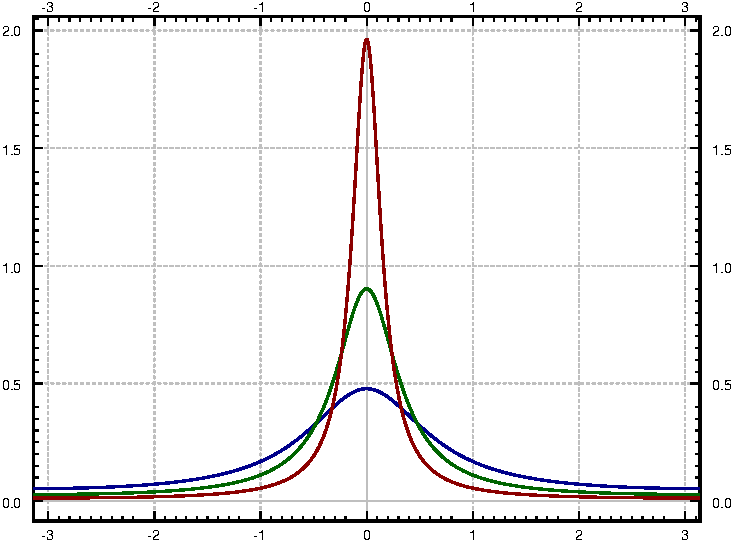
\includegraphics[width=0.5\textwidth]{figures/poisson-kernel.pdf}
\caption{The graph of $P_r$ as a function of $\theta$ on $[-\pi,\pi]$ for
$r=0.5$, $r=0.7$, and $r=0.85$.\label{fig:poissongraph}}
\end{myfig}

\begin{proof}
The first item follows because $1-r^2$ is always positive if $0 \leq r < 1$,
and similarly
\begin{equation*}
1+r^2-2r \cos\theta \geq 1+r^2-2r = {(1-r)}^2 > 0 .
\end{equation*}
Next, denote by $r\D$ the disc of radius $r$ around $0$,
\begin{equation*}
\begin{split}
\int_{-\pi}^{\pi}
P_r(\theta) \, d\theta
& =
\frac{1}{2\pi}
\int_{-\pi}^{\pi}
\Re
\left(
\frac{1+re^{i\theta}}{1-re^{i\theta}}
\right)
\, d\theta
\\
& =
\Re
\frac{1}{2\pi i}
\int_{-\pi}^{\pi}
\frac{1+re^{i\theta}}{1-re^{i\theta}} \frac{1}{re^{i\theta}} \,
ire^{i\theta}
\, d\theta
\\
& = 
\Re
\frac{1}{2\pi i}
\int_{\partial r\D}
\frac{(1+z)/(1-z)}{z} \, dz
=
\Re \frac{1+0}{1-0} = 1 .
\end{split}
\end{equation*}
The last equality follows by the Cauchy integral formula
using the function $\frac{1+z}{1-z}$ evaluated at $0$.

For the third item, notice that we only need to prove the
theory for $\delta \leq \theta \leq \pi$ by symmetry ($P_r$ is even).
On $(0,\pi)$, $P_r$ is strictly decreasing as $\cos \theta$ is strictly
increasing.  So we only need to show that $P_r(\delta)$ goes to $0$
as $r \to 1$ if $\delta > 0$.
This follows by noting that $r \mapsto
\frac{1+re^{i\delta}}{1-re^{i\delta}}$
is continuous at $r=1$ and
\begin{equation*}
\frac{1+e^{i\delta}}{1-e^{i\delta}}
=
\frac{(1+e^{i\delta})(1-e^{-i\delta})}{(1-e^{i\delta})(1-e^{-i\delta})}
=
\frac{e^{i\delta}-e^{i\delta}}{\sabs{1-e^{i\delta}}^2}
=
i \frac{2\Im e^{i\delta}}{\sabs{1-e^{i\delta}}^2}
\end{equation*}
is purely imaginary.
\end{proof}

\begin{thm} \label{thm:dirichsol}
Let $u \colon \partial \D \to \R$ be a continuous function.
The function
$Pu \colon \overline{\D} \to \R$, defined by
\glsadd{not:Pu}%
\begin{equation*}
Pu(re^{i\theta})
=
\int_{-\pi}^\pi u(e^{it}) P_r(\theta-t) \, dt
\quad \text{if $r < 1$} \qquad \text{and} \qquad
Pu(e^{i\theta}) = u(e^{i\theta}),
\end{equation*}
is harmonic in $\D$ and continuous on $\overline{\D}$.
\end{thm}

\begin{proof}
Let $z = re^{i\theta}$.
Then for any fixed $t$,
\begin{equation*}
P_r(\theta-t)
=
\frac{1}{2\pi}
\Re
\left(
\frac{1+re^{i(\theta-t)}}{1-re^{i(\theta-t)}}
\right) 
%=
%\frac{1}{2\pi}
%\Re
%\left(
%\frac{1+re^{i\theta}e^{-it}}{1-re^{i\theta}e^{-it}}
%\right)
=
\frac{1}{2\pi}
\Re
\left(
\frac{1+ze^{-it}}{1-ze^{-it}}
\right)
\end{equation*}
is harmonic as a function of $z=re^{i\theta}$.
By differentiating under the integral,
\begin{equation*}
Pu(z)
=
Pu(re^{i\theta})
=
\int_{-\pi}^\pi u(e^{it}) P_r(\theta-t) \, dt
=
\frac{1}{2\pi}
\int_{-\pi}^\pi u(e^{it}) 
\Re
\left(
\frac{1+z e^{-it}}{1-z e^{-it}}
\right) 
\, dt
\end{equation*}
is harmonic for $z = re^{i\theta} \in \D$.

Now as both $P_r$ and $u(e^{it})$ is $2 \pi$-periodic we 
can change variables:
\begin{equation*}
Pu(re^{i\theta})
=
\int_{-\pi}^\pi u(e^{it}) P_r(\theta-t) \, dt
=
\int_{-\pi}^\pi u\bigl(e^{i(\theta-t)}\bigr) P_r(t) \, dt .
\end{equation*}

Suppose $M$ is the supremum of
$u$ on $\partial \D$.  Suppose $\epsilon > 0$ is given.
As $u$ is uniformly continuous on $\partial \D$, suppose $\delta > 0$
is small enough so that $\sabs{u\bigl(e^{i(\theta-t)}\bigr)-u(e^{i\theta})} <
\frac{\epsilon}{2}$ whenever $\sabs{t} < \delta$.
Using the proposition above, for $r < 1$ large enough, say
$r > 1-\delta'$ for some $\delta'$,
we get $0 < P_r(t) < \frac{\epsilon}{8M\pi}$
whenever $\sabs{t} \geq \delta$.

Using the fact that
$\int_{-\pi}^\pi P_r(t) \, dt = 1$,
we have\footnote{This is a trick you see all over in analysis, it is good to
remember it.} that
\begin{equation*}
u(e^{i\theta})=
\int_{-\pi}^\pi u(e^{i\theta}) P_r(t) \, dt ,
\end{equation*}
so
\begin{equation*}
\begin{split}
\sabs{
Pu(r e^{i\theta} ) - u(e^{i\theta})
}
& =
\abs{
\int_{-\pi}^{\pi} \Bigl( u\bigl(e^{i(\theta-t)}\bigr)-u(e^{i\theta}) \Bigr) P_r(t) \, dt
}
\\
& \leq 
\abs{
\int_{-\pi}^{-\delta} \cdots \, dt
}
+
\abs{
\int_{-\delta}^{\delta} \cdots \, dt
}
+
\abs{
\int_{\delta}^\pi \cdots \, dt
} .
\end{split}
\end{equation*}
Let us estimate the three integrals.
First suppose $M$ is the supremum of
$u$ on $\partial \D$.  So
\begin{equation*}
\begin{split}
\abs{
\int_{-\pi}^{-\delta} \Bigl( u\bigl(e^{i(\theta-t)}\bigr)-u(e^{i\theta}) \Bigr) P_r(t) \, dt
}
& \leq
\int_{-\pi}^{-\delta} \abs{ u\bigl(e^{i(\theta-t)}\bigr)-u(e^{i\theta}) }
P_r(t) \, dt
\\
& \leq (\pi-\delta) 2M \frac{\epsilon}{8M\pi} \leq \frac{\epsilon}{4} .
\end{split}
\end{equation*}
The integral from $\delta$ to $\pi$ is exactly the same.
Next the middle integral,
\begin{equation*}
\begin{split}
\abs{
\int_{-\delta}^{\delta} \Bigl( u\bigl(e^{i(\theta-t)}\bigr)-u(e^{i\theta}) \Bigr) P_r(t) \, dt
}
& \leq
\int_{-\delta}^{\delta} \abs{u\bigl(e^{i(\theta-t)}\bigr)-u(e^{i\theta})}
P_r(t) \, dt
\\
& \leq
\int_{-\delta}^{\delta} \frac{\epsilon}{2} P_r(t) \, dt
\leq
\int_{-\pi}^{\pi} \frac{\epsilon}{2} P_r(t) \, dt
=\frac{\epsilon}{2} .
\end{split}
\end{equation*}
Putting it all together, as long as $1-\delta' < r < 1$,
\begin{equation*}
\sabs{
Pu(r e^{i\theta} ) - u(e^{i\theta})
} \leq \frac{\epsilon}{4} + \frac{\epsilon}{2} + \frac{\epsilon}{4} =
\epsilon.
\end{equation*}
And so $Pu(re^{i\theta}) \to u(e^{i\theta})$ uniformly in $\theta$
as $r \uparrow 1$.

Finally, we must show that for any $z_0 = e^{i\theta_0} \in \partial \D$
we have that
$Pu(z)$ tends to $Pu(z_0)=u(z_0)$ as $z \in \overline{\D}$ tends to $z_0$.
Let $\epsilon > 0$ be given.  As $u = Pu|_{\partial \D}$ is
continuous, pick a $\delta > 0$ such that
$\sabs{Pu(e^{i\theta})-Pu(e^{i\theta_0})} < \frac{\epsilon}{2}$
whenever $\sabs{\theta-\theta_0} < \delta$.
Also make $\delta$ small enough so that $\sabs{Pu(re^{i
\theta})-Pu(e^{i\theta})} < \frac{\epsilon}{2}$
when $1 - \delta < r \leq 1$ for all $\theta$.
Putting the two estimates together we get 
$\sabs{Pu(re^{i\theta})-Pu(e^{i\theta_0})} < \epsilon$, and so $Pu$ is
continuous at $z_0$.
\end{proof}

We remark that in the proof we used the topology on $\overline{\D}$
given by the polar coordinates, and we estimated the coordinates separately.
Polar coordinates give a nice local homemorphism
(a continuous bijective map with a continuous inverse) at least outside of
the origin, which is sufficient for us as we only needed to worry about points
on or near the boundary of $\D$.  The reader that is still unconvinced
should write out the details for an exercise.

\begin{exbox}
\begin{exercise}
We proved that given $\epsilon > 0$, there exists a $\delta > 0$ such that
$\sabs{Pu(re^{i\theta})-Pu(e^{i\theta_0})} < \epsilon$
when $\sabs{\theta-\theta_0} < \delta$ and
$1 - \delta < r \leq 1$.  Prove that this really does mean that
$\lim_{z \to z_0} Pu(z) = u(z_0) = Pu(z_0)$.
\end{exercise}
\end{exbox}

It is particularly useful to notice is that
\begin{equation*}
Pu(0) = \frac{1}{2\pi} \int_{-\pi}^{\pi}u(e^{it}) \, dt ,
\end{equation*}
that is $Pu(0)$ is the average value of $u$.  In general, by applying
a scaling and a translation, we find a $Pu$ for a function $u \colon
\partial \Delta_s(p) \to \R$.  We
leave the exact form of the Poisson kernel for $\Delta_s(p)$ as an
exercise, but the averaging phenomenon still holds.  That is,
\begin{equation} \label{eq:averageofPu}
Pu(p) = \frac{1}{2\pi} \int_{-\pi}^{\pi}u(p + s e^{it}) \, dt .
\end{equation}

\begin{exbox}
\begin{exercise}
State and prove a version of \thmref{thm:dirichsol} for an arbitrary disc
$\Delta_r(p)$.  Evaluate at $p$ to prove the averaging identity above.
\end{exercise}

\begin{exercise}
State and prove a version of \thmref{thm:dirichsol} for a function that is
bounded on $\partial \D$, and continuous at all but finitely many points on
$\partial \D$.  The conclusion should of course be then that $Pu(z)$ ($z \in
\D$) tends
to $u(z_0)$ ($z_0 \in \D$) only if $u$ is continuous at $z_0$.
Note: More advanced students should note that one does not need boundedness,
just $L^1(\partial \D)$ with continuity of $Pu$ wherever $u$ is continuous.
\end{exercise}

\begin{exercise}
\begin{exparts}
\item (Easy)
Dirichlet problem on the upper half-plane $\bH = \{ z \in \C : \Im z > 0 \}$
does not have a unique solution.  Show that $f(z) = c \Im z$ is harmonic for
any $c \in \R$ and $f = 0$ on the real line $\R = \partial \bH$.
\item 
Use the previous exercise to show that the Dirichlet problem has a unique
solution on $\bH$ for a bounded continuous $u$ on $\partial \bH$.
Note: Again, less than bounded is
necessary, but it is sufficient for the exercise.
\end{exparts}
\end{exercise}

\begin{exercise}
Derive the \emph{\myindex{Schwarz integral formula}}, which recovers
a holomorphic function out of the real parts of the boundary values
and the value of the imaginary part at one point.
If $f \colon \overline{\D} \to \C$ is continuous and holomorphic on
$\D$, then for all $z \in \D$,
\begin{equation*}
f(z) =
\frac{1}{2\pi i}
\int_{\partial \D}
\frac{\zeta+z}{\zeta-z} \frac{\Re f(\zeta)}{\zeta} \, d\zeta
+ i \Im f(0) .
\end{equation*}
\end{exercise}

\begin{exercise}
Prove that given any continuous $f \colon \partial \D \to \C$,
there exists a holomorphic $F \colon \D \to \C$ such that $\Re F$ extends
continuously to $\partial \D$ (agrees with a continuous function on
$\overline{\D}$) and such that $\Re F = \Re f$ on $\partial \D$.
That is, given arbitrary boundary data, we cannot in general find a
holomorphic function with those boundary values, but we can do it at least
for the real part.
\end{exercise}

\begin{exercise}
Let $q_1,q_2,\ldots$ be an enumeration of rational
numbers in $[0,1]$.
\begin{exparts}
\item
Define $\varphi \colon [0,1] \to {\mathbb R}$
by $\varphi(t) = \sum_{j=1}^\infty 2^{-j} \chi_{[q_j,1]}(t)$,
where $\chi_{[q_j,1]}(t) = 1$ if $t \in [q_j,1]$ and
zero otherwise (the indicator function).  Show that
$\varphi$ is discontinuous at every rational number in $(0,1]$,
nondecreasing and bounded (hence Riemann integrable).
\item
Define $\Phi(t) = \int_0^t \varphi(s)\, ds$, show that $\Phi$
is increasing, continuous, but not differentiable
on a dense set in $[0,1]$.  Use it to construct a
$\psi(t)$ that is $2\pi$-periodic, continuous and 
not differentiable on a dense subset of $\R$.
\item
Find a continuous $u \colon \overline{\D} \to \R$
such that $u|_{\D}$ is harmonic and
$u(e^{it}) = \psi(t)$, then find a holomorphic $h \colon \D \to \C$
such that $\Re h = u$.
\item
Show that $h$ does not extend through any point of
the boundary, that is for every
$z_0 \in \partial \D$ and every neighbourhood
$U$ of $z_0$, there exists no holomorphic $f \colon U \to \C$
such that $f = h$ on $\D \cap U$.
\end{exparts}
\end{exercise}
\end{exbox}

\subsection{Mean-value property}

The Poisson kernel is also used as a reproducing kernel for
holomorphic functions, as holomorphic functions are harmonic (their real and
imaginary parts are).
A Poisson kernel also exists for higher dimensions, and has
analogous properties.
The solution to the Dirichlet problem using the Poisson kernel leads to
the following proposition.

\begin{thm}[Mean-value property]
\label{prop:meanprop}
\index{mean-value property}
Let $U \subset \C$ be an open set.
A continuous function
$f \colon U \to \R$
is harmonic if and only if 
\begin{equation*}
f(p) = \frac{1}{2\pi} \int_{-\pi}^{\pi} f(p+re^{i\theta})\, d\theta
\qquad \text{whenever} \quad
\overline{\Delta_r(p)} \subset U .
\end{equation*}
\end{thm}

\begin{proof}
One direction is simple.  Suppose that $f$ is harmonic and
$\overline{\Delta_r(p)} \subset U$.  Solve the
Dirichlet problem in $\Delta_r(p)$ using the Poisson kernel
given the boundary values
$f|_{\partial \Delta_r(p)}$.  Using \eqref{eq:averageofPu} and the
uniqueness of the solution of the Dirichlet problem, we find
\begin{equation*}
f(p) = P\bigl[f|_{\partial \Delta_r(p)}\big](p) =
\frac{1}{2\pi} \int_{-\pi}^{\pi}f(p + r e^{it}) \, dt .
\end{equation*}

For the other direction, suppose $f$ is continuous and satisfies the
mean-value property.  Let $\overline{\Delta_r(p)} \subset U$ be an
arbitrary closed disc.  Let $h = P\bigl[f|_{\partial \Delta_r(p)}\big]$
be the solution of the Dirichlet problem in $\Delta_r(p)$ with boundary
values given by $f$.  Consider $\varphi = f-h$,
which is continuous, identically zero
on $\partial \Delta_r(p)$ and still satisfies the mean-value property
on every closed disc in $U$.  Suppose for contradiction that $\varphi$ is positive
somewhere on $\Delta_r(p)$, let $\varphi$ achieve a maximum at $q \in
\Delta_r(p)$.
The set $S \subset \overline{\Delta_r(p)}$ where $\varphi(z) = \varphi(q)$ is compact.
We could thus assume that $q$ is the point closest to
$\partial \Delta_r(p)$.  For some small $s$ the circle
$\partial \Delta_s(q) \subset \Delta_r(q)$ and for some neighborhood
of $\partial \Delta_s(q)$ the function $\varphi$ must be less than some fixed
negative constant.  See \figureref{fig:meanvalue}.

\begin{myfig}
%Note this figure is used later as well
\subimport*{figures/}{meanvalue.pdf_t}
\caption{The discs $\Delta_r(p)$ and $\Delta_s(q)$ and the set
$S$.\label{fig:meanvalue}}
\end{myfig}

In particular, we obtain the strict inequality
\begin{equation*}
\frac{1}{2\pi} \int_{-\pi}^{\pi} \varphi(p+re^{i\theta})\, d\theta <
\varphi(q) .
\end{equation*}
Which is a contradiction as $\varphi$ was still supposed to satisfy the
mean-value property.

We have proved that $\varphi \leq 0$ on $\Delta_r(p)$.  By applying the same
logic to $-\varphi$ we find that $\varphi = 0$ on $\Delta_r(p)$.  In
particular, we find that $f=h$ and $h$ is harmonic, so $f$ is harmonic.
\end{proof}

The Poisson kernel and so the Poisson integral easily applies to any disc
$\Delta_r(p)$ by translation and dilation.  See the exercises.
The uniqueness of the Dirichlet problem says that if $f \colon U \to \R$
is harmonic and $\overline{\Delta_r(p)} \subset U$, then applying
Poisson integral on the disc says that $P\bigl[f|_{\partial
\Delta_r(p)}\bigr] = f$ on $\Delta_r(p)$.  So the Poisson integral gives
a representation of harmonic functions in terms of boundary values, just
like the Cauchy integral formula does for holomorphic functions.

\begin{exbox}
\begin{exercise}
Prove the maximum principle for harmonic functions directly from the
mean-value property.
\end{exercise}

\begin{exercise} \label{exercise:meanvaluesmallronly}
%FIXME: needed
It is not necessary to assume the mean-value property for all discs.  Prove
that given a continuous $f$ as in the theorem such that for every $p \in U$
there is an $s > 0$ (depending on $p$) such that $f$ satisfies the mean-value
property on all discs $\Delta_r(p)$ for every $r < s$, then $f$ is
harmonic.
\end{exercise}
\end{exbox}

\subsection{Harnack's inequality}

Just like holomorphic functions, harmonic functions that are defined in a
disc cannot just do what they want inside the disc, and their behavior is
somewhat controlled by the size of the disc.  That is, the further
``inside'' their domain of definition they live, the more control one has.
The basic example of this is \emph{\myindex{Harnack's inequality}}.

\begin{thm}[Harnack]
Suppose $f \colon \Delta_R(p) \to \R$ is harmonic and nonnegative.
Suppose $z \in \Delta_R(p)$ with $\sabs{z-p} = r$.  Then
\begin{equation*}
\frac{R-r}{R+r} f(p) \leq f(z) \leq \frac{R+r}{R-r} f(p) .
\end{equation*}
\end{thm}

\begin{proof}
FIXME
\end{proof}

There is also the general Harnack inequality in any domain.

\begin{cor}[Harnack]
Suppose $U \subset \C$ is a domain.  Then there exists a $C > 0$ such
that
\begin{equation*}
\sup_{z \in U} f(z) \leq C \inf_{z\in U} f(z)
\end{equation*}
for every harmonic and nonnegative function $f$ defined on $U$.
\end{cor}

FIXME

\subsection{Harnack's theorem}

FIXME?

\begin{thm}
FIXME: convergence?
\end{thm}

FIXME: Montel?

%FIXME: maybe just skip for now
%\subsection{Hopf lemma}
%
%FIXME: do Hopf lemma in a disc

%%%%%%%%%%%%%%%%%%%%%%%%%%%%%%%%%%%%%%%%%%%%%%%%%%%%%%%%%%%%%%%%%%%%%%%%%%%%%%

\section{Extending harmonic functions}

\subsection{Removable isolated singularities}

For harmonic functions we get the following classification of removable
singularities, which is sharp in fact.  That is, the harmonic function $\log
\sabs{z}$ has a nonremovable singularity at the origin, but any function
that blows up any slower than that, doesn't actually blow up and is in fact
harmonic.

\begin{thm}
Suppose $U \subset \C$ is open, $p \in U$, and $f \colon U \setminus \{ p \}
\to \R$ is harmonic such that
\begin{equation*}
\lim_{z\to p} \frac{f(z)}{\log \sabs{z}} = 0 .
\end{equation*}
Then there exists a harmonic $\tilde{f} \colon U \to \R$ such that
$f = \tilde{f}$ on $U \setminus \{ p \}$.
\end{thm}

\begin{proof}
By considering $f(a z + b)$ we may assume, without loss of generality,
that $p = 0$ and $\overline{D} \subset U$.  Solve the Dirichlet problem
$\nabla^2 u = 0$
in $\D$ with boundary data $u|_{\partial \D} = f|_{\partial \D}$.
We wish to show that $u$ equals $f$ in $\D \setminus \{0\}$.
The function
$g = f - u$ is harmonic in $\D \setminus \{ 0 \}$ and it is zero on
$\partial \D$.  We furthermore have that
\begin{equation*}
\lim_{z \to 0} \frac{g(z)}{-\log \sabs{z}} = 0
\end{equation*}
or in other words, given any $\epsilon > 0$, then
in some closed disc $\overline{\Delta_\delta(0)}$ we have
\begin{equation} \label{eq:removableestimateharmonic}
-\epsilon (- \log\sabs{z})
\leq
g(z)
\leq
\epsilon (- \log\sabs{z}) .
\end{equation}
The estimate \eqref{eq:removableestimateharmonic} holds also when
$\sabs{z}=1$.
The function $-\log\sabs{z}$ is harmonic outside of the origin, so
using the maximum principle we have that
\eqref{eq:removableestimateharmonic} holds also for $\delta \leq \sabs{z}
\leq 1$.  As $\epsilon$ was arbitrary we get that $g(z) = 0$ for all
$z \in \D \setminus \{0\}$, and so $u$ is the extension we are looking for.
\end{proof}

\begin{exbox}
\begin{exercise}
Prove that the Dirichlet problem is not solvable in the punctured disc $\D
\setminus \{ 0 \}$.
\end{exercise}
\end{exbox}

\subsection{Schwarz reflection principle}

Classically, the Schwarz reflection principle is a theorem for holomorphic
functions, but we will state and prove it for harmonic functions.
We will prove the corresponding holomorphic version
(\thmref{thm:schwarzreflectionholo}) later separately.

Basically it says that if a harmonic function vanishes on a nice enough
curve (such as the real line) then it extends across.

\begin{thm}[Schwarz reflection principle for harmonic functions]
\index{Schwarz reflection principle!harmonic functions}
\label{thm:schwarzreflectionharm}
Suppose $U \subset \C$ is a domain symmetric across the real axis, that is,
$z \in U$ if and only if $\bar{z} \in U$.
Let $U_+ = \{ z \in U : \Im z > 0 \}$ and $L = U \cap \R$.
Suppose $f \colon U_+ \cup L \to \R$ be continuous function that is
harmonic on $U_+$ and $f(z) = 0$ for all $z \in L$.

Then there exists a harmonic $F \colon U \to \R$ such that
$F|_{U_+ \cup L} = f$.
\end{thm}

FIXME: needs a figure

\begin{proof}
The trick is to explicitly define what we want the function to be and then
check that it is harmonic.
For $z \in U$ define
\begin{equation*}
F(z) =
\begin{cases}
f(z) & \text{if } \Im z \geq 0, \\
-f(\bar{z}) & \text{else} .
\end{cases}
\end{equation*}

If $z \in U$ and $\Im z > 0$, then $F$ is harmonic at $z$ by hypothesis.
Suppose $z \in U$ and $\Im z < 0$.  Write $F(z) = F(x,y) = -f(x,-y)$, then
\begin{equation*}
\nabla^2|_{(x,y)} F
=
\nabla^2|_{(x,y)} \bigl( -f(x,-y) \bigr)
=
- \frac{\partial^2 f}{\partial x^2}|_{(x,-y)}
- \frac{\partial^2 f}{\partial y^2}|_{(x,-y)}
=
- \nabla^2|_{(x,-y)} f = 0 .
\end{equation*}
So suppose that $z \in L$, that is, $z \in \R$.
Let us compute the mean value at $z$ around any
$\partial \Delta_r(z)$ where $\overline{\Delta_r(z)} \subset U$:
\begin{equation*}
\frac{1}{2\pi} \int_{-\pi}^{\pi} F(z+re^{i\theta})\, d\theta
=
\frac{1}{2\pi} \int_{-\pi}^{0} -f(z+re^{-i\theta})\, d\theta
+
\frac{1}{2\pi} \int_{0}^{\pi} f(z+re^{i\theta})\, d\theta
=
0 .
\end{equation*}
In other words the mean value equals $F(z) = 0$.
So the mean-value property is satisfied for all small enough
$r$ at all the $z \in L$.  The mean-value property
is also satisfied for small enough
$r$ around any other point since $F$ is harmonic on the open set $U
\setminus L$.
Thus, by \exerciseref{exercise:meanvaluesmallronly}, $F$ is harmonic in $U$.
\end{proof}

FIXME:


%%%%%%%%%%%%%%%%%%%%%%%%%%%%%%%%%%%%%%%%%%%%%%%%%%%%%%%%%%%%%%%%%%%%%%%%%%%%%%

\section{Subharmonic functions}
\label{sec:subharmonic}

Holomorphic, and hence harmonic, functions are very rigid.
There is a less restrictive (and much larger) set of functions that allows
us to study harmonic functions.  In essence, we replace equalities, which are
hard to solve, by inequalities, which are much easier to work with.

\subsection{Basic properties}

\begin{defn}
Let $U \subset \C$ be open.
A function $f \colon U \to \R \cup \{ -\infty \}$ is 
\emph{\myindex{subharmonic}} if it is upper-semicontinuous (see below)
and for every
disc $\Delta_r(p)$ with $\overline{\Delta_r(p)} \subset U$,
and every continuous $g \colon \overline{\Delta_r(p)} \to \R$,
harmonic on $\Delta_r(p)$,
such that $f(z) \leq g(z)$ for $z \in \partial \Delta_r(p)$, we have
\begin{equation*}
f(z) \leq g(z) \quad \text{ for all } z \in \Delta_r(p) .
\end{equation*}

Recall that $f \colon U \to \R \cup \{ -\infty \}$
is \emph{\myindex{upper-semicontinuous}}
if 
\begin{equation*}
\limsup_{\zeta \to z} f(\zeta) \leq f(z) \quad \text{ for all } z \in U.
\end{equation*}
\end{defn}

In other words, a subharmonic function is a function that is less than every
harmonic function on every disc.

The best way to think about subharmonic functions is an analogy to convex
functions.
We could make similar definitions of harmonic and subharmonic
in $\R$ rather than $\C$ (in fact one can and often does make these
definitions in $\R^n$ for any $n$).
In this case (in $\R$ that is), a function $g(x)$ is harmonic if
$\frac{\partial^2}{\partial x^2} g = g'' = 0$, that is, $g(x) = Ax+B$, an affine
linear function.
A function of one real variable is
\emph{convex}\index{convex function} if 
for every interval it is less than the affine linear function with the same
end points.
That is,
the function $f$ is convex if on
every interval $[\alpha,\beta]$, $f \leq g$ for every affine linear $g$
bigger than $f$ at the endpoints $\alpha$ and $\beta$.
An interval $[\alpha,\beta]$ plays the role of a closed disc in $\R$.
In particular, we can take the $g$ that is equal to $f$ at the endpoints.

So \emph{convex} is the same as \emph{subharmonic} in
$\R$.
Graphs of real-valued functions of one real variable
are also much easier to draw than functions on $\C$, see
\figureref{fig:convexfunc}.

\begin{myfig}
\subimport*{figures/}{convexfunc.pdf_t}
\caption{A convex function.\label{fig:convexfunc}}
\end{myfig}

\begin{exbox}
\begin{exercise}
%FIXME: mark needed/used exercises
Prove that given an upper-semicontinuous function $f \colon U \to \R \cup
\{-\infty\}$,
the set $S = f^{-1}\bigl([a,\infty)\bigr) = \{ z \in U : f(z) \geq a \}$
is closed (in the subspace topology of $U$).
\end{exercise}

\begin{exercise}
%FIXME: mark needed/used exercises
Prove that an upper-semicontinuous function achieves a maximum on compact sets.
\end{exercise}

\begin{exercise}
Prove that if $f \colon U \to \R$ is upper-semicontinuous and $-f$ is also
upper-semicontinuous (that is $f$ is also lower-semicontinuous), then $f$
is continuous.
\end{exercise}
\end{exbox}

A useful property that we will use often is that adding or subtracting 
harmonic functions does not kill subharmonicity.  The proof is rather simple
as a sum or difference of harmonic functions is harmonic and we leave it as
an exercise.

\begin{prop} \label{prop:fplushsubharmonic}
If $f \colon U \to \R \cup \{ - \infty \}$ is subharmonic and $h \colon U
\to \R$ is harmonic, then $f+h$ is subharmonic.
\end{prop}

\begin{exbox}
\begin{exercise}
Prove the proposition.
\end{exercise}
\end{exbox}

Suharmonic functions are also classified by a mean value like property,
although it is an inequality rather than an equality.  There is a subtle
issue of integrability however.
We will only prove this for the upper Darboux integral.
The proof is 
similar for the Lebesgue integral if the reader knows that, although
the statement with the Darboux integral is sufficient for us.

\begin{prop}[Sub-mean-value property]
\label{prop:submeanprop}
\index{sub-mean-value property}
Let $U \subset \C$ be an open set.
An upper-semicontinuous function $f \colon U \to \R \cup \{ -\infty \}$
is subharmonic if and only if
\begin{equation*}
f(p) \leq \frac{1}{2\pi} \int_{-\pi}^{\pi} f(p+re^{i\theta})\, d\theta
\qquad \text{whenever} \quad
\overline{\Delta_r(p)} \subset U .
\end{equation*}
The integral is either the Lebesgue integral or the upper Darboux integral,
the function need not be Riemann integrable.
\end{prop}

As $\partial \Delta_r(p)$ is compact and $f$ is upper-semicontinuous, then
$f$ is bounded from above and hence the upper Darboux integral is defined
and finite.
The upper Darboux integral of a function $f$ on $[a,b]$ bounded above is normally defined as
\begin{equation*}
\overline{\int_a^b} f(t) \,dt
\overset{\text{def}}{=}
\inf \left\{ \int_a^b s(t) \, dt : s
\text{ is a step function and } s(t) \geq f(t) \text{ for } t \in
[a,b] \right\}
\end{equation*}
A step function is a finite sum of characteristic functions of intervals and
hence Riemann integrable.
Since continuous functions are Riemann integrable we can approximate from
above by continuous functions $g$ such that
$\int_a^b g(t)\,dt$
approximates
$\int_a^b s(t)\,dt$.  In other words, in the definition we could replace
step functions with continuous functions, and that is what we will use in
the proof.

\begin{proof}
First suppose that $f$ is subharmonic and fix a closed disc
$\overline{\Delta_r(p)} \subset U$.
Fix $\epsilon > 0$.
Find a continuous function $g \colon \partial \Delta_r(p) \to \R$
such that $f(p+ re^{i\theta}) \leq g(p+re^{i\theta})$ for all $\theta$
and such that
\begin{equation*}
\frac{1}{2\pi} \int_{-\pi}^{\pi} g(p+re^{i\theta})\, d\theta <
\frac{1}{2\pi} \overline{\int_{-\pi}^{\pi}} f(p+re^{i\theta})\, d\theta + \epsilon .
\end{equation*}
Solve the Dirichlet problem in the disc $\Delta_r(p)$ for $g$ and
in a slight abuse of notation call the solution on $\overline{\Delta_r(p)}$
also $g$.  As $g$ is harmonic and bigger than $f$ we have by
definition of subharmonicity and the mean-value property of harmonic
functions
\begin{equation*}
f(p) \leq g(p) =
\frac{1}{2\pi} \int_{-\pi}^{\pi} g(p+re^{i\theta})\, d\theta <
\frac{1}{2\pi} \overline{\int_{-\pi}^{\pi}} f(p+re^{i\theta})\, d\theta + \epsilon .
\end{equation*}

Now suppose conversely that the estimate always holds and $f$ is upper
semicontinuous.  We will prove the contrapositive.  Suppose that $f$ is not
subharmonic.  Then there exists a closed disc 
$\overline{\Delta_r(p)} \subset U$ and a continuous
$h \colon \overline{\Delta_r(p)} \to \R$, harmonic in $\Delta_r(p)$,
such that $f(z) \leq h(z)$ on $\partial \Delta_r(p)$ and
$h(q) < f(q)$ at some point $q \in \Delta_r(p)$.
Let $\varphi = f-h$, then $\varphi(q) > 0$ and $\varphi(z) \leq 0$
for all $z \in \partial \Delta_r(p)$.  The set
$S \subset \overline{\Delta_r(p)}$ where $\varphi(z) = \varphi(q)$ is closed and so
compact (via an exercise above).
We could thus assume that $q$ is the point closest to
$\partial \Delta_r(p)$.  In this case for some small $s$ the circle
$\partial \Delta_s(q) \subset \Delta_r(q)$ and for some neighborhood
of $\partial \Delta_s(q)$ the function $\varphi$ must be less than some fixed
nnegative constant.  The setup is the same as in \figureref{fig:meanvalue}.

In particular we obtain the strict inequality
\begin{equation*}
\frac{1}{2\pi} \overline{\int_{-\pi}^{\pi}} \varphi(p+re^{i\theta})\, d\theta <
\varphi(q) . \qedhere
\end{equation*}
\end{proof}

From now on, when we apply the property we simply write the integral and
the reader substitutes the upper Darboux integral or the Lebesgue integral
according to the reader's taste.

\begin{exbox}
\begin{exercise}
Let $U \subset \C$ be open.
Show that if $f \colon U \to \R \cup\{- \infty \}$ is subharmonic,
then 
\begin{equation*}
\limsup_{w \to z} f(w) = f(z) 
\qquad \text{for all $z \in U$.}
\end{equation*}
\end{exercise}
\end{exbox}

\begin{prop}[Maximum principle]
\index{maximum principle!subharmonic functions}
Suppose $U \subset \C$ is a domain and $f \colon U \to \R \cup \{ -\infty \}$
is subharmonic.  If $f$ attains a maximum in $U$, then $f$ is constant.
\end{prop}

\begin{proof}
Suppose $f$ attains a maximum at $p \in U$.
If
$\overline{\Delta_r(p)} \subset U$, then
\begin{equation*}
f(p) \leq \frac{1}{2\pi} \int_{-\pi}^{\pi} f(p+re^{i\theta})\, d\theta \leq f(p)
.
\end{equation*}
Hence, $f = f(p)$ almost everywhere on $\partial \Delta_r(p)$.
By upper-semicontinuity, $f = f(p)$ everywhere on $\partial \Delta_r(p)$.
This was true for all $r$
with $\overline{\Delta_r(p)} \subset U$, so $f=f(p)$ on $\Delta_r(p)$,
and so the set where $f=f(p)$ is open.  The set where an upper-semicontinuous
function attains a maximum is closed.  So $f=f(p)$ on $U$ as $U$ is
connected.
\end{proof}

\begin{exbox}
\begin{exercise}
Prove that subharmonicity is a local property.  That is, given an open set
$U \subset \C$, a function $f \colon U \to \R \cup \{ -\infty \}$ is subharmonic if
and only if for every $p \in U$ there exists a neighborhood $W$ of $p$,
$W \subset U$, such that $f|_{W}$ is subharmonic.  Hint: Perhaps try to use
the maximum principle and \propref{prop:fplushsubharmonic}.
\end{exercise}

\begin{exercise}
Suppose $U \subset \C$ is a bounded open set, $f \colon \overline{U} \to \R
\cup \{-\infty\}$ is an upper-semicontinuous function, such that $f|_U$
is subharmonic, $g \colon \overline{U} \to \R$ is a continuous function
such that $g|_U$ is harmonic and
$f(z) \leq g(z)$ for all $z \in \partial U$.  Prove that
$f(z) \leq g(z)$ for all $z \in U$.
\end{exercise}

\begin{exercise} \label{exercise:onlyniceuneededforsubharmonic}
Let $g$ be a function
harmonic on a disc $\Delta \subset \C$ and continuous on
$\overline{\Delta}$.  Prove that for every $\epsilon > 0$ there exists
a function $g_\epsilon$, harmonic in a neighborhood of $\overline{\Delta}$,
such that $g(z) \leq g_\epsilon(z) \leq g(z)+\epsilon$ for all $z \in
\overline{\Delta}$.
In particular, to test subharmonicity, we only need to consider those
$g$ that are harmonic a bit past the boundary of the disc.
\end{exercise}
\end{exbox}

\begin{prop}
Suppose $U \subset \C$ is an open set and $f \colon U \to \R$ is a $C^2$
(twice continuously differentiable) function.
The function $f$ is subharmonic if and only if
$\nabla^2 f \geq 0$.
\end{prop}

\begin{proof}
Suppose $f$ is a $C^2$-smooth function on a subset of $\C \cong \R^2$
with $\nabla^2 f \geq 0$.  We wish to show that $f$ is subharmonic.
Take a disc $\Delta$ such that $\overline{\Delta} \subset U$.
Consider a function
$g$ continuous on $\overline{\Delta}$,
harmonic on $\Delta$, and such that
$f \leq g$ on the boundary $\partial \Delta$.  Because
$\nabla^2 (f-g) = \nabla^2 f \geq 0$, we assume $g = 0$ and $f \leq 0$
on the boundary $\partial \Delta$. 

Suppose $\nabla^2 f > 0$ at all points on $\Delta$.
Suppose $f$ attains a maximum in $\Delta$,
call this point $p$.  
The Laplacian $\nabla^2 f$ is the trace of the Hessian matrix, but for $f$ to have a
maximum, the Hessian must have only nonpositive eigenvalues at the critical
points, which is a
contradiction as the trace is the sum of the eigenvalues.  So $f$ has no
maximum inside, and therefore $f \leq 0$ on all of
$\overline{\Delta}$.

Next suppose $\nabla^2 f \geq 0$.
Let $M$ be the maximum of $x^2+y^2$ on $\overline{\Delta}$.
Take $f_n(x,y) = f(x,y) + \frac{1}{n}
( x^2+y^2 ) - \frac{1}{n}M$.  Clearly $\nabla^2 f_n > 0$ everywhere on
$\Delta$ and
$f_n \leq 0$ on the boundary, so $f_n \leq 0$ 
on all of $\overline{\Delta}$.  As $f_n \to f$, we obtain that
$f \leq 0$ on all of $\overline{\Delta}$.

The other direction is left as an exercise.
\end{proof}

\begin{exbox}
\begin{exercise}
Finish the proof of the proposition above.
\end{exercise}
\end{exbox}

In analogy to convex functions, a $C^2$ function $f$ of one
real variable is convex if and only if $f''(x) \geq 0$ for all $x$.

We can also approximate subharmonic functions from above.

\begin{prop}
Suppose $U \subset \C$ is an open set and $f_\alpha \colon U \to \R \cup \{ -\infty \}$
is a family of subharmonic functions.  Let
\begin{equation*}
\varphi(z) = \sup_\alpha\, f_\alpha(z) .
\end{equation*}
If the family is finite, then $\varphi$ is subharmonic.
If the family is infinite, $\varphi(z) \not= \infty$ for
all $z$, and $\varphi$
is upper-semicontinuous, then $\varphi$ is subharmonic.
\end{prop}

\begin{proof}
Suppose $\overline{\Delta_r(p)} \subset U$.  For any $\alpha$,
\begin{equation*}
\frac{1}{2\pi} \int_{-\pi}^{\pi} \varphi (p+re^{i\theta})\, d\theta 
\geq
\frac{1}{2\pi} \int_{-\pi}^{\pi} f_\alpha (p+re^{i\theta})\, d\theta 
\geq f_\alpha(p) .
\end{equation*}
Taking the supremum on the right over $\alpha$ obtains the results.
\end{proof}

\begin{exbox}
\begin{exercise}
Prove that if $\varphi \colon \R \to \R$ is a monotonically increasing
convex function, $U \subset \C$ is an open set, and $f \colon U \to \R$
is subharmonic, then $\varphi \circ f$ is subharmonic.
\end{exercise}

\begin{exercise}
Let $U \subset \C$ be open, $\{ f_n \}$ a sequence of 
subharmonic functions uniformly bounded above on compact subsets, and 
$\{ c_n \}$ a sequence of positive real numbers such that
$\sum_{n=1}^\infty c_n < \infty$.
Prove that $f = \sum_{n=1}^\infty c_n f_n$ is subharmonic.  Make sure to prove
the function is upper-semicontinuous.
\end{exercise}

\begin{exercise}
Suppose $U \subset \C$ is a bounded open set, and $\{ p_n \}$ a sequence of points in
$U$. For $z \in U$, define
$f(z) = \sum_{n=1}^\infty 2^{-n} \log \sabs{z-p_n}$, possibly taking on the
value $-\infty$.
\begin{exparts}
\item
Show that $f$ is a subharmonic function in $U$.
\item
If $U = \D$ and $p_n = \frac{1}{n}$, show that $f$ is discontinuous at $0$
(the natural topology on $\R \cup \{ -\infty \}$).
\item
If $\{ p_n \}$ is dense in $U$, show that $f$ 
is nowhere continuous.
Hint: Prove $f^{-1}(-\infty)$ is a small (but dense) set.
Hint \#2: Integrate the partial sums, and use polar coordinates.
\end{exparts}
\end{exercise}
\end{exbox}

\subsection{Applications, Rad\'o's theorem}

We are often really interested in proving results for harmonic functions,
as we are interested in proving results for holomorphic functions.
However, harmonic functions are very rigid, they cannot be ``put together''
easily.  Furthermore there aren't that many of them.  There are a lot of
subharmonic functions.

As an example of the use of subharmonic functions for
complex analysis,
let us prove the theorem of 
Rad\'o, which is a complementary result to the Riemann extension theorem.
Here on the one hand the function is
continuous and vanishes on the set you wish to extend across, but on the
other hand you know nothing about this set.

\begin{thm}[Rad\'o]\index{Rad\'o's theorem}\label{thm:rado}
Let $U \subset \C$ be open and $f \colon U \to \C$ a continuous
function that is holomorphic on the set where it is nonzero,
\begin{equation*}
U' = \bigl\{ z \in U : f(z) \not= 0 \bigr\} .
\end{equation*}
Then $f$ is holomorphic.
\end{thm}

\begin{proof}
Holomorphicity is local, so
it is enough to prove the theorem for a small disc $\Delta$
such that $f$ is continuous
on the closure $\overline{\Delta}$, let $\Delta'$ be the part of the disc
where $f$ is nonzero.  If $\Delta'$ is empty, then we are done as
$f$ is just identically zero and hence holomorphic.

Let $u$ be the real part of $f$.  On $\Delta'$, $u$ is a harmonic function.
Let $Pu$ be the Poisson integral of $u$ on $\Delta$.  Hence $Pu$
equals $u$ on $\partial \Delta$, and $Pu$ is harmonic in all of $\Delta$.
Consider the function
$Pu(z) - u(z)$ on $\overline{\Delta}$.  The function is zero
on $\partial \Delta$ and it is harmonic on $\Delta'$.  By rescaling $f$
we can without loss of generality assume that $\abs{f(z)} < 1$ for all $z
\in \overline{\Delta}$.  For any $t >0$, the function 
$z \mapsto t \log \abs{f(z)}$ is subharmonic on $\Delta'$ and
upper-semicontinuous on $\overline{\Delta'}$.  Further, it is negative
on $\partial \Delta$.  The function $z \mapsto -t \log \abs{f(z)}$ is
superharmonic (minus a subharmonic function) on $\Delta'$,
lower-semicontinuous on $\overline{\Delta'}$ and positive on $\partial
\Delta$.  On the set $\Delta \setminus \Delta'$ where $f$ is zero, the two functions are $-\infty$ and
$\infty$ respectively.
See \figureref{fig:radosthm}.
Therefore, for all $t > 0$ and 
$z \in \partial \Delta \cup (\Delta \setminus \Delta')$,
we have
\begin{equation} \label{eq:radobound}
t \log \abs{f(z)} \leq Pu(z)-u(z) \leq -t \log \abs{f(z)}  .
\end{equation}
Applying the maximum principle to the subharmonic functions
$z \mapsto t \log \abs{f(z)} - \bigl(Pu(z)-u(z)\bigr)$
and
$z \mapsto t \log \abs{f(z)} - \bigl(u(z)-Pu(z)\bigr)$
shows that 
\eqref{eq:radobound} holds for all $z \in \Delta'$ and all $t > 0$.

\begin{myfig}
\subimport*{figures/}{radosthm.pdf_t}
\caption{Proof of Rad\'o's theorem.\label{fig:radosthm}}
\end{myfig}

Taking the limit
$t \to 0$ shows that $Pu = u$ on $\Delta'$.
Let $W = \Delta \setminus \overline{\Delta'}$.
On $W$, $u=0$ and so $Pu-u$ is harmonic on $W$
and continuous on $\overline{W}$.  Furthermore,
$Pu-u=0$ on $\overline{\Delta'} \cup \partial \Delta$,
and so $Pu-u=0$ on $\partial W$.  By the maximum principle, $Pu=u$ on $W$
and therefore on all of $\overline{\Delta}$.
Similarly, if $v$ is the imaginary part of $f$, then $Pv = v$ on
$\overline{\Delta}$.
In other words, $u$ and $v$ are harmonic on $\Delta$.
As $\Delta$ is simply connected,
let $\tilde{v}$ be the harmonic conjugate of $u$ that equals $v$ at
some point of $\Delta'$.  As $f$ is holomorphic on $\Delta'$,
the harmonic functions $\tilde{v}$ and $v$
are equal the nonempty open subset $\Delta'$ of $\Delta$ and so
they are equal everywhere.  Consequently, $f = u +iv$ is holomorphic on
$\Delta$.
\end{proof}

Another example of the use subharmonic functions is another solution
to the Dirichlet problem.  A solution can be had by considering all the
subharmonic functions that are less than the function given on the boundary.
Then one takes a supremum to obtain a harmonic function.  We will not go
through this technique which is called the \emph{\myindex{Perron method}}.
Clearly that technique would work far better than the Poisson kernel on
more complicated domains.  For example, the Poisson kernel can be computed
on simply connected domains provided we know the Riemann map.  However,
the kernel is difficult to compute in general, and it requires a very nice
boundary to be able to integrate.  The Perron method works much more
generally provided you can construct enough subharmonic functions (which can
afterall be pieced together unlike harmonic functions).

If a solution exists, it clearly must equal to the Perron solution.

\begin{exbox}
\begin{exercise}
Suppose $U \subset \C$ is a domain and
$u \colon \overline{U} \to \R$ is continuous and
harmonic on $U$, then
\begin{equation*}
u(p) = \sup_{v} v(p)
\end{equation*}
where $v$ range over all upper-semicontinuous functions on $\overline{U}$
subharmonic on $U$,
such that $v|_{\partial U} \leq u|_{\partial U}$.
\end{exercise}
\end{exbox}

%%%%%%%%%%%%%%%%%%%%%%%%%%%%%%%%%%%%%%%%%%%%%%%%%%%%%%%%%%%%%%%%%%%%%%%%%%%%%%
%%%%%%%%%%%%%%%%%%%%%%%%%%%%%%%%%%%%%%%%%%%%%%%%%%%%%%%%%%%%%%%%%%%%%%%%%%%%%%
%%%%%%%%%%%%%%%%%%%%%%%%%%%%%%%%%%%%%%%%%%%%%%%%%%%%%%%%%%%%%%%%%%%%%%%%%%%%%%

\chapter{Rational Approximation} \label{ch:runge}

\begin{myquote}
It has been said that man is a rational animal. All my life I have been searching for evidence which could support this.

---Bertrand Russell
\end{myquote}


%%%%%%%%%%%%%%%%%%%%%%%%%%%%%%%%%%%%%%%%%%%%%%%%%%%%%%%%%%%%%%%%%%%%%%%%%%%%%%

\section{Introduction to polynomial approximation}
\label{sec:polyapprox}

In real analysis, you may have seen the very useful
Weierstrass approximation theorem (and more generally the
Stone--Weierstrass approximation theorem), which says that a continuous function
on a compact interval $[a,b]$ can be uniformly approximated by polynomials
of a real variable.  For holomorphic polynomials, that is polynomials in $z$
we have a similar theorem, but for holomorphic functions not
continuous functions.  That makes sense.  After all, uniform limits of
holomorphic functions are holomorphic.

\begin{example}
Let $z = x+iy$.
By Stone--Weierstrass
any continuous function on the closed unit disc $\overline{\D}$
is a uniform limit of a sequence of polynomials
$Q_n(x,y)$ (polynomials of both $x$ and $y$), but only a function that is
holomorphic on $\D$ can be the uniform limit of polynomials
$P_n(z)$ (polynomial of $z$).

More explicitly the function $z \mapsto \bar{z}=x-iy$ is not only a limit of
polynomials in $x$ and $y$, it is a polynomial in $x$ and $y$.  However as
the function is not holomorphic on $\D$, it cannot be a
uniform limit of holomorphic polynomials on $\overline{\D}$.
\end{example}

From now on, all polynomials will be polynomials in $z$, as they were
up until the example above in fact.  So when we say polynomial, it will be
a polynomial in $z$, in other words, a holomorphic polynomial.

A function holomorphic on a disc $\Delta_r(p)$ is limit of the partial sums
of the power series $\sum_{n=0}^m c_n {(z-p)}^n$.  See also
\exerciseref{exercise:polylimits}.  However, suppose we take a function that
is holomorphic on a neighborhood of the square $[-1,1] \times [-1,1]$, say
$f(z) = \frac{1}{(z-1.1)(z+1.1)}$.  If we expand $f$ around any point, the
series will never converge on all of $[-1,1] \times [-1,1]$.  However we can
(exercise below) still find a sequence of polynomials that converge to $f$
on $[-1,1] \times [-1,1]$.

\begin{exbox}
\begin{exercise}
Let 
$f(z) = \frac{1}{(z-1.1)(z+1.1)}$.  Find an explicit (that is, find a
formula for it, do not just prove that it exists) sequence of polynomials
$P_n(z)$
that converges uniformly to $f$ on the square $[-1,1] \times [-1,1]$.
\end{exercise}
\end{exbox}

Sometimes, we are thwarted in polynomial approximation by topology.  For
example, consider $\frac{1}{z}$ on $\partial \D$.  There is no sequence of
polynomials $P_n(z)$ that converge to $\frac{1}{z}$ uniformly on $\partial
\D$.  This follows by \hyperref[thm:rouche]{Rouch\`e} (or
\exerciseref{exercise:convergeboundary} and Cauchy's theorem), see the
following exercise.

\begin{exbox}
\begin{exercise}
For any polynomial $P(z)$, there exists a $z_0 \in \partial \D$ such that
$\babs{P(z_0)-\frac{1}{z_0}} \geq 1$.
\end{exercise}
\end{exbox}

The problem with the unit circle is that it has a hole.  We can approximate
any function holomorphic in a neighbourhood of $\partial \D$ by rational
functions if we allow a pole at $0$.  The function $\frac{1}{z}$ is already
a rational function with a pole at zero.

A polynomial is really just a rational function that has a pole at infinity.
Once we will prove Runge's theorem we will prove that it really is the hole
that is the problem.  We can approximate a holomorphic function
by polynomials on any set whose complement is connected.

%%%%%%%%%%%%%%%%%%%%%%%%%%%%%%%%%%%%%%%%%%%%%%%%%%%%%%%%%%%%%%%%%%%%%%%%%%%%%%

\section{Rational functions and pushing poles}
\label{sec:rational}

Let us first prove rational approximation without any control of the poles.
The key is going to be that we can find a cycle around any compact set $K$
(see \subsectionref{subsec:patharoundK})
so that we can apply Cauchy's integral formula.  Then the Riemann sums of the
integral are the rational functions.

\begin{lemma}
Let $U \subset \C$ be open, $K \subset U$ compact, $f \colon U \to \C$
holomorphic, and $\Gamma$ a cycle in $U$ homologous to zero in $U$
such that $\Gamma \cap K = \emptyset$ and $n(\Gamma;z) = 1$ for all $z \in
K$.  Then for any $\epsilon > 0$, there exists a rational function $R(z)$ with
poles on $\Gamma$ such that $\sabs{f(z)-R(z)} < \epsilon$ for all $z \in K$.
\end{lemma}

\begin{proof}
The hypotheses mean that we can apply Cauchy's integral formula for any $z
\in K$:
\begin{equation*}
f(z) =
\frac{1}{2\pi i}
\int_\Gamma
\frac{f(\zeta)}{\zeta-z} \, d \zeta .
\end{equation*}
The cycle $\Gamma$ is a finite sum of closed piecewise $C^1$ paths.
If we that the Riemann sums of the corresponding to each path
converge uniformly on $K$, then their sum also converges uniformly
and it converges to $f$.

Thus consider just one path $\gamma \colon [0,1] \to U$, and
let $\epsilon > 0$ be given.
The function
\begin{equation*}
(z,t) \mapsto
\frac{f\bigl(\gamma(t)\bigr)}{\gamma(t)-z}
\end{equation*}
is uniformly continuous on the compact set $K \times [0,1]$.  Furthermore,
as $\gamma'$ is bounded, we can find a $\delta > 0$ such that
\begin{equation*}
\abs{
\frac{f\bigl(\gamma(t)\bigr)}{\gamma(t)-z}\gamma'(t)
-
\frac{f\bigl(\gamma(\tau)\bigr)}{\gamma(\tau)-z}\gamma'(t)
} < \epsilon
\end{equation*}
for all $z \in K$ and all $t,\tau \in [0,1]$ such that $\sabs{t-\tau} <
\delta$.
Partition $[0,1]$ into $0 = t_0 < \cdots < t_k = 1$ such that
$t_j-t_{j-1} < \delta$.
Write
\begin{equation*}
\int_\gamma
\frac{f(\zeta)}{\zeta-z} \, d\zeta
=
\sum_{j=1}^k
\int_{t_{j-1}}^{t_j}
\frac{f\bigl(\gamma(t)\bigr)}{\gamma(t)-z}
\gamma'(t)
\, dt .
\end{equation*}
Let us estimate each bit of this integral by a rational function
(note the use of the fundamental theorem of calculus)
\begin{multline*}
\abs{
\int_{t_{j-1}}^{t_j}
\frac{f\bigl(\gamma(t)\bigr)}{\gamma(t)-z}
\gamma'(t)
\, dt
\enspace
-
\enspace
\frac{f\bigl(\gamma(t_j)\bigr)}{\gamma(t_j)-z}
\bigl( \gamma(t_j)-\gamma(t_{j-1}) \bigr)
}
\\
=
\abs{
\int_{t_{j-1}}^{t_j}
\left(
\frac{f\bigl(\gamma(t)\bigr)}{\gamma(t)-z}
\gamma'(t)
-
\frac{f\bigl(\gamma(t_j)\bigr)}{\gamma(t_j)-z}
\gamma'(t)
\right)
\, dt
}
\\
\leq
\int_{t_{j-1}}^{t_j}
\abs{
\frac{f\bigl(\gamma(t)\bigr)}{\gamma(t)-z}
\gamma'(t)
-
\frac{f\bigl(\gamma(t_j)\bigr)}{\gamma(t_j)-z}
\gamma'(t)
}
\, dt
\leq \epsilon (t_j-t_{j-1}) .
\end{multline*}
Summing these bits together and using the triangle inequality, we find
\begin{equation*}
\abs{
\int_{\gamma} \frac{f(\zeta)}{\zeta-z} \, d\zeta
-
\sum_{j=1}^k
\frac{f\bigl(\gamma(t_j)\bigr)}{\gamma(t_j)-z}
\bigl( \gamma(t_j)-\gamma(t_{j-1}) \bigr)
}
\leq \sum_{j=1}^k \epsilon (t_j-t_{j-1}) = \epsilon .
\end{equation*}
Thus the integral over $\gamma$ converges uniformly for $z \in K$, and
we are done by summing up over all the paths in $\Gamma$.
\end{proof}







FIXME

%%%%%%%%%%%%%%%%%%%%%%%%%%%%%%%%%%%%%%%%%%%%%%%%%%%%%%%%%%%%%%%%%%%%%%%%%%%%%%

\section{Runge's theorem}
\label{sec:runge}

FIXME:

\begin{lemma}[Runge on a compact set]\index{Runge on a compact set}
Suppose $U \subset \C$ is open, $K \subset U$ is compact, $S \subset \C_{\infty} \setminus K$
is a set that intersects every component of $\C_\infty \setminus K$,
and $f \colon U \to \C$ is holomorphic.
Then for every $\epsilon > 0$,
there exists a rational function $R$ with poles in $S$ such that
\begin{equation*}
\abs{f(z)-R(z)} < \epsilon \qquad \text{for all $z \in K$.}
\end{equation*}
\end{lemma}

FIXME

\begin{thm}[Runge]\index{Runge's theorem}
Suppose $U \subset \C$ is open, $S \subset \C_{\infty} \setminus U$
is a set that intersects every component of $\C_\infty \setminus U$,
and $f \colon U \to \C$ is holomorphic.
Then there exists a sequence $\{ R_n \}$ of rational functions with poles in $S$
that converges to $f$ uniformly on compact subsets.
\end{thm}

FIXME

%%%%%%%%%%%%%%%%%%%%%%%%%%%%%%%%%%%%%%%%%%%%%%%%%%%%%%%%%%%%%%%%%%%%%%%%%%%%%%

\section{Polynomial hull and approximation}
\label{sec:polyhull}

FIXME

%%%%%%%%%%%%%%%%%%%%%%%%%%%%%%%%%%%%%%%%%%%%%%%%%%%%%%%%%%%%%%%%%%%%%%%%%%%%%%

\section{Mittag-Leffler}
\label{sec:mittaglefler}

Given a principal part of a function with a pole at $p$:
\begin{equation*}
P(z) = \sum_{n=1}^{k} \frac{c_n}{{(z-p)}^n}
\end{equation*}
we could ask for a meromorphic function with that pole exactly.  Well, that
is not hard: $P(z)$.  How about two principal parts, $P_1(z)$ and $P_2(z)$
for two different poles.  Well again $P_1(z)+P_2(z)$ is your function.
In general, if we have a sequence of poles and principal parts
$P_1(z),P_2(z),\ldots$, then we could take
\begin{equation*}
\sum_{j=1}^\infty P_j(z) .
\end{equation*}
Or can we?  In general that sum will not converge.  We have to be a little
trickier, and this is where Runge's theorem will be useful.  We obtain the
Mittag-Leffler theorem.

\begin{thm}[Mittag-Leffler]\index{Mittag-Leffler theorem}
Suppose $U \subset \C$ is open, $S \subset U$ is a countable set with no
limit point in $U$, and for every $p \in S$ there is a principal part
\begin{equation*}
P_p(z) = \sum_{n=1}^{k_p} \frac{c_{p,n}}{{(z-p)}^n}
\end{equation*}
of some order $k_p$.  Then there exists a meromorphic function $f$ in $U$
with poles precisely at points of $S$, and for each $p \in S$,
the principal part of $f$ at $p$ is $P_p$.
\end{thm}

\begin{proof}
FIXME:
\end{proof}

FIXME:

%%%%%%%%%%%%%%%%%%%%%%%%%%%%%%%%%%%%%%%%%%%%%%%%%%%%%%%%%%%%%%%%%%%%%%%%%%%%%%
%%%%%%%%%%%%%%%%%%%%%%%%%%%%%%%%%%%%%%%%%%%%%%%%%%%%%%%%%%%%%%%%%%%%%%%%%%%%%%
%%%%%%%%%%%%%%%%%%%%%%%%%%%%%%%%%%%%%%%%%%%%%%%%%%%%%%%%%%%%%%%%%%%%%%%%%%%%%%

\chapter{Weierstrass Factorization} \label{ch:weier}

\begin{myquote}
I became insane, with long intervals of horrible sanity.

---Edgar Allan Poe
\end{myquote}

%%%%%%%%%%%%%%%%%%%%%%%%%%%%%%%%%%%%%%%%%%%%%%%%%%%%%%%%%%%%%%%%%%%%%%%%%%%%%%

\section{Weierstrass factorization}
\label{sec:weier}

It is useful to factor out all the zeros of a holomorphic function,
not just finitely many.  Similarly, we can work with poles.  Basically, if a
function has zeros at $0$, $1$, and $i$, we could consider
$\frac{f(z)}{z(z-1)(z-i)}$.  If those are the only zeros of $f$, then we
could write $f$ as
$f(z) = g(z) z(z-1)(z-i)$ where $g$ is never zero.

Now the question is, what about infinitely many
zeros.  Can we for example factor out the zeros out of $\sin z$?  Can we
write $\sin z$ as something times $\prod_{n \in \Z} (z-2\pi n)$?  Sort of,
though we have to be more careful about convergence.  So we need to use
more complicated factors to make convergence happen the way we want to.

\begin{defn}
The product
$\prod_{j=1}^\infty (1+a_j)$
\emph{converges}\index{converges!infinite product} if the sequence partial products
$\prod_{j=1}^n (1+a_j)$ converges.  We say that the product
\emph{converges absolutely}\index{converges!infinite product}
if $\prod_{j=1}^\infty (1+\sabs{a_j})$
converges, which is equivalent to $\sum_{j=1}^\infty \sabs{a_j}$ converging.

Define the \emph{\myindex{elementary factors}}
\begin{equation*}
E_0(z) = (1-z), \qquad
E_m(z) = (1-z) \exp\left( z +\frac{z^2}{2} + \cdots + \frac{z^m}{m} \right)
.
\end{equation*}
\end{defn}

Notice that the function $E_m\bigl(\nicefrac{z}{a}\bigr)$ has a zero of order 1 at $a$.

\begin{thm}[Weierstrass factorization theorem]\index{Weierstrass factorization theorem}
Let $f$ be an entire function with zeros (with multiplicity) at points of
the sequence $\{ a_k \}$ except the zero at
the origin, whose order is $m$ (possibly $m=0$).  Then there exists an
entire function $g$ and a sequence $p_k$ such that
\begin{equation*}
f(z) = z^m e^{g(z)} \prod_{k=1}^\infty E_{p_k}\left(\frac{z}{a_k}\right) ,
\end{equation*}
converges absolutely and uniformly on all compact subsets.
\end{thm}

FIXME: The $p_k$ are chosen such that
\begin{equation*}
\sum_{j=1}^\infty {\abs{\frac{r}{a_k}}}^{1+p_k}
\end{equation*}
converges for all $r > 0$.

FIXME:

\begin{thm}[Weierstrass product theorem]\index{Weierstrass product theorem}
Suppose $U \subset \C$ is a domain, $\{ a_k \}$, $\{ b_k \}$ are
countable sets in $U$
with no limit points in $U$, and $\{ n_k \}$, $\{ m_k \}$ any countable sets of
natural numbers.
Then there exists a meromorphic function $f$ of $U$ whose
zeros are exactly at $a_k$, with orders given by $n_k$, and
poles are exactly at $b_k$, with orders given by $m_k$.
\end{thm}

%%%%%%%%%%%%%%%%%%%%%%%%%%%%%%%%%%%%%%%%%%%%%%%%%%%%%%%%%%%%%%%%%%%%%%%%%%%%%%
%%%%%%%%%%%%%%%%%%%%%%%%%%%%%%%%%%%%%%%%%%%%%%%%%%%%%%%%%%%%%%%%%%%%%%%%%%%%%%
%%%%%%%%%%%%%%%%%%%%%%%%%%%%%%%%%%%%%%%%%%%%%%%%%%%%%%%%%%%%%%%%%%%%%%%%%%%%%%

\chapter{Analytic Continuation} \label{ch:analcont}

\begin{myquote}
May the forces of evil become confused on the way to your house.

---George Carlin
\end{myquote}

%%%%%%%%%%%%%%%%%%%%%%%%%%%%%%%%%%%%%%%%%%%%%%%%%%%%%%%%%%%%%%%%%%%%%%%%%%%%%%

\section{Analytic continuation}
\label{sec:analcontelts}

One of the consequences of the identity theorem is that once we know a
function in a neighborhood we know it in the whole domain, if it was defined
in a domain that is.  We have seen elementary analytic continuation when
defining the logarithm.  We could define it locally and then ``continue'' it
uniquely to another point of the domain.  This idea will always give a nice
function in a simply connected domain, but as we saw, when dealing with the
log in the punctured plane, we could go around the origin and not end up
where we started.

\begin{defn}
Suppose $p$ is a point and $D$ is a disc with $p \in D$.
A holomorphic function $f \colon D \to \C$ can be
\emph{analytically continued}\index{analytic continuation}
along the path
$\gamma \colon [0,1] \to \C$, $\gamma(0) = p$,
if for every $t \in [0,1]$ there exists
a disc $D_t$ centered at $\gamma(t)$ and a holomorphic function
$f_t \colon D_t \to \C$ and for each $t_0 \in [0,1]$ there is an
$\epsilon > 0$ such that if $\sabs{t-t_0} < \epsilon$, then
$f_t = f_{t_0}$
in $D_t \cap D_{t_0}$.
\end{defn}

FIXME: is this the definition we want?

In particular we get a unique definition of $f\bigl(\gamma(t)\bigr)$ via the
identity theorem.

\begin{exbox}
\begin{exercise}
Suppose a holomorphic $f$ can be continued along $\gamma \colon [0,1] \to
\C$ as in the definition.  Show that $f\bigl(\gamma(t)\bigr)$ is uniquely
defined for every $t \in [0,1]$.
\end{exercise}
%
%\begin{exercise}
%Suppose that $f$ and $\gamma$ is as in the definition.  Suppose there exist
%finitely many discs $D_1,\ldots,D_n$ that cover $\gamma$ (as a set)
%FIXME
%\end{exercise}
\end{exbox}

\begin{defn}
Let $U \subset \C$ be a domain, $p \in U$, and $D \subset U$
a disc with $p \in D$.  We say that
$f$ can be \emph{analytically continued} to every $q \in U$,
if for every path 
$\gamma \colon [0,1] \to U$, $\gamma(0) = p$, $\gamma(1) = q$,
there exists an analytic continuation of $f$.
\end{defn}

FIXME:


%%%%%%%%%%%%%%%%%%%%%%%%%%%%%%%%%%%%%%%%%%%%%%%%%%%%%%%%%%%%%%%%%%%%%%%%%%%%%%

\section{Monodromy theorem}
\label{sec:monodromythm}

FIXME: homotopy of paths ...

The monodromy theorem says that as long as there are
no holes, analytic continuation defines a function uniquely.

\begin{thm}[Monodromy theorem]\index{Monodromy theorem}
If $U \subset \C$ is a simply connected domain, $D \subset U$ a disc and
$f \colon D \to \C$ a holomorphic function that can be analytically
continued from $p \in D$ to every $q \in U$, then there exists
a unique holomorphic function $F \colon U \to \C$ such that $F|_D = f$.
\end{thm}

FIXME



%%%%%%%%%%%%%%%%%%%%%%%%%%%%%%%%%%%%%%%%%%%%%%%%%%%%%%%%%%%%%%%%%%%%%%%%%%%%%%

\section{Schwarz reflection principle}

FIXME: perhaps not a separate section here?  But this is a chapter where it
makes sense

The Schwarz reflection principle works for both harmonic and holomorphic
functions (see \thmref{thm:schwarzreflectionharm}).  The proof for both is
very similar in fact: We simply write down the candidate function by using
the right reflection and then show that the reflection is harmonic or
holomorphic.  Then over the line where they meet, we use either the
mean-value property or Morera's theorem.

\begin{thm}[Schwarz reflection principle]
\index{Schwarz reflection principle!holomorphic functions}
\label{thm:schwarzreflectionholo}
Suppose $U \subset \C$ is a domain symmetric across the real axis, that is,
$z \in U$ if and only if $\bar{z} \in U$.
Let $U_+ = \{ z \in U : \Im z > 0 \}$ and $L = U \cap \R$.
Suppose $f \colon U_+ \cup L \to \C$ be continuous function that is
holomorphic on $U_+$ and real-valued on $L$, that is,
$\Im f(z) = 0$ for all $z \in L$.

Then there exists a holomorphic function $F \colon U \to \R$ such that
$F|_{U_+ \cup L} = f$.
\end{thm}

FIXME: refer to the figure in the harmonic version.


\begin{proof}
For $z \in U$, define
\begin{equation*}
F(z) =
f(z) \quad \text{if } \Im z \geq 0,
\qquad
F(z) =
\overline{f(\bar{z})} \quad \text{else} .
\end{equation*}

If $z \in U$ and $\Im z > 0$, then $F$ is holomorphic at $z$ by hypothesis.
Suppose $z \in U$ and $\Im z < 0$.  The easiest to see that $F$
if holomorphic is by using the Wirtinger derivative and the
identities proved in \exerciseref{exercise:wirtingerandbar} and
the Wirtinger chain rule \exerciseref{exercise:wirtingerchain}:
\begin{equation*}
\frac{\partial}{\partial \bar{z}}
F(z)
=
\frac{\partial}{\partial \bar{z}}
\overline{f(\bar{z})}
=
\overline{
\frac{\partial}{\partial z}
f(\bar{z})
}
=
0 .
\end{equation*}
The chain rule came up because we are taking the $z$ derivative of $f$
composed with a conjugation map, and the $z$ derivative of the conjugation
map is zero.
Another way to see it is to write down the power series representation.

In any case, it is enough to prove that $F$ is holomorphic on $L$.
For this, it is enough to apply Morera's theorem.  It is enough to check
triangles that intersect the real line.  Such a triangle can be split into
several triangles, each of which lies on one side of the line $L$ and
intersects $L$ either at a vertex or side. 

FIXME: figure

Call such a triangle $T$, and suppose it is above the axis.
In either case, we can translate the triangle by $\epsilon$, that is
consider $T_\epsilon = \{ z \in T : z-\epsilon \in T \}$.
The triangle $T_\epsilon \in U_+$ and so
the integral over $\partial T_\epsilon$
is zero.  We can write the integral over $\partial T_\epsilon$
as
\begin{equation*}
0 = \int_{\partial T_\epsilon} F(z) \, dz =
\int_{\partial T} F(z+\epsilon) \, dz .
\end{equation*}
The function $F$ is uniformly continuous on some neighborhood of $T$,
thus $F(z+\epsilon)$ converges uniformly to $F(z)$ as $\epsilon \to 0$.
Thus $\int_{\partial T} F(z) \, dz = 0$.
Morera then implies that $F$ is holomorphic.
\end{proof}

FIXME

\begin{exbox}
\begin{exercise}
Let $U = \{ z : \Re z > 0 \}$ and
$g \colon U  \to \C$ be holomorphic
such that $(g(z))^2 = z$ for
all $z \in U$ and $g(1) = 1$ ($g$ is one of the square roots).
\begin{exparts}
\item
Show that
$\sabs{\Im g(z)} \leq \Re g(z)$
for all $z \in U$.
\item
Show that $f(z) = e^{-1/g(z)}$ is holomorphic in $U$
and extends to a continuous function on the closure
$\overline{U}$.  (The hard part is continuity at $z=0$).
\item
Show that $f$ does not extend holomorphically through the
origin.  That is, for any neighbourhood $V$ of $0$ there
exists no holomorphic
$\varphi \colon V \to \C$ such that $\varphi = f$ on $U \cap V$.
\item
Show that $f$ actually extends as a
$C^\infty$ smooth (infinitely real differentiable) function on $\overline{U}$.
It is enough to show that
all real partial derivatives of $f$ of all orders on $U$
are locally bounded 
for any $z \in \partial U$ (bounded in some compact neighborhood of $z$).
\end{exparts}
This is an example for 
boundary behavior of holomorphic functions.  A
holomorphic function can be smooth up to the
boundary but still not extend.
\end{exercise}
\end{exbox}

%%%%%%%%%%%%%%%%%%%%%%%%%%%%%%%%%%%%%%%%%%%%%%%%%%%%%%%%%%%%%%%%%%%%%%%%%%%%%%
%%%%%%%%%%%%%%%%%%%%%%%%%%%%%%%%%%%%%%%%%%%%%%%%%%%%%%%%%%%%%%%%%%%%%%%%%%%%%%
%%%%%%%%%%%%%%%%%%%%%%%%%%%%%%%%%%%%%%%%%%%%%%%%%%%%%%%%%%%%%%%%%%%%%%%%%%%%%%

\appendix

%%%%%%%%%%%%%%%%%%%%%%%%%%%%%%%%%%%%%%%%%%%%%%%%%%%%%%%%%%%%%%%%%%%%%%%%%%%%%%
%%%%%%%%%%%%%%%%%%%%%%%%%%%%%%%%%%%%%%%%%%%%%%%%%%%%%%%%%%%%%%%%%%%%%%%%%%%%%%
%%%%%%%%%%%%%%%%%%%%%%%%%%%%%%%%%%%%%%%%%%%%%%%%%%%%%%%%%%%%%%%%%%%%%%%%%%%%%%

\chapter{Metric Spaces} \label{ap:metric}

\begin{myquote}
Except in mathematics, the shortest distance between point A and point B is seldom a straight line. I don't believe in mathematics.

---Albert Einstein
\end{myquote}

%%%%%%%%%%%%%%%%%%%%%%%%%%%%%%%%%%%%%%%%%%%%%%%%%%%%%%%%%%%%%%%%%%%%%%%%%%%%%%

\section{Metric spaces}
\label{sec:metric}

This chapter is an adapted and shortened version of chapter 7 from
\cite{ra:book}.
The main idea in analysis is to take limits and talk about continuity.
We wish to abstract what this means to be able to take limits in various
contexts.  The most basic such abstraction is a
\emph{\myindex{metric space}}.
While it
is not sufficient to describe every type of limit we find in modern
analysis, it gets us very far indeed.

\begin{defn}
Let $X$ be a set, and let
$d \colon X \times X \to \R$
be a function such that for all $x,y,z \in X$
\begin{enumerate}[(i)]
%
\item \label{metric:pos}
\makebox[2.8in][l]{$d(x,y) \geq 0$}
(nonnegativity),
%
\item \label{metric:zero}
\makebox[2.8in][l]{$d(x,y) = 0$ if and only if $x = y$,}
%(identity) FIXME: that's not standard naming and "identity of indiscernibles"
% is too much useless verbiage
%
\item \label{metric:com}
\makebox[2.8in][l]{$d(x,y) = d(y,x)$} 
(symmetry),
%
\item \label{metric:triang}
\makebox[2.8in][l]{$d(x,z) \leq d(x,y)+ d(y,z)$}
(\emph{\myindex{triangle inequality}}).
\end{enumerate}
The pair $(X,d)$ is called a \emph{\myindex{metric space}}.  The
function $d$ is called the \emph{\myindex{metric}} or the
\emph{\myindex{distance function}}.
Sometimes we write just $X$ as the metric space instead of $(X,d)$, if the metric is clear from
context.
\end{defn}

The geometric idea is that $d$ is the distance between two points. 
Items \ref{metric:pos}--\ref{metric:com} have obvious geometric
interpretation: Distance is always nonnegative, the only point that is
distance $0$ away from $x$ is $x$ itself, and finally that the distance from
$x$ to $y$ is the same as the distance from $y$ to $x$.  The triangle
inequality \ref{metric:triang} has the interpretation given in
\figureref{fig:mstriang}.
\begin{myfig}
\subimport*{figures/}{ms-triang.pdf_t}
\caption{Diagram of the triangle inequality in metric spaces.\label{fig:mstriang}}
\end{myfig}

For the purposes of drawing, it is convenient to draw figures and
diagrams in the plane with the metric being the euclidean distance.
However, that is only one particular metric space.  Just because a
certain fact seems to be clear from drawing a picture does not mean it is
true.  You might be getting sidetracked by intuition from euclidean
geometry,
whereas the concept of a metric space is a lot more general.

\begin{example}
The set of real numbers $\R$ is a metric space with the metric
\begin{equation*}
d(x,y) = \abs{x-y} .
\end{equation*}
Items \ref{metric:pos}--\ref{metric:com} of the definition
are easy to verify.  The
triangle inequality \ref{metric:triang} follows immediately
from the standard triangle inequality for real numbers:
\begin{equation*}
d(x,z) = \abs{x-z} = 
\abs{x-y+y-z} \leq
\abs{x-y}+\abs{y-z} =
d(x,y)+ d(y,z) .
\end{equation*}
This metric is the \emph{\myindex{standard metric on $\R$}}.  If we talk
about $\R$ as a metric space without mentioning a specific metric, we 
mean this particular metric.
\end{example}

The 
$n$-dimensional \emph{\myindex{euclidean space}}
%\glsadd{not:euclidspace}
$\R^n = \R \times \R \times \cdots \times \R$ is also a metric space.
In this book
we mostly see $\R^2$, but let us give the example in more generality.
We use the following
notation for points: $x =(x_1,x_2,\ldots,x_n) \in \R^n$.
Before making $\R^n$ a metric space, let us prove an important inequality, the
so-called Cauchy--Schwarz inequality.

\begin{lemma}[\myindex{Cauchy--Schwarz inequality}%
\footnote{%
Sometimes it is called the \myindex{Cauchy--Bunyakovsky--Schwarz inequality}.
What we
stated should really be called the Cauchy inequality, as
Bunyakovsky and Schwarz provided proofs for infinite dimensional versions.}]
If $x =(x_1,x_2,\ldots,x_n) \in \R^n$, $y =(y_1,y_2,\ldots,y_n) \in
\R^n$, then
\begin{equation*}
{\biggl( \sum_{j=1}^n x_j y_j \biggr)}^2
\leq
\biggl(\sum_{j=1}^n x_j^2 \biggr)
\biggl(\sum_{j=1}^n y_j^2 \biggr) .
\end{equation*}
\end{lemma}

\begin{proof}
A square of a real number is nonnegative and so a sum of squares is
nonnegative:
\begin{equation*}
\begin{split}
0 & \leq 
\sum_{j=1}^n \sum_{k=1}^n {(x_j y_k - x_k y_j)}^2
\\
& =
\sum_{j=1}^n \sum_{k=1}^n \bigl( x_j^2 y_k^2 + x_k^2 y_j^2 - 2 x_j x_k y_j
y_k \bigr)
\\
& =
\biggl( \sum_{j=1}^n x_j^2 \biggr)
\biggl( \sum_{k=1}^n y_k^2 \biggr)
+
\biggl( \sum_{j=1}^n y_j^2 \biggr)
\biggl( \sum_{k=1}^n x_k^2 \biggr)
-
2
\biggl( \sum_{j=1}^n x_j y_j \biggr)
\biggl( \sum_{k=1}^n x_k y_k \biggr) .
\end{split}
\end{equation*}
We relabel and divide by $2$ to obtain the needed inequality:
\begin{equation*}
0 \leq 
\biggl( \sum_{j=1}^n x_j^2 \biggr)
\biggl( \sum_{j=1}^n y_j^2 \biggr)
-
{\biggl( \sum_{j=1}^n x_j y_j \biggr)}^2 . \qedhere
\end{equation*}
\end{proof}

\begin{example}
Let us construct the
standard metric\index{standard metric on $\R^n$} for $\R^n$.  Define
\begin{equation*}
d(x,y) =
\sqrt{
{(x_1-y_1)}^2 + 
{(x_2-y_2)}^2 + 
\cdots +
{(x_n-y_n)}^2
} =
\sqrt{
\sum_{j=1}^n
{(x_j-y_j)}^2 
} .
\end{equation*}
For $n=1$, the real line, this metric agrees with what we did above.  Again,
the only tricky part of the definition to check is the triangle inequality.
The trick is to work with 
the square of the metric and apply
the Cauchy--Schwarz inequality.
\begin{equation*}
\begin{split}
{\bigl(d(x,z)\bigr)}^2 & =
\sum_{j=1}^n
{(x_j-z_j)}^2 
\\
& =
\sum_{j=1}^n
{(x_j-y_j+y_j-z_j)}^2 
\\
& =
\sum_{j=1}^n
\Bigl(
{(x_j-y_j)}^2+{(y_j-z_j)}^2 + 2(x_j-y_j)(y_j-z_j)
\Bigr)
\\
& =
\sum_{j=1}^n
{(x_j-y_j)}^2
+
\sum_{j=1}^n
{(y_j-z_j)}^2 
+
2
\sum_{j=1}^n
(x_j-y_j)(y_j-z_j)
\\
& \leq
\sum_{j=1}^n
{(x_j-y_j)}^2
+
\sum_{j=1}^n
{(y_j-z_j)}^2 
+
2
\sqrt{
\sum_{j=1}^n
{(x_j-y_j)}^2
\sum_{j=1}^n
{(y_j-z_j)}^2
}
\\
& =
{\left(
\sqrt{
\sum_{j=1}^n
{(x_j-y_j)}^2
}
+
\sqrt{
\sum_{j=1}^n
{(y_j-z_j)}^2 
}
\right)}^2
=
{\bigl( d(x,y) + d(y,z) \bigr)}^2 .
\end{split}
\end{equation*}
Taking the square root of both sides we obtain the correct inequality.
\end{example}

\begin{example} \label{example:mscomplex}
The set of complex numbers $\C$ is a metric space using the standard
euclidean metric on $\R^2$
by identifying $x+iy \in \C$ with $(x,y) \in \R^2$.
\end{example}

\begin{example} \label{example:msC01}
Let $C([a,b],\R)$\glsadd{not:contfuncs} be the set of continuous real-valued functions on the
interval $[a,b]$.  Define the metric on $C([a,b],\R)$ as
\begin{equation*}
d(f,g) = \sup_{x \in [a,b]} \abs{f(x)-g(x)} .
\end{equation*}
Let us check the properties.  First, $d(f,g)$ is finite as
$\abs{f(x)-g(x)}$ is a continuous function on a closed bounded interval
$[a,b]$, and so is bounded.
Clearly $d(f,g) \geq 0$. 
If $f = g$,
then $\abs{f(x)-g(x)} = 0$ for all $x$ and hence $d(f,g) = 0$.  Conversely,
if $d(f,g) = 0$, then for any $x$ we have $\abs{f(x)-g(x)} \leq d(f,g) = 0$,
and hence $f=g$.  That $d(f,g) = d(g,f)$
is equally trivial.  The triangle inequality follows from the 
triangle inequality on $\R$.
\begin{equation*}
\begin{split}
d(f,g) & =
\sup_{x \in [a,b]} \abs{f(x)-g(x)} =
\sup_{x \in [a,b]} \abs{f(x)-h(x)+h(x)-g(x)}
\\
& \leq
\sup_{x \in [a,b]} ( \abs{f(x)-h(x)}+\abs{h(x)-g(x)} )
\\
& \leq
\sup_{x \in [a,b]} \abs{f(x)-h(x)}+
\sup_{x \in [a,b]} \abs{h(x)-g(x)} = d(f,h) + d(h,g) .
\end{split}
\end{equation*}
When treating $C([a,b],\R)$ as a metric space without mentioning a metric, we mean this
particular metric.
\end{example}

\begin{example} \label{ms:greatcircle}
The sphere with the so-called
\emph{\myindex{great circle distance}} is also a metric space.
Let $S^2$ be the \myindex{unit sphere}\index{sphere} in $\R^3$,
that is $S^2 = \{ x \in \R^3 : x_1^2+x_2^2+x_3^2 = 1 \}$.
Take $x$ and $y$ in $S^2$, draw a line through the origin and $x$,
and another line through the origin and $y$,
and let $\theta$ be the angle that the two lines make.
Then define $d(x,y) = \theta$, see \figureref{fig:spheremetric}.
The law of cosines from vector calculus says
$d(x,y) = \arccos(x_1y_1+x_2y_2+x_3y_3)$.
It is relatively easy to see that this function satisfies the first three
properties of a metric.
Triangle inequality is harder to prove, and requires a bit more
trigonometry and linear algebra than we wish to indulge in right now, so let
us leave it without proof.
\begin{myfig}
\subimport*{figures/}{spheremetric.pdf_t}
\caption{The great circle distance on the unit sphere.\label{fig:spheremetric}}
\end{myfig}
%This distance is the shortest distance between points on a sphere if
%we are allowed to travel on the sphere only.  It is easy to
%generalize to arbitrary diameters.  If we take a sphere of radius
%$r$, you simply take $r \theta$ to find the distance.  This is then the
%standard distance you would use if you for example compute a distance on the
%surface of the earth, for example if computing the distance a plane travels from London to
%Los Angeles.
\end{example}

Oftentimes it is useful to consider a subset of a larger metric space
as a metric space itself.  We obtain the following proposition, which has
a trivial proof.

\begin{prop}
Let $(X,d)$ be a metric space and $Y \subset X$, then the restriction
$d|_{Y \times Y}$ is a metric on $Y$.
\end{prop}

\begin{defn}
If $(X,d)$ is a metric space, $Y \subset X$, and $d' = d|_{Y \times Y}$,
then $(Y,d')$ is said to be a \emph{\myindex{subspace}} of $(X,d)$.
\end{defn}

It is common to simply write $d$ for the metric on $Y$, as it is 
the restriction of the metric on $X$.  We say $d'$ is
the \emph{\myindex{subspace metric}} and $Y$ has the
\emph{\myindex{subspace topology}}.

\medskip

\begin{defn}
Let $(X,d)$ be a metric space.  A subset $S \subset X$ is said to be
\emph{bounded}\index{bounded set} if there exists a $p \in X$ and a
$B \in \R$ such that
\begin{equation*}
d(p,x) \leq B \quad \text{for all } x \in S.
\end{equation*}
We say $(X,d)$ is bounded if $X$ itself is a bounded subset.
\end{defn}

For example, the set of real numbers with the standard metric is not a
bounded metric space.  
On the other hand, if we take the real numbers with the
\emph{\myindex{discrete metric}},
$d(x,y) = 1$ if $x\not=y$, and $d(x,x) = 0$,
then we obtain a bounded metric space.  Any set with the
discrete metric is bounded.

There are other equivalent ways we could generalize boundedness,
and are left as exercises.  Suppose $X$ is nonempty to avoid a technicality.
Then $S \subset X$ is bounded if and only if
\begin{enumerate}[(i)]
\item
for every $p \in X$, there exists a $B > 0$ such that $d(p,x) \leq B$ for
all $x \in S$.
\item 
\glsadd{not:diam}%
$\operatorname{diam}(S) = \sup \{ d(x,y) : x,y \in S \} < \infty$.
\end{enumerate}
The quantity $\operatorname{diam}(S)$ is called the
\emph{\myindex{diameter}} of a set and is usually only defined for
a nonempty set.

\begin{exbox}
\begin{exercise}
Show that for any set $X$, the discrete metric ($d(x,y) = 1$ if $x\not=y$ and
$d(x,x) = 0$) does give a metric space $(X,d)$.
\end{exercise}

\begin{exercise}
Suppose $(X,d)$ is a metric space and
$\varphi \colon [0,\infty) \to \R$ is
an increasing function such that 
$\varphi(t) \geq 0$ for all $t$ and $\varphi(t) = 0$ if and only if
$t=0$.  Also suppose $\varphi$ is \emph{\myindex{subadditive}},
that is, $\varphi(s+t) \leq \varphi(s)+\varphi(t)$.
Show that with $d'(x,y) = \varphi\bigl(d(x,y)\bigr)$, we obtain a new
metric space $(X,d')$.
\end{exercise}

\begin{exercise} \label{exercise:mscross}
Let $(X,d_X)$ and $(Y,d_Y)$ be metric spaces.
\begin{exparts}
\item
Show that $(X \times Y,d)$ with
$d\bigl( (x_1,y_1), (x_2,y_2) \bigr) = d_X(x_1,x_2) + d_Y(y_1,y_2)$ is
a metric space.
\item
Show that $(X \times Y,d)$ with
$d\bigl( (x_1,y_1), (x_2,y_2) \bigr) = \max \{ d_X(x_1,x_2) , d_Y(y_1,y_2) \}$ is
a metric space.
\end{exparts}
\end{exercise}

\begin{exercise}
Let $X$ be the set of continuous functions on $[0,1]$.  Let $\varphi \colon
[0,1] \to (0,\infty)$ be continuous.  Define
\begin{equation*}
d(f,g) = \int_0^1 \abs{f(x)-g(x)}\varphi(x)\,dx .
\end{equation*}
Show that $(X,d)$ is a metric space.
\end{exercise}

\begin{exercise} \label{exercise:mshausdorffpseudo}
Let $(X,d)$ be a metric space.  For nonempty bounded subsets $A$ and $B$ let
\begin{equation*}
d(x,B) = \inf \{ d(x,b) : b \in B \}
\qquad \text{and} \qquad
d(A,B) = \sup \{ d(a,B) : a \in A \} .
\end{equation*}
Now define the \emph{\myindex{Hausdorff metric}} as
\begin{equation*}
d_H(A,B) = \max \{ d(A,B) , d(B,A) \} .
\end{equation*}
Note: $d_H$ can be defined for arbitrary nonempty subsets if we allow the
extended reals.
\begin{exparts}
\item
Let $Y \subset \sP(X)$ be the set of bounded nonempty subsets.
Prove that
$(Y,d_H)$ is a so-called \emph{\myindex{pseudometric space}}:
$d_H$ satisfies the metric properties
\ref{metric:pos},
\ref{metric:com}, 
\ref{metric:triang}, and further
$d_H(A,A) = 0$ for all $A \in Y$. 
\item
Show by example that $d$ itself is not symmetric, that is $d(A,B) \not=
d(B,A)$.
\item
Find a metric space $X$ and two different
nonempty bounded subsets $A$ and $B$ such that $d_H(A,B) = 0$.
\end{exparts}
\end{exercise}

\begin{exercise}
Let $(X,d)$ be a nonempty metric space and $S \subset X$ a subset.  Prove:
\begin{exparts}
\item
$S$ is bounded if and only if
for every $p \in X$, there exists a $B > 0$ such that $d(p,x) \leq B$ for
all $x \in S$.
\item
A nonempty $S$ is bounded if and only if
$\operatorname{diam}(S) = \sup \{ d(x,y) : x,y \in S \} < \infty$.
\end{exparts}
\end{exercise}

\begin{exercise}
\begin{exparts}
\item
Find a metric $d$ on $\N$, such that $\N$ is an unbounded set in $(\N,d)$.
\item
Find a metric $d$ on $\N$, such that $\N$ is a bounded set in $(\N,d)$.
\item
Find a metric $d$ on $\N$ such that for any $n \in \N$ and any $\epsilon > 0$
there exists an $m \in \N$ such that $d(n,m) < \epsilon$.
\end{exparts}
\end{exercise}

\begin{exercise} \label{exercise:C1ab}
Let $C^1([a,b],\R)$\glsadd{not:contdifffuncs} be the set of once continuously differentiable
functions on $[a,b]$.
Define
\begin{equation*}
d(f,g) = \snorm{f-g}_{[a,b]} + \snorm{f'-g'}_{[a,b]},
\end{equation*}
where $\snorm{f}_{X} = \sup_{x\in X} \sabs{f(x)}$ is the uniform norm.  Prove that $d$ is a metric.
\end{exercise}

\begin{exercise}
The set of sequences $\{ x_n \}$
of real numbers
such that $\sum_{n=1}^\infty x_n^2 < \infty$ is called $\ell^2$.
\begin{exparts}
\item
Prove the \myindex{Cauchy--Schwarz inequality} for two sequences
$\{x_n \}$ and $\{ y_n \}$ in $\ell^2$:
\begin{equation*}
{\biggl( \sum_{j=1}^\infty x_j y_j \biggr)}^2
\leq
\biggl(\sum_{j=1}^\infty x_j^2 \biggr)
\biggl(\sum_{j=1}^\infty y_j^2 \biggr) .
\end{equation*}
\item
Prove that $\ell^2$ is a metric space with the metric
$d(x,y) = \sqrt{\sum_{j=1}^\infty {(x_j-y_j)}^2}$.
\end{exparts}
\end{exercise}
\end{exbox}

%%%%%%%%%%%%%%%%%%%%%%%%%%%%%%%%%%%%%%%%%%%%%%%%%%%%%%%%%%%%%%%%%%%%%%%%%%%%%%

\section{Open and closed sets}
\label{sec:mettop}

\subsection{Topology}

\begin{defn}
Let $(X,d)$ be a metric space, $x \in X$ and $\delta > 0$.  Then define
the \emph{\myindex{open ball}} or simply \emph{\myindex{ball}} of radius $\delta$
around $x$ as
\glsadd{not:openball}
\begin{equation*}
B(x,\delta) \overset{\text{def}}{=} \{ y \in X : d(x,y) < \delta \} .
\end{equation*}
Similarly define the \emph{\myindex{closed ball}} as
\glsadd{not:closedball}
\begin{equation*}
C(x,\delta) \overset{\text{def}}{=} \{ y \in X : d(x,y) \leq \delta \} .
\end{equation*}
\end{defn}

When we are dealing with different metric spaces, we may
emphasize which metric space the ball is in by
writing $B_X(x,\delta) = B(x,\delta)$ or $C_X(x,\delta) = C(x,\delta)$.

\begin{example}
Take the metric space $\R$ with the standard metric.  For
$x \in \R$ and $\delta > 0$,
\begin{equation*}
B(x,\delta) = (x-\delta,x+\delta) \qquad \text{and} \qquad
C(x,\delta) = [x-\delta,x+\delta] .
\end{equation*}
\end{example}

\begin{example}
Consider the 
metric space $[0,1]$ as a subspace of $\R$. Then
\begin{equation*}
B(0,\nicefrac{1}{2}) = B_{[0,1]}(0,\nicefrac{1}{2})
= \{ y \in [0,1] : \abs{0-y} < \nicefrac{1}{2} \}
= [0,\nicefrac{1}{2}) .
\end{equation*}
This is different from $B_{\R}(0,\nicefrac{1}{2}) =
(-\nicefrac{1}{2},\nicefrac{1}{2})$.
The important thing to keep in mind is which metric space we are working
in.
\end{example}

\begin{defn}
Let $(X,d)$ be a metric space.  A subset $V \subset X$
is \emph{open}\index{open set}
if for every $x \in V$, there exists a $\delta > 0$ such that
$B(x,\delta) \subset V$.  See \figureref{fig:msopenset}.
A subset $E \subset X$ is 
\emph{closed}\index{closed set} if the complement $E^c = X \setminus E$ is open.
When the ambient space $X$ is not clear from context,
we say \emph{$V$ is open in $X$} and \emph{$E$ is closed in $X$}.
The set of open sets is called the \emph{\myindex{topology}} on $X$.

If $x \in V$ and $V$ is open, then
$V$ is an \emph{\myindex{open neighborhood}} of $x$ (or
simply \emph{\myindex{neighborhood}}).
\end{defn}

\begin{myfig}
\subimport*{figures/}{msopenset.pdf_t}
\caption{Open set in a metric space.  Note that $\delta$ depends on $x$.\label{fig:msopenset}}
\end{myfig}

Intuitively, an open set $V$ is a set that does not include its ``boundary.''
Wherever we are in $V$,
we are allowed to ``wiggle'' a little bit and
stay in $V$.  Similarly, a set $E$ is closed if everything not in $E$
is some distance away from $E$.
The open and closed balls are examples of open and closed sets
(this must still be proved).
But not every set is either open or closed.  Generally, most subsets are neither.

\begin{example}
The set $(0,\infty) \subset \R$ is open:  Given any $x \in (0,\infty)$,
let $\delta = x$.  Then $B(x,\delta) = (0,2x) \subset (0,\infty)$.

The set $[0,\infty) \subset \R$ is closed:  Given $x \in (-\infty,0) =
{[0,\infty)}^c$,
let $\delta = -x$.  Then $B(x,\delta) = (-2x,0) \subset
(-\infty,0) = {[0,\infty)}^c$.

The set $[0,1) \subset \R$ is neither open nor closed.  First,
every ball in $\R$ around $0$, $B(0,\delta) = (-\delta,\delta)$, contains negative
numbers and hence is not contained in $[0,1)$.  So $[0,1)$ is not open.
Second, every ball in $\R$ around $1$,
$B(1,\delta) = (1-\delta,1+\delta)$, contains
numbers strictly less than $1$ and greater than $0$
(e.g.\ $1-\nicefrac{\delta}{2}$ as long as $\delta < 2$).
Thus ${[0,1)}^c = \R \setminus
[0,1)$ is not open, and $[0,1)$ is not closed.
\end{example}

\begin{prop} \label{prop:topology:open}
Let $(X,d)$ be a metric space.
\begin{enumerate}[(i)]
\item \label{topology:openi} $\emptyset$ and $X$ are open.
\item \label{topology:openii} If $V_1, V_2, \ldots, V_k$ are open then
\begin{equation*}
\bigcap_{j=1}^k V_j
\end{equation*}
is also open.  That is, a finite intersection of open sets is open.
\item \label{topology:openiii} If $\{ V_\lambda \}_{\lambda \in I}$ is
an arbitrary collection of open sets, then
\begin{equation*}
\bigcup_{\lambda \in I} V_\lambda
\end{equation*}
is also open.  That is, a union of open sets is open.
\end{enumerate}
\end{prop}

The index set $I$ in \ref{topology:openiii} can be arbitrarily large.
By $\bigcup_{\lambda \in I} V_\lambda$ we simply mean the set of
all $x$ such that $x \in V_\lambda$ for at least one $\lambda \in I$.

\begin{proof}
The sets $X$ and $\emptyset$ are obviously open in $X$.

Let us prove \ref{topology:openii}.
If $x \in \bigcap_{j=1}^k V_j$, then $x \in V_j$ for all $j$.
As $V_j$ are all open, for every $j$ there exists a $\delta_j > 0$ 
such that $B(x,\delta_j) \subset V_j$.  Take $\delta = \min \{
\delta_1,\delta_2,\ldots,\delta_k \}$ and notice $\delta > 0$.  We have
$B(x,\delta) \subset B(x,\delta_j) \subset V_j$ for every $j$ and so
$B(x,\delta) \subset \bigcap_{j=1}^k V_j$.  Consequently the intersection is open.

Let us prove \ref{topology:openiii}.
If $x \in \bigcup_{\lambda \in I} V_\lambda$, then $x \in V_\lambda$ for some
$\lambda \in I$.
As $V_\lambda$ is open, there exists a $\delta > 0$
such that $B(x,\delta) \subset V_\lambda$.  But then
$B(x,\delta) \subset \bigcup_{\lambda \in I} V_\lambda$,
and so the union is open.
\end{proof}

\begin{example}
The main thing to notice is the difference between
items
\ref{topology:openii} and \ref{topology:openiii}.
Item \ref{topology:openii} is not true for an arbitrary intersection,
for example $\bigcap_{n=1}^\infty (-\nicefrac{1}{n},\nicefrac{1}{n}) = \{ 0
\}$, which is not open.
\end{example}

The proof of the analogous proposition for closed sets
is left as an exercise.

\begin{prop} \label{prop:topology:closed}
Let $(X,d)$ be a metric space.
\begin{enumerate}[(i)]
\item \label{topology:closedi} $\emptyset$ and $X$ are closed.
\item \label{topology:closedii} If $\{ E_\lambda \}_{\lambda \in I}$ is
an arbitrary collection of closed sets, then
\begin{equation*}
\bigcap_{\lambda \in I} E_\lambda
\end{equation*}
is also closed.  That is, an intersection of closed sets is closed.
\item \label{topology:closediii} If $E_1, E_2, \ldots, E_k$ are closed then
\begin{equation*}
\bigcup_{j=1}^k E_j
\end{equation*}
is also closed.  That is, a finite union of closed sets is closed.
\end{enumerate}
\end{prop}

\begin{exbox}
\begin{exercise}
Prove \propref{prop:topology:closed}.  Hint: Consider the complements of the
sets and apply \propref{prop:topology:open}.
\end{exercise}
\end{exbox}

We have not yet shown that the open ball is open and the closed ball is
closed.  Let us show this fact now to justify the terminology.

\begin{prop} \label{prop:topology:ballsopenclosed}
Let $(X,d)$ be a metric space, $x \in X$, and $\delta > 0$.  Then
$B(x,\delta)$ is open and 
$C(x,\delta)$ is closed.
\end{prop}

\begin{proof}
Let $y \in B(x,\delta)$.  Let $\alpha = \delta-d(x,y)$.  As $\alpha
> 0$, consider $z \in B(y,\alpha)$.  Then
\begin{equation*}
d(x,z) \leq d(x,y) + d(y,z) < d(x,y) + \alpha = d(x,y) + \delta-d(x,y) =
\delta .
\end{equation*}
Therefore, $z \in B(x,\delta)$ for every $z \in B(y,\alpha)$.  So $B(y,\alpha) \subset B(x,\delta)$ and
$B(x,\delta)$ is open.

\begin{myfig}
\subimport*{figures/}{ballisopen.pdf_t}
\caption{Proof that $B(x,\delta)$ is open: $B(y,\alpha) \subset
B(x,\delta)$ with the triangle inequality illustrated.\label{fig:ballisopen}}
\end{myfig}

The proof that $C(x,\delta)$ is closed is left as an exercise.
\end{proof}

\begin{exbox}
\begin{exercise}
Finish the proof of \propref{prop:topology:ballsopenclosed} by
proving that $C(x,\delta)$ is closed.
\end{exercise}
\end{exbox}

Again be careful about what is the metric space we are working in.
As $[0,\nicefrac{1}{2})$ is
an open ball in $[0,1]$, this means that $[0,\nicefrac{1}{2})$ is
an open set in $[0,1]$.  On the other hand $[0,\nicefrac{1}{2})$
is neither open nor closed in $\R$.

\begin{prop} \label{prop:topology:intervals:openclosed}
Let $a < b$ be two real numbers.  Then $(a,b)$, $(a,\infty)$,
and $(-\infty,b)$ are open in $\R$.
Also $[a,b]$, $[a,\infty)$,
and $(-\infty,b]$ are closed in $\R$.
\end{prop}

Keep in mind that there are many other open and
closed sets in the set of real numbers.

\begin{exbox}
\begin{exercise}
Prove \propref{prop:topology:intervals:openclosed}.
\end{exercise}
\end{exbox}

\begin{prop} \label{prop:topology:subspaceopen}
Suppose $(X,d)$ is a metric space, and $Y \subset X$.  Then $U \subset Y$
is open in $Y$ (i.e., in the subspace topology), if and only if
there exists an open set $V \subset X$ (so open in $X$), such that
$V \cap Y = U$.
\end{prop}

For example, let $X = \R$, $Y=[0,1]$, $U = [0,\nicefrac{1}{2})$.
We saw that $U$ is an open set in $Y$.
We may take $V = (-\nicefrac{1}{2},\nicefrac{1}{2})$.

\begin{proof}
Suppose $V \subset X$ is open and $x \in V \cap Y$.
Let $U = V \cap Y$.
As $V$ is open, there
exists a $\delta > 0$ such that $B_X(x,\delta) \subset V$.
Then
\begin{equation*}
B_Y(x,\delta) = B_X(x,\delta) \cap Y \subset V \cap Y = U .
\end{equation*}

The proof of the opposite direction, that is, that if $U \subset Y$
is open in the subspace topology there exists a $V$ is left as
an exercise.
\end{proof}

\begin{exbox}
\begin{exercise}
Finish the proof of \propref{prop:topology:subspaceopen}.
Suppose $(X,d)$ is a metric space and $Y \subset X$.  Show that
with the subspace metric on $Y$, if a set $U \subset Y$
is open (in $Y$) then there exists an open set $V \subset X$ such
that $U = V \cap Y$.
\end{exercise}
\end{exbox}


%A hint for the exercise is that
%a useful way to think about an open set is as a union of open balls.  If $U$ is
%open, then for each $x \in U$, there is a $\delta_x > 0$ (depending on $x$) such that
%$B(x,\delta_x) \subset U$.  Then $U = \bigcup_{x\in U} B(x,\delta_x)$.

For an open subset of an open set or a closed subset of a closed
set, matters are simpler.

\begin{prop} \label{prop:topology:subspacesame}
Suppose $(X,d)$ is a metric space, $V \subset X$ is open
and $E \subset X$ is closed.
\begin{enumerate}[(i)]
\item \label{prop:topology:subspacesame:i}
$U \subset V$ is open in the subspace topology if and only if $U$ is open
in $X$.
\item \label{prop:topology:subspacesame:ii}
$F \subset E$ is closed in the subspace topology if and only if $F$ is
closed in $X$.
\end{enumerate}
\end{prop}

\begin{proof}
Let us prove
\ref{prop:topology:subspacesame:i}
and leave 
\ref{prop:topology:subspacesame:ii} to an exercise.

If $U \subset V$ is open in the subspace topology, by
\propref{prop:topology:subspaceopen}, there exists a set $W \subset X$
open in $X$, such that $U = W \cap V$.  Intersection of two open sets
is open so $U$ is open in $X$.

Now suppose $U$ is open in $X$, then $U = U \cap V$. So
$U$ is open in $V$ again by \propref{prop:topology:subspaceopen}.
\end{proof}

\begin{exbox}
\begin{exercise}
Finish the proof of \propref{prop:topology:subspacesame}.
\end{exercise}

\begin{exercise}
Show that in any metric space,
every open set can be written as a union of closed sets.
\end{exercise}

\begin{exercise}
Let $X$ be a set and $d$, $d'$ be two metrics on $X$.
Suppose there exists an $\alpha > 0$ and $\beta > 0$
such that $\alpha d(x,y) \leq d'(x,y) \leq \beta d(x,y)$ for all $x,y \in X$.
Show that $U$ is open in $(X,d)$ if and only if $U$ is open in $(X,d')$.
That is, the topologies of $(X,d)$ and $(X,d')$ are the same.
\end{exercise}

\begin{exercise}
Let $(X,d)$ be a metric space.
\begin{exparts}
\item
For any $x \in X$ and $\delta > 0$, show
$\overline{B(x,\delta)} \subset C(x,\delta)$.
\item
Is it always true that
$\overline{B(x,\delta)} = C(x,\delta)$?  Prove or find a counterexample.
\end{exparts}
\end{exercise}

\begin{exercise}
Let $(X,d)$ be a metric space.  Show that there exists a bounded metric
$d'$ such that $(X,d')$ has the same open sets, that is, the topology is
the same.
\end{exercise}

\begin{exercise}
For every $x \in \R^n$ and every $\delta > 0$ define the ``rectangle''
$R(x,\delta) =
(x_1-\delta,x_1+\delta) \times
(x_2-\delta,x_2+\delta) \times \cdots \times
(x_n-\delta,x_n+\delta)$.  Show that these sets generate the same open
sets as the balls in standard metric.  That is, show that a set $U \subset \R^n$
is open in the sense of the standard metric if and only if for every
point $x \in U$, there exists a $\delta > 0$ such that $R(x,\delta) \subset
U$.
\end{exercise}
\end{exbox}


\subsection{Connected sets}

Let us generalize the idea of an interval to general metric spaces.  One of
the main features of an interval in $\R$ is that it is
connected---that we can continuously move from one point of it to
another point without jumping.
For example, in $\R$ we usually study functions on intervals,
and in more general metric spaces we usually study functions on connected sets.

\begin{defn}
A nonempty%
\footnote{Some authors do not exclude the empty set from the definition,
and the empty set would then be connected.
We avoid the empty set for essentially the same reason why
$1$ is neither a prime nor a composite number:  Our connected sets have exactly
two clopen subsets and disconnected sets have more than two.  The empty set
has exactly one.}
metric space $(X,d)$ is \emph{\myindex{connected}} if the
only subsets of $X$ that are both open and closed (so-called
\emph{\myindex{clopen}} subsets) are $\emptyset$ and $X$ itself.
If a nonempty $(X,d)$ is not connected we say it is
\emph{\myindex{disconnected}}.

When we apply the term \emph{connected} to a nonempty subset $A \subset X$, we 
mean that $A$ with the subspace topology is connected.
\end{defn}

In other words, a nonempty $X$ is connected if whenever we write
$X = X_1 \cup X_2$ where $X_1 \cap X_2 = \emptyset$ and $X_1$ and $X_2$ are
open, then either $X_1 = \emptyset$ or $X_2 = \emptyset$.
So to show $X$ is disconnected, we need to find nonempty
disjoint open sets $X_1$ and
$X_2$ whose union is $X$.
For subsets, we state this idea as a proposition.
The proposition is illustrated in \figureref{fig:disconsubset}.

\begin{prop}
Let $(X,d)$ be a metric space.
A nonempty set $S \subset X$ is disconnected if and only if
there exist open sets $U_1$ and
$U_2$ in $X$, such that $U_1 \cap U_2 \cap S = \emptyset$,
$U_1 \cap S \not= \emptyset$,
$U_2 \cap S \not= \emptyset$, and
\begin{equation*}
S = 
\bigl( U_1 \cap S \bigr)
\cup
\bigl( U_2 \cap S \bigr) .
\end{equation*}
\end{prop}

\begin{myfig}
\subimport*{figures/}{disconsubset.pdf_t}
\caption{Disconnected subset.  Note that $U_1 \cap U_2$ need
not be empty, but $U_1 \cap U_2 \cap S = \emptyset$.\label{fig:disconsubset}}
\end{myfig}


\begin{proof}
The proof follows by \propref{prop:topology:subspaceopen}.
If $U_1$ and $U_2$ as in the statement are open in $X$,
then $U_1 \cap S$ and $U_2 \cap S$ are open in $S$.
From the discussion above it follows that $S$ is disconnected.

For the other direction start with nonempty disjoint $S_1$ and $S_2$ that are
open in $S$ and such that $S = S_1 \cup S_2$.  Then use
\propref{prop:topology:subspaceopen} again to find $U_1$ and $U_2$
open in $X$ such that $U_1 \cap S = S_1$ and.
$U_2 \cap S = S_2$.
\end{proof}

\begin{example}
Let $S \subset \R$ be such that $x < z < y$ with $x,y \in S$
and $z \notin S$.  Claim: \emph{$S$ is disconnected}.  Proof:  Notice
\begin{equation*}
\bigl( (-\infty,z) \cap S \bigr)
\cup
\bigl( (z,\infty) \cap S \bigr)
= S .
\end{equation*}
\end{example}

\begin{prop}
A nonempty set $S \subset \R$ is connected if and only if it is
an interval or a single point.
\end{prop}

\begin{proof}
Suppose $S$ is connected.  If $S$ is a single point,
then we are done.  So suppose $x < y$ and $x,y \in S$.  If $z \in \R$ is such
that $x < z < y$, then $(-\infty,z) \cap S$ is nonempty and $(z,\infty) \cap
S$ is nonempty.  The two sets are disjoint.  As
$S$ is connected, we must have they their union is not $S$, so $z \in S$.
So $S$ is an interval.

If $S$ is a single point, it is connected.
Therefore, suppose $S$ is an interval.
Consider open subsets $U_1$ and $U_2$ of $\R$, such that
$U_1 \cap S$ and $U_2 \cap S$ are nonempty, and
$S = 
\bigl( U_1 \cap S \bigr)
\cup
\bigl( U_2 \cap S \bigr)$.  We will show that $U_1 \cap S$
and $U_2 \cap S$ contain a common point, so they are not disjoint,
proving that $S$ is connected.
Suppose $x \in U_1 \cap S$
and $y \in U_2 \cap S$.  Without loss of generality, assume $x < y$.
As $S$ is an interval, $[x,y] \subset S$.
Note that $U_2 \cap [x,y] \not= \emptyset$, and
let $z = \inf (U_2 \cap [x,y])$.
We wish to show that $z \in U_1$.
If $z = x$, then $z \in U_1$.
If $z > x$,
then for any $\delta > 0$ the ball $B(z,\delta) =
(z-\delta,z+\delta)$ contains points of $[x,y]$ not in $U_2$,
as $z$ is the infimum of such points.
So $z \notin U_2$ as $U_2$ is open.
Therefore, $z \in U_1$ as every point of $[x,y]$ is in
$U_1$ or $U_2$.
As $U_1$ is open,
$B(z,\delta) \subset U_1$ for a small enough $\delta > 0$.
As $z$ is the infimum of the nonempty set $U_2 \cap [x,y]$, 
there must exist some $w \in U_2 \cap [x,y]$
such that $w \in [z,z+\delta) \subset B(z,\delta) \subset U_1$.
Therefore, $w \in U_1 \cap U_2 \cap [x,y]$.
So $U_1 \cap S$ and $U_2 \cap S$ are not disjoint, and
$S$ is connected.
\end{proof}

\begin{myfig}
\subimport*{figures/}{intervalcon.pdf_t}
\caption{Proof that an interval is connected.\label{fig:intervalcon}}
\end{myfig}

\begin{example}
Oftentimes a ball $B(x,\delta)$ is connected, but this is not
necessarily true in every metric space.
For a simplest example, take a two point space $\{ a,
b\}$ with the discrete metric.  Then $B(a,2) = \{ a , b \}$, which is not
connected as $B(a,1) = \{ a \}$ and 
$B(b,1) = \{ b \}$ are open and disjoint.
\end{example}

\begin{exbox}
\begin{exercise}
Suppose $(X,d)$ is a nonempty metric space with the discrete topology.  Show
that $X$ is connected if and only if it contains exactly one element.
\end{exercise}

\begin{exercise}
Take $\Q$ with the standard metric, $d(x,y) = \abs{x-y}$, as our metric space.
Prove that $\Q$ is
\emph{\myindex{totally disconnected}}, that is, show 
that for every $x, y \in \Q$ with $x \not= y$, there exists an
two open sets $U$ and $V$, such that $x \in U$, $y \in V$,
$U \cap V = \emptyset$, and $U \cap V = \Q$.
\end{exercise}

\begin{exercise}
Suppose $\{ S_i \}$, $i \in \N$
is a collection of connected subsets of a metric space $(X,d)$.  Suppose
there exists an $x \in X$ such that $x \in S_i$ for all $i \in \N$.
Show that $\bigcup_{i=1}^\infty S_i$ is connected.
\end{exercise}
\end{exbox}

\subsection{Closure and boundary}

Sometimes we wish to take a set and throw in everything that we can approach
from the set.  This concept is called the closure.

\begin{defn}
Let $(X,d)$ be a metric space and $A \subset X$.  Then
the \emph{\myindex{closure}} of $A$ is the set
\glsadd{not:closure}%
\begin{equation*}
\widebar{A} \overset{\text{def}}{=} \bigcap \{ E \subset X : E
\text{ is closed and } A \subset E \} .
\end{equation*}
We say $A$ is \emph{\myindex{dense}} in $X$ if $\widebar{A} = X$.
\end{defn}

That is,
$\widebar{A}$ is the intersection of all closed sets that contain $A$.
There is at least one closed set containing every $A$, namely $X$ itself.
And in particular, $A \subset \widebar{A}$.

\begin{prop}
Let $(X,d)$ be a metric space and $A \subset X$.  The closure $\widebar{A}$
is closed.  Furthermore if $A$ is closed then $\widebar{A} = A$.
\end{prop}

\begin{proof}
The closure is an intersection of closed sets, so $\widebar{A}$ is closed.
If $A$ is closed, then $A$ is a closed set that contains $A$,
and so $\widebar{A} \subset A$.  And as $A \subset \widebar{A}$, then
$A = \widebar{A}$.
\end{proof}

\begin{example}
The closure of $(0,1)$ in $\R$ is $[0,1]$.  Proof:  If
$E$ is closed and contains $(0,1)$, then $E$ must contain $0$ and $1$ (why?).
Thus $[0,1] \subset E$.  But $[0,1]$ is also closed.
Therefore, the closure $\overline{(0,1)} = [0,1]$.
\end{example}

\begin{example}
Always notice what ambient metric space you are working with.
If $X = (0,\infty)$, then
the closure of $(0,1)$ in $(0,\infty)$ is $(0,1]$.  Proof:  Similarly as
above $(0,1]$ is closed in $(0,\infty)$ (why?).  Any closed set $E$
that contains $(0,1)$ must contain $1$ (why?).  Therefore, $(0,1] \subset E$,
and hence $\overline{(0,1)} = (0,1]$ when working in $(0,\infty)$.
\end{example}

Let us justify the statement that the closure is everything that we can
``approach'' from the set.

\begin{prop} \label{prop:msclosureappr}
Let $(X,d)$ be a metric space and $A \subset X$.  Then $x \in \widebar{A}$
if and only if for every $\delta > 0$, $B(x,\delta) \cap A \not=\emptyset$.
\end{prop}

\begin{proof}
Let us prove the two contrapositives.
Let us show that $x \notin \widebar{A}$ if and only if there exists
a $\delta > 0$ such that $B(x,\delta) \cap A = \emptyset$.

First suppose $x \notin \widebar{A}$.  We know $\widebar{A}$ is
closed.  Thus there is a $\delta > 0$ such that
$B(x,\delta) \subset \widebar{A}^c$.  As $A \subset \widebar{A}$ we
see that $B(x,\delta) \subset \widebar{A}^c \subset A^c$ and hence
$B(x,\delta) \cap A = \emptyset$.

On the other hand, suppose there is a $\delta > 0$, such that
$B(x,\delta) \cap A = \emptyset$. 
In other words,
$A \subset {B(x,\delta)}^c$.
As 
${B(x,\delta)}^c$ is a closed set, $x \not \in {B(x,\delta)}^c$,
and $\widebar{A}$ is the intersection
of closed sets containing $A$, we have $x \notin \widebar{A}$.
\end{proof}

We can also talk about the interior of a set
(points we cannot approach from the complement),
and the boundary of a set (points we can
approach both from the set and its complement).

\begin{defn}
Let $(X,d)$ be a metric space and $A \subset X$.
Then the \emph{\myindex{interior}} of $A$ is the set
\glsadd{not:interior}
\begin{equation*}
A^\circ \overset{\text{def}}{=} \{ x \in A : \text{there exists a } \delta > 0
\text{ such that } B(x,\delta) \subset A \} .
\end{equation*}
The \emph{\myindex{boundary}} of $A$ is the set
\glsadd{not:boundary}
\begin{equation*}
\partial A \overset{\text{def}}{=} \widebar{A}\setminus A^\circ.
\end{equation*}
\end{defn}

\begin{example}
Suppose $A=(0,1]$ and $X = \R$.  Then it is not hard
to see that $\widebar{A}=[0,1]$, $A^\circ = (0,1)$,
and $\partial A = \{ 0, 1 \}$.
\end{example}

\begin{example}
Suppose $X = \{ a, b \}$ with the discrete metric.
Let $A = \{ a \}$, then $\widebar{A} = A^\circ = A$ and $\partial A =
\emptyset$.
\end{example}


\begin{prop}
Let $(X,d)$ be a metric space and $A \subset X$.  Then $A^\circ$ is open
and $\partial A$ is closed.
\end{prop}

\begin{proof}
Given $x \in A^\circ$, there is a $\delta > 0$ such that $B(x,\delta)
\subset A$.  If $z \in B(x,\delta)$, then as open balls are open,
there is an $\epsilon > 0$ such that $B(z,\epsilon) \subset B(x,\delta)
\subset A$.  So $z \in A^\circ$.  Therefore, $B(x,\delta) \subset
A^\circ$, and $A^\circ$ is open.

As $A^\circ$ is open, then
$\partial A = \widebar{A} \setminus A^\circ = \widebar{A} \cap
{(A^\circ)}^c$ is closed.
\end{proof}

The boundary is the set of points that are close to both the set and its
complement.  See \figureref{fig:msboundary} for the a diagram
of the next proposition.

\begin{prop}
Let $(X,d)$ be a metric space and $A \subset X$.  Then $x \in \partial A$
if and only if for every $\delta > 0$,
$B(x,\delta) \cap A$ and
$B(x,\delta) \cap A^c$ are both nonempty.
\end{prop}

\begin{myfig}
\subimport*{figures/}{msboundary.pdf_t}
\caption{Boundary is the set where every ball contains points in the set and
also its complement.\label{fig:msboundary}}
\end{myfig}

\begin{proof}
Suppose $x \in \partial A =  \widebar{A} \setminus A^\circ$ and
let $\delta > 0$ be arbitrary.
By \propref{prop:msclosureappr}, $B(x,\delta)$ contains
a point of $A$.  If $B(x,\delta)$ contained no points of $A^c$,
then $x$ would be in $A^\circ$.  Hence $B(x,\delta)$ contains a point of
$A^c$ as well.

Let us prove the other direction by contrapositive.  Suppose
$x \notin \partial A$.
If $x \notin \widebar{A}$, then there is some $\delta > 0$ such that
$B(x,\delta) \subset \widebar{A}^c$ as $\widebar{A}$ is closed.
So $B(x,\delta)$ contains no points of $A$, because $\widebar{A}^c \subset
A^c$.

If $x \in A^\circ$, then there exists a $\delta > 0$
such that $B(x,\delta) \subset A$.  But that means $B(x,\delta)$
contains no points of $A^c$.
\end{proof}

The proposition above and \propref{prop:msclosureappr} give the following
corollary.

\begin{cor}
Let $(X,d)$ be a metric space and $A \subset X$.
Then $\partial A = \widebar{A} \cap \widebar{A^c}$.
\end{cor}

\begin{exbox}
\begin{exercise}
In any metric space, prove:
\begin{exparts}
\item
$E$ is closed if and only if $\partial E \subset E$.
\item
$U$ is open if and only if $\partial U \cap U = \emptyset$.
\end{exparts}
\end{exercise}

\begin{exercise}
In any metric space, prove:
\begin{exparts}
\item
Show that $A$ is open if and only if $A^\circ = A$.
\item
Suppose that $U$ is an open set and $U \subset A$.  Show
that $U \subset A^\circ$.
\end{exparts}
\end{exercise}

\begin{exercise}
Let $A$ be a connected set in a metric space.
\begin{exparts}
\item
Is $\widebar{A}$ connected?  Prove or find a counterexample.
\item
Is $A^\circ$ connected?  Prove or find a counterexample.
\end{exparts}
Hint: Think of sets in $\R^2$.
\end{exercise}

\begin{exercise}
Let $(X,d)$ be a metric space and $A \subset X$.  Show that
$A^\circ = \bigcup \{ V : V \subset A \text{ is open} \}$.
\end{exercise}
\end{exbox}

%%%%%%%%%%%%%%%%%%%%%%%%%%%%%%%%%%%%%%%%%%%%%%%%%%%%%%%%%%%%%%%%%%%%%%%%%%%%%%

\section{Sequences and convergence}
\label{sec:metseqs}

\subsection{Sequences}

\begin{defn}
A \emph{\myindex{sequence}} in a metric space $(X,d)$ is a function
$x \colon \N \to X$.  We write $x_n$ for the $n$\textsuperscript{th} element in
the sequence and use the notation $\{ x_n \}$, or more precisely
\glsadd{not:sequence}%
\begin{equation*}
\{ x_n \}_{n=1}^\infty .
\end{equation*}

A sequence $\{ x_n \}$ is \emph{bounded}\index{bounded sequence} if
there exists a point $p \in X$ and $B \in \R$ such that
\begin{equation*}
d(p,x_n) \leq B \qquad \text{for all } n \in \N.
\end{equation*}
In other words, the sequence $\{x_n\}$ is bounded whenever
the set $\{ x_n : n \in \N \}$
is bounded.

If $\{ n_j \}_{j=1}^\infty$ is a sequence of natural numbers
such that $n_{j+1} > n_j$ for all $j$, then
the sequence $\{ x_{n_j} \}_{j=1}^\infty$\glsadd{not:subsequence}
is said to be
a \emph{\myindex{subsequence}} of $\{x_n \}$.
\end{defn}

Let us we define convergence.  We cheat a little
and use the definite article in front of the word \emph{limit}
before we prove that the limit is unique.
See \figureref{fig:sequence-convergence-metric}, for an idea of
the definition.

\begin{defn}
A sequence $\{ x_n \}$ in a metric space $(X,d)$ is said
to \emph{converge} to a point
$p \in X$, if for every $\epsilon > 0$, there exists an $M \in \N$ such
that $d(x_n,p) < \epsilon$ for all $n \geq M$.  The point $p$
is said to be the \emph{limit}\index{limit!of a sequence in a metric space}
of $\{ x_n \}$.  We write\glsadd{not:limseq}
\begin{equation*}
\lim_{n\to \infty} x_n \overset{\text{def}}{=} p .
\end{equation*}

A sequence
that converges is \emph{convergent}\index{convergent!sequence in a metric
space}.
Otherwise, the sequence is 
\emph{divergent}\index{divergent!sequence in a metric space}.
\begin{myfig}
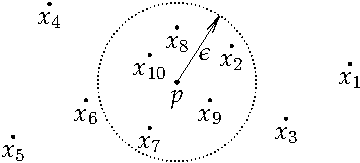
\includegraphics{figures/sequence-convergence-metric}
\caption{Sequence converging to $p$.  The first 10 points 
are shown and $M=7$ for this $\epsilon$.\label{fig:sequence-convergence-metric}}
\end{myfig}
\end{defn}

Let us prove that the limit is unique.  

\begin{prop} \label{prop:mslimisunique}
A convergent sequence in a metric space has a unique limit.
\end{prop}

\begin{proof}
%NOTE: should be word for word the same as 2.1.6
Suppose the sequence $\{ x_n \}$ has limits $x$ and $y$.
Take an arbitrary $\epsilon > 0$.
From the definition find an $n$ such that 
$d(x_n,x) < \nicefrac{\epsilon}{2}$ and
$d(x_n,y) < \nicefrac{\epsilon}{2}$.  Then
\begin{equation*}
d(y,x)
\leq
d(y,x_n) + d(x_n,x)
<
\frac{\epsilon}{2} + \frac{\epsilon}{2} = \epsilon .
\end{equation*}
So $x=y$ and the limit (if it exists) is unique.
\end{proof}

The proofs of the following propositions are left as exercises.

\begin{prop} \label{prop:msconvbound}
A convergent sequence in a metric space is bounded.
\end{prop}

\begin{prop} \label{prop:msconvifa}
A sequence $\{ x_n \}$ in a metric space $(X,d)$ converges to $p \in X$
if and only
if there exists a sequence $\{ a_n \}$ of real numbers such that
\begin{equation*}
d(x_n,p) \leq a_n \quad \text{for all } n \in \N,
\qquad \text{and} \qquad
\lim_{n\to\infty} a_n = 0.
\end{equation*}
\end{prop}

\begin{prop} \label{prop:mssubseq}
Let $\{ x_n \}$ be a sequence in a metric space $(X,d)$.
\begin{enumerate}[(i)]
\item If $\{ x_n \}$ converges to $p \in X$, then every subsequence $\{ x_{n_k} \}$
converges to $p$.
\item If for some $K \in \N$ the $K$-tail $\{ x_n \}_{n=K+1}^\infty$
converges to $p \in X$, then
 $\{ x_n \}$ converges to $p$.
\end{enumerate}
\end{prop}

\begin{exbox}
\begin{exercise}
Prove \propref{prop:msconvbound}.
\end{exercise}

\begin{exercise}
Prove \propref{prop:msconvifa}.
\end{exercise}

\begin{exercise}
Prove \propref{prop:mssubseq}.
\end{exercise}
\end{exbox}

\begin{example}
Take $C([0,1],\R)$ be the set of continuous functions with the metric being
the uniform metric.  We saw that we obtain a metric space.
If we look at the definition of convergence, we notice that it is identical
to uniform convergence.  That is, $\{ f_n \}$ converges uniformly if and only
if it converges in the metric space sense.
\end{example}

\begin{remark}
It is perhaps surprising that on the set of functions $f \colon [a,b] \to
\R$ (continuous or not)
there is no metric that gives pointwise convergence.  Although the proof of
this fact is beyond the scope of this book.
\end{remark}

\begin{exbox}
\begin{exercise}
\begin{exparts}
\item
Show that $d(x,y) = \min \{ 1, \abs{x-y} \}$ defines a metric on $\R$.
\item
Show that a sequence converges in $(\R,d)$ if and only if it converges
in the standard metric.
\item
Find a bounded sequence in $(\R,d)$ that
contains no convergent subsequence.
\end{exparts}
\end{exercise}

\begin{exercise}
Suppose $\{x_n\}_{n=1}^\infty$ converges to $x$.  Suppose $f \colon \N
\to \N$ is a one-to-one function.  Show that
$\{ x_{f(n)} \}_{n=1}^\infty$ converges to $x$.
\end{exercise}

\begin{exercise}
If $(X,d)$ is a metric space where $d$ is the discrete metric.  Suppose 
$\{ x_n \}$ is a convergent sequence in $X$.  Show that there exists
a $K \in \N$ such that for all $n \geq K$ we have $x_n = x_K$.
\end{exercise}

\begin{exercise}
A set $S \subset X$ is said to be \emph{dense} in $X$ if
$X \subset \widebar{S}$ or in other words if for every $x \in X$,
there exists a sequence $\{ x_n \}$ in $S$ that converges to $x$.  Prove
that $\R^n$ contains a countable dense subset.
\end{exercise}

\begin{exercise} \label{exercise:extendedrealsmetric}
Take $\R^* = \{ -\infty \} \cup \R \cup \{ \infty \}$ be the extended reals.
Define $d(x,y) = \bigl\lvert \frac{x}{1+\abs{x}} - \frac{y}{1+\abs{y}}
\bigr\rvert$
if $x, y \in \R$,
define $d(\infty,x) = \bigl\lvert 1 - \frac{x}{1+\abs{x}} \bigr\rvert$,
$d(-\infty,x) = \bigl\lvert 1 + \frac{x}{1+\abs{x}} \bigr\rvert$
for all $x \in \R$, and
let $d(\infty,-\infty) = 2$.
\begin{exparts}
\item
Show that $(\R^*,d)$ is a metric space.
\item
Suppose $\{ x_n \}$ is a sequence of real numbers such that
for every $M \in \R$, there exists an $N$ such that
$x_n \geq M$ for all $n \geq N$.  Show that $\lim\, x_n = \infty$ in
$(\R^*,d)$.
\item
Show that a sequence of real numbers converges to a real number
in $(\R^*,d)$ if and
only if it converges in $\R$ with the standard metric.
\end{exparts}
\end{exercise}

\begin{exercise}
Let $(X,d)$ be a metric space and $\{ x_n \}$ a sequence in $X$.
Prove that $\{ x_n \}$ converges to $p \in X$
if and only if
every subsequence of $\{ x_n \}$ has a subsequence that
converges to $p$.
\end{exercise}
\end{exbox}

\subsection{Convergence in euclidean space}

In $\R^n$, a sequence converges if and only if every
component converges:

\begin{prop} \label{prop:msconveuc}
Let $\{ x_j \}_{j=1}^\infty$ be a sequence in $\R^n$,
where $x_j = \bigl(x_{j,1},x_{j,2},\ldots,x_{j,n}\bigr) \in \R^n$.
Then $\{ x_j \}_{j=1}^\infty$ converges if and only if
$\{ x_{j,k} \}_{j=1}^\infty$ converges for every $k=1,2,\ldots,n$, in which case
\begin{equation*}
\lim_{j\to\infty}
x_j =
\Bigl(
\lim_{j\to\infty} x_{j,1},
\lim_{j\to\infty} x_{j,2},
\ldots,
\lim_{j\to\infty} x_{j,n}
\Bigr) .
\end{equation*}
\end{prop}

\begin{proof}
Suppose
the sequence
$\{ x_j \}_{j=1}^\infty$ converges to
$y = (y_1,y_2,\ldots,y_n) \in \R^n$.
Given $\epsilon > 0$, there exists an $M$, such that for all
$j \geq M$ we have
\begin{equation*}
d(y,x_j) < \epsilon.
\end{equation*}
Fix some $k=1,2,\ldots,n$.  For $j \geq M$ we have
\begin{equation*}
\bigl\lvert y_k - x_{j,k} \bigr\rvert
=
\sqrt{{\bigl(y_k - x_{j,k} \bigr)}^2}
\leq
\sqrt{\sum_{\ell=1}^n {\bigl(y_\ell-x_{j,\ell}\bigr)}^2}
= d(y,x_j) < \epsilon .
\end{equation*}
Hence the sequence $\{ x_{j,k} \}_{j=1}^\infty$ converges to $y_k$.

For the other direction, suppose 
$\{ x_{j,k} \}_{j=1}^\infty$ converges to $y_k$ for every $k=1,2,\ldots,n$.
Given $\epsilon > 0$, pick an $M$, such that if $j \geq M$ then 
$\bigl\lvert y_k-x_{j,k} \bigr\rvert < \nicefrac{\epsilon}{\sqrt{n}}$ for all
$k=1,2,\ldots,n$.  Then
\begin{equation*}
d(y,x_j)
=
\sqrt{\sum_{k=1}^n {\bigl(y_k-x_{j,k}\bigr)}^2}
<
\sqrt{\sum_{k=1}^n {\left(\frac{\epsilon}{\sqrt{n}}\right)}^2}
=
\sqrt{\sum_{k=1}^n \frac{{\epsilon^2}}{n}}
= \epsilon .
\end{equation*}
That is, the sequence $\{ x_j \}$ converges to
$y = (y_1,y_2,\ldots,y_n) \in \R^n$.
\end{proof}

\begin{example}
The set $\C$ of complex numbers $z = x+iy$ is considered 
as the metric space $\R^2$.  The proposition says that the
sequence $\{ z_j \}_{j=1}^\infty = \{ x_j + iy_j \}_{j=1}^\infty$ converges
to $z = x+iy$
if and only if $\{ x_j \}$ converges to $x$ and 
$\{ y_j \}$ converges to $y$.
\end{example}

\begin{exbox}
\begin{exercise}
Consider $\R^n$, and let $d$ be the standard euclidean metric.
Let $d'(x,y) = \sum_{\ell=1}^n \abs{x_\ell-y_\ell}$
and $d''(x,y) = \max \{ \abs{x_1-y_1},\abs{x_2-y_2},\cdots,\abs{x_n-y_n}
\}$.
\begin{exparts}
\item
Use \exerciseref{exercise:mscross}, to show that
$(\R^n,d')$ and
$(\R^n,d'')$ are metric spaces.
\item
Let $\{ x_j \}_{j=1}^\infty$ be a sequence in $\R^n$ and $p \in \R^n$.
Prove that the following statements are equivalent:
\begin{exnumparts}
\item
$\{ x_j \}$ converges to $p$ in $(\R^n,d)$.
\item
$\{ x_j \}$ converges to $p$ in $(\R^n,d')$.
\item
$\{ x_j \}$ converges to $p$ in $(\R^n,d'')$.
\end{exnumparts}
\end{exparts}
\end{exercise}
\end{exbox}

\subsection{Convergence and topology}

The topology, that is, the set of open sets of a space encodes which
sequences converge.

\begin{prop} \label{prop:msconvtopo}
Let $(X,d)$ be a metric space and $\{x_n\}$ a sequence in $X$.  Then
$\{ x_n \}$ converges to $x \in X$ if and only if for every open neighborhood
$U$ of $x$, there exists an $M \in \N$ such that for all $n \geq M$
we have $x_n \in U$.
\end{prop}

\begin{proof}
First suppose $\{ x_n \}$ converges.  Let $U$ be an open neighborhood
of $x$, then there exists an $\epsilon > 0$ such that $B(x,\epsilon) \subset
U$.  As the sequence converges, find an $M \in \N$ such that for all $n \geq
M$ we have $d(x,x_n) < \epsilon$ or in other words $x_n \in B(x,\epsilon)
\subset U$.

Let us prove the other direction.  Given $\epsilon > 0$ let $U =
B(x,\epsilon)$ be the neighborhood of $x$.  Then there is an $M \in \N$
such that for $n \geq M$ we have $x_n \in U = B(x,\epsilon)$ or in other
words, $d(x,x_n) < \epsilon$.
\end{proof}

A set is closed when it contains the limits of its convergent sequences.

\begin{prop} \label{prop:msclosedlim}
Let $(X,d)$ be a metric space, $E \subset X$ a closed set,
and $\{ x_n \}$ a sequence in $E$ that converges to some $x \in X$.
Then $x \in E$.
\end{prop}

\begin{proof}
Let us prove the contrapositive.
Suppose $\{ x_n \}$ is a sequence in $X$ that converges to $x \in E^c$.
As $E^c$ is open, \propref{prop:msconvtopo} says that there is
an $M$ such that for all $n \geq M$,
$x_n \in E^c$.  So $\{ x_n \}$  is not a sequence in $E$.
\end{proof}

To take a closure of a set $A$, we take $A$, and we throw in 
points that are limits of sequences in $A$.

\begin{prop} \label{prop:msclosureapprseq}
Let $(X,d)$ be a metric space and $A \subset X$.
Then $x \in \widebar{A}$ if and only if there exists a sequence $\{ x_n \}$ of
elements in $A$ such that $\lim\, x_n = x$.
\end{prop}

\begin{proof}
Let $x \in \widebar{A}$.  For every $n \in \N$,
by
\propref{prop:msclosureappr} there
exists a point $x_n \in B(x,\nicefrac{1}{n}) \cap A$.
As $d(x,x_n) < \nicefrac{1}{n}$, we have $\lim\, x_n = x$.

For the other direction, see \exerciseref{exercise:reverseclosedseq}.
\end{proof}

\begin{exbox}
\begin{exercise} \label{exercise:reverseclosedseq}
Finish the proof of 
\propref{prop:msclosureapprseq}.
Let $(X,d)$ be a metric space and
let $A \subset X$.  Let $E$ be the set of all $x \in X$ such that there
exists a sequence $\{ x_n \}$ in $A$ that converges to $x$.  Show 
$E = \widebar{A}$.
\end{exercise}

\begin{exercise}
Suppose $\{ U_n \}_{n=1}^\infty$ be a decreasing ($U_{n+1} \subset U_n$ for
all $n$) sequence of open sets in a metric space $(X,d)$ such that
$\bigcap_{n=1}^\infty U_n = \{ p \}$ for some $p \in X$.  Suppose 
$\{ x_n \}$ is a sequence of points in $X$ such that $x_n \in U_n$.  Does
$\{ x_n \}$ necessarily converge to $p$?  Prove or construct a counterexample.
\end{exercise}

\begin{exercise}
Let $E \subset X$ be closed and
let $\{ x_n \}$ be a sequence in $X$ converging to $p \in X$.  Suppose
$x_n \in E$ for infinitely many $n \in \N$.  Show $p \in E$.
\end{exercise}

\begin{exercise}
Suppose $\{ V_n \}_{n=1}^\infty$ is a collection of open sets
in $(X,d)$
such that $V_{n+1} \supset V_n$.  Let $\{ x_n \}$ be a sequence
such that $x_n \in V_{n+1} \setminus V_n$ and suppose 
$\{ x_n \}$ converges to $p \in X$.  Show that $p \in \partial V$
where $V = \bigcup_{n=1}^\infty V_n$.
\end{exercise}
\end{exbox}

%%%%%%%%%%%%%%%%%%%%%%%%%%%%%%%%%%%%%%%%%%%%%%%%%%%%%%%%%%%%%%%%%%%%%%%%%%%%%%

\section{Completeness and compactness}
\label{sec:metcompact}

\subsection{Cauchy sequences and completeness}

Just like with sequences of real numbers we define Cauchy sequences.

\begin{defn}
Let $(X,d)$ be a metric space.
A sequence $\{ x_n \}$ in $X$ is a \emph{\myindex{Cauchy sequence}} if
for every $\epsilon > 0$ there exists an $M \in \N$ such that
for all $n \geq M$ and all $k \geq M$ we have
\begin{equation*}
d(x_n, x_k) < \epsilon .
\end{equation*}
\end{defn}

The definition is again simply a translation of the concept
from the real numbers to metric spaces,
provided we equip the real numbers with
the standard metric $d(x,y) = \abs{x-y}$.

\begin{prop}
A convergent sequence in a metric space is Cauchy.
\end{prop}

\begin{proof}
Suppose $\{ x_n \}$ converges to $x$.
Given $\epsilon > 0$ there is an $M$ such that for $n \geq M$
we have $d(x,x_n) < \nicefrac{\epsilon}{2}$.  Hence
for all $n,k \geq M$ we have
$d(x_n,x_k) \leq d(x_n,x) + d(x,x_k) < \nicefrac{\epsilon}{2} +
\nicefrac{\epsilon}{2} = \epsilon$.
\end{proof}

\begin{defn}
Let $(X,d)$ be a metric space.  We say $X$ is
\emph{\myindex{complete}} or \emph{\myindex{Cauchy-complete}}
if every Cauchy sequence $\{ x_n \}$ in $X$
converges to an $x \in X$.
\end{defn}

\begin{prop}
The space $\R^n$ with the standard metric is a complete metric space.
\end{prop}

We assume the reader has seen the proof of completeness in $\R = \R^1$,
and we reduce the completeness in $\R^n$ to the one dimensional case.

\begin{proof}
Let $\{ x_j \}_{j=1}^\infty$ be a Cauchy sequence
in $\R^n$, where $x_j = \bigl(x_{j,1},x_{j,2},\ldots,x_{j,n}\bigr) \in \R^n$.
Given $\epsilon > 0$, there exists an $M$ such that
$d(x_i,x_j) < \epsilon$
for all
$i,j \geq M$.

Fix some $k=1,2,\ldots,n$, for $i,j \geq M$ we have
\begin{equation*}
\bigl\lvert x_{i,k} - x_{j,k} \bigr\rvert
=
\sqrt{{\bigl(x_{i,k} - x_{j,k}\bigr)}^2}
\leq
\sqrt{\sum_{\ell=1}^n {\bigl(x_{i,\ell}-x_{j,\ell}\bigr)}^2}
= d(x_i,x_j) < \epsilon .
\end{equation*}
Hence the sequence $\{ x_{j,k} \}_{j=1}^\infty$ is Cauchy.  As $\R$ is
complete the sequence converges; there exists an $y_k \in \R$ such that
$y_k = \lim_{j\to\infty} x_{j,k}$.
Write $y = (y_1,y_2,\ldots,y_n) \in \R^n$.
By \propref{prop:msconveuc}, $\{ x_j \}$ converges
to $y \in \R^n$ and hence $\R^n$ is complete.
\end{proof}

A subset of $\R^n$ with the subspace metric need not be
complete.  For example, $(0,1]$ with the subspace metric is not
complete as $\{ \nicefrac{1}{n} \}$ is a Cauchy sequence in $(0,1]$
with no limit in $(0,1]$.  But see also
\exerciseref{exercise:closedcomplete}.

In the language of metric spaces,
as uniform limits of continuous functions are continuous,
the metric space
$C([a,b],\R)$ of \exampleref{example:msC01} is complete.
The proof follows by ``unrolling the definitions,'' 
and is left as an exercise.

\begin{prop} \label{prop:CabRcomplete}
The space of continuous functions $C([a,b],\R)$ with the uniform
norm as metric is a complete metric space.
\end{prop}

Once we have one complete metric space, any closed subspace is
also a complete metric space.  After all, one way
to think of a closed set is that it contains all points
that can be reached from the set via a sequence.
The proof is again an exercise.

\begin{prop} \label{prop:closedcomplete}
Suppose $(X,d)$ is a complete metric space and $E \subset X$
is closed, then $E$ is a complete metric space with the subspace topology.
\end{prop}

\begin{exbox}
\begin{exercise} \label{exercise:closedcomplete}
Prove \propref{prop:closedcomplete}.  That is,
let $(X,d)$ be a complete metric space and $E \subset X$ a closed set.
Show that $E$ with the subspace metric is a complete metric space.
\end{exercise}

\begin{exercise} \label{exercise:CabRcomplete}
Let $C([a,b],\R)$ be the metric space as in \exampleref{example:msC01}.  Show that
$C([a,b],\R)$ is a complete metric space.
\end{exercise}
\end{exbox}

\subsection{Compactness}

\begin{defn}
Let $(X,d)$ be a metric space and $K \subset X$. 
The set $K$ is said to be \emph{\myindex{compact}}
if for any collection
of open sets $\{ U_{\lambda} \}_{\lambda \in I}$ such that
\begin{equation*}
K \subset \bigcup_{\lambda \in I} U_\lambda ,
\end{equation*}
there exists a finite subset
$\{ \lambda_1, \lambda_2,\ldots,\lambda_k \} \subset I$
such that
\begin{equation*}
K \subset \bigcup_{j=1}^k U_{\lambda_j} .
\end{equation*}
\end{defn}

A collection of open sets $\{ U_{\lambda} \}_{\lambda \in I}$ as above is
said to be an \emph{\myindex{open cover}} of $K$.  So a way to say that
$K$ is compact is to say that \emph{every open cover of $K$ has a finite
\myindex{subcover}}.

\begin{example}
Let $\R$ be the metric space with the standard metric.

The set $\R$ is not compact.  Proof: Take the sets $U_j = (-j,j)$.
Any $x \in \R$ is in some $U_j$, so we have an open cover.
Suppose we have a finite
subcover $\R \subset U_{j_1} \cup U_{j_2} \cup \cdots \cup U_{j_k}$,
and suppose $j_1 < j_2 < \cdots < j_k$.  Then $\R \subset U_{j_k}$, but that is
a contradiction as $j_k \in \R$ on one hand and $j_k \notin U_{j_k} =
(-j_k,j_k)$ on the
other.

The set $(0,1) \subset \R$ is also not compact.  Proof:  Take the 
sets $U_{j} = (\nicefrac{1}{j},1-\nicefrac{1}{j})$ for $j=3,4,5,\ldots$.
As above $(0,1) = \bigcup_{j=3}^\infty U_j$.  And similarly as above,
if there exists a finite subcover, then there is one $U_j$ such that $(0,1)
\subset U_j$, which again leads to a contradiction.

The set $\{ 0 \} \subset \R$ is compact.  Proof: Given any open cover $\{
U_{\lambda} \}_{\lambda \in I}$, there must exist a $\lambda_0$ such that $0
\in U_{\lambda_0}$ as it is a cover.  But then $U_{\lambda_0}$ gives a
finite subcover.

We will prove below that $[0,1]$, and in fact any closed and bounded
interval $[a,b]$ is compact.
\end{example}

\begin{prop}
Let $(X,d)$ be a metric space.  A compact set $K \subset X$ is closed and
bounded.
\end{prop}

\begin{proof}
Let $K$ be a compact set.
Fix $p \in X$.  We have the open cover
\begin{equation*}
K \subset \bigcup_{n=1}^\infty B(p,n) = X .
\end{equation*}
If $K$ is compact, then there exists some set of indices
$n_1 < n_2 < \ldots < n_k$ such that
\begin{equation*}
K \subset \bigcup_{j=1}^k B(p,n_j) = B(p,n_k) .
\end{equation*}
So $K$ is bounded.
See left hand side of \figureref{fig:compactbndclosed}.

Next, we show a set that is not closed is not compact.  Suppose 
$\widebar{K} \not= K$, that is, there is a point $x \in \widebar{K}
\setminus K$.
We have the open cover
%If $y \not= x$, then
%$y \notin C(x,\nicefrac{1}{n})$
%for $n \in \N$
%such that $\nicefrac{1}{n} < d(x,y)$.
%Furthermore $x \notin K$, so
\begin{equation*}
K \subset \bigcup_{n=1}^\infty {C(x,\nicefrac{1}{n})}^c .
\end{equation*}
%A closed ball is closed, so its complement ${C(x,\nicefrac{1}{n})}^c$ is open, and
%we have an open cover.
If we take any
finite collection of indices $n_1 < n_2 < \ldots < n_k$, then 
\begin{equation*}
\bigcup_{j=1}^k {C(x,\nicefrac{1}{n_j})}^c 
=
{C(x,\nicefrac{1}{n_k})}^c 
\end{equation*}
As $x$ is in the closure of $K$,
then
$C(x,\nicefrac{1}{n_k}) \cap K \not= \emptyset$.  So there is no
finite subcover and $K$ is not compact.
See right hand side of \figureref{fig:compactbndclosed}.
\end{proof}

\begin{myfig}
\subimport*{figures/}{compactbnd.pdf_t}
\qquad \qquad
\subimport*{figures/}{compactclosed.pdf_t}
\caption{Proving compact set is bounded (left) and closed (right).\label{fig:compactbndclosed}}
\end{myfig}

We prove below that 
in finite dimensional euclidean space
every closed bounded set is compact.
So closed bounded sets
of $\R^n$ are examples of compact sets.
It is not true that in every metric space, closed and bounded is equivalent
to compact.  A simple example is an incomplete metric space such as
$(0,1)$ with the subspace metric from $\R$.
There are many complete and very useful metric spaces
where closed and bounded is not
enough to give compactness: $C([a,b],\R)$ is a complete metric
space, but the closed unit ball $C(0,1)$ is not compact, see
\exerciseref{exercise:msclbounnotcompt}.  However, see also
\exerciseref{exercise:mstotbound}.

A useful property of compact sets in a metric space is that every
sequence in the set has a convergent subsequence converging
to a point in the set.
Such sets are called
\emph{\myindex{sequentially compact}}.
Let us prove that in the
context of metric spaces, a set is compact if and only if it is sequentially
compact.
First we prove a lemma.

\begin{lemma}[Lebesgue covering lemma%
\footnote{The number $\delta$ is sometimes called the
\myindex{Lebesgue number} of the cover.}]\label{ms:lebesgue}
\index{Lebesgue covering lemma}
Let $(X,d)$ be a metric space and $K \subset X$.  Suppose 
every sequence in $K$ has a subsequence convergent in $K$.  Given
an open cover $\{ U_\lambda \}_{\lambda \in I}$ of $K$, there exists a
$\delta > 0$ such that for every $x \in K$, there exists a $\lambda \in I$
with $B(x,\delta) \subset U_\lambda$.
\end{lemma}

\begin{proof}
We prove the lemma by contrapositive.
If the conclusion is not true, then
there is
an open cover $\{ U_\lambda \}_{\lambda \in I}$ of $K$ with
the following property.
For every $n \in \N$ there exists an $x_n \in K$ such that
$B(x_n,\nicefrac{1}{n})$ is not a subset of any $U_\lambda$.
Take any $x \in K$.  There is
a $\lambda \in I$ such that $x \in U_\lambda$.  As $U_\lambda$ is open,
there is an $\epsilon > 0$ 
such that $B(x,\epsilon) \subset U_\lambda$.  Take $M$ such that
$\nicefrac{1}{M} < \nicefrac{\epsilon}{2}$.  If $y \in 
B(x,\nicefrac{\epsilon}{2})$ and $n \geq M$, then 
\begin{equation*}
B(y,\nicefrac{1}{n}) \subset
B(y,\nicefrac{1}{M}) \subset
B(y,\nicefrac{\epsilon}{2}) \subset B(x,\epsilon)
\subset U_\lambda ,
\end{equation*}
where 
$B(y,\nicefrac{\epsilon}{2}) \subset B(x,\epsilon)$
follows by triangle inequality.
See \figureref{fig:lebesguedelta}.
In other words, for all $n \geq M$, $x_n \notin B(x,\nicefrac{\epsilon}{2})$. 
The sequence cannot have a subsequence converging to $x$.  As $x \in K$ was
arbitrary we are done.
\end{proof}

\begin{myfig}
\subimport*{figures/}{lebesguedelta.pdf_t}
\caption{Proof of Lebesgue covering lemma.
Note that $B(y,\nicefrac{\epsilon}{2}) \subset
B(x,\epsilon)$ by triangle inequality.\label{fig:lebesguedelta}}
\end{myfig}

It is important to recognize what the lemma says.  It says that
if $K$ is sequentially compact, then given any
cover there is a single $\delta > 0$.  The $\delta$ depends on the cover,
but of course it does not depend on $x$.

For example, let $K = [-10,10]$ and for $n \in \Z$ let $U_n =
(n,n+2)$ define sets in an open cover.
Take $x \in K$. There is an $n \in \Z$, 
such that $n \leq x < n+1$.
If $n \leq x < n+\nicefrac{1}{2}$, then
$B\bigl(x,\nicefrac{1}{2}\bigr) \subset U_{n-1}$.
If $n+ \nicefrac{1}{2} \leq x < n+1$, then
$B\bigl(x,\nicefrac{1}{2}\bigr) \subset U_{n}$.  So $\delta =
\nicefrac{1}{2}$.  If instead we let $U'_n =
\bigl(\frac{n}{2},\frac{n+2}{2} \bigr)$, then we again obtain an open
cover, but now the best $\delta$ we can find is $\nicefrac{1}{4}$.

%On the other hand, $\N \subset \R$ is not sequentially compact.
%It is an exercise to find a cover for which no $\delta > 0$ works.


\begin{thm} \label{thm:mscompactisseqcpt}
Let $(X,d)$ be a metric space.  Then $K \subset X$ is compact if
and only if every sequence in $K$ has a subsequence converging to
a point in $K$.
\end{thm}

\begin{proof}
Claim: \emph{Let $K \subset X$ be a subset of $X$ and
$\{ x_n \}$ a sequence in $K$.  Suppose that for each $x \in K$,
there is a ball $B(x,\alpha_x)$ for some $\alpha_x > 0$ such that
$x_n \in B(x,\alpha_x)$ for only finitely many $n \in \N$.
Then $K$ is not compact.}

Proof of the claim:
Notice
\begin{equation*}
K \subset \bigcup_{x \in K} B(x,\alpha_x) .
\end{equation*}
Any finite collection of these balls is going to contain only finitely many
$x_n$.  Thus for any finite collection of such balls there is an $x_n \in K$
that is not in the union.  Therefore, $K$ is not compact and the claim is
proved.

So suppose that $K$ is compact and $\{ x_n \}$ is a sequence in $K$.
Then there exists an $x \in K$ such that
for any $\delta > 0$,
$B(x,\delta)$ contains $x_k$ for infinitely many $k \in \N$.
We define the subsequence inductively.
The ball $B(x,1)$ contains some $x_k$ so let $n_1 = k$.
Suppose $n_{j-1}$ is defined.
There must exist a $k > n_{j-1}$
such that $x_k \in B(x,\nicefrac{1}{j})$.  So define
$n_j = k$.
We now posses a subsequence $\{ x_{n_j} \}_{j=1}^\infty$.
Since
$d(x,x_{n_j}) < \nicefrac{1}{j}$,  \propref{prop:msconvifa} says
$\lim\, x_{n_j} = x$.

For the other direction, suppose every sequence in $K$
has a 
subsequence converging in $K$.
Take
an open cover $\{ U_\lambda \}_{\lambda \in I}$ of $K$.
Using the Lebesgue covering lemma above, find a $\delta > 0$
such that for every $x \in K$, there is a $\lambda \in I$ with
$B(x,\delta) \subset U_\lambda$.

Pick $x_1 \in K$ and find $\lambda_1 \in I$ such that $B(x_1,\delta) \subset
U_{\lambda_1}$.
If $K \subset U_{\lambda_1}$, we stop as we have found a
finite subcover.
Otherwise, there must be
a point $x_2 \in K \setminus U_{\lambda_1}$.
Note that $d(x_2,x_1) \geq \delta$.
There must exist some $\lambda_2 \in I$ such that
$B(x_2,\delta) \subset U_{\lambda_2}$.
We work inductively.  Suppose $\lambda_{n-1}$ is defined.
Either
$U_{\lambda_1} \cup
U_{\lambda_2} \cup \cdots \cup
U_{\lambda_{n-1}}$ is a finite cover of $K$, in which case we
stop, or
there must be 
a point $x_n \in K \setminus \bigl( U_{\lambda_1} \cup
U_{\lambda_2} \cup \cdots \cup
U_{\lambda_{n-1}}\bigr)$.
Note that $d(x_n,x_j) \geq \delta$ for all $j = 1,2,\ldots,n-1$.
Next, there must be some $\lambda_n \in I$
such that $B(x_n,\delta) \subset U_{\lambda_n}$.
See \figureref{fig:seqcompactiscompact}.

\begin{myfig}
\subimport*{figures/}{seqcompactiscompact.pdf_t}
\caption{Covering $K$ by $U_{\lambda}$.  The points
$x_1,x_2,x_3,x_4$, 
the three sets 
$U_{\lambda_1}$,
$U_{\lambda_2}$,
$U_{\lambda_2}$,
and 
the first three balls
of radius $\delta$ are drawn.\label{fig:seqcompactiscompact}}
\end{myfig}

Either at some point we obtain a finite subcover of $K$,
or we obtain an
infinite
sequence $\{ x_n \}$ as above.
For contradiction, suppose that
there is no finite subcover and we have the sequence $\{ x_n \}$.
For all $n$ and $k$, $n \not= k$, 
we have $d(x_n,x_k) \geq \delta$,
so no subsequence of $\{ x_n \}$ can be
Cauchy.  Hence no subsequence of $\{ x_n \}$ can be convergent,
which is a contradiction.
\end{proof}

\begin{example}
The Bolzano--Weierstrass theorem for sequences of real numbers
says that any bounded sequence in $\R$ has a convergent
subsequence.  Therefore, any sequence in a closed interval $[a,b] \subset \R$ has 
a convergent subsequence.  The limit must also be in $[a,b]$ as limits
preserve non-strict inequalities.  Hence a closed bounded interval $[a,b]
\subset \R$ is compact.
\end{example}

\begin{prop}
Let $(X,d)$ be a metric space and let $K \subset X$ be compact.  If
$E \subset K$ is a closed set, then $E$ is compact.
\end{prop}

Because $K$ is closed then $E$ is closed in $K$ if
and only if it is closed in $X$,
see \propref{prop:topology:subspacesame}.

\begin{proof}
Let $\{ x_n \}$ be a sequence in $E$.  It is also a sequence in $K$.
Therefore, it has a convergent subsequence $\{ x_{n_j} \}$ that converges to
some $x \in K$.  As $E$ is closed the limit of a sequence in $E$ is also in $E$
and so $x \in E$.  Thus $E$ must be compact.
\end{proof}

\begin{thm}[Heine--Borel] \index{Heine--Borel theorem}
\label{thm:msbw}
A closed bounded subset $K \subset \R^n$ is compact.
\end{thm}

So subsets of $\R^n$ are compact if and only if they are closed and bounded,
a condition that is much easier to check.
Let us reiterate that the Heine--Borel theorem only holds for $\R^n$ and not
for metric spaces in general.  In general, compact implies closed and
bounded, but not vice-versa.

\begin{proof}
For $\R = \R^1$ if $K \subset \R$ is closed and bounded, then
any sequence $\{ x_k \}$ in $K$ is bounded, so it has a convergent
subsequence by
the Bolzano--Weierstrass theorem.
As $K$ is closed, the limit of the subsequence must be an element of
$K$.  So $K$ is compact.

Let us carry out the proof for $n=2$ and leave arbitrary $n$ as an exercise.
As $K \subset \R^2$ is bounded, there exists a set
$B=[a,b]\times[c,d] \subset \R^2$ such that $K \subset B$.  We will show
that $B$ is compact.  Then $K$, being a closed subset of a compact $B$, is
also compact.  

Let $\bigl\{ (x_k,y_k) \bigr\}_{k=1}^\infty$ be a sequence in $B$.  That is,
$a \leq x_k \leq b$ and
$c \leq y_k \leq d$ for all $k$.  A bounded sequence of real numbers
has a convergent
subsequence so there is a subsequence $\{ x_{k_j} \}_{j=1}^\infty$
that is convergent.  The subsequence 
$\{ y_{k_j} \}_{j=1}^\infty$ is also a bounded sequence so there exists
a subsequence
$\{ y_{k_{j_i}} \}_{i=1}^\infty$ that is convergent.  A subsequence of a
convergent sequence is still convergent, so 
$\{ x_{k_{j_i}} \}_{i=1}^\infty$ is convergent.
Let
\begin{equation*}
x = \lim_{i\to\infty} x_{k_{j_i}}
\qquad \text{and} \qquad
y = \lim_{i\to\infty} y_{k_{j_i}} .
\end{equation*}
By \propref{prop:msconveuc},
$\bigl\{ (x_{k_{j_i}},y_{k_{j_i}}) \bigr\}_{i=1}^\infty$ converges to $(x,y)$.
Furthermore, as $a \leq x_k \leq b$ and
$c \leq y_k \leq d$ for all $k$, we know that $(x,y) \in B$.
\end{proof}

\begin{exbox}
\begin{exercise}
Prove \thmref{thm:msbw} for arbitrary dimension.
Hint: The trick is to use the correct notation.
\end{exercise}
\end{exbox}

\begin{prop}
Suppose $(X,d)$ is a metric space
and $E_1$, $E_2$, \ldots, are
nonempty compact subsets of $X$ such that
$E_1 \supset E_2 \supset E_3 \supset \cdots$.  Then
\begin{equation*}
\bigcap_{j=1}^\infty E_j \not= \emptyset .
\end{equation*}
\end{prop}

\begin{proof}
Compact sets are closed so their complement is open.  Consider
$U_k = X \setminus E_k$.  If the intersection would be empty,
then $\{ U_k \}$ would be an open cover of $E_1$, which is compact,
and hence there would be a finite subcover, in particular
as $U_k \subset U_{k+1}$, $E_1 \subset U_k$ for some $k$, which would imply
that $E_k$ is empty.
\end{proof}

\begin{example}
The discrete metric provides interesting counterexamples again.
Let $(X,d)$ be a metric space with the discrete metric, that is $d(x,y) = 1$
if $x \not= y$.  Suppose
$X$ is an infinite set.  Then:
\begin{enumerate}[(i)]
\item $(X,d)$ is a complete metric space.
\item Any subset $K \subset X$ is closed and bounded.
\item A subset $K \subset X$ is compact if and only if it is a finite set.
\item The conclusion of the Lebesgue covering lemma is always satisfied with
e.g. $\delta = \nicefrac{1}{2}$, even for noncompact $K \subset X$.
\end{enumerate}
The proofs
of the statements above are either trivial or are relegated to the exercises
below.
\end{example}

\begin{remark}
A subtle issue with Cauchy sequences, completeness, compactness,
and convergence is that compactness and convergence only depend on the
topology, that is, on which sets are the open sets.  On the other hand,
Cauchy sequences and completeness depend on the actual metric.
\end{remark}

\begin{exbox}
\begin{exercise}
Let $(X,d)$ be a metric space and $A$ a finite subset of $X$.
Show that $A$ is compact.
\end{exercise}

\begin{exercise}
Let $A = \{ \nicefrac{1}{n} : n \in \N \} \subset \R$.
\begin{exparts}
\item
Show that $A$ is
not compact directly using the definition.
\item
Show that $A \cup \{ 0 \}$ is
compact directly using the definition.
\end{exparts}
\end{exercise}

\begin{exercise}
Let $(X,d)$ be a metric space with the discrete metric.
\begin{exparts}
\item
Prove that $X$ is complete.
\item
Prove that $X$ is compact if and only if $X$ is a finite set.
\end{exparts}
\end{exercise}

\begin{exercise}
\begin{exparts}
\item
Show that the union of finitely many compact sets is a compact set.
\item
Find an example where the union of infinitely many compact sets is not
compact.
\end{exparts}
\end{exercise}

\begin{exercise}
Show that a compact set $K$ is a complete metric space (using the subspace
metric).
\end{exercise}

\begin{exercise} \label{exercise:msclbounnotcompt}
Let $C([0,1],\R)$ be the metric space of \exampleref{example:msC01}.  Let $0$
denote the zero function.  Then show that the closed ball
$C(0,1)$ is not compact (even though it is closed and bounded).
Hints: Construct a sequence of distinct continuous functions $\{ f_n \}$ such that
$d(f_n,0) = 1$ and $d(f_n,f_k) = 1$ for all $n \not= k$.  Show that
the set $\{ f_n : n \in \N \} \subset C(0,1)$ is closed but not compact.
\end{exercise}

%\begin{exercise}[Challenging]
%Show that there exists a metric on $\R$ that makes $\R$ into a compact set.
%\end{exercise}

%\begin{exercise}
%Suppose $(X,d)$ is complete and suppose we have a countably infinite
%collection of nonempty compact sets $E_1 \supset E_2 \supset E_3 \supset
%\cdots$.  Prove $\bigcap_{j=1}^\infty E_j \not= \emptyset$.
%\end{exercise}

\begin{exercise}
Let $C([0,1],\R)$ be the metric space of \exampleref{example:msC01}.
Let $K$ be the set of $f \in C([0,1],\R)$ such that
$f$ is equal to a quadratic polynomial, i.e.\ $f(x) = a+bx+cx^2$, and such that
$\abs{f(x)} \leq 1$ for all $x \in [0,1]$,
that is $f \in C(0,1)$.  Show that $K$ is compact.
\end{exercise}

\begin{exercise} \label{exercise:mstotbound}
Let $(X,d)$ be a complete metric space.
Show that $K \subset X$ is compact if and only if $K$ is closed
and such that for every $\epsilon > 0$
there exists a finite set of points $x_1,x_2,\ldots,x_n$ with
$K \subset \bigcup_{j=1}^n B(x_j,\epsilon)$.
Note: Such a set $K$ is said to be \emph{\myindex{totally bounded}},
so in a complete metric space a set is compact if and only
if it is closed and totally bounded.
\end{exercise}

\begin{exercise}
Take $\N \subset \R$ using the standard metric.  Find an open cover of $\N$
such that the conclusion of the Lebesgue covering lemma does not hold.
\end{exercise}

\begin{exercise}
Prove the general \myindex{Bolzano--Weierstrass theorem}:
Any bounded sequence $\{ x_k
\}$ in $\R^n$ has a convergent subsequence.
\end{exercise}

\begin{exercise}
Let $X$ be a metric space and
$C \subset \sP(X)$ the set of nonempty compact subsets of $X$.
Using the Hausdorff metric from \exerciseref{exercise:mshausdorffpseudo},
show that $(C,d_H)$ is a metric space.  That is, show that
if $L$ and $K$ are nonempty compact subsets then $d_H(L,K) = 0$
if and only if $L=K$.
\end{exercise}

\begin{exercise}
Let $(X,d)$ be an incomplete metric space.  Show that there exists a
closed and bounded set $E \subset X$ that is not compact.
\end{exercise}

\begin{exercise}
Let $(X,d)$ be a metric space and $K \subset X$.
Prove that $K$ is compact as a subset of $(X,d)$ if and only if $K$ is
compact as a subset of itself with the subspace metric.
\end{exercise}

\begin{exercise} \label{exercise:relativelycompactseq}
Let $(X,d)$ be a complete metric space.
We say a set $S \subset X$ is \emph{\myindex{relatively compact}}
if the closure $\widebar{S}$ is compact.
Prove that $S \subset X$ is relatively compact if and only if
given any sequence $\{ x_n \}$ in $S$, there exists a subsequence
$\{ x_{n_k} \}$ that converges (in $X$).
\end{exercise}
\end{exbox}

%%%%%%%%%%%%%%%%%%%%%%%%%%%%%%%%%%%%%%%%%%%%%%%%%%%%%%%%%%%%%%%%%%%%%%%%%%%%%%

\section{Continuous functions}
\label{sec:metcont}

\subsection{Continuity}

\begin{defn}
Let $(X,d_X)$ and $(Y,d_Y)$ be metric spaces and $c \in X$.
Then $f \colon X \to Y$ is
\emph{continuous at $c$}\index{continuous at $c$}
if for every $\epsilon > 0$
there is a $\delta > 0$ such that whenever $x \in X$ and $d_X(x,c) <
\delta$, then
$d_Y\bigl(f(x),f(c)\bigr) < \epsilon$.

\medskip

When $f \colon X \to Y$ is continuous at all $c \in X$, then we simply say
that $f$ is a \emph{continuous function}\index{continuous function!in a
metric space}\index{function!continuous}.
\end{defn}

\begin{prop} \label{prop:contiscont}
Let $(X,d_X)$ and $(Y,d_Y)$ be metric spaces.
Then $f \colon X \to Y$ is
continuous at $c \in X$
if and only if for every sequence $\{ x_n \}$ in $X$
converging to $c$, the sequence $\{ f(x_n) \}$ converges
to $f(c)$.
\end{prop}

\begin{proof}
Suppose $f$ is continuous at $c$.  Let $\{ x_n \}$ be a
sequence in $X$ converging to $c$.  Given $\epsilon > 0$,
there is a $\delta > 0$ such that $d_X(x,c) < \delta$ implies
$d_Y\bigl(f(x),f(c)\bigr) < \epsilon$.  So take $M$ such that
for all $n \geq M$, we have $d_X(x_n,c) < \delta$, then
$d_Y\bigl(f(x_n),f(c)\bigr) < \epsilon$.  Hence $\{ f(x_n) \}$
converges to $f(c)$.

Now suppose $f$ is not continuous at $c$.
Then there exists an $\epsilon > 0$,
such that for every $n \in \N$ there is an $x_n \in X$,
with
$d_X(x_n,c) < \nicefrac{1}{n}$ such that $d_Y\bigl(f(x_n),f(c)\bigr) \geq
\epsilon$.  So $\{ x_n \}$ converges to $c$, but $\{ f(x_n) \}$
does not converge to $f(c)$.
\end{proof}

\begin{example}
Suppose $f \colon \R^2 \to \R$ is a polynomial.  That is,
\begin{equation*}
\begin{split}
f(x,y) & =
\sum_{j=0}^d
\sum_{k=0}^{d-j}
a_{jk}\,x^jy^k \\
& =
a_{0\,0} + a_{1\,0} \, x +
a_{0\,1} \, y+  
a_{2\,0} \, x^2+  
a_{1\,1} \, xy+  
a_{0\,2} \, y^2+ \cdots +
a_{0\,d} \, y^d ,
\end{split}
\end{equation*}
for some $d \in \N$ (the degree) and $a_{jk} \in \R$.  Then we claim 
$f$ is continuous.  Let $\{ (x_n,y_n) \}_{n=1}^\infty$ be a sequence
in $\R^2$ that converges to $(x,y) \in \R^2$.  We proved that this
means $\lim\, x_n = x$ and $\lim\, y_n = y$.  Then
\begin{equation*}
\lim_{n\to\infty}
f(x_n,y_n) =
\lim_{n\to\infty}
\sum_{j=0}^d
\sum_{k=0}^{d-j}
a_{jk} \, x_n^jy_n^k 
=
\sum_{j=0}^d
\sum_{k=0}^{d-j}
a_{jk} \, x^jy^k
=
f(x,y) .
\end{equation*}
So $f$ is continuous at $(x,y)$, and as $(x,y)$ was arbitrary $f$ is
continuous everywhere.  Similarly, a
polynomial in $n$ variables is continuous.
\end{example}

Be careful about taking limits separately.  It is not enough that
for any $y$, the function $g(x) = f(x,y)$ is
continuous, and for and for any $x$, that the function $h(y) = f(x,y)$
is continuous.  The function $f(x,y)$ could still be discontinuous.

\begin{exbox}
\begin{exercise}
Let $f \colon \R^2 \to \R$ be defined by $f(0,0) = 0$, and
$f(x,y) = \frac{xy}{x^2+y^2}$ if $(x,y) \not= (0,0)$.
See \figureref{fig:xyxsqysq}.
\begin{exparts}
\item
Show that for any fixed $x$,
the function that takes $y$ to $f(x,y)$ is continuous.  Similarly
for any fixed $y$, the function that takes $x$ to $f(x,y)$ is continuous.
\item
Show that $f$ is not continuous.
\end{exparts}
\end{exercise}
\end{exbox}

\begin{myfig}
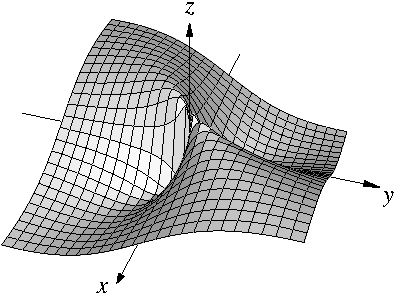
\includegraphics{figures/xyxsqysq}
\caption{Graph of $\frac{xy}{x^2+y^2}$.\label{fig:xyxsqysq}}
\end{myfig}

\begin{example}
Let $X$ be a metric space and $f \colon X \to \C$ a complex-valued
function.  Write $f(p) = g(p) + i h(p)$, where $g \colon X \to \R$
and $h \colon X \to \R$ are the real and imaginary parts of $f$.
Then $f$ is continuous at $c \in X$ if and only if its real
and imaginary parts are continuous at $c$.  
This fact follows because $\{ f(p_n) = g(p_n) + i h(p_n) \}_{n=1}^\infty$
converges to $f(p) = g(p) + i h(p)$ if and only if
$\{ g(p_n) \}$ converges to $g(p)$ and
$\{ h(p_n) \}$ converges to $h(p)$.
\end{example}

\begin{exbox}
\begin{exercise} \label{exercise:continuousintoperator}
Take the metric space of continuous functions $C([0,1],\R)$.  Let
$k \colon [0,1] \times [0,1] \to \R$ be a continuous function.
Given $f \in C([0,1],\R)$ define
\begin{equation*}
\varphi_f(x) = \int_0^1 k(x,y) f(y)  \, dy .
\end{equation*}
\begin{exparts}
\item
Show that $T(f) = \varphi_f$ defines a function $T \colon C([0,1],\R) \to
C([0,1],\R)$.
\item
Show that $T$ is continuous.
\end{exparts}
\end{exercise}

\begin{exercise} \label{exercise:metriccontinuous}
Let $(X,d)$ be a metric space.
\begin{exparts}
\item
If $p \in X$,
show that $f \colon X \to \R$ defined
by $f(x) = d(x,p)$ is continuous.
\item
Define a metric on $X \times X$ as in \exerciseref{exercise:mscross} part
b, and show that $g \colon X \times X \to \R$ defined by
$g(x,y) = d(x,y)$ is continuous.
\end{exparts}
\end{exercise}

\begin{exercise}
Let $C([a,b],\R)$ be the set of continuous functions and
$C^1([a,b],\R)$\glsadd{not:contdifffuncs} the set of once continuously differentiable
functions on $[a,b]$.
Define
\begin{equation*}
d_{C}(f,g) = \snorm{f-g}_S
\qquad \text{and} \qquad
d_{C^1}(f,g) = \snorm{f-g}_S + \snorm{f'-g'}_S,
\end{equation*}
where $\snorm{\cdot}_S$ is the uniform norm.
By \exampleref{example:msC01} and \exerciseref{exercise:C1ab} we know that
$C([a,b],\R)$ with $d_C$ is a metric space and
so is
$C^1([a,b],\R)$ with $d_{C^1}$.
\begin{exparts}
\item
Prove that the derivative operator $D \colon 
C^1([a,b],\R) \to C([a,b],\R)$ defined by
$D(f) = f'$ is continuous.
\item
On the other hand if we consider the metric $d_C$ on $C^1([a,b],\R)$,
then prove the derivative operator is no longer continuous.  Hint: Consider
$\sin(n x)$.
\end{exparts}
\end{exercise}

\begin{exercise}
Define
\begin{equation*}
f(x,y) =
\begin{cases}
\frac{2xy}{x^4+y^2} & \text{if } (x,y) \not= (0,0) \\
0 & \text{if } (x,y) = (0,0) .
\end{cases}
\end{equation*}
\begin{exparts}
\item
Show that for every fixed $y$ the function that takes $x$ to $f(x,y)$
is continuous and hence Riemann integrable.
\item
For every fixed $x$, the function that takes $y$ to $f(x,y)$ is continuous.
\item
Show that $f$ is not continuous at $(0,0)$.
\item
Now show that $g(y) = \int_0^1 f(x,y)\,dx$ is not continuous at $y=0$.
\end{exparts}
Note: Feel free to use what you know about $\arctan$ from calculus,
in particular that $\frac{d}{ds} \bigl[ \arctan(s) \bigr] = \frac{1}{1+s^2}$.
\end{exercise}

\end{exbox}


\subsection{Compactness and continuity}

Continuous maps do not map closed sets to closed sets.  For example,
$f \colon (0,1) \to \R$ defined by $f(x) = x$ takes the set $(0,1)$, which
is closed in $(0,1)$, to the set $(0,1)$, which is not closed in $\R$.
On the other hand continuous maps do preserve compact sets.

\begin{lemma} \label{lemma:continuouscompact}
Let $(X,d_X)$ and $(Y,d_Y)$ be metric spaces
and $f \colon X \to Y$ a continuous function.  If
$K \subset X$ is a compact set, then $f(K)$ is a compact set.
\end{lemma}

\begin{proof}
A sequence in $f(K)$ can be written as
$\{ f(x_n) \}_{n=1}^\infty$, where
$\{ x_n \}_{n=1}^\infty$ is a sequence in $K$.  The set $K$ is compact and
therefore there is a subsequence
$\{ x_{n_j} \}_{j=1}^\infty$ that converges to some $x \in K$.
By continuity,
\begin{equation*}
\lim_{j\to\infty} f(x_{n_j}) = f(x) \in f(K) .
\end{equation*}
So every sequence in $f(K)$ has a subsequence convergent to 
a point in $f(K)$, and $f(K)$ is compact by \thmref{thm:mscompactisseqcpt}.
\end{proof}

As before, $f \colon X \to \R$ achieves an
\emph{\myindex{absolute minimum}} at $c \in X$ if
\begin{equation*}
f(x) \geq f(c) \qquad \text{for all } x \in X.
\end{equation*}
On the other hand, $f$ achieves an 
\emph{\myindex{absolute maximum}} at $c \in X$ if
\begin{equation*}
f(x) \leq f(c) \qquad \text{for all } x \in X.
\end{equation*}

\begin{thm}
Let $(X,d)$ be a compact metric space
and $f \colon X \to \R$ a continuous function.  Then
$f$ achieves an absolute minimum and maximum on $X$.
In particular, $f$ is bounded.
\end{thm}

\begin{proof}
As $X$ is compact and $f$ is continuous, then
$f(X) \subset \R$ is compact.  Hence $f(X)$ is closed
and bounded.  In particular,
$\sup f(X) \in f(X)$ and
$\inf f(X) \in f(X)$, because both the sup and the inf
can be achieved by sequences in $f(X)$ and $f(X)$ is closed.
Therefore, there is some $x \in X$ such that $f(x) = \sup f(X)$
and some $y \in X$ such that $f(y) = \inf f(X)$.
\end{proof}

\begin{exbox}
\begin{exercise}
Let $(X,d)$ be a metric space.
Use \exerciseref{exercise:metriccontinuous} to prove that
if $K_1$ and $K_2$ are compact subsets of $X$, then
there exists a $p \in K_1$ and $q \in K_2$ such that $d(p,q)$ is minimal,
that is, $d(p,q) = \inf \{ d(x,y) \colon x \in K_1, y \in K_2 \}$.
\end{exercise}

\begin{exercise}
Let $(X,d)$ be a compact metric space, let $C(X,\R)$ be the set
of real-valued continuous functions.  Define
\begin{equation*}
d(f,g) = \snorm{f-g}_S = \sup_{x \in X} \abs{f(x)-g(x)} .
\end{equation*}
\begin{exparts}
\item
Show that $d$ makes $C(X,\R)$ into a metric space.
\item
Show that for any $x \in X$, the evaluation function
$E_x \colon C(X,\R) \to \R$ defined by $E_x(f) = f(x)$
is a continuous function.
\end{exparts}
\end{exercise}
\end{exbox}

\subsection{Continuity and topology}

Let us see how to define continuity in terms of the topology, that is,
the open sets.  We have already seen that topology determines which 
sequences converge, and so it is no wonder that the topology also
determines continuity of functions.

\begin{lemma} \label{lemma:mstopocontloc}
Let $(X,d_X)$ and $(Y,d_Y)$ be metric spaces.
A function $f \colon X \to Y$ is continuous at $c \in X$
if and only if for every open neighborhood $U$ of $f(c)$ in $Y$, the set
$f^{-1}(U)$ contains an open neighborhood of $c$ in $X$.
See \figureref{fig:mscontfuncpt}.
\end{lemma}

\begin{myfig}
\subimport*{figures/}{mscontfuncpt.pdf_t}
\caption{For every neighborhood $U$ of $f(c)$, the set $f^{-1}(U)$ contains an open
neighborhood $W$ of $c$.\label{fig:mscontfuncpt}}
\end{myfig}

\begin{proof}
First suppose that $f$ is continuous at $c$.
Let $U$ be an open neighborhood of $f(c)$
in $Y$, then $B_Y\bigl(f(c),\epsilon\bigr) \subset U$ for some $\epsilon >
0$.  By continuity of $f$, there exists a $\delta > 0$
such that whenever $x$ is such that $d_X(x,c) < \delta$, then
$d_Y\bigl(f(x),f(c)\bigr) < \epsilon$.  In other words,
\begin{equation*}
B_X(c,\delta) \subset f^{-1}\bigl(B_Y\bigl(f(c),\epsilon\bigr)\bigr) \subset
f^{-1}(U) ,
\end{equation*}
and $B_X(c,\delta)$ is an open neighborhood of $c$.

For the other direction,
let $\epsilon > 0$ be given.  If
$f^{-1}\bigl(B_Y\bigl(f(c),\epsilon\bigr)\bigr)$ contains an open
neighborhood $W$ of $c$, it contains a ball.  That is, there is some $\delta > 0$
such that
\begin{equation*}
B_X(c,\delta) \subset W \subset f^{-1}\bigl(B_Y\bigl(f(c),\epsilon\bigr)\bigr) .
\end{equation*}
That means precisely that if $d_X(x,c) < \delta$ then $d_Y\bigl(f(x),f(c)\bigr)
< \epsilon$, and so $f$ is continuous at $c$.
\end{proof}

\begin{thm} \label{thm:mstopocont}
Let $(X,d_X)$ and $(Y,d_Y)$ be metric spaces.  A function $f \colon X \to Y$
is continuous if and only if
for every open $U \subset Y$, $f^{-1}(U)$ is open in $X$.
\end{thm}

The proof follows from \lemmaref{lemma:mstopocontloc} and is left as
an exercise.

\begin{exbox}
\begin{exercise}
Prove \thmref{thm:mstopocont}.  Hint: Use \lemmaref{lemma:mstopocontloc}.
\end{exercise}
\end{exbox}


\begin{example}
Let $f \colon X \to Y$ be a continuous function.
\thmref{thm:mstopocont} tells us that if $E \subset Y$ is closed, then 
$f^{-1}(E) = X \setminus f^{-1}(E^c)$ is also closed.  Therefore,
given
a continuous
function $f \colon X \to \R$, the
\emph{\myindex{zero set}} of $f$, that is, 
$f^{-1}(0) = \{ x \in X :
f(x) = 0 \}$, is closed.

Similarly the set where $f$ is nonnegative, that is,
$f^{-1}\bigl( [0,\infty) \bigr) = \{ x \in X :
f(x) \geq 0 \}$ is closed.  On the other hand the
set where $f$ is positive,
$f^{-1}\bigl( (0,\infty) \bigr) = \{ x \in X :
f(x) > 0 \}$ is open.  
\end{example}

\begin{exbox}
\begin{exercise}
Consider $\N \subset \R$ with the standard metric.  Let $(X,d)$ be a
metric space and $f \colon X \to \N$ a continuous function.
\begin{exparts}
\item
Prove that if $X$ is connected,
then $f$ is constant (the range of $f$ is a single value).
\item
Find an example where $X$ is disconnected and $f$ is not constant.
\end{exparts}
\end{exercise}

\begin{exercise} 
Suppose $(X,d_X)$, $(Y,d_Y)$ be metric spaces and
$f \colon X \to Y$ is continuous.
Let $A \subset X$.
\begin{exparts}
\item
Show that $f(\widebar{A}) \subset \overline{f(A)}$.
\item
Show that the subset can be proper.
\end{exparts}
\end{exercise}

\begin{exercise} \label{exercise:msconnconn}
Suppose $f \colon X \to Y$ is continuous for metric spaces $(X,d_X)$
and $(Y,d_Y)$.  Show that if $X$ is connected, then $f(X)$ is connected.
\end{exercise}

\begin{exercise}
Prove the following version of the
intermediate value theorem.  Let $(X,d)$ be a connected
metric space and $f \colon X \to \R$ a continuous function.  Suppose that
there exist $x_0,x_1 \in X$ and $y \in \R$ such that $f(x_0) < y < f(x_1)$.
Then prove that there exists a $z \in X$ such that $f(z) = y$.
Hint: See \exerciseref{exercise:msconnconn}.
\end{exercise}

\begin{exercise}
Let $(X,d_X)$ and $(Y,d_Y)$ be metric space and
$f \colon X \to Y$ be a one-to-one and onto continuous function.  Suppose
$X$ is compact.  Prove that the inverse $f^{-1} \colon Y \to X$
is continuous.
\end{exercise}
\end{exbox}

\subsection{Uniform continuity}

As for continuous
functions on the real line, in the definition of continuity
it is sometimes convenient to be able to pick
one $\delta$ for all points.

\begin{defn}
Let $(X,d_X)$ and $(Y,d_Y)$ be metric spaces.
Then $f \colon X \to Y$ is
\emph{uniformly continuous}\index{uniformly continuous!in a metric space}
if for every $\epsilon > 0$
there is a $\delta > 0$ such that whenever $p,q \in X$ and $d_X(p,q) <
\delta$, then
$d_Y\bigl(f(p),f(q)\bigr) < \epsilon$.
\end{defn}

A uniformly continuous function is continuous, but not necessarily
vice-versa as we have seen.

\begin{thm} \label{thm:Xcompactfunifcont}
Let $(X,d_X)$ and $(Y,d_Y)$ be metric spaces.
Suppose $f \colon X \to Y$ is continuous and $X$ is compact.  Then
$f$ is uniformly continuous.
\end{thm}

\begin{proof}
Let $\epsilon > 0$ be given.  For each $c \in X$, pick $\delta_c > 0$ such that
$d_Y\bigl(f(x),f(c)\bigr) < \nicefrac{\epsilon}{2}$
whenever
$x \in B(c,\delta_c)$.
%$d_X(x,c) < \delta_c$.
The balls
$B(c,\delta_c)$ cover $X$, and the space $X$ is compact.  
Apply the \hyperref[ms:lebesgue]{Lebesgue covering lemma} to obtain a 
$\delta > 0$ such that for every $x \in X$, there is a $c \in X$
for which $B(x,\delta) \subset B(c,\delta_c)$.

If $p, q \in X$ where $d_X(p,q) < \delta$,
find a $c \in X$ such that $B(p,\delta) \subset B(c,\delta_c)$.
Then $q \in B(c,\delta_c)$.  By the triangle inequality
and the definition of $\delta_c$ we have
\begin{equation*}
d_Y\bigl(f(p),f(q)\bigr)
\leq
d_Y\bigl(f(p),f(c)\bigr)
+
d_Y\bigl(f(c),f(q)\bigr)
<
\nicefrac{\epsilon}{2}+
\nicefrac{\epsilon}{2} = \epsilon .  \qedhere
\end{equation*}
\end{proof}


\begin{example}
Useful examples of uniformly continuous functions are the so-called
\emph{Lipschitz continuous}%
\index{Lipschitz continuous!in a metric space}%
\index{function!Lipschitz}
functions.  That is, if
$(X,d_X)$ and $(Y,d_Y)$ are metric spaces, then $f \colon X \to Y$
is called Lipschitz or $K$-Lipschitz if there exists a $K \in \R$ such that
\begin{equation*}
d_Y\bigl(f(p),f(q)\bigr) \leq K d_X(p,q)
\qquad \text{for all } p,q \in X.
\end{equation*}
A Lipschitz function is uniformly continuous:
Take $\delta = \nicefrac{\epsilon}{K}$.
A function can be uniformly continuous
but not Lipschitz:
$\sqrt{x}$ on $[0,1]$
is uniformly continuous but not Lipschitz (exercise).

It is worth mentioning that,
if a function is Lipschitz, it tends to be
easiest to simply show it is Lipschitz even if we are only
interested in knowing continuity.
\end{example}

\begin{exbox}
\begin{exercise}
Show that $\sqrt{x}$ is uniformly continuous on $[0,1]$ but not Lipschitz.
\end{exercise}

\begin{exercise}
\begin{exparts}
\item
Show that $f \colon (c,\infty) \to \R$ for some $c > 0$
and defined by $f(x) = \frac{1}{x}$ is Lipschitz continuous.
\item
Show that $f \colon (0,\infty) \to \R$
defined by $f(x) = \frac{1}{x}$ is not Lipschitz continuous nor uniformly
continuous.
\end{exparts}
\end{exercise}

\begin{exercise}
Suppose $f \colon \R \to \R$ is a differentiable
function such that $f'$ is a bounded function.  Prove
$f$ is a Lipschitz continuous function.
\end{exercise}

\begin{exercise}
Prove that the map $T$ defined in \exerciseref{exercise:continuousintoperator}
is Lipschitz continuous.
\end{exercise}

\begin{exercise}
Let $f \colon \R \to \R$ be a polynomial of degree 
$d \geq 2$.  Show that $f$ is not Lipschitz
continuous.
\end{exercise}
\end{exbox}

\subsection{Cluster points and limits of functions}

\begin{defn}
Let $(X,d)$ be a metric space and
$S \subset X$. A point $p \in X$ is called
a \emph{cluster point}\index{cluster point!in a metric space} of $S$
if for every $\epsilon > 0$, the set $B(p,\epsilon) \cap S
\setminus \{ p \}$ is not empty.
\end{defn}

%It is not enough that $p$ is in the closure of $S$,
%it must be in the closure of
%$S \setminus \{ p \}$ (exercise).
%So, $p$ is a cluster point if and only if there exists a sequence in $S \setminus
%\{ p \}$ that converges to $p$.

\begin{defn}
\index{limit!of a function in a metric space}%
Let $(X,d_X)$, $(Y,d_Y)$ be metric spaces, $S \subset X$, $p \in X$ a cluster point of $S$,
and $f \colon S \to Y$ a function.
Suppose there exists an $L \in Y$ and for every $\epsilon > 0$,
there exists a $\delta > 0$ such that whenever $x \in S \setminus \{ p \}$
and $d_X(x,p) < \delta$, then
\begin{equation*}
d_Y\bigl(f(x),L\bigr) < \epsilon .
\end{equation*}
Then we say $f(x)$
\emph{converges}\index{converges!function in a metric space} to $L$ as $x$ goes
to $p$, and $L$ is the \emph{limit} of $f(x)$ as $x$
goes to $p$.  We write
\glsadd{not:limfunc}%
\begin{equation*}
\lim_{x \to p} f(x) \overset{\text{def}}{=} L .
\end{equation*}
Otherwise we say $f$
\emph{diverges}\index{diverges!function in a metric space} at $p$.
\end{defn}

We again used the definite article without showing that the
limit is unique.  We leave the proof of uniqueness as an exercise.

\begin{prop} \label{prop:mslimitisunique}
Let $(X,d_X)$ and $(Y,d_Y)$ be metric spaces, $S \subset X$, $p \in X$
a cluster point of $S$, and let $f \colon S \to Y$ be a function
such that $f(x)$ converges as $x$ goes to $p$.  Then
the limit of $f(x)$ as $x$ goes to $p$ is unique.
\end{prop}

\begin{exbox}
\begin{exercise}
Prove \propref{prop:mslimitisunique}.
\end{exercise}
\end{exbox}


Continuous limits may be
replaced by sequential limits.  We leave the proof as an
exercise.  The upshot is that we really only need to prove things for
sequential limits.

\begin{lemma}\label{ms:seqflimit:lemma}
Let $(X,d_X)$ and $(Y,d_Y)$ be metric spaces, $S \subset X$, $p \in X$
a cluster point of $S$, and let $f \colon S \to Y$ be a function.

Then
$f(x)$ converges to $L \in Y$ as $x$ goes to $p$ if and only if for every sequence $\{ x_n \}$
in $S \setminus \{p\}$
such that $\lim\, x_n = p$,
the sequence $\{ f(x_n) \}$ converges to $L$.
\end{lemma}

\begin{exbox}
\begin{exercise}
Prove \lemmaref{ms:seqflimit:lemma}.
\end{exercise}
\end{exbox}

By applying \propref{prop:contiscont} or the definition directly we find
(exercise) that for cluster points $p$ of $S
\subset X$, the function
$f \colon S \to Y$ is continuous at $p$ if and only if
\begin{equation*}
\lim_{x \to p} f(x) = f(p) .
\end{equation*}

\begin{exbox}
\begin{exercise}
Let $(X,d)$ be a metric space, $S \subset X$, and $p \in X$.  Prove that
$p$ is a cluster point of $S$ if and only if $p \in \overline{S \setminus \{
p \}}$.
\end{exercise}

\begin{exercise}
Let $(X,d_X)$ and $(Y,d_Y)$ be metric spaces, $S \subset X$, $p \in X$
a cluster point of $S$, and let $f \colon S \to Y$ be a function.
Prove that
$f \colon S \to Y$ is continuous at $p$ if and only if
\begin{equation*}
\lim_{x \to p} f(x) = f(p) .
\end{equation*}
\end{exercise}
\end{exbox}

\subsection{Fixed point theorem}

\begin{defn}
Let $(X,d_X)$ and $(Y,d_Y)$ be metric spaces.
A mapping
$f \colon X \to Y$ is said to be a \emph{\myindex{contraction}}
(or a contractive map) if it is
a $k$-Lipschitz map for some $k < 1$, i.e.\ if there exists a $k < 1$ such that
\begin{equation*}
d_Y\bigl(f(p),f(q)\bigr) \leq k\, d_X(p,q)
\qquad \text{for all } p,q \in X.
\end{equation*}

\medskip

If $f \colon X \to X$ is a map, $x \in X$ is called a
\emph{\myindex{fixed point}}
if $f(x)=x$.
\end{defn}

\begin{thm}%
[Contraction mapping principle\index{contraction mapping principle}
or \myindex{Banach fixed point theorem}\index{fixed point theorem}]
\label{thm:contr}
Let $(X,d)$ be a nonempty complete metric space and $f \colon X \to X$ a
contraction.
Then $f$ has a unique fixed point.
\end{thm}

The words \emph{complete} and \emph{contraction} are necessary.
See \exerciseref{exercise:nofixedpoint}.

\begin{proof}
Pick any $x_0 \in X$.
Define a sequence $\{ x_n \}$ by $x_{n+1} = f(x_n)$.
\begin{equation*}
d(x_{n+1},x_n) = d\bigl(f(x_n),f(x_{n-1})\bigr)
\leq k d(x_n,x_{n-1})
\leq \cdots
\leq k^n d(x_1,x_0) .
\end{equation*}
Suppose $m > n$, then
\begin{multline*}
d(x_m,x_n)
\leq \sum_{i=n}^{m-1} d(x_{i+1},x_i)
\leq \sum_{i=n}^{m-1} k^i d(x_1,x_0)
= k^n d(x_1,x_0) \sum_{i=0}^{m-n-1} k^i
\\
\leq k^n d(x_1,x_0) \sum_{i=0}^{\infty} k^i
= k^n d(x_1,x_0) \frac{1}{1-k} .
\end{multline*}
In particular, the sequence is Cauchy (why?).  Since $X$ is complete,
we let $x = \lim\, x_n$, and we claim that $x$
is our unique fixed point.

Fixed point?  The function $f$ is a contraction,
so it is Lipschitz continuous:
\begin{equation*}
f(x) = f( \lim \, x_n) = \lim\, f(x_n) = \lim\, x_{n+1} = x .
\end{equation*}

Unique?  Let $x$ and $y$ both be fixed points.
\begin{equation*}
d(x,y) = d\bigl(f(x),f(y)\bigr) \leq k\, d(x,y) .
\end{equation*}
As $k < 1$ this means that $d(x,y) = 0$ and hence $x=y$.  The theorem is
proved.
\end{proof}

The proof is constructive.  Not only do we know 
a unique fixed point exists.  We also know how to find it.  Start with
any point $x_0 \in X$, and iterate $f(x_0)$,
$f(f(x_0))$,
$f(f(f(x_0)))$, etc.  We can even find how far away
from the fixed point we are, see the exercises.  The idea of the proof is
therefore used in real-world applications.

\begin{exbox}
\begin{exercise} \label{exercise:nofixedpoint}
\begin{exparts}
\item
Find an example of a contraction $f \colon X \to X$
of a non-complete metric space $X$ with no
fixed point.
\item
Find a 1-Lipschitz map $f \colon X \to X$ of a complete metric space $X$ with no fixed point.
\end{exparts}
\end{exercise}

\begin{exercise}
Let $f(x) = x-\frac{x^2-2}{2x}$ (you may recognize Newton's method for
$\sqrt{2}$).
\begin{exparts}
\item
Prove $f\bigl([1,\infty)\bigr) \subset [1,\infty)$.
\item
Prove that $f \colon [1,\infty) \to [1,\infty)$ is a contraction.
\item
Apply the fixed point theorem to find an $x \geq 1$ such that
$f(x) = x$, and show that $x = \sqrt{2}$.
\end{exparts}
\end{exercise}
\end{exbox}

%%%%%%%%%%%%%%%%%%%%%%%%%%%%%%%%%%%%%%%%%%%%%%%%%%%%%%%%%%%%%%%%%%%%%%%%%%%%%%
%%%%%%%%%%%%%%%%%%%%%%%%%%%%%%%%%%%%%%%%%%%%%%%%%%%%%%%%%%%%%%%%%%%%%%%%%%%%%%
%%%%%%%%%%%%%%%%%%%%%%%%%%%%%%%%%%%%%%%%%%%%%%%%%%%%%%%%%%%%%%%%%%%%%%%%%%%%%%

\chapter{Results From Basic Analysis} \label{ap:basicanal}

\begin{myquote}
I refuse to answer that question on the grounds that I don't know the
answer.

---Douglas Adams
\end{myquote}

We assume as a prerequisite a basic knowledge of analysis on the real line.
Let us however, survey some basic results that the reader might not have
seen in such a course, and that will be useful in the text.  Furthermore,
we require some of these results in metric spaces and although their proofs
are essentially the same it is worth it to put them down.
%We only cover the real case in these appendices.
%Where the complex case is needed in the book, it will be defined or proved
%where needed.
The text is partly adapted from \cite{ra:book} and \cite{ra:book2}.
Those two texts are useful to find more details.

%%%%%%%%%%%%%%%%%%%%%%%%%%%%%%%%%%%%%%%%%%%%%%%%%%%%%%%%%%%%%%%%%%%%%%%%%%%%%%

\section{Limits of functions}
\label{sec:puconv}

\subsection{Pointwise and uniform convergence}

In the following, $S$ is any set.

\begin{defn}
\index{pointwise convergence}
The sequence
$\{ f_n \}_{n=1}^\infty$ of functions $f_n \colon S \to \R$
\emph{\myindex{converges pointwise}} to $f \colon S \to \R$, if for every $x
\in S$
we have
\begin{equation*}
f(x) =
\lim_{n\to\infty} f_n(x) .
\end{equation*}
\end{defn}

If we say $f_n \colon S \to \R$
\emph{converges to $f$ on $T \subset S$}
we mean, of course that
the restrictions of $f_n$ to $T$ converge pointwise to $f$.
As limits of sequences of numbers are unique, the limit function $f$ is unique.

Pointwise convergence does not preserve much structure about $f$.
For example a pointwise limit of continuous functions is not continuous.

\begin{exbox}
\begin{exercise}
Prove that the sequence $f_n(x) = x^{n}$ converges pointwise on $[0,1]$ to
a discontinuous function.
\end{exercise}
\end{exbox}

%\begin{example} \label{example:geomsumptconv}
%We write
%\begin{equation*}
%\sum_{k=0}^\infty x^k
%\end{equation*}
%to denote the limit of the functions
%\begin{equation*}
%f_n(x) = \sum_{k=0}^n x^k .
%\end{equation*}
%You surely remember that $f_n$ converges pointwise on $(-1,1)$ to
%$\frac{1}{1-x}$.
%\end{example}

\begin{defn}
\index{uniform convergence}
Let $f_n \colon S \to \R$
and $f \colon S \to \R$
be functions.  The sequence $\{ f_n \}$
\emph{\myindex{converges uniformly}} to $f$, if for
every $\epsilon > 0$ there exists an $N \in \N$ such that 
for all $n \geq N$ we have
\begin{equation*}
\abs{f_n(x) - f(x)} < \epsilon \qquad \text{for all } x \in S.
\end{equation*}
\end{defn}

In uniform convergence, $N$ cannot depend on $x$.  Given $\epsilon > 0$,
we must find an $N$ that works for all $x \in S$.  See
\figureref{fig:uniformconv} for an illustration.
\begin{myfig}
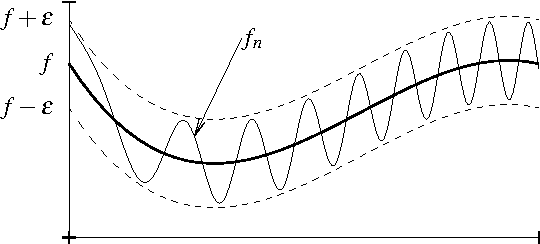
\includegraphics{figures/uniformconv}
\caption{In uniform convergence,
for $n \geq N$,
the functions $f_n$ are within a strip of $\pm\epsilon$ from $f$.%
\label{fig:uniformconv}}
\end{myfig}

It can easily be seen that uniform convergence implies pointwise
convergence.  The converse does not hold.

\begin{exbox}
\begin{exercise}
Prove that on $[0,1]$, the functions $x^n$ converge
pointwise but not uniformly.
\end{exercise}
\end{exbox}

\begin{defn} \label{def:unifnorm}
Let $f \colon S \to \R$ be a bounded function.  Define
\glsadd{not:uniformnorm}%
\begin{equation*}
\norm{f}_S
\overset{\text{def}}{=}
\sup \bigl\{ \sabs{f(x)} : x \in S \bigr\} .
\end{equation*}
$\norm{\cdot}_S$ is called the \emph{\myindex{uniform norm}}.
\end{defn}

\begin{prop}
A sequence of bounded functions $f_n \colon S \to \R$ converges
uniformly to $f \colon S \to \R$, if and only if
\begin{equation*}
\lim_{n\to\infty} \norm{f_n - f}_S = 0 .
\end{equation*}
\end{prop}

\begin{exbox}
\begin{exercise}
Prove the proposition.
\end{exercise}
\end{exbox}

Sometimes we say that \emph{$\{ f_n \}$ converges to $f$ in uniform norm}
\index{converges in uniform norm}
\index{uniform norm convergence}
instead of \emph{converges uniformly}.  The proposition
says that the two notions are the same thing.

Using uniform norm, we define Cauchy sequences in a similar way
as we define Cauchy sequences of real numbers.

\begin{defn}
Let $f_n \colon S \to \R$ be bounded functions.
The sequence is \emph{\myindex{Cauchy in the uniform norm}}
or \emph{\myindex{uniformly Cauchy}}
if for every $\epsilon > 0$, there exists an $N \in \N$ such
that for $m,k \geq N$ we have
\begin{equation*}
\norm{f_m-f_k}_S < \epsilon .
\end{equation*}
\end{defn}

\begin{prop} \label{prop:uniformcauchy}
Let $f_n \colon S \to \R$ be bounded functions.
Then $\{ f_n \}$ is Cauchy in the uniform norm if and only if
there exists an $f \colon S \to \R$ and $\{ f_n \}$ converges
uniformly to $f$.
\end{prop}

\begin{proof}
Let us first suppose $\{ f_n \}$ is Cauchy in the uniform norm.
Let us define $f$.  Fix $x$, then
the sequence $\{ f_n(x) \}$ is Cauchy because
\begin{equation*}
\abs{f_m(x)-f_k(x)}
\leq
\norm{f_m-f_k}_S .
\end{equation*}
Thus $\{ f_n(x) \}$ converges to some real number.  Define $f \colon S
\to \R$ by
\begin{equation*}
f(x) = \lim_{n \to \infty} f_n(x) .
\end{equation*}
The sequence
$\{ f_n \}$ converges pointwise to $f$.  To show that the convergence
is uniform, let $\epsilon > 0$ be given.  Find an $N$ such that
for $m, k \geq N$ we have
$\norm{f_m-f_k}_S < \nicefrac{\epsilon}{2}$.  In other words for
all $x$ we have
$\abs{f_m(x)-f_k(x)} < \nicefrac{\epsilon}{2}$.  We take the limit
as $k$ goes to infinity.  Then $\abs{f_m(x)-f_k(x)}$
goes to $\abs{f_m(x)-f(x)}$.
Consequently for all $x$ we get
\begin{equation*}
\abs{f_m(x)-f(x)} \leq \nicefrac{\epsilon}{2} < \epsilon .
\end{equation*}
And hence $\{ f_n \}$ converges uniformly.

For the other direction, suppose $\{ f_n \}$ converges uniformly to
$f$.  Given $\epsilon > 0$, find $N$ such that for all $n \geq N$,
$\abs{f_n(x)-f(x)} < \nicefrac{\epsilon}{4}$ for all $x \in S$.
Therefore for all $m, k \geq N$,
\begin{equation*}
\abs{f_m(x)-f_k(x)}
%= 
%\abs{f_m(x)-f(x)+f(x)-f_k(x)}
\leq
\abs{f_m(x)-f(x)}+\abs{f(x)-f_k(x)} < \nicefrac{\epsilon}{4} +
\nicefrac{\epsilon}{4} .
\end{equation*}
Take supremum over all $x$ to obtain
\begin{equation*}
\norm{f_m-f_k}_S \leq \nicefrac{\epsilon}{2} < \epsilon .  \qedhere
\end{equation*}
\end{proof}

\begin{exbox}
\begin{exercise}
Let $f$ and $g$ be bounded functions on $[a,b]$.  Prove 
\begin{equation*}
\norm{f+g}_S \leq \norm{f}_S + \norm{g}_S .
\end{equation*}
\end{exercise}

%\begin{exercise}
%\begin{exparts}
%\item
%Find the pointwise limit $\dfrac{e^{x/n}}{n}$ for $x \in \R$.
%\item
%Is the limit uniform on $\R$?
%\item
%Is the limit uniform on $[0,1]$?
%\end{exparts}
%\end{exercise}

\begin{exercise}
Suppose $f_n \colon S \to \R$ are functions that converge uniformly
to $f \colon S \to \R$.  Suppose $A \subset S$.  Show that
the sequence of restrictions $\{ f_n|_A \}$ converges uniformly to $f|_A$.
\end{exercise}

\begin{exercise}
\begin{exparts}
\item
Suppose $\{ f_n \}$ and $\{ g_n \}$ defined on some set $A$ converge to
$f$ and $g$ respectively pointwise, and let $a,b \in \R$.
Show that $\{ a f_n+ b g_n \}$ converges
pointwise to $a f+ b g$.
\item
Show the same for uniform convergence.
\end{exparts}
\end{exercise}

\begin{exercise}
Find an example of a sequence of functions $\{ f_n \}$ and $\{ g_n \}$
that converge uniformly to some $f$ and $g$ on some set $A$, but such that
$\{ f_ng_n \}$ (the multiple) does not converge uniformly to $fg$ on $A$.
\end{exercise}

\begin{exercise}
Suppose there exists a sequence of functions $\{ g_n \}$ uniformly
converging to $0$ on $A$.  Now suppose we have a sequence of functions
$\{ f_n \}$ and a function $f$ on $A$ such that
\begin{equation*}
\abs{f_n(x) - f(x)} \leq g_n(x) 
\end{equation*}
for all $x \in A$.  Show that $\{ f_n \}$ converges uniformly to $f$ on $A$.
\end{exercise}

\begin{exercise}
Let $\{ f_n \}$, $\{ g_n \}$ and $\{ h_n \}$ be sequences of functions on
$[a,b]$.  Suppose $\{ f_n \}$ and $\{ h_n \}$ converge uniformly to some function
$f \colon [a,b] \to \R$ and suppose $f_n(x) \leq g_n(x) \leq h_n(x)$
for all $x \in [a,b]$.  Show that $\{ g_n \}$ converges uniformly to $f$.
\end{exercise}

%\begin{exercise}
%Fix a continuous $h \colon [a,b] \to \R$.
%Let $f(x) = h(x)$ for $x \in [a,b]$,
%$f(x) = h(a)$ for $x < a$ and $f(x) = h(b)$ for all $x > b$.  First show
%that $f \colon \R \to \R$ is continuous.
%Let
%\begin{equation*}
%f_n(x) = \frac{n}{2} \int_{x-1/n}^{x+1/n} f(t) \, dt .
%\end{equation*}
%Show that $\{ f_n \}$ converges uniformly to $h$ on $[a,b]$.
%\end{exercise}


\begin{exercise}
Prove that
if a sequence of functions $f_n \colon S \to \R$
converge uniformly to a bounded function $f \colon S \to \R$,
then there exists an $N$ such that for all $n \geq N$, the $f_n$
are bounded.
\end{exercise}

%\begin{exercise}
%In \exampleref{example:geomsumptconv} we saw
%$\sum_{k=0}^\infty x^k$ converges pointwise to $\frac{1}{1-x}$ on
%$(-1,1)$.
%\begin{exparts}
%\item
%Show that for any $0 \leq c < 1$, the series
%$\sum_{k=0}^\infty x^k$ converges uniformly on $[-c,c]$.
%\item
%Show that the series $\sum_{k=0}^\infty x^k$ does not converge uniformly
%on $(-1,1)$.
%\end{exparts}
%\end{exercise}
\end{exbox}

\subsection{Continuity of the limit}

If we have a sequence $\{ f_n \}$ of continuous functions,
is the limit continuous?  We have seen that for pointwise
convergence, this need not be the case.
If we, however, require the convergence to be uniform, the limits can
be interchanged.

\begin{thm} \label{thm:uniformlimitcont}
Let $S$ be a metric space.
Let $\{ f_n \}$ be 
a sequence of continuous functions $f_n \colon S \to \R$ converging
uniformly to  $f \colon S \to \R$.  Then $f$ is continuous.
\end{thm}

\begin{proof}
Let $x \in S$ be fixed.  Let $\{ x_n \}$ be a sequence in $S$
converging to $x$.

Let $\epsilon > 0$ be given.
As $\{ f_k \}$ converges uniformly to $f$, we find a $k \in \N$ such that
\begin{equation*}
\abs{f_k(y)-f(y)} < \nicefrac{\epsilon}{3}
\end{equation*}
for all $y \in S$.  As $f_k$ is continuous at $x$,
we find an $N \in \N$ such that for $m \geq N$
we have 
\begin{equation*}
\abs{f_k(x_m)-f_k(x)} < \nicefrac{\epsilon}{3} .
\end{equation*}
Thus for
$m \geq N$ we have
\begin{equation*}
\begin{split}
\abs{f(x_m)-f(x)}
& =
\abs{f(x_m)-f_k(x_m)+f_k(x_m)-f_k(x)+f_k(x)-f(x)}
\\
& \leq
\abs{f(x_m)-f_k(x_m)}+
\abs{f_k(x_m)-f_k(x)}+
\abs{f_k(x)-f(x)}
\\
& <
\nicefrac{\epsilon}{3} +
\nicefrac{\epsilon}{3} +
\nicefrac{\epsilon}{3} = \epsilon .
\end{split}
\end{equation*}
Therefore $\{ f(x_m) \}$ converges to $f(x)$ and hence $f$ is continuous at
$x$.  As $x$ was arbitrary, $f$ is continuous everywhere.
\end{proof}

We say that a sequence of functions $f_n \colon S \to \R$
\emph{\myindex{converges uniformly on compact subsets}}
\index{uniform convergence on compact subsets}
if for every compact $K \subset S$
the sequence $\{ f_n \}$ converges uniformly on $K$.

\begin{cor} \label{cor:uniformkptlimitcont}
Let $S$ be a metric space.
If $f_n \colon S \to \R$ is a sequence of
continuous functions converging uniformly on compact subsets, then
the limit is continuous.
\end{cor}

\begin{exbox}
\begin{exercise}
Prove the corollary.
\end{exercise}
\end{exbox}

\subsection{Integral of the limit}

Again, if we simply require pointwise convergence, then the integral
of a limit of a sequence of functions need not be equal to the limit
of the integrals.

\begin{example}
Let $\chi_{T}$ be the characteristic function of a set $T$, that is $\chi_T(x) =
1$ if $x \in T$ and $\chi_T(x) = 0$ otherwise.
The functions $n \chi_{(0,\nicefrac{1}{n})}$ all integrate (on the interval
$[0,1]$) to $1$.  Their
pointwise limit is $0$ (whose integral is $0$).
\end{example}

If we require the convergence to be uniform, the limits can
be interchanged.

\begin{thm} \label{integralinterchange:thm}
Let $\{ f_n \}$ be a sequence of Riemann integrable
functions
$f_n \colon [a,b] \to \R$
converging uniformly to $f \colon [a,b]
\to \R$.  Then $f$ is Riemann integrable and
\begin{equation*}
\int_a^b f(x) \, dx = \lim_{n\to\infty} \int_a^b f_n(x) \, dx .
\end{equation*}
\end{thm}

In the following, let 
$\overline{\int_a^b} f(x)\, dx$ and 
$\underline{\int_a^b} f(x)\, dx$ denote the upper and lower Darboux integral.
The definition of the Riemann integral using Darboux sums and integrals is
beyond the scope of this book, but let us just mention that 
if the upper and lower Darboux integrals are equal, then a function is
Riemann integrable, and the common value is the integral.  Given this,
let us prove the theorem.

\begin{proof}
Let $\epsilon > 0$ be given.
As $f_n$ goes to $f$ uniformly, we find an $M \in \N$ such that
for all $n \geq M$ we have 
$\abs{f_n(x)-f(x)} < \frac{\epsilon}{2(b-a)}$ for all $x \in [a,b]$.
In particular, by reverse triangle inequality
$\abs{f(x)} < \frac{\epsilon}{2(b-a)} + \abs{f_n(x)}$ for all $x$,
hence $f$ is bounded
as $f_n$ is bounded.
Note that $f_n$ is integrable and compute
\begin{align*}
\overline{\int_a^b} & f(x) \, dx
-
\underline{\int_a^b} f(x) \, dx
\\
& =
\overline{\int_a^b} \bigl( f(x) - f_n(x) + f_n(x) \bigr) \, dx
-
\underline{\int_a^b} \bigl( f(x) - f_n(x) + f_n(x) \bigr) \, dx
\displaybreak[0]\\
& \leq
\overline{\int_a^b} \bigl( f(x) - f_n(x) \bigr) \, dx +  \overline{\int_a^b}
f_n(x) \, dx
-
\underline{\int_a^b} \bigl( f(x) - f_n(x) \bigr) \, dx -
\underline{\int_a^b} f_n(x) \, dx
\displaybreak[0]\\
& =
\overline{\int_a^b} \bigl( f(x) - f_n(x) \bigr)\, dx +  \int_a^b f_n(x) \, dx
-
\underline{\int_a^b} \bigl( f(x) - f_n(x) \bigr)\, dx -  \int_a^b f_n(x) \, dx
\displaybreak[0]\\
& =
\overline{\int_a^b} \bigl( f(x) - f_n(x) \bigr)\, dx
-
\underline{\int_a^b} \bigl( f(x) - f_n(x) \bigr)\, dx
\\
& \leq
\frac{\epsilon}{2(b-a)} (b-a) + 
\frac{\epsilon}{2(b-a)} (b-a) = \epsilon .
\end{align*}
The second inequality follows from
the fact that for all $x \in [a,b]$ we have
$\frac{-\epsilon}{2(b-a)} < f(x)-f_n(x) < \frac{\epsilon}{2(b-a)}$.
As $\epsilon > 0$ was arbitrary, $f$ is Riemann integrable.

We compute $\int_a^b f(x)\,dx$.
For $n \geq M$ ($M$ is the same as above),
\begin{equation*}
\begin{split}
\abs{\int_a^b f(x)\,dx - \int_a^b f_n(x)\,dx} & = 
\abs{ \int_a^b \bigl(f(x) - f_n(x)\bigr)\,dx}
\\
& \leq
\frac{\epsilon}{2(b-a)} (b-a) = \frac{\epsilon}{2} < \epsilon .
\end{split}
\end{equation*}
Therefore $\bigl\{ \int_a^b f_n(x) \,dx \bigr\}$ converges to $\int_a^b f(x) \,dx$.
\end{proof}

%\begin{example}
%Using \thmref{integralinterchange:thm}, we compute
%\begin{equation*}
%\lim_{n\to\infty} \int_0^1 \frac{nx+ \sin(nx^2)}{n} \,dx
%=
%\int_0^1
%x \,dx = \nicefrac{1}{2} .
%\end{equation*}
%It is impossible to compute the integrals for any particular $n$ using 
%calculus as $\sin(nx^2)$ has no closed-form antiderivative.
%\end{example}

\begin{remark}
While we will not require the Lebesgue integral in this book, note that
for Lebesgue integral a much stronger convergence theorem holds.  In
particular, the dominated convergence theorem implies that if
$\{ f_n \}$ is a sequence of measurable functions on $[a,b]$,
converging pointwise to $f \colon [a,b] \to \R$, and such that
$\{ f_n \}$ is uniformly bounded (there is a single $B \in \R$ such that
$\snorm{f_n}_{[a,b]} \leq B$ for all $n$), then
\begin{equation*}
\int_a^b f(x) \, dx = \lim_{n\to\infty} \int_a^b f_n(x) \, dx .
\end{equation*}
Where of course all the integrals would have to be the Lebesgue integrals,
not the Riemann integrals.  The pointwise limit of Riemann integrable
functions need not even be Riemann integrable.
\end{remark}

\begin{exbox}
\begin{exercise}
Compute
$\displaystyle \lim_{n\to\infty} \int_1^2 e^{-nx^2} ~dx$.
\end{exercise}

\begin{exercise}
Find a sequence of Riemann integrable functions $f_n \colon [0,1] \to \R$ such
that $\{ f_n \}$ converges to zero pointwise, and such that
\begin{exparts}
\item
$\bigl\{ \int_0^1 f_n(x)\,dx \bigr\}_{n=1}^\infty$ increases without bound,
\item
$\bigl\{ \int_0^1 f_n(x)\,dx \bigr\}_{n=1}^\infty$ is the sequence $-1,1,-1,1,-1,1, \ldots$.
\end{exparts}
\end{exercise}
\end{exbox}

\subsection{Derivative of the limit}

While uniform convergence is enough to swap limits with integrals, it is not,
however, enough to swap limits with derivatives, unless you also have
uniform convergence of the derivatives themselves.

\begin{example}
Let $f_n(x) = \frac{\sin(nx)}{n}$.
Then $f_n$ converges uniformly to $0$.
See \figureref{fig:conv1nsinxn}.
The derivative of the limit is $0$.
But $f_n'(x) = \cos(nx)$,
which does not converge even pointwise,
for example $f_n'(\pi) = {(-1)}^n$.
Furthermore, $f_n'(0) = 1$ for all $n$, which does converge, but not to $0$.
\begin{myfig}
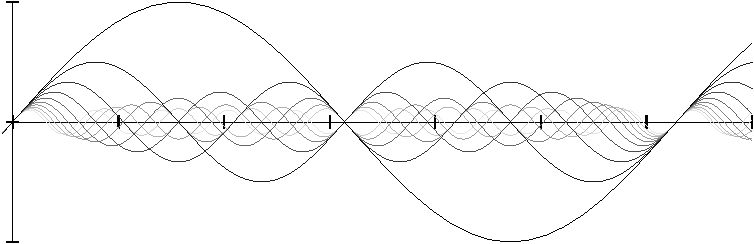
\includegraphics{figures/conv1nsinxn}
\caption{Graphs of $\frac{\sin(nx)}{n}$ for
$n=1,2,\ldots,10$, with higher $n$ in lighter gray.%
\label{fig:conv1nsinxn}}
\end{myfig}
\end{example}

The following theorem is true even if 
we do not assume continuity of the derivatives, but the proof is more
difficult.

\begin{thm} \label{thm:dersconverge}
Let $I$ be a bounded interval and let
$f_n \colon I \to \R$ be continuously differentiable functions.
Suppose $\{ f_n' \}$ converges uniformly to $g \colon I \to \R$,
and suppose $\{ f_n(c) \}_{n=1}^\infty$ is a
convergent sequence for some $c \in I$.  Then $\{ f_n \}$ converges uniformly to 
a continuously differentiable function $f \colon I \to \R$, and $f' = g$.
\end{thm}

\begin{proof}
Define $f(c) = \lim_{n\to \infty} f_n(c)$.
As $f_n'$ are continuous and hence Riemann integrable,
then
via the fundamental theorem of calculus, we find that for $x \in I$,
\begin{equation*}
f_n(x) = f_n(c) + \int_c^x f_n' (t)\, dt.
\end{equation*}
As $\{ f_n' \}$ converges uniformly on $I$, it converges uniformly
on $[c,x]$ (or $[x,c]$ if $x < c$).
Therefore, we find that the limit on the right hand side exists.
Let us define $f$ at the remaining points by this limit:
\begin{equation*}
f(x) =
\lim_{n\to\infty} f_n(c) + \lim_{n\to\infty} \int_c^x f_n' (t)\, dt
=
f(c) + \int_c^x g(t)\,dt .
\end{equation*}
The function $g$ is continuous, being the uniform limit of continuous
functions.  Hence $f$ is differentiable and $f'(x) = g(x)$ for all $x \in I$
by the second form of the fundamental theorem.

It remains to prove
uniform convergence.
Suppose $I$ has a lower bound $a$ and upper bound $b$.
Let $\epsilon > 0$ be given.  Take $M$
such that for $n \geq M$ we have
$\abs{f(c)-f_n(c)} < \nicefrac{\epsilon}{2}$,
and
$\abs{g(x)-f_n'(x)} < \nicefrac{\epsilon}{2(b-a)}$
for all $x \in I$.  Then
\begin{equation*}
\begin{split}
\abs{f(x) - f_n(x)} & =
\abs{f(c) + \int_c^x g - f_n(c) - \int_c^x f_n'(t)\,dt}
\\
& \leq
\abs{f(c) - f_n(c)} + \abs{\int_c^x g(t)\,dt - \int_c^x f_n'(t)\,dt}
\\
& =
\abs{f(c) - f_n(c)} + \abs{\int_c^x \bigl(g(t) - f_n'(t)\bigr) \, dt}
\\
& <
\frac{\epsilon}{2}
+
\frac{\epsilon}{2(b-a)}
(b-a)
=\epsilon. \qedhere
\end{split}
\end{equation*}
\end{proof}

The proof goes through without boundedness of $I$, except for the
uniform convergence of $f_n$ to $f$.  As an example suppose $I = \R$ and let
$f_n(x) = \nicefrac{x}{n}$.  Then $f_n'(x)=\nicefrac{1}{n}$, which
converges uniformly to $0$.  However, $\{f_n\}$ converges to $0$ only pointwise.

\begin{exbox}
\begin{exercise}
Find an explicit example of a sequence of
differentiable functions on $[-1,1]$ that converge uniformly to
a function $f$ such that $f$ is not differentiable.
Hint:
There are many possibilities,
simplest is perhaps to combine $\abs{x}$ and $\frac{n}{2}x^2 +
\frac{1}{2n}$, another is to
consider $\sqrt{x^2+{(\nicefrac{1}{n})}^2}$.  Show that these functions are differentiable,
converge uniformly, and then show that the limit is not differentiable.
\end{exercise}

\begin{exercise}
Let $f_n(x) = \frac{x^n}{n}$.  Show that $\{ f_n \}$ converges uniformly to
a differentiable function $f$ on $[0,1]$ (find $f$).  However, show that
$f'(1) \not= \lim\limits_{n\to\infty} f_n'(1)$.
\end{exercise}
\end{exbox}

%%%%%%%%%%%%%%%%%%%%%%%%%%%%%%%%%%%%%%%%%%%%%%%%%%%%%%%%%%%%%%%%%%%%%%%%%%%%%%

\section{Continuity and derivatives under the integral}
\label{sec:contlimitsunderint}

\subsection{Continuity}

Let us prove a useful criterion for
continuity of functions defined by integrals.  Let $f(x,y)$ be a function of two variables and define
\begin{equation*}
g(y) = \int_a^b f(x,y) \,dx .
\end{equation*}
Question is, is $g$ is continuous?
We are really asking when do two limiting operations commute,
which is not always possible, so some extra hypothesis
is necessary.  A useful sufficient (but not
necessary) condition is that $f$ is continuous on a closed rectangle.

\begin{prop} \label{prop:integralcontcont}
If $f \colon [a,b] \times [c,d] \to \R$ is a continuous function,
then $g \colon [c,d] \to \R$ defined by
\begin{equation*}
g(y) = \int_a^b f(x,y) \,dx  \qquad \text{is continuous}.
\end{equation*}
\end{prop}

\begin{proof}
Fix $y \in [c,d]$, and let $\{ y_n \}$ be a sequence in $[c,d]$
converging to $y$.
Let $\epsilon > 0$ be given.
As $f$ is continuous on $[a,b] \times [c,d]$, which is compact, $f$
is uniformly continuous.  
In particular, there exists a $\delta > 0$ such that
whenever $\widetilde{y} \in [c,d]$ and
$\abs{\widetilde{y}-y} < \delta$ we have
$\abs{f(x,\widetilde{y})-f(x,y)} < \epsilon$ for all $x \in [a,b]$.
If we let $h_n(x)= f(x,y_n)$ and $h(x) = f(x,y)$,
we have just shown that
$h_n \colon [a,b] \to \R$ converges uniformly 
to
$h \colon [a,b] \to \R$ as $n$ goes to $\infty$.
Uniform convergence implies the limit can be taken underneath the integral.
So
\begin{equation*}
\lim_{n\to \infty}
g(y_n)
=
\lim_{n\to \infty}
\int_a^b 
f(x,y_n) \,dx 
= 
\int_a^b 
\lim_{n\to \infty}
f(x,y_n) \,dx 
= 
\int_a^b 
f(x,y) \,dx = g(y) . \qedhere
\end{equation*}
\end{proof}

In applications, if we are interested in continuity at $y_0$, we just
need to apply the proposition in $[a,b] \times [y_0-\epsilon,y_0+\epsilon]$
for some small $\epsilon > 0$.  For example, if $f$ is continuous in
$[a,b] \times \R$, then $g$ is continuous on $\R$.

\begin{exbox}
\begin{exercise} \label{exercise:integralcontcontextra}
Prove a stronger version of \propref{prop:integralcontcont}:
If $f \colon (a,b) \times (c,d) \to \R$ is a bounded continuous function,
then $g \colon [c,d] \to \R$ defined by
\begin{equation*}
g(y) = \int_a^b f(x,y) \,dx  \qquad \text{is continuous}.
\end{equation*}
Hint: First integrate over $[a+\nicefrac{1}{n},b-\nicefrac{1}{n}]$.
\end{exercise}
\end{exbox}

\subsection{Differentiation under the integral}
\label{subsec:diffunderint}

Let $f(x,y)$ be a function of two variables and
\begin{equation*}
g(y) = \int_a^b f(x,y) \,dx .
\end{equation*}
If $f$ is continuous on the compact rectangle $[a,b] \times [c,d]$, then
\propref{prop:integralcontcont}
says that $g$ is continuous on $[c,d]$.

Suppose $f$ is differentiable in $y$.  The main question we want to
ask is when can we ``differentiate under the integral,'' that is,
when is it true that $g$ is differentiable and its derivative is
\begin{equation*}
g'(y) \overset{?}{=} \int_a^b \frac{\partial f}{\partial y}(x,y) \,dx .
\end{equation*}
Differentiation is a limit and therefore we are really asking when do the
two limiting operations of integration and differentiation commute.
This is not always possible and some extra hypothesis is
necessary.  In particular, the first
question we would face is the integrability of
$\frac{\partial f}{\partial y}$, but the formula can fail even if
$\frac{\partial f}{\partial y}$ is integrable as a function of $x$ for every
fixed $y$.

Let us prove a simple, but perhaps the most useful version of this theorem.

\begin{thm}[\myindex{Leibniz integral rule}]
\label{thm:Leibnizrule}
Suppose $f \colon [a,b] \times [c,d] \to \R$ is a continuous function,
such that $\frac{\partial f}{\partial y}$ exists for all $(x,y) \in [a,b]
\times [c,d]$ and is continuous.  Define
\begin{equation*}
g(y) = \int_a^b f(x,y) \,dx .
\end{equation*}
Then $g \colon [c,d] \to \R$ is continuously differentiable and
\begin{equation*}
g'(y) = \int_a^b \frac{\partial f}{\partial y}(x,y) \,dx .
\end{equation*}
\end{thm}

The hypotheses on $f$ and $\frac{\partial f}{\partial y}$ can be
weakened, see e.g.\ \exerciseref{exercise:strongerleibniz},
but not dropped outright.
The main point in the proof is for
$\frac{\partial f}{\partial y}$ to exist and be continuous for all $x$
up to the ends, but we only need a small
interval in the $y$ direction.  In applications, we often make $[c,d]$ be a
small interval around the point where we need to differentiate.

\begin{proof}
Fix $y \in [c,d]$ and let $\epsilon > 0$ be given.
As $\frac{\partial f}{\partial y}$ is continuous on $[a,b] \times [c,d]$ it
is uniformly continuous.  In particular, there exists $\delta > 0$ such that
whenever $y_1 \in [c,d]$ with
$\abs{y_1-y} < \delta$ and all $x \in [a,b]$ we have
\begin{equation*}
\abs{\frac{\partial f}{\partial y}(x,y_1)-\frac{\partial f}{\partial y}(x,y)} < \epsilon .
\end{equation*}

Suppose $h$ is such that $y+h \in [c,d]$ and $\abs{h} < \delta$.
Fix $x$ for a moment
and apply the mean value theorem to find a $y_1$ between $y$ and $y+h$ such that
\begin{equation*}
\frac{f(x,y+h)-f(x,y)}{h}
=
\frac{\partial f}{\partial y}(x,y_1) .
\end{equation*}
As $\abs{y_1-y} \leq \abs{h} < \delta$,
\begin{equation*}
\abs{
\frac{f(x,y+h)-f(x,y)}{h}
-
\frac{\partial f}{\partial y}(x,y) 
}
=
\abs{
\frac{\partial f}{\partial y}(x,y_1) 
-
\frac{\partial f}{\partial y}(x,y) 
}
< \epsilon .
\end{equation*}
This argument worked for every $x \in [a,b]$.  Therefore, as a function of
$x$
\begin{equation*}
x \mapsto \frac{f(x,y+h)-f(x,y)}{h}
\quad
\text{converges uniformly to}
\quad
x \mapsto \frac{\partial f}{\partial y}(x,y)
\quad
\text{as } h \to 0 .
\end{equation*}
We defined uniform convergence for sequences although the idea is the
same.  You may replace $h$ with a sequence of nonzero 
numbers $\{ h_n \}$
converging to $0$ such that $y+h_n \in [c,d]$ and let $n \to \infty$.

Consider the difference quotient of $g$,
\begin{equation*}
\frac{g(y+h)-g(y)}{h}
=
\frac{\int_a^b f(x,y+h) \,dx -
\int_a^b f(x,y) \,dx }{h}
=
\int_a^b \frac{f(x,y+h)-f(x,y)}{h} \,dx .
\end{equation*}
Uniform convergence implies the limit can be taken underneath the integral.
So
\begin{equation*}
\lim_{h\to 0}
\frac{g(y+h)-g(y)}{h}
= 
\int_a^b 
\lim_{h\to 0}
\frac{f(x,y+h)-f(x,y)}{h} \,dx 
=
\int_a^b 
\frac{\partial f}{\partial y}(x,y) \,dx .
\end{equation*}
Then $g'$ is continuous on $[c,d]$ by
\propref{prop:integralcontcont}.
\end{proof}

\begin{example} \label{example:counterexamplediffunder}
Suppose we start with
\begin{equation*}
\int_0^{1} \frac{x-1}{\ln(x)} \,dx .
\end{equation*}
The function under the integral 
extends to be continuous on $[0,1]$, and hence
the integral exists, see \exerciseref{exercise:counterexamplediffunder}.  Trouble is finding it.  Introduce a parameter $y$
and define a function:
\begin{equation*}
g(y) = \int_0^{1} \frac{x^y-1}{\ln(x)} \,dx .
\end{equation*}
The function
$\frac{x^y-1}{\ln(x)}$
also extends to a continuous function of $x$ and $y$
for $(x,y) \in [0,1] \times [0,1]$ (also in the exercise).
See \figureref{fig:diffunderexample}.
\begin{myfig}
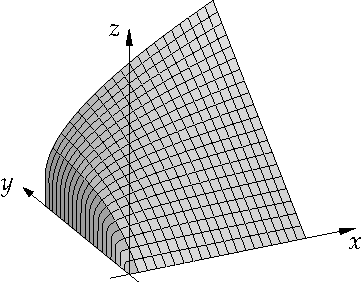
\includegraphics{figures/diffunderexample}
\caption{The graph $z= \frac{x^y-1}{\ln(x)}$ on $[0,1] \times [0,1]$.\label{fig:diffunderexample}}
\end{myfig}


Therefore
$g$ is a continuous function of on $[0,1]$, and $g(0) = 0$.
For any $\epsilon > 0$, the $y$ derivative of the integrand, $x^y$,
is continuous on $[0,1] \times [\epsilon,1]$.  Therefore,
for $y >0$ we may differentiate under the integral sign
\begin{equation*}
g'(y) =
\int_0^{1} \frac{\ln(x) x^y}{\ln(x)} \,dx 
=
\int_0^{1} x^y \,dx =
\frac{1}{y+1} .
\end{equation*}
We need to figure out $g(1)$, knowing $g'(y) = \frac{1}{y+1}$ and $g(0) =
0$.  By elementary calculus we find $g(1) = \int_0^1 g'(y)\,dy = \ln(2)$.  Therefore
\begin{equation*}
\int_0^{1} \frac{x-1}{\ln(x)} \,dx  = \ln(2).
\end{equation*}
\end{example}

\begin{exbox}
\begin{exercise} \label{exercise:counterexamplediffunder}
Prove the two statements that were asserted in
\exampleref{example:counterexamplediffunder}:
\begin{exparts}
\item
Prove $\frac{x-1}{\ln(x)}$ extends to a continuous function of
$[0,1]$.  That is, there exists a continuous function on $[0,1]$
that equals $\frac{x-1}{\ln(x)}$ on $(0,1)$.
\item
Prove $\frac{x^y-1}{\ln(x)}$ extends to a continuous function
on $[0,1] \times [0,1]$.
\end{exparts}
\end{exercise}

\begin{exercise}
Suppose $h \colon \R \to \R$ is a continuous function.  Suppose $g
\colon \R \to \R$ is which is continuously differentiable and compactly
supported.  That is there exists some $M > 0$ such that $g(x) = 0$ whenever
$\abs{x} \geq M$.  Define
\begin{equation*}
f(x) = \int_{-\infty}^\infty h(y)g(x-y) \, dy  .
\end{equation*}
Show that $f$ is differentiable.
\end{exercise}

\begin{exercise}
Suppose $f \colon \R \to \R$ is an infinitely differentiable function (all derivatives exist)
such that $f(0) = 0$.  Then show that there exists an infinitely
differentiable function $g \colon \R \to \R$ such that $f(x) = x\,g(x)$.  Finally show that
if $f'(0) \not= 0$, then $g(0) \not= 0$.\\
Hint: First write
$f(x) = \int_0^x f'(s) \,ds$ and then rewrite the integral to go
from $0$ to $1$.
\end{exercise}

\begin{exercise} \label{exercise:severalvariableLiebniz}
Let $U \subset \R^n$ be an open set and suppose
$f(x,y_1,y_2,\ldots,y_n)$ is a continuous
function defined on $[0,1] \times U \subset \R^{n+1}$.
Suppose
$\frac{\partial f}{\partial y_1},
\frac{\partial f}{\partial y_2},\ldots,
\frac{\partial f}{\partial y_n}$
exist and are continuous on $[0,1] \times U$.
Then prove that $F \colon U \to \R$ defined by
\begin{equation*}
F(y_1,y_2,\ldots,y_n) =
\int_0^1
f(x,y_1,y_2,\ldots,y_n)
\, dx
\end{equation*}
is continuously differentiable (the partial derivatives exist and are
continuous).
\end{exercise}

\begin{exercise}
Work out the following counterexample:  Let
\begin{equation*}
f(x,y) =
\begin{cases}
\frac{xy^3}{{(x^2+y^2)}^2} & \text{if } x\not=0 \text{ or  } y\not= 0,\\
0 & \text{if } x=0 \text{ and } y=0.
\end{cases}
\end{equation*}
\begin{exparts}
\item
Prove that for any fixed $y$ the function $x \mapsto f(x,y)$ is
Riemann integrable on $[0,1]$ and
\begin{equation*}
g(y) = \int_0^1 f(x,y) \, dx = \frac{y}{2y^2+2} .
\end{equation*}
Therefore $g'(y)$ exists and we get the continuous function
\begin{equation*}
g'(y) = \frac{1-y^2}{2{(y^2+1)}^2} .
\end{equation*}
\item
Prove $\frac{\partial f}{\partial y}$ exists at all $x$ and $y$ and
compute it.
\item
Show that for all $y$
\begin{equation*}
\int_0^1 \frac{\partial f}{\partial y} (x,y) \, dx
\end{equation*}
exists, but
\begin{equation*}
g'(0) \not= \int_0^1 \frac{\partial f}{\partial y} (x,0) \, dx .
\end{equation*}
\end{exparts}
\end{exercise}

\begin{exercise}
Work out the following counterexample:  Let
\begin{equation*}
f(x,y) =
\begin{cases}
x \,\sin \left(\frac{y}{x^2+y^2}\right) & \text{if } (x,y) \not= (0,0),\\
0 & \text{if } (x,y)=(0,0).
\end{cases}
\end{equation*}
\begin{exparts}
\item
Prove $f$ is continuous on all of $\R^2$.
Therefore the following function is well-defined for every $y \in \R$:
\begin{equation*}
g(y) = \int_0^1 f(x,y) \, dx .
\end{equation*}
\item
Prove $\frac{\partial f}{\partial y}$ exists for all $(x,y)$,
but is not continuous at $(0,0)$.
\item
Show that $\int_0^1 \frac{\partial f}{\partial y}(x,0) \, dx$ does not
exist even if we take improper integrals, that is,
that the limit
$\lim\limits_{h \to 0^+} \int_h^1 \frac{\partial f}{\partial y}(x,0) \, dx$
does not exist.
\end{exparts}
Note: Feel free to use what you know about sine and cosine from calculus.
\end{exercise}

\begin{exercise} \label{exercise:strongerleibniz}
Strengthen the Leibniz integral rule in the following way.
Suppose $f \colon (a,b) \times (c,d) \to \R$ is a bounded continuous function,
such that $\frac{\partial f}{\partial y}$ exists for all $(x,y) \in (a,b)
\times (c,d)$ and is continuous and bounded.  Define
\begin{equation*}
g(y) = \int_a^b f(x,y) \,dx .
\end{equation*}
Then $g \colon (c,d) \to \R$ is continuously differentiable and
\begin{equation*}
g'(y) = \int_a^b \frac{\partial f}{\partial y}(x,y) \,dx .
\end{equation*}
Hint: See also \exerciseref{exercise:integralcontcontextra} and
\thmref{thm:dersconverge}.
\end{exercise}
\end{exbox}

%%%%%%%%%%%%%%%%%%%%%%%%%%%%%%%%%%%%%%%%%%%%%%%%%%%%%%%%%%%%%%%%%%%%%%%%%%%%%%

\section{The derivative in several real variables} \label{sec:derinsv}

\subsection{The derivative}

In the following, the norm $\snorm{\cdot}$ of a vector in $\R^n$
is the Euclidean norm $\snorm{x} = \sqrt{x_1^2+\cdots+x_n^2}$.
When applied to a linear mapping (a matrix) it is the
\emph{\myindex{operator norm}}:
\begin{equation*}
\snorm{A} \overset{\text{def}}{=} \sup_{\snorm{x} = 1} \snorm{Ax} .
\end{equation*}
The following exercise collects some key facts about the operator norm
for the reader who has not seen this norm yet.

\begin{exbox}
\begin{exercise}
\begin{exparts} 
\item
Prove that if $A$ is a linear mapping between finite dimensional vector
spaces, then $\snorm{A} < \infty$.
\item
Prove that if $A$ is a linear mapping of vector spaces, then
$\snorm{Ax} \leq \snorm{A} \snorm{x}$.
\end{exparts} 
\end{exercise}
\end{exbox}

For a function $f \colon \R \to \R$, 
the derivative at $x$ exists if 
there is a number $a$ (the derivative of $f$ at $x$) such that
\begin{equation*}
\lim_{h \to 0} \abs{\frac{f(x+h)-f(x)}{h} - a} =
\lim_{h \to 0} \frac{\sabs{f(x+h)-f(x) - ah}}{\sabs{h}}
= 0.
\end{equation*}

Multiplying by $a$ is a linear map in one dimension:
$h \mapsto ah$.  Let us extend this idea to more variables.

\begin{defn}
Let $U \subset \R^n$ be an open subset and $f \colon U \to \R^m$.  We
say $f$ is \emph{(real) differentiable\index{real differentiable}}
at $x \in U$ if there exists
a linear $A \colon \R^n \to \R^m$ such that
\begin{equation*}
\lim_{\substack{h \to 0\\h\in \R^n}}
\frac{\snorm{f(x+h)-f(x) - Ah}}{\snorm{h}} = 0 .
\end{equation*}
We write $Df|_x = A$\glsadd{not:mvder} and
we say $A$ is the \emph{(real) derivative\index{real derivative}} of $f$ at $x$.
When $f$ is \emph{(real) differentiable} at
every $x \in U$, we say that $f$ is (real) differentiable.  See
\figureref{fig:svder}.
\end{defn}

\begin{myfig}
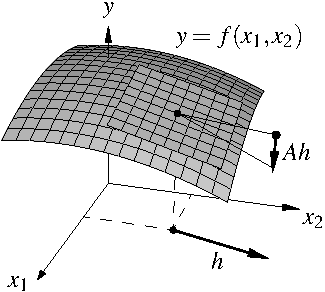
\includegraphics{figures/svder}
\caption{Illustration of a derivative for a function $f \colon \R^2 \to \R$.  The vector $h$ is shown
in the $x_1x_2$-plane based at $(x_1,x_2)$, and the vector
$Ah \in \R^1$ is shown along the $y$ direction.\label{fig:svder}}
\end{myfig}

We cheated somewhat and said that $A$
is \emph{the} derivative, let us prove that we were justified.

\begin{prop}
Let $U \subset \R^n$ be an open subset and $f \colon U \to \R^m$.  Suppose
$x \in U$ and there exist linear
$A,B \colon \R^n \to \R^m$ such that
\begin{equation*}
\lim_{h \to 0}
\frac{\snorm{f(x+h)-f(x) - Ah}}{\snorm{h}} = 0
\qquad \text{and} \qquad
\lim_{h \to 0}
\frac{\snorm{f(x+h)-f(x) - Bh}}{\snorm{h}} = 0 .
\end{equation*}
Then $A=B$.
\end{prop}

\begin{proof}
Suppose $h \in \R^n$, $h \not= 0$.  Compute
\begin{equation*}
\begin{split}
\frac{\snorm{(A-B)h}}{\snorm{h}} & =
\frac{\snorm{f(x+h)-f(x) - Ah - (f(x+h)-f(x) - Bh)}}{\snorm{h}} \\
& \leq
\frac{\snorm{f(x+h)-f(x) - Ah}}{\snorm{h}} + \frac{\snorm{f(x+h)-f(x) -
Bh}}{\snorm{h}} .
\end{split}
\end{equation*}
So 
$\frac{\snorm{(A-B)h}}{\snorm{h}} = \norm{(A-B)\frac{h}{\snorm{h}}} \to 0$
as $h \to 0$.  For an arbitrarily small $h$, $\frac{h}{\snorm{h}}$ is
on the unit sphere, and a linear mapping vanishing on the unit sphere is
zero everywhere.
\end{proof}

\begin{example}
If $f(x) = Ax$ for a linear mapping $A$, then
$Df|_x = A$:
\begin{equation*}
\frac{\snorm{f(x+h)-f(x) - Ah}}{\snorm{h}}
=
\frac{\snorm{A(x+h)-Ax - Ah}}{\snorm{h}}
=
\frac{0}{\snorm{h}} = 0 .
\end{equation*}
\end{example}

\begin{example}
Let $f \colon \R^2 \to \R^2$ be defined by
\begin{equation*}
f(x,y) = \bigl(f_1(x,y),f_2(x,y)\bigr) = (1+x+2y+x^2,2x+3y+xy).
\end{equation*}
Let us show that $f$ is differentiable at the origin and let us 
compute the derivative,
directly using the definition.  If the
derivative exists, it can be
represented by a $2$-by-$2$ matrix
$\left[\begin{smallmatrix}a&b\\c&d\end{smallmatrix}\right]$.  Suppose $h =
(h_1,h_2)$.  We need the following expression to go to zero.
\begin{multline*}
\frac{\snorm{
f(h_1,h_2)-f(0,0)
-
(ah_1 +bh_2 , ch_1+dh_2)}
}{\snorm{(h_1,h_2)}}
=
\\
\frac{\sqrt{
{\bigl((1-a)h_1 + (2-b)h_2 + h_1^2\bigr)}^2
+
{\bigl((2-c)h_1 + (3-d)h_2 + h_1h_2\bigr)}^2}}{\sqrt{h_1^2+h_2^2}} .
\end{multline*}
If we choose $a=1$, $b=2$, $c=2$, $d=3$, the expression becomes
\begin{equation*}
\frac{\sqrt{
h_1^4 + h_1^2h_2^2}}{\sqrt{h_1^2+h_2^2}}
=
\sabs{h_1}
\frac{\sqrt{
h_1^2 + h_2^2}}{\sqrt{h_1^2+h_2^2}}
= \sabs{h_1} .
\end{equation*}
And this expression does indeed go to zero as $h \to 0$.  The
function $f$ is differentiable at the origin and 
the derivative $Df|_0$ is represented by the matrix
$\left[\begin{smallmatrix}1&2\\2&3\end{smallmatrix}\right]$.
\end{example}

\begin{prop}
Let $U \subset \R^n$ be open and $f \colon U \to \R^m$ be
differentiable at $p \in U$.  Then $f$ is continuous at $p$.
\end{prop}

\begin{proof}
Another way to write the differentiability of $f$ at $p$ is to first write
\begin{equation*}
r(h) = f(p+h)-f(p) - Df|_p h ,
\end{equation*}
and $\frac{\snorm{r(h)}}{\snorm{h}}$ must go to zero as $h \to 0$.
So
$r(h)$ itself must go to zero.  The mapping $h \mapsto Df|_p h$
is a linear mapping between finite dimensional spaces, it is
therefore continuous
and goes to zero as $h \to 0$.  So
$f(p+h)$ must go to $f(p)$ as $h \to 0$.
\end{proof}

The derivative is itself a linear operator on the space of differentiable
functions.

\begin{prop}
Suppose $U \subset \R^n$ is open,
$f \colon U \to \R^m$ and
$g \colon U \to \R^m$ are differentiable at $p$,
and $\alpha \in \R$.  Then the functions $f+g$ and $\alpha f$
are differentiable at $p$ and
\begin{equation*}
D(f+g)|_p = Df|_p + Dg|_p , \qquad \text{and} \qquad D(\alpha f)|_p = \alpha
Df|_p .
\end{equation*}
\end{prop}

\begin{proof}
Let $h \in \R^n$, $h \not= 0$.  The proposition follows from the following
estimates:
\begin{multline*}
\frac{\norm{f(p+h)+g(p+h)-\bigl(f(p)+g(p)\bigr) - \bigl(Df|_p + Dg|_p\bigr)h}}{\snorm{h}}
\\
\leq
\frac{\norm{f(p+h)-f(p) - Df|_ph}}{\snorm{h}}
+
\frac{\norm{g(p+h)-g(p) - Dg|_ph}}{\snorm{h}} ,
\end{multline*}
and
\begin{equation*}
\frac{\norm{\alpha f(p+h) - \alpha f(p) - \alpha Df|_p h}}{\snorm{h}}
=
\sabs{\alpha} \frac{\norm{f(p+h))-f(p) - Df|_ph}}{\snorm{h}} .
\qedhere
\end{equation*}
\end{proof}

If $A \colon X \to Y$ and $B \colon Y \to Z$ are linear maps, then 
they are their own derivative.  The composition
$BA$, a linear map from $X$ to $Z$, is also its own derivative, and
so the derivative of the composition is the composition
of the derivatives.  As differentiable maps are ``infinitesimally close''
to linear maps, they have the same property:

\begin{thm}[Chain rule]\index{chain rule!real derivative} \label{thm:realchain}
Let $U \subset \R^n$ be open and let $f \colon U \to \R^m$ be
differentiable at $p \in U$.  Let $V \subset \R^m$ be open,
$f(U) \subset V$ and let $g \colon V \to \R^\ell$ be differentiable
at $f(p)$.  Then
\begin{equation*}
F(x) = g\bigl(f(x)\bigr)
\end{equation*}
is differentiable at $p$ and
\begin{equation*}
DF|_p = Dg|_{f(p)} Df|_p .
\end{equation*}
\end{thm}

\begin{proof}
Let $A = Df|_p$ and $B = Dg|_{f(p)}$.  Take $h \in \R^n$
and write $q = f(p)$, $k = f(p+h)-f(p)$.  Let
\begin{equation*}
r(h) = f(p+h)-f(p) - A h . %= k - Ah.
\end{equation*}
Then $r(h) = k-Ah$ or $Ah = k-r(h)$, and $f(p+h) = q+k$.
\begin{equation*}
\begin{split}
\frac{\snorm{F(p+h)-F(p) - BAh}}{\snorm{h}}
& =
\frac{\snorm{g\bigl(f(p+h)\bigr)-g\bigl(f(p)\bigr) - BAh}}{\snorm{h}}
\\
& =
\frac{\snorm{g(q+k)-g(q) - B\bigl(k-r(h)\bigr)}}{\snorm{h}}
\\
& \leq
\frac
{\snorm{g(q+k)-g(q) - Bk}}
{\snorm{h}}
+
\snorm{B}
\frac
{\snorm{r(h)}}
{\snorm{h}}
\\
& =
\frac
{\snorm{g(q+k)-g(q) - Bk}}
{\snorm{k}}
\frac
{\snorm{f(p+h)-f(p)}}
{\snorm{h}}
+
\snorm{B}
\frac
{\snorm{r(h)}}
{\snorm{h}} .
\end{split}
\end{equation*}
First, $\snorm{B}$ is constant and $f$ is differentiable at $p$,
so
the term $\snorm{B}\frac{\snorm{r(h)}}{\snorm{h}}$ goes to $0$.
Next as $f$ is continuous at $p$, we have that as 
$h$ goes to $0$, then $k$ goes to $0$.  Therefore
$\frac
{\snorm{g(q+k)-g(q) - Bk}}
{\snorm{k}}$ goes to $0$ because $g$ is differentiable at $q$.
Finally 
\begin{equation*}
\frac
{\snorm{f(p+h)-f(p)}}
{\snorm{h}}
%\leq
%\frac
%{\snorm{f(p+h)-f(p)-Ah}}
%{\snorm{h}}
%+
%\frac
%{\snorm{Ah}}
%{\snorm{h}}
\leq
\frac
{\snorm{f(p+h)-f(p)-Ah}}
{\snorm{h}}
+
\snorm{A} .
\end{equation*}
As $f$ is differentiable at $p$,
for small enough $h$, the quantity
$\frac{\snorm{f(p+h)-f(p)-Ah}}{\snorm{h}}$ is bounded.  Therefore the
term
$
\frac
{\snorm{f(p+h)-f(p)}}
{\snorm{h}}
$
stays bounded as $h$ goes to $0$.  Therefore, 
$\frac{\snorm{F(p+h)-F(p) - BAh}}{\snorm{h}}$ goes to zero, and
$DF|_p = BA$, which is what was claimed.
\end{proof}

Let us prove a ``mean value theorem'' for vector-valued functions.
For a function $\varphi \colon [a,b] \to \R^n$, we think of the derivative
$D\varphi|_{t_0}$ as a vector, and so 
it is often just written as $\varphi'(t_0)$, it is not hard to check that
the components of $D\varphi|_{t_0}$ are just the derivatives of the
components of $\varphi$, and $D\varphi|_{t_0} h = \varphi'(t_0) \cdot h$,
where $h$ is the dot product.  Then
$\snorm{\varphi'(t_0)}$
is the Euclidean norm in $\R^n$.  And in fact, in this setting it is the same
as the operator norm.

\begin{lemma}
If $\varphi \colon [a,b] \to \R^n$ is differentiable on $(a,b)$ and
continuous on $[a,b]$, then there exists a $t_0 \in (a,b)$ such that
\begin{equation*}
\snorm{\varphi(b)-\varphi(a)} \leq (b-a) \snorm{\varphi'(t_0)} .
\end{equation*}
\end{lemma}

\begin{proof}
By the mean value theorem on the scalar-valued function
$t \mapsto \bigl(\varphi(b)-\varphi(a) \bigr) \cdot \varphi(t)$,
where the dot is the dot product, we obtain
that
there is a $t_0 \in (a,b)$ such that
\begin{equation*}
\begin{split}
\snorm{\varphi(b)-\varphi(a)}^2
& =
\bigl( \varphi(b)-\varphi(a) \bigr)
\cdot
\bigl( \varphi(b)-\varphi(a) \bigr)
\\
& =
\bigl(\varphi(b)-\varphi(a) \bigr) \cdot \varphi(b) - 
\bigl(\varphi(b)-\varphi(a) \bigr) \cdot \varphi(a)
\\
& = 
(b-a)
\bigl(\varphi(b)-\varphi(a) \bigr) \cdot \varphi'(t_0) .
\end{split}
\end{equation*}
By the Cauchy--Schwarz inequality
\begin{equation*}
\snorm{\varphi(b)-\varphi(a)}^2
=
(b-a)\bigl(\varphi(b)-\varphi(a) \bigr) \cdot \varphi'(t_0)
\leq
(b-a)
\snorm{\varphi(b)-\varphi(a)} \, \snorm{\varphi'(t_0)} . \qedhere
\end{equation*}
\end{proof}

Recall that a set $U$ is convex
if whenever $x,y \in U$, the line segment from
$x$ to $y$ lies in $U$.

\begin{prop} \label{mv:prop:convexlip}
Let $U \subset \R^n$ be a convex open set, $f \colon U \to \R^m$
a differentiable function, and an $M$ be such that
\begin{equation*}
\snorm{Df|_x} \leq M
\qquad \text{for all } x \in U.
\end{equation*}
Then $f$ is Lipschitz with constant $M$, that is
\begin{equation*}
\snorm{f(x)-f(y)} \leq M \snorm{x-y}
\qquad
\text{for all } x,y \in U.
\end{equation*}
\end{prop}

\begin{proof}
Fix $x,y \in U$ and note that
$(1-t)x+ty \in U$ for all $t \in [0,1]$
by convexity.
Next
\begin{equation*}
\frac{d}{dt} \Bigl[f\bigl((1-t)x+ty\bigr)\Bigr]
=
Df|_{((1-t)x+ty)} (y-x) .
\end{equation*}
By the mean value theorem above we get for
some $t_0 \in (0,1)$,
\begin{equation*}
\begin{split}
\snorm{f(x)-f(y)} & \leq
\norm{\frac{d}{dt} \Big|_{t=t_0} \Bigl[ f\bigl((1-t)x+ty\bigr) \Bigr] }
\\
& \leq
\norm{Df|_{((1-t_0)x+t_0y)}} \, \snorm{y-x} \leq
M \snorm{y-x} . \qedhere
\end{split}
\end{equation*}
\end{proof}

Let us solve the differential equation $Df = 0$.

\begin{cor} \label{thm:svzerodersol}
If $U \subset \R^n$ is connected and $f \colon U \to \R^m$ is differentiable
and $Df|_x = 0$, for all $x \in U$, then $f$ is constant.
\end{cor}

\begin{proof}
For any $x \in U$, there is an open ball $B(x,\delta) \subset U$.  The ball
$B(x,\delta)$ is convex.  Since
$\snorm{Df|_y} \leq 0$ for all $y \in B(x,\delta)$, then
$\snorm{f(x)-f(y)} \leq 0 \snorm{x-y} = 0$.
Thus $f^{-1}(c)$ is open for any $c \in \R^m$.  Suppose
$f^{-1}(c)$ is nonempty.  
The two sets
\begin{equation*}
U' = f^{-1}(c), \qquad U'' = f^{-1}\bigl(\R^m\setminus\{c\}\bigr)
\end{equation*}
are open and disjoint, and further $U = U' \cup U''$.  As $U'$ is nonempty
and $U$ is connected, then $U'' = \emptyset$.  So $f(x) = c$ for all $x \in U$.
\end{proof}

\begin{exbox}
\begin{exercise}
Using only the definition of the derivative, show that
the following $f \colon \R^2 \to \R^2$ are differentiable at the origin and
find their derivative.
\begin{exparts}
\item
$f(x,y) = (1+x+xy,x)$,
\item
$f(x,y) = \bigl(y-y^{10},x \bigr)$,
\item
$f(x,y) = \bigl( {(x+y+1)}^2 , {(x-y+2)}^2 \bigr)$.
\end{exparts}
\end{exercise}

\begin{exercise}
Define $f \colon \R^2 \to \R^2$ by $f(x,y) =
\bigl(x,y+\varphi(x)\bigr)$ for some differentiable function $\varphi$ of one
variable.  Show $f$ is differentiable and find $Df$.
\end{exercise}

\begin{exercise}
Suppose $f \colon \R^n \to \R$ and $h \colon \R^n \to \R$ are two 
differentiable functions such that $Df|_x = Dh|_x$ for all $x \in \R^n$.
Prove that
if $f(0) = h(0)$ then $f(x) = h(x)$ for all $x \in \R^n$.
\end{exercise}
\end{exbox}


\subsection{The derivative in terms of partial derivatives}

Partial derivatives are easier to compute with all the machinery of
calculus, and they provide a way to compute the derivative of a
function.

\begin{prop} \label{mv:prop:jacobianmatrix}
Let $U \subset \R^n$ be open and let $f \colon U \to \R^m$ be
differentiable at $p \in U$.  Then all the partial derivatives at $p$
exist and, in terms of the standard bases of $\R^n$ and $\R^m$,
$Df|_p$ is represented by the matrix
\begin{equation*}
\begin{bmatrix}
\frac{\partial f_1}{\partial x_1}\big|_p
&
\frac{\partial f_1}{\partial x_2}\big|_p
& \ldots &
\frac{\partial f_1}{\partial x_n}\big|_p
\\[6pt]
\frac{\partial f_2}{\partial x_1}\big|_p
&
\frac{\partial f_2}{\partial x_2}\big|_p
& \ldots &
\frac{\partial f_2}{\partial x_n}\big|_p
\\
\vdots & \vdots & \ddots & \vdots
\\
\frac{\partial f_m}{\partial x_1}\big|_p
&
\frac{\partial f_m}{\partial x_2}\big|_p
& \ldots &
\frac{\partial f_m}{\partial x_n}\big|_p
\end{bmatrix} .
\end{equation*}
\end{prop}

In other words
\begin{equation*}
Df|_p \, e_j =
\sum_{k=1}^m
\frac{\partial f_k}{\partial x_j}\Big|_p \,e_k ,
\end{equation*}
where $e_j$ denote the vectors of the standard basis in the appropriate
space.

\begin{proof}
Fix a $j$ and note that
\begin{equation*}
\begin{split}
\norm{\frac{f(p+h e_j)-f(p)}{h} - Df|_p \, e_j} & = 
\norm{\frac{f(p+h e_j)-f(p) - Df|_p \, h e_j}{h}} \\
& =
\frac{\snorm{f(p+h e_j)-f(p) - Df|_p \, h e_j}}{\snorm{h e_j}} .
\end{split}
\end{equation*}
As $h$ goes to $0$, the right hand side goes to zero by
differentiability of $f$, and hence
\begin{equation*}
\lim_{h \to 0}
\frac{f(p+h e_j)-f(p)}{h} = Df|_p \, e_j  .
\end{equation*}
Let us represent $f$ by components
$f = (f_1,f_2,\ldots,f_m)$, since it is vector-valued.
Taking a limit in $\R^m$
is the same as taking the limit in each component separately.  
For any $k$
\begin{equation*}
\frac{\partial f_k}{\partial x_j} \Big|_p
=
\lim_{h \to 0}
\frac{f_k(p+h e_j)-f_k(p)}{h}
\end{equation*}
exists and 
is equal to the $k$\textsuperscript{th} component of $Df|_p\, e_j$, and we are done.
\end{proof}

The converse of the proposition is not true.  Just because the partial
derivatives exist, does not mean that the function is differentiable.
However, when the partial derivatives are continuous, the
converse holds.


\begin{defn}
Let $U \subset \R^n$ be open.
We say $f \colon U \to \R^m$ is
\emph{\myindex{continuously differentiable}},
if all partial derivatives
$\frac{\partial f_j}{\partial x_k}$ exist and are continuous.
\end{defn}

\begin{prop} \label{mv:prop:contdiffpartials}
Let $U \subset \R^n$ be open and
$f \colon U \to \R^m$.  If the function
$f$ is continuously differentiable, then
$f$ is differentiable.
\end{prop}

\begin{proof}
Fix $x \in U$.  We do induction on dimension.  The case $n=1$ is left
as an exercise.

Suppose the conclusion is true for $\R^{n-1}$,
that is,
if we restrict to the first $n-1$ variables, the function is differentiable.
It is easy to see that the first $n-1$
partial derivatives of $f$ restricted to the set where the last coordinate is
fixed are the same as those for $f$.
In the following, by a slight abuse of notation,
we think of $\R^{n-1}$ as a subset of $\R^n$, that is the set in $\R^n$ where $x_n = 0$.
In other words, we identify the vectors $(x_1,x_2,\ldots,x_{n-1})$ and
$(x_1,x_2,\ldots,x_{n-1},0)$.
Let
\begin{equation*}
A = 
\begin{bmatrix}
\frac{\partial f_1}{\partial x_1}\big|_x
& \ldots &
\frac{\partial f_1}{\partial x_n}\big|_x
\\
\vdots & \ddots & \vdots
\\
\frac{\partial f_m}{\partial x_1}\big|_x
& \ldots &
\frac{\partial f_m}{\partial x_n}\big|_x
\end{bmatrix} ,
\qquad
A' = 
\begin{bmatrix}
\frac{\partial f_1}{\partial x_1}\big|_x
& \ldots &
\frac{\partial f_1}{\partial x_{n-1}}\big|_x
\\
\vdots & \ddots & \vdots
\\
\frac{\partial f_m}{\partial x_1}\big|_x
& \ldots &
\frac{\partial f_m}{\partial x_{n-1}}\big|_x
\end{bmatrix} ,
\qquad
v = 
\begin{bmatrix}
\frac{\partial f_1}{\partial x_n}\big|_x
\\
\vdots
\\
\frac{\partial f_m}{\partial x_n}\big|_x
\end{bmatrix} .
\end{equation*}
Let $\epsilon > 0$ be given.  By the induction hypothesis, there
is a $\delta > 0$ such that
for any $k \in \R^{n-1}$ with $\snorm{k} < \delta$ we have
\begin{equation*}
\frac{\snorm{f(x+k) - f(x) - A' k}}{\snorm{k}} < \epsilon .
\end{equation*}
By continuity of the partial derivatives, suppose $\delta$ is small
enough so that
\begin{equation*}
\abs{\frac{\partial f_j}{\partial x_n}\Big|_{x+h}
      - \frac{\partial f_j}{\partial x_n}\Big|_{x}} < \epsilon ,
\end{equation*}
for all $j$ and all $h \in \R^n$ with $\snorm{h} < \delta$.

Suppose $h = k + t e_n$ is a vector in $\R^n$, where $k \in \R^{n-1}$, $t
\in \R$, such that
$\snorm{h} < \delta$.  Then $\snorm{k} \leq \snorm{h} < \delta$.
Note that $Ah = A' k + tv$.
\begin{equation*}
\begin{split}
\snorm{f(x+h) - f(x) - Ah}
& = \snorm{f(x+k + t e_n) - f(x+k) - tv + f(x+k) - f(x) - A' k}
\\
& \leq \snorm{f(x+k + t e_n) - f(x+k) -tv} + \snorm{f(x+k) - f(x) -
A' k}
\\
& \leq \snorm{f(x+k + t e_n) - f(x+k) -tv} + \epsilon \snorm{k} .
\end{split}
\end{equation*}
As all the partial derivatives exist, by the mean value theorem,
for each $j$ there is some $\theta_j \in [0,t]$ (or $[t,0]$ if $t < 0$), such that
\begin{equation*}
f_j(x+k + t e_n) - f_j(x+k) =
t \frac{\partial f_j}{\partial x_n}\Big|_{(x+k+\theta_j e_n)}.
\end{equation*}
Note that if $\snorm{h} < \delta$, then $\snorm{k+\theta_j e_n} \leq \snorm{h}
< \delta$.
So to finish,
\begin{equation*}
\begin{split}
\snorm{f(x+h) - f(x) - Ah}
& \leq \snorm{f(x+k + t e_n) - f(x+k) -tv} + \epsilon \snorm{k}
\\
& \leq \sqrt{\sum_{j=1}^m
{\left(t\frac{\partial f_j}{\partial x_n}\Big|_{(x+k+\theta_j e_n)} -
t \frac{\partial f_j}{\partial x_n}\Big|_{x}\right)}^2} + \epsilon \snorm{k}
\\
& \leq \sqrt{m}\, \epsilon \sabs{t} + \epsilon \snorm{k}
\\
& \leq (\sqrt{m}+1)\epsilon \snorm{h} . \qedhere
\end{split}
\end{equation*}
\end{proof}

\begin{exbox}
\begin{exercise}
Prove the assertion about the base case
in the proof of \propref{mv:prop:contdiffpartials}.  That is, prove that
if $n=1$ and 
the partials exist and are continuous, the function is 
differentiable.
\end{exercise}

\begin{exercise} \label{exercise:noncontpartialsexist}
Define a function $f \colon \R^2 \to \R$ by
(see \figureref{fig:xyxsqysqvol2})
\begin{equation*}
f(x,y)
=
\begin{cases}
\frac{xy}{x^2+y^2} & \text{if } (x,y) \not= (0,0), \\
0 & \text{if } (x,y) = (0,0).
\end{cases}
\end{equation*}
\begin{exparts}
\item
Show that partial derivatives 
$\frac{\partial f}{\partial x}$ and
$\frac{\partial f}{\partial y}$ exist at all points (including the origin).
\item
Show that $f$ is not continuous at the origin (and hence not
differentiable).
\item
Show that the partial derivatives are not continuous.
\end{exparts}
\end{exercise}

\begin{exercise}
Define $f \colon \R^2 \to \R$ as
\begin{equation*}
f(x,y) =
\begin{cases}
(x^2+y^2)\sin\bigl({(x^2+y^2)}^{-1}\bigr) & \text{if } (x,y) \not= (0,0), \\
0 & \text{else.}
\end{cases}
\end{equation*}
Show that $f$ is differentiable at the origin, but that it is not 
continuously differentiable.
\end{exercise}
\end{exbox}

\begin{myfig}
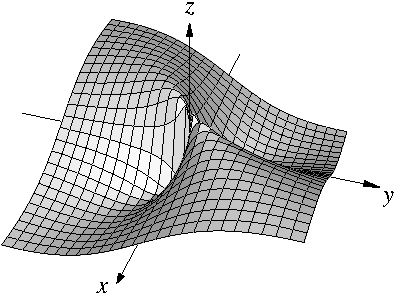
\includegraphics{figures/xyxsqysq}
\caption{Graph of $\frac{xy}{x^2+y^2}$.\label{fig:xyxsqysqvol2}}
\end{myfig}

\subsection{Inverse function theorem}
\label{subsec:svinvfuncthm}

To prove the inverse function theorem we use the contraction mapping
principle (\thmref{thm:contr}).
Intuitively if a function is continuously differentiable, then it
locally ``behaves like'' the derivative (which is a linear function).
The idea of the inverse function theorem is that if a function is
continuously differentiable and the derivative is invertible, the function is
(locally) invertible.

\begin{thm}[Inverse function theorem]\index{inverse function theorem}
\label{thm:inverse}
Let $U \subset \R^n$ be an open set and let
$f \colon U \to \R^n$ be a continuously differentiable function.
Suppose $p \in U$ and $Df|_p$ is invertible
(that is, $\det Df|_p \not=0$).
Then there exist open sets $V, W \subset \R^n$ such that
$p \in V \subset U$, $f(V) = W$, the restriction $f|_V$ is one-to-one,
and hence a $g \colon W \to V$ exists such that
$g(y) = (f|_V)^{-1}(y)$.
See \figureref{fig:inversefuncRn}.
Furthermore, $g$ is continuously differentiable
and 
\begin{equation*}
Dg|_y = {\bigl(Df|_x\bigr)}^{-1}, \qquad \text{for all } x \in V, y = f(x).
\end{equation*}
\end{thm}

\begin{myfig}
\subimport*{figures/}{inversefuncRn.pdf_t}
\caption{Setup of the inverse function theorem in $\R^n$.\label{fig:inversefuncRn}}
\end{myfig}

\begin{proof}
Write $A = Df|_p$.  As $Df$ is continuous, there exists an open ball
$V$ around $p$ such that
\begin{equation*}
\snorm{A-Df|_x} < \frac{1}{2\snorm{A^{-1}}}
\qquad \text{for all } x \in V.
\end{equation*}
The inequality implies that $Df|_x$ is invertible for all $x \in V$.
%FIXME: should we say more? %by \propref{prop:finitedimpropinv}.

Given $y \in \R^n$ we define $\varphi_y \colon C \to \R^n$ by
\begin{equation*}
\varphi_y (x) = x + A^{-1}\bigl(y-f(x)\bigr) .
\end{equation*}
As $A^{-1}$ is one-to-one,
$\varphi_y(x) = x$ ($x$ is a fixed point) if only if
$y-f(x) = 0$, or in other words $f(x)=y$.  Using the chain rule we obtain
\begin{equation*}
D\varphi_y|_x = I - A^{-1} Df|_x = A^{-1} \bigl( A-Df|_x \bigr) .
\end{equation*}
So for $x \in V$ we have
\begin{equation*}
\snorm{D\varphi_y|_x} \leq \snorm{A^{-1}} \, \snorm{A-Df|_x} < \nicefrac{1}{2} .
\end{equation*}
As $V$ is a ball, it is convex.  Hence
\begin{equation*}
\snorm{\varphi_y(x_1)-\varphi_y(x_2)} \leq \frac{1}{2} \snorm{x_1-x_2} 
\qquad
\text{for all } x_1,x_2 \in V.
\end{equation*}
In other words $\varphi_y$ is a contraction defined on $V$, though we so far
do not know what is the range of $\varphi_y$.  We cannot yet
apply the fixed
point theorem, but we can say that $\varphi_y$ 
has at most one fixed point in $V$:
If $\varphi_y(x_1) = x_1$ and
$\varphi_y(x_2) = x_2$, then
$\snorm{x_1-x_2} = \snorm{\varphi_y(x_1)-\varphi_y(x_2)} \leq
\frac{1}{2} \snorm{x_1-x_2}$, so $x_1 = x_2$.
That is, there exists at most one $x \in V$
such that $f(x) = y$, and so $f|_V$ is one-to-one.

Let $W = f(V)$.  We need to show that $W$ is open.  Take a $y_0 \in W$.
There is a unique $x_0 \in V$ such that $f(x_0) = y_0$.
Let $r > 0$ be small enough such that the closed ball $C(x_0,r) \subset V$
(such $r > 0$ exists as $V$ is open).

Suppose $y$ is such that
\begin{equation*}
\snorm{y-y_0} <
\frac{r}{2\snorm{A^{-1}}} .
\end{equation*}
If we show that $y \in W$, then we have shown that $W$ is open.
If $x \in
C(x_0,r)$, then
\begin{equation*}
\begin{split}
\snorm{\varphi_y(x)-x_0}
& \leq
\snorm{\varphi_y(x)-\varphi_y(x_0)} +
\snorm{\varphi_y(x_0)-x_0} \\
& \leq
\frac{1}{2}\snorm{x-x_0} +
\snorm{A^{-1}(y-y_0)} \\
& \leq
\frac{1}{2}r +
\snorm{A^{-1}} \, \snorm{y-y_0} \\
& <
\frac{1}{2}r +
\snorm{A^{-1}}
\frac{r}{2\snorm{A^{-1}}} = r .
\end{split}
\end{equation*}
So $\varphi_y$ takes $C(x_0,r)$ into $B(x_0,r) \subset C(x_0,r)$.  It is a
contraction on $C(x_0,r)$ and $C(x_0,r)$ is complete (closed subset of $\R^n$
is complete).
Apply the contraction mapping principle to obtain a fixed point $x$,
i.e.\ $\varphi_y(x) = x$.  That is, $f(x) = y$, and $y \in
f\bigl(C(x_0,r)\bigr) \subset f(V) = W$.  Therefore $W$ is open.

Next we need to show that $g$ is continuously differentiable and compute
its derivative.  First let us show that it is differentiable.
Let $y \in W$ and $k \in \R^n$, $k\not= 0$, such that $y+k \in W$.
Because $f|_V$ is a one-to-one and onto mapping of $V$ onto $W$,
there are unique
$x \in V$ and $h \in \R^n$, $h \not= 0$ and $x+h \in V$, such that
$f(x) = y$ and $f(x+h) = y+k$.
In other words, $g(y) = x$ and $g(y+k) = x+h$.  See
\figureref{fig:inversefuncRn2}.
\begin{myfig}
\subimport*{figures/}{inversefuncRn2.pdf_t}
\caption{Proving that $g$ is differentiable.\label{fig:inversefuncRn2}}
\end{myfig}

We can still
squeeze some information from the fact that $\varphi_y$ is a contraction.
\begin{equation*}
\varphi_y(x+h)-\varphi_y(x) = h + A^{-1} \bigl( f(x)-f(x+h) \bigr) = h - A^{-1} k .
\end{equation*}
So
\begin{equation*}
\snorm{h-A^{-1}k} = \snorm{\varphi_y(x+h)-\varphi_y(x)} \leq
\frac{1}{2}\snorm{x+h-x} = \frac{\snorm{h}}{2}.
\end{equation*}
By the inverse triangle inequality $\snorm{h} - \snorm{A^{-1}k} \leq
\frac{1}{2}\snorm{h}$, so
\begin{equation*}
\snorm{h} \leq 2 \snorm{A^{-1}k} \leq 2 \snorm{A^{-1}} \, \snorm{k}.
\end{equation*}
In particular, as $k$ goes to $0$, so does $h$.

As $x \in V$, then $Df|_x$ is invertible.
Let $B = \bigl(Df|_x\bigr)^{-1}$, which is what we think the derivative of
$g$ at $y$ is.  Then
\begin{equation*}
\begin{split}
\frac{\snorm{g(y+k)-g(y)-Bk}}{\snorm{k}}
& =
\frac{\snorm{h-Bk}}{\snorm{k}}
\\
& =
\frac{\snorm{h-B\bigl(f(x+h)-f(x)\bigr)}}{\snorm{k}}
\\
& =
\frac{\snorm{B\bigl(f(x+h)-f(x)-Df|_x h\bigr)}}{\snorm{k}}
\\
& \leq
\snorm{B}
\frac{\snorm{h}}{\snorm{k}}\,
\frac{\snorm{f(x+h)-f(x)-Df|_x h}}{\snorm{h}}
\\
& \leq
2\snorm{B} \, \snorm{A^{-1}}
\frac{\snorm{f(x+h)-f(x)-Df|_x h}}{\snorm{h}} .
\end{split}
\end{equation*}
As $k$ goes to $0$, so does $h$.  So the right hand side goes to $0$ as $f$ is
differentiable, and hence
the left hand side also goes to $0$.  And
$B$ is precisely what we wanted $Dg|_y$ to be.

We have $g$ is differentiable, let us show it is $C^1(W)$.
The function $g \colon W \to V$ is continuous (it is differentiable),
$Df$ is a continuous function from $V$
to the linear operators on $\R^n$,
and $X \mapsto X^{-1}$ is a continuous function on
the set of invertible operators.
As
$Dg|_y = {\bigl( Df|_{g(y)}\bigr)}^{-1}$ is the composition
of these three
continuous functions, it is continuous.
\end{proof}

\begin{example}
Also note that just because $Df|_x$ is invertible everywhere does not
mean that $f$ is
one-to-one globally.  It is ``locally'' one-to-one but perhaps not
``globally.''  For an
example, take the map $f \colon \R^2 \setminus \{ 0 \} \to \R^2$ defined
by $f(x,y) = (x^2-y^2,2xy)$.
It is left to student to show that $f$ is
differentiable and the derivative is invertible.

On the other hand, the mapping is 2-to-1 globally (except at the origin).
For every
$(a,b)$ that is not the origin, there are exactly two
solutions to $x^2-y^2=a$ and $2xy=b$.  We leave it to the reader
to show that there is at least one solution, and then notice
that replacing $x$ and $y$ with $-x$ and $-y$ obtains another solution.
\end{example}

The invertibility of the derivative is not a necessary
condition, just sufficient, for having a continuous inverse and being an open
mapping.  For example, the function $f(x) = x^3$ is an open mapping from $\R$
to $\R$ and is globally one-to-one with a continuous inverse, although the
inverse is not differentiable at $x=0$.

\medskip

As a side note, there is a related famous, and as yet unsolved problem,
called the \emph{\myindex{Jacobian conjecture}}.  If $F \colon \R^n \to
\R^n$ is polynomial (each component is a polynomial) and $\det DF$ is a nonzero
constant, does $F$ have a polynomial inverse?
The inverse function theorem gives a local $C^1$ inverse, but can one always
find a global polynomial inverse is the question.

\begin{exbox}
\begin{exercise}
\begin{exparts}
\item
Given a linear operator $A$ such that
$\snorm{I-A} < 1$, then $A$ is invertible ($I$ is the identity).
\item
For two linear operators $A$ and $B$ on $\R^n$ where $A$ is invertible,
prove that $\snorm{A-B} < \frac{1}{\snorm{A^{-1}}}$ implies that $B$ is
invertible.
\end{exparts}
\end{exercise}

\begin{exercise}
Define $f \colon \R^2 \to \R^2$ by $f(x,y) =
\bigl(x,y+h(x)\bigr)$ for some continuously differentiable function $h$ of one
variable.
\begin{exparts}
\item
Show that $f$ is one-to-one and onto.
\item
Compute $Df$.
\item
Show that $Df$ is invertible at all points, and compute
its inverse.
\end{exparts}
\end{exercise}

\begin{exercise}
Define $f \colon \R^2 \to \R^2$
\begin{equation*}
f(x,y) =
\begin{cases}
(x^2 \sin \bigl(\nicefrac{1}{x}\bigr) + \frac{x}{2} , y ) & \text{if } x \not= 0, \\
(0,y)                                                     & \text{if } x=0.
\end{cases}
\end{equation*}
\begin{exparts}
\item
Show that $f$ is differentiable everywhere.
\item
Show that $Df|_{(0,0)}$ is invertible.
\item
Show that $f$ is not one-to-one in any neighborhood of the origin (it is
not locally invertible, that is, the inverse function theorem does not work).
\item
Show that $f$ is not continuously differentiable.
\end{exparts}
\end{exercise}

\begin{exercise}[Polar coordinates] \label{mv:exercise:polarcoordinates}
\index{polar coordinates}
Define a mapping $F(r,\theta) = \bigl(r \cos(\theta), r \sin(\theta) \bigr)$.
\begin{exparts}
\item
Show that $F$ is continuously differentiable (for all $(r,\theta) \in
\R^2$).
\item
Compute $DF|_{(0,\theta)}$ for any $\theta$.
\item
Show that if $r \not= 0$, then $DF|_{(r,\theta)}$ is invertible, therefore an
inverse of $F$ exists locally as long as $r \not= 0$.
\item
Show that $F \colon \R^2 \to \R^2$ is onto, and for each point $(x,y) \in
\R^2$, the set $F^{-1}(x,y)$ is infinite.
\item
Show that $F|_{(0,\infty) \times [0,2\pi)}$ is one to one and onto
$\R^2 \setminus \bigl\{ (0,0) \bigr\}$.
\end{exparts}
\end{exercise}
\end{exbox}

%%%%%%%%%%%%%%%%%%%%%%%%%%%%%%%%%%%%%%%%%%%%%%%%%%%%%%%%%%%%%%%%%%%%%%%%%%%%%%
%%%%%%%%%%%%%%%%%%%%%%%%%%%%%%%%%%%%%%%%%%%%%%%%%%%%%%%%%%%%%%%%%%%%%%%%%%%%%%
%%%%%%%%%%%%%%%%%%%%%%%%%%%%%%%%%%%%%%%%%%%%%%%%%%%%%%%%%%%%%%%%%%%%%%%%%%%%%%

\chapter{Basic notation and terminology} \label{ap:basicnotation}

%%%%%%%%%%%%%%%%%%%%%%%%%%%%%%%%%%%%%%%%%%%%%%%%%%%%%%%%%%%%%%%%%%%%%%%%%%%%%%

% Is this overly too nitpicky to include?

Let us just quickly review some of the basic notation that we use in this
book, that is perhaps not described elsewhere.
We use $\C$, $\R$ for complex and real numbers, and $i$ for imaginary unit
(a square root of $-1$).  We use
$\N = \{ 1,2,3, \ldots \}$ for 
the natural numbers,
$\Z$ for all integers, and
$\Q$ for rational real numbers,

\glsadd{not:setminus}%
We denote the set subtraction by 
$A \setminus B$,
meaning all elements of
$A$ that are not in $B$.
We the complement of a set is $X^c$, in which case
the ambient set should be clear.
\glsadd{not:closure}%
The topological closure of a set $S$ is denoted by $\overline{S}$, its
boundary is denoted by
\glsadd{not:boundary}%
$\partial S$.  By $\partial S$ we may also mean the path that gives the
topological boundary traversed counterclockwise.
We write the interior of $S$ as
\glsadd{not:interior}%
$S^\circ$.

\glsadd{not:function}%
The notation $f \colon X \to Y$ is a function with domain $X$ and
codomain $Y$.  By $f(S)$ we mean the direct image of $S$ by $f$.
The notation $f^{-1}$ means the inverse image of sets and
single points, and when the mapping is bijective (one-to-one and onto),
we use it for the inverse mapping.  So for example $f^{-1}(T)$ for
a set $T \subset Y$ denotes all the points of $X$ that $f$ maps to $T$.
If $q$ is a point, then $f^{-1}(q)$ denotes the set of all the points that map to $q$.
If the mapping is bijective, then $f^{-1}(q)$ just denotes the unique point
mapping to $q$.
To define a function without necessarily giving it a name, we use
\glsadd{not:mapsto}%
\begin{equation*}
x \mapsto F(x) ,
\end{equation*}
where $F(x)$ would generally be some formula giving the output.
The notation
\glsadd{not:restriction}%
\begin{equation*}
f|_S
\end{equation*}
means the restriction of $f$ to $S$:
a function
$f|_S \colon S \to Y$ such that $f|_S(x) = f(x)$ for all $x \in S$.
To say that two functions are identically equal, we write
\glsadd{not:identeq}%
\begin{equation*}
f \equiv g .
\end{equation*}
This means that $f(x) = g(x)$ for all $x$ in the domain.
The notation
\glsadd{not:composition}%
\begin{equation*}
f \circ g
\end{equation*}
denotes the composition defined by $x \mapsto f\bigl(g(x)\bigr)$.

We write
\glsadd{not:definition}%
\begin{equation*}
X
\overset{\text{def}}{=}
Y
\end{equation*}
to define $X$ to be $Y$ rather than just show equality.

%%%%%%%%%%%%%%%%%%%%%%%%%%%%%%%%%%%%%%%%%%%%%%%%%%%%%%%%%%%%%%%%%%%%%%%%%%%%%%
%%%%%%%%%%%%%%%%%%%%%%%%%%%%%%%%%%%%%%%%%%%%%%%%%%%%%%%%%%%%%%%%%%%%%%%%%%%%%%
%%%%%%%%%%%%%%%%%%%%%%%%%%%%%%%%%%%%%%%%%%%%%%%%%%%%%%%%%%%%%%%%%%%%%%%%%%%%%%

%FIXME: else I don't get links, weird
%\def\MR#1{\relax\ifhmode\unskip\spacefactor3000 \space\fi%
  %\href{http://www.ams.org/mathscinet-getitem?mr=#1}{MR#1}}
\def\myDOI#1{\href{http://dx.doi.org/#1}{#1}}



%FIXME
%\cleardoublepage  
\clearpage
\phantomsection
\addcontentsline{toc}{chapter}{Further reading}
\markboth{FURTHER READING}{FURTHER READING}
\begin{bibchapter}[Further Reading] \label{ch:furtherreading}

%Here we list useful books for extra reading.

\begin{biblist}[\normalsize]

\bib{Boas}{book}{
   author={Boas, Ralph P.},
   title={Invitation to complex analysis},
   series={MAA Textbooks},
   edition={2},
   note={Revised by Harold P. Boas},
   publisher={Mathematical Association of America, Washington, DC},
   date={2010},
   pages={xiv+327},
   isbn={978-0-88385-764-9},
   review={\MR{2674618}},
}

\bib{Conway1}{book}{
   author={Conway, John B.},
   title={Functions of one complex variable},
   series={Graduate Texts in Mathematics},
   volume={11},
   edition={2},
   publisher={Springer-Verlag, New York-Berlin},
   date={1978},
   pages={xiii+317},
   isbn={0-387-90328-3},
   review={\MR{503901}},
}

\bib{Conway2}{book}{
   author={Conway, John B.},
   title={Functions of one complex variable. II},
   series={Graduate Texts in Mathematics},
   volume={159},
   publisher={Springer-Verlag, New York},
   date={1995},
   pages={xvi+394},
   isbn={0-387-94460-5},
   review={\MR{1344449}},
   doi={10.1007/978-1-4612-0817-4},
}

\bib{ra:book}{misc}{
   author={Lebl, Ji\v{r}\'i},
   title={Basic Analysis I: Introduction to Real Analysis, Volume I},
   note={\url{https://www.jirka.org/ra/}}
}

\bib{ra:book2}{misc}{
   author={Lebl, Ji\v{r}\'i},
   title={Basic Analysis II: Introduction to Real Analysis, Volume II},
   note={\url{https://www.jirka.org/ra/}}
}

\bib{scv:book}{misc}{
   author={Lebl, Ji\v{r}\'i},
   title={Tasty bits of Several Complex Variables},
   note={\url{https://www.jirka.org/scv/}}
}

\bib{Rudin:principles}{book}{
   author={Rudin, Walter},
   title={Principles of mathematical analysis},
   edition={3},
   note={International Series in Pure and Applied Mathematics},
   publisher={McGraw-Hill Book Co., New York-Auckland-D\"usseldorf},
   date={1976},
   pages={x+342},
   review={\MR{0385023}},
}

\bib{Rudin}{book}{
   author={Rudin, Walter},
   title={Real and complex analysis},
   edition={3},
   publisher={McGraw-Hill Book Co., New York},
   date={1987},
   pages={xiv+416},
   isbn={0-07-054234-1},
   review={\MR{924157}},
}

\bib{Ullrich}{book}{
   author={Ullrich, David C.},
   title={Complex made simple},
   series={Graduate Studies in Mathematics},
   volume={97},
   publisher={American Mathematical Society, Providence, RI},
   date={2008},
   pages={xii+489},
   isbn={978-0-8218-4479-3},
   review={\MR{2450873}},
   doi={10.1090/gsm/097},
}

\end{biblist}
\end{bibchapter}

%%%%%%%%%%%%%%%%%%%%%%%%%%%%%%%%%%%%%%%%%%%%%%%%%%%%%%%%%%%%%%%%%%%%%%%%%%%%%%
%%%%%%%%%%%%%%%%%%%%%%%%%%%%%%%%%%%%%%%%%%%%%%%%%%%%%%%%%%%%%%%%%%%%%%%%%%%%%%
%%%%%%%%%%%%%%%%%%%%%%%%%%%%%%%%%%%%%%%%%%%%%%%%%%%%%%%%%%%%%%%%%%%%%%%%%%%%%%

%\cleardoublepage  
\clearpage  
\phantomsection
\addcontentsline{toc}{chapter}{\indexname}  
\microtypesetup{protrusion=false}
\printindex
\microtypesetup{protrusion=true}

%%%%%%%%%%%%%%%%%%%%%%%%%%%%%%%%%%%%%%%%%%%%%%%%%%%%%%%%%%%%%%%%%%%%%%%%%%%%%%
%%%%%%%%%%%%%%%%%%%%%%%%%%%%%%%%%%%%%%%%%%%%%%%%%%%%%%%%%%%%%%%%%%%%%%%%%%%%%%
%%%%%%%%%%%%%%%%%%%%%%%%%%%%%%%%%%%%%%%%%%%%%%%%%%%%%%%%%%%%%%%%%%%%%%%%%%%%%%

%
% automake on glossaries doesn't work if the index is before the glossary.
% That's why the List of Notation is last, no other reason.  Problem is
% that printindex does a clearpage which screws up the delayed write18
% that glossaries sets up
%

\begingroup
\renewcommand{\pagelistname}{Page}
\setglossarystyle{long3colheader}
% correctly set up with cellspace
\renewenvironment{theglossary}%
  {\setlength\cellspacetoplimit{4pt}
   \setlength\cellspacebottomlimit{4pt}
   \setlength\LTleft{0pt}
   \setlength\LTright{0pt}
   \markboth{LIST OF NOTATION}{LIST OF NOTATION}
   \begin{longtable}{Sl @{\extracolsep{\fill}} Sl @{\extracolsep{\fill}} Sl}}%
  {\end{longtable}}%
\cleardoublepage
\microtypesetup{protrusion=false}
\printglossary[type=notation] 
\microtypesetup{protrusion=true}
\endgroup

\end{document}
